% ******************************* PhD Thesis Template **************************
% Please have a look at the README.md file for info on how to use the template

\documentclass[a4paper,12pt,times,print,authoryear,index]{Classes/PhDThesisPSnPDF}

\usepackage[T1]{fontenc}

% ******************************************************************************
% ******************************* Class Options ********************************
% *********************** See README for more details **************************
% ******************************************************************************

% `a4paper'(The University of Cambridge PhD thesis guidelines recommends a page
% size a4 - default option) or `a5paper': A5 Paper size is also allowed as per
% the Cambridge University Engineering Department guidelines for PhD thesis
%
% `11pt' or `12pt'(default): Font Size 10pt is NOT recommended by the University
% guidelines
%
% `oneside' or `twoside'(default): Printing double side (twoside) or single
% side.
%
% `print': Use `print' for print version with appropriate margins and page
% layout. Leaving the options field blank will activate Online version.
%
% `index': For index at the end of the thesis
%
% `draftclassic': For draft mode without loading any images (same as draft in book)
%
% `draft': Special draft mode with line numbers, images, and water mark with
% timestamp and custom text. Position of the text can also be modified.
%
% `abstract': To generate only the title page and abstract page with
% dissertation title and name, to submit to the Student Registry
%
% `chapter`: This option enables only the specified chapter and it's references
%  Useful for review and corrections.
%
% ************************* Custom Page Margins ********************************
%
% `custommargin`: Use `custommargin' in options to activate custom page margins,
% which can be defined in the preamble.tex. Custom margin will override
% print/online margin setup.
%
% *********************** Choosing the Fonts in Class Options ******************
%
% `times' : Times font with math support. (The Cambridge University guidelines
% recommend using times)
%
% `fourier': Utopia Font with Fourier Math font (Font has to be installed)
%            It's a free font.
%
% `customfont': Use `customfont' option in the document class and load the
% package in the preamble.tex
%
% default or leave empty: `Latin Modern' font will be loaded.
%
% ********************** Choosing the Bibliography style ***********************
%
% `authoryear': For author-year citation eg., Krishna (2013)
%
% `numbered': (Default Option) For numbered and sorted citation e.g., [1,5,2]
%
% `custombib': Define your own bibliography style in the `preamble.tex' file.
%              `\RequirePackage[square, sort, numbers, authoryear]{natbib}'.
%              This can be also used to load biblatex instead of natbib
%              (See Preamble)
%
% **************************** Choosing the Page Style *************************
%
% `default (leave empty)': For Page Numbers in Header (Left Even, Right Odd) and
% Chapter Name in Header (Right Even) and Section Name (Left Odd). Blank Footer.
%
% `PageStyleI': Chapter Name next & Page Number on Even Side (Left Even).
% Section Name & Page Number in Header on Odd Side (Right Odd). Footer is empty.
%
% `PageStyleII': Chapter Name on Even Side (Left Even) in Header. Section Number
% and Section Name in Header on Odd Side (Right Odd). Page numbering in footer

% Uncomment to change page style
%\pagestyle{PageStyleII}

% ********************************** Preamble **********************************
% Preamble: Contains packages and user-defined commands and settings
% ******************************************************************************
% ****************************** Custom Margin *********************************

% Add `custommargin' in the document class options to use this section
% Set {innerside margin / outerside margin / topmargin / bottom margin}  and
% other page dimensions
\ifsetCustomMargin
  \RequirePackage[left=37mm,right=30mm,top=35mm,bottom=30mm]{geometry}
  \setFancyHdr % To apply fancy header after geometry package is loaded
\fi

% Add spaces between paragraphs
%\setlength{\parskip}{0.5em}
% Ragged bottom avoids extra whitespaces between paragraphs
\raggedbottom
% To remove the excess top spacing for enumeration, list and description
%\usepackage{enumitem}
%\setlist[enumerate,itemize,description]{topsep=0em}

% *****************************************************************************
% ******************* Fonts (like different typewriter fonts etc.)*************

% Add `customfont' in the document class option to use this section

% \ifsetCustomFont
  % Set your custom font here and use `customfont' in options. Leave empty to
  % load computer modern font (default LaTeX font).
  %\RequirePackage{helvet}

  % For use with XeLaTeX
  %  \setmainfont[
  %    Path              = ./libertine/opentype/,
  %    Extension         = .otf,
  %    UprightFont = LinLibertine_R,
  %    BoldFont = LinLibertine_RZ, % Linux Libertine O Regular Semibold
  %    ItalicFont = LinLibertine_RI,
  %    BoldItalicFont = LinLibertine_RZI, % Linux Libertine O Regular Semibold Italic
  %  ]
  %  {libertine}
  %  % load font from system font
  %  \newfontfamily\libertinesystemfont{Linux Libertine O}
% \fi
% 
% *****************************************************************************
% **************************** Custom Packages ********************************

%\usepackage{algpseudocode}
% \RequirePackage[labelsep=space,tableposition=top]{caption}
% \renewcommand{\figurename}{Fig.} %to support older versions of captions.sty

% ******************************* Line Spacing *********************************

% Choose linespacing as appropriate. Default is one-half line spacing as per the
% University guidelines

% \doublespacing
% \onehalfspacing
% \singlespacing


% ************************ Formatting / Footnote *******************************
% Don't break enumeration (etc.) across pages in an ugly manner (default 10000)
%\clubpenalty=500
%\widowpenalty=500
%\usepackage[perpage]{footmisc} %Range of footnote options


% *****************************************************************************
% *************************** Bibliography  and References ********************

%\usepackage{cleveref} %Referencing without need to explicitly state fig /table

% Add `custombib' in the document class option to use this section
% \ifuseCustomBib
%    \RequirePackage[square, sort, numbers, authoryear]{natbib} % CustomBib

% If you would like to use biblatex for your reference management, as opposed to the default `natbibpackage` pass the option `custombib` in the document class. Comment out the previous line to make sure you don't load the natbib package. Uncomment the following lines and specify the location of references.bib file

%\RequirePackage[backend=biber, style=numeric-comp, citestyle=numeric, sorting=nty, natbib=true]{biblatex}
%\addbibresource{References/references} %Location of references.bib only for biblatex, Do not omit the .bib extension from the filename.

% \fi

% ******************************************************************************
% ************************* User Defined Commands ******************************
% ******************************************************************************

% *********** To change the name of Table of Contents / LOF and LOT ************

%\renewcommand{\contentsname}{My Table of Contents}
%\renewcommand{\listfigurename}{My List of Figures}
%\renewcommand{\listtablename}{My List of Tables}


% ********************** TOC depth and numbering depth *************************

\setcounter{secnumdepth}{2}
\setcounter{tocdepth}{2}


% ******************************* Nomenclature *********************************

% To change the name of the Nomenclature section, uncomment the following line

%\renewcommand{\nomname}{Symbols}


% ********************************* Appendix ***********************************

% The default value of both \appendixtocname and \appendixpagename is `Appendices'. These names can all be changed via:

%\renewcommand{\appendixtocname}{List of appendices}
%\renewcommand{\appendixname}{Appndx}

% *********************** Configure Draft Mode **********************************

% Uncomment to disable figures in `draft'
%\setkeys{Gin}{draft=true}  % set draft to false to enable figures in `draft'

% These options are active only during the draft mode
% Default text is "Draft"
%\SetDraftText{DRAFT}

% Default Watermark location is top. Location (top/bottom)
%\SetDraftWMPosition{bottom}

% Draft Version - default is v1.0
%\SetDraftVersion{v1.1}

% Draft Text grayscale value (should be between 0-black and 1-white)
% Default value is 0.75
%\SetDraftGrayScale{0.8}


% *****************************************************************************
% ******************* Better enumeration my MB*************
% \usepackage{enumitem}
% \usepackage{sty/aaai24}
\usepackage{tabularx}
\usepackage{rotating}
\usepackage{pdfpages}
\usepackage{graphicx}
\usepackage{array}
\usepackage{cleveref}
\usepackage{booktabs}
\usepackage[utf8]{inputenc}
\usepackage{hyperref}
\usepackage{caption}
\usepackage{floatrow}
\usepackage{multirow}
\usepackage{xcolor}
\usepackage{colortbl}
\usepackage{algorithm}
\usepackage[noend]{algpseudocode}
\usepackage{amsmath}
\usepackage{amsthm}
\usepackage{amssymb}
\usepackage{pifont}
\usepackage{quoting}
\usepackage{epigraph}
\usepackage[flushleft]{threeparttable}
% \usepackage{subfig}
\usepackage{subcaption}
\usepackage[shortlabels]{enumitem}
\usepackage{relsize}
\usepackage{siunitx}

% \usepackage{microtype} % microtypography
\usepackage{xspace}
% \usepackage{paralist}



\newtheorem{example}{Example}
\newtheorem{definition}{Definition}
\newtheorem{problem}{Problem}
\newtheorem{theorem}{Theorem}
\newtheorem{lemma}{Lemma}

% \newenvironment{proof}{{\bf Proof:}}{}

\newcommand{\HPO}{HPO\xspace}
\newcommand{\NLP}{NLP\xspace}
\newcommand{\ML}{ML\xspace}
\newcommand{\AutoML}{AutoML\xspace}
\newcommand{\LM}{LM\xspace}
\newcommand{\LMs}{LMs\xspace}
\newcommand{\LLM}{LLM\xspace}
\newcommand{\LLMs}{LLMs\xspace}
\newcommand{\NAS}{NAS\xspace}
\newcommand\todo[1]{{\color{red}[ToDo: #1]}}


\newcommand{\cupdot}{\mathbin{\mathaccent\cdot\cup}}
\newcommand{\cmark}{\ding{51}}
\newcommand{\xmark}{\ding{55}}
\newcommand{\eop}{\hfill $\Box$}
\newcommand{\mf}[1]{\textcolor{red}{\textbf{#1} ??}}
\newcommand{\argmax}{\mathop{\mathrm{argmax}}}
\newcommand{\argmin}{\mathop{\mathrm{argmin}}}
\newcommand{\veryshortarrow}[1][3pt]{\mathrel{%
		\hbox{\rule[\dimexpr\fontdimen22\textfont2-.2pt\relax]{#1}{.4pt}}%
		\mkern-4mu\hbox{\usefont{U}{lasy}{m}{n}\symbol{41}}}}
\newcommand{\argtup}{{Arg{\sf 2}P}}

\renewcommand{\sf}[1]{\textsf{\textup{#1}}}
\renewcommand{\tt}[1]{\texttt{\textup{#1}}}
\renewcommand{\pm}{\mathbin{\smash{\raisebox{0.35ex}{$\underset{\raisebox{0.5ex}{$\smash -$}}{\smash+}$}}}}
\renewcommand{\vec}[1]{\boldsymbol{#1}}

\DeclareMathAlphabet{\altmathcal}{OMS}{cmsy}{m}{n}


\algnewcommand\algorithmicforeach{\textbf{for each}}
\algdef{S}[FOR]{ForEach}[1]{\algorithmicforeach\ #1\ \algorithmicdo}

\newfloatcommand{capbtabbox}{table}[][\FBwidth]

\newif\ifproofread
\proofreadtrue % commentare questo per disattivare \mf \mg \eg \sr

\usepackage{listings}

\crefname{lstlisting}{listing}{listings}
\Crefname{lstlisting}{Listing}{Listings}

\lstset{%
    basicstyle=\small\ttfamily,
    frame=single,
    morecomment=[f][\color{Green}][0]{\#},
    tabsize = 4, %% set tab space width
    commentstyle = \color{green}, %% set comment color
    keywordstyle = \color{blue}, %% set keyword color
    stringstyle = \color{red}, %% set string color
    rulecolor = \color{black}, %% set frame color to avoid being affected by text color
    basicstyle = \small \ttfamily , %% set listing font and size
    breaklines = true, %% enable line breaking
    numberstyle = \tiny,
}

% \usepackage{booktabs}
% \usepackage{comment}
% \usepackage{amsmath}
% \usepackage{amsthm}
% \usepackage{amssymb}
% \usepackage{listings}
% \usepackage{hyperref}
% \usepackage{cleveref}
% \usepackage{caption}
% \usepackage{threeparttable,booktabs}
% \usepackage{algpseudocode}
% \usepackage{algorithm}
% \usepackage{balance}
% \usepackage[normalem]{ulem}
% \usepackage[dvipsnames]{xcolor}


% %%%%%%%%%%%%%%%%%%%%%%%%%%%%%%%%%%%%%%%%%%%%%%%%%%%%%%%%
% Uncomment to check unused bibitems from here
% \usepackage{refcheck}
% \makeatletter
% \newcommand{\refcheckize}[1]{%
%   \expandafter\let\csname @@\string#1\endcsname#1%
%   \expandafter\DeclareRobustCommand\csname relax\string#1\endcsname[1]{%
%     \csname @@\string#1\endcsname{##1}\wrtusdrf{##1}}%
%   \expandafter\let\expandafter#1\csname relax\string#1\endcsname
% }
% \makeatother
% \refcheckize{\cref}
% \refcheckize{\Cref}
% ... to here
% %%%%%%%%%%%%%%%%%%%%%%%%%%%%%%%%%%%%%%%%%%%%%%%%%%%%%%%%

% \usepackage{booktabs} % For formal tables
% \usepackage{fancyhdr,amsmath}             % AMS Math
% \usepackage[utf8]{inputenc}
% \usepackage{xr}
% \usepackage{fullpage}
% \usepackage{times}
% \usepackage[ruled,vlined,linesnumbered]{algorithm2e}
% \usepackage{mathrsfs}
% \usepackage{listings,xcolor}
% \usepackage{color}
% \usepackage{blindtext}
% \usepackage{makeidx}  % allows for indexgeneration
\usepackage{natbib}
\let\cite\citep
\let\shortcite\citeyearpar
\setcitestyle{aysep={}}
\setlength\bibhang{0pt}
\bibliographystyle{Classes/aaai24}
% \usepackage{rotating}
% \usepackage[noend]{algpseudocode}
% \usepackage{paralist}
% \usepackage{tabularx}
% \usepackage{url}
% \usepackage{soul}
% \usepackage[disable]{todonotes}
% \usepackage{todonotes}
% \usepackage{enumitem}
% \usepackage{tikz,fullpage}
% \usepackage{hyperref}
% \usepackage{amssymb}
% \usepackage{tkz-berge}
% \usetikzlibrary{shapes.geometric}
% \usepackage{caption}
% \usepackage{subcaption}
% \usepackage{stmaryrd}
% \usepackage{courier}
% \usepackage{algorithm}
% \usepackage{eqparbox}
% \usepackage{float}
% \usepackage{subcaption}
% \usepackage{algorithmic}


% ************************ Thesis Information & Meta-data **********************
% Thesis title and author information, reference file for biblatex
% % \newcolumntype{P}[1]{>{\centering\arraybackslash}p{#1}}
% % \begin{document}
% \begin{titlepage}
% 	\centering
% 	{\Large Alma Mater Studiorum - Universit\`a di Bologna \par}
% 	\vspace{1.5cm}
% 	{\normalsize Dottorato di ricerca in Computer Science and Engineering \par}
% 	\vspace{0.2cm}
% 	{Ciclo XXXIII \par}
% 	\vspace{0.4cm}
% 	{\scriptsize Settore concorsuale di afferenza: 09/H1 - SISTEMI DI ELABORAZIONE DELLE INFORMAZIONI\par}
% 	\vspace{0.1cm}
% 	{\scriptsize Settore scientifico disciplinare: ING-INF/05 - SISTEMI DI ELABORAZIONE DELLE INFORMAZIONI\par}
% 	\vspace{2cm}
% 	{\Large\bfseries Augmenting the Knowledge Pyramid\\with
% Unconventional Data and Advanced Analytics\par}
% 	\vspace{3cm}
% 	{\Large Matteo Francia\par}
% 	\vspace{3cm}
	
	
% 	\begin{table}[h]
% 		\centering
% 		\begin{center} 
% 		\begin{tabular}{  
% 			P{\dimexpr 0.5\linewidth-2\tabcolsep} P{\dimexpr 0.5\linewidth-2\tabcolsep} }
% 			{\large Coordinatore Dottorato} & {\large Relatore} \\
% 			\vspace{0.1cm}{\large Prof. Davide Sangiorgi} & \vspace{0.1cm}{\large Prof. Matteo Golfarelli}\\
% 		\end{tabular} 
% 		\end{center}
% 	\end{table}
% 	\vfill
% %	{\large \today\par}
% 	{\large Esame finale 2021}
% \end{titlepage}

% \author{Matteo Francia}


\newcommand{\clearemptydoublepage}{\newpage{\pagestyle{empty}%
\cleardoublepage}}

\begin{titlepage}
%
% HEADER
%
\begin{center}
{{\Large{\textsc{Alma Mater Studiorum -- Università di Bologna}}\\\normalsize{\textsc{Dipartimento di Informatica -- Scienza e Ingegneria (DISI)}}}}
\rule[0.1cm]{15.8cm}{0.1mm}
\rule[0.5cm]{15.8cm}{0.6mm}
{\large{\textsc {Dottorato di Ricerca in\\Computer Science and Engineering}}\\
\vspace{3mm}
\normalsize{\textsc {Ciclo XXXVI}}}
\end{center}
%
\vspace{7mm}
%
% COURSE INFO
%
\begin{footnotesize}
\centering
Settore Concorsuale di Afferenza: 09/H1 - SISTEMI DI ELABORAZIONE DELLE INFORMAZIONI\\
Settore Scientifico Disciplinare: ING-INF/05 - SISTEMI DI ELABORAZIONE DELLE INFORMAZIONI
\end{footnotesize}
%
\vfill
%
% TITLE
%
\begin{center}
{\LARGE\textbf{On the democratization of AI:}\\\vskip 1pt
\Large\textbf{Bridging the Gap with AutoML}}
\end{center}
%
\vfill
%
% CANDIDATE
%
\begin{center}
{\large{\emph{Candidato}}\\
{\bf \textsc{Joseph Giovanelli}}}
\end{center}
%
\vskip 16pt
%
% COORDINATOR, SUPERVISOR, TUTOR
%
\begin{minipage}[t]{0.47\textwidth}
{\large{\emph{Coordinatore Dottorato}}\\
{\bf \textsc{Prof. Ilaria Bartolini}}}
\end{minipage}
\hfill
\begin{minipage}[t]{0.47\textwidth}\raggedleft
{\large{\emph{Supervisore}}\\
{\bf \textsc{Prof. Matteo Golfarelli}}}
% \vskip 8pt
% {\large{\emph{Tutor}}\\
% {\bf \textsc{Prof. Stefano Rizzi}}}
\end{minipage}
%
\vfill
%
% DATE
%
\begin{center}
{\large{\sc Esame Finale Anno 2024}}
\end{center}
%
\clearemptydoublepage

\end{titlepage}

% ***************************** Abstract Separate ******************************
% To printout only the titlepage and the abstract with the PhD title and the
% author name for submission to the Student Registry, use the `abstract' option in
% the document class.

\ifdefineAbstract
 \pagestyle{empty}
 \includeonly{Declaration/declaration, Abstract/abstract}
\fi

% ***************************** Chapter Mode ***********************************
% The chapter mode allows user to only print particular chapters with references
% Title, Contents, Frontmatter are disabled by default
% Useful option to review a particular chapter or to send it to supervisor.
% To use choose `chapter' option in the document class

\ifdefineChapter
 \includeonly{Chapter3/chapter3}
\fi

% ******************************** Front Matter ********************************
\begin{document}

\frontmatter
% \newcolumntype{P}[1]{>{\centering\arraybackslash}p{#1}}
% % \begin{document}
% \begin{titlepage}
% 	\centering
% 	{\Large Alma Mater Studiorum - Universit\`a di Bologna \par}
% 	\vspace{1.5cm}
% 	{\normalsize Dottorato di ricerca in Computer Science and Engineering \par}
% 	\vspace{0.2cm}
% 	{Ciclo XXXIII \par}
% 	\vspace{0.4cm}
% 	{\scriptsize Settore concorsuale di afferenza: 09/H1 - SISTEMI DI ELABORAZIONE DELLE INFORMAZIONI\par}
% 	\vspace{0.1cm}
% 	{\scriptsize Settore scientifico disciplinare: ING-INF/05 - SISTEMI DI ELABORAZIONE DELLE INFORMAZIONI\par}
% 	\vspace{2cm}
% 	{\Large\bfseries Augmenting the Knowledge Pyramid\\with
% Unconventional Data and Advanced Analytics\par}
% 	\vspace{3cm}
% 	{\Large Matteo Francia\par}
% 	\vspace{3cm}
	
	
% 	\begin{table}[h]
% 		\centering
% 		\begin{center} 
% 		\begin{tabular}{  
% 			P{\dimexpr 0.5\linewidth-2\tabcolsep} P{\dimexpr 0.5\linewidth-2\tabcolsep} }
% 			{\large Coordinatore Dottorato} & {\large Relatore} \\
% 			\vspace{0.1cm}{\large Prof. Davide Sangiorgi} & \vspace{0.1cm}{\large Prof. Matteo Golfarelli}\\
% 		\end{tabular} 
% 		\end{center}
% 	\end{table}
% 	\vfill
% %	{\large \today\par}
% 	{\large Esame finale 2021}
% \end{titlepage}

% \author{Matteo Francia}


\newcommand{\clearemptydoublepage}{\newpage{\pagestyle{empty}%
\cleardoublepage}}

\begin{titlepage}
%
% HEADER
%
\begin{center}
{{\Large{\textsc{Alma Mater Studiorum -- Università di Bologna}}\\\normalsize{\textsc{Dipartimento di Informatica -- Scienza e Ingegneria (DISI)}}}}
\rule[0.1cm]{15.8cm}{0.1mm}
\rule[0.5cm]{15.8cm}{0.6mm}
{\large{\textsc {Dottorato di Ricerca in\\Computer Science and Engineering}}\\
\vspace{3mm}
\normalsize{\textsc {Ciclo XXXVI}}}
\end{center}
%
\vspace{7mm}
%
% COURSE INFO
%
\begin{footnotesize}
\centering
Settore Concorsuale di Afferenza: 09/H1 - SISTEMI DI ELABORAZIONE DELLE INFORMAZIONI\\
Settore Scientifico Disciplinare: ING-INF/05 - SISTEMI DI ELABORAZIONE DELLE INFORMAZIONI
\end{footnotesize}
%
\vfill
%
% TITLE
%
\begin{center}
{\LARGE\textbf{On the democratization of AI:}\\\vskip 1pt
\Large\textbf{Bridging the Gap with AutoML}}
\end{center}
%
\vfill
%
% CANDIDATE
%
\begin{center}
{\large{\emph{Candidato}}\\
{\bf \textsc{Joseph Giovanelli}}}
\end{center}
%
\vskip 16pt
%
% COORDINATOR, SUPERVISOR, TUTOR
%
\begin{minipage}[t]{0.47\textwidth}
{\large{\emph{Coordinatore Dottorato}}\\
{\bf \textsc{Prof. Ilaria Bartolini}}}
\end{minipage}
\hfill
\begin{minipage}[t]{0.47\textwidth}\raggedleft
{\large{\emph{Supervisore}}\\
{\bf \textsc{Prof. Matteo Golfarelli}}}
% \vskip 8pt
% {\large{\emph{Tutor}}\\
% {\bf \textsc{Prof. Stefano Rizzi}}}
\end{minipage}
%
\vfill
%
% DATE
%
\begin{center}
{\large{\sc Esame Finale Anno 2024}}
\end{center}
%
\clearemptydoublepage

\end{titlepage}
% 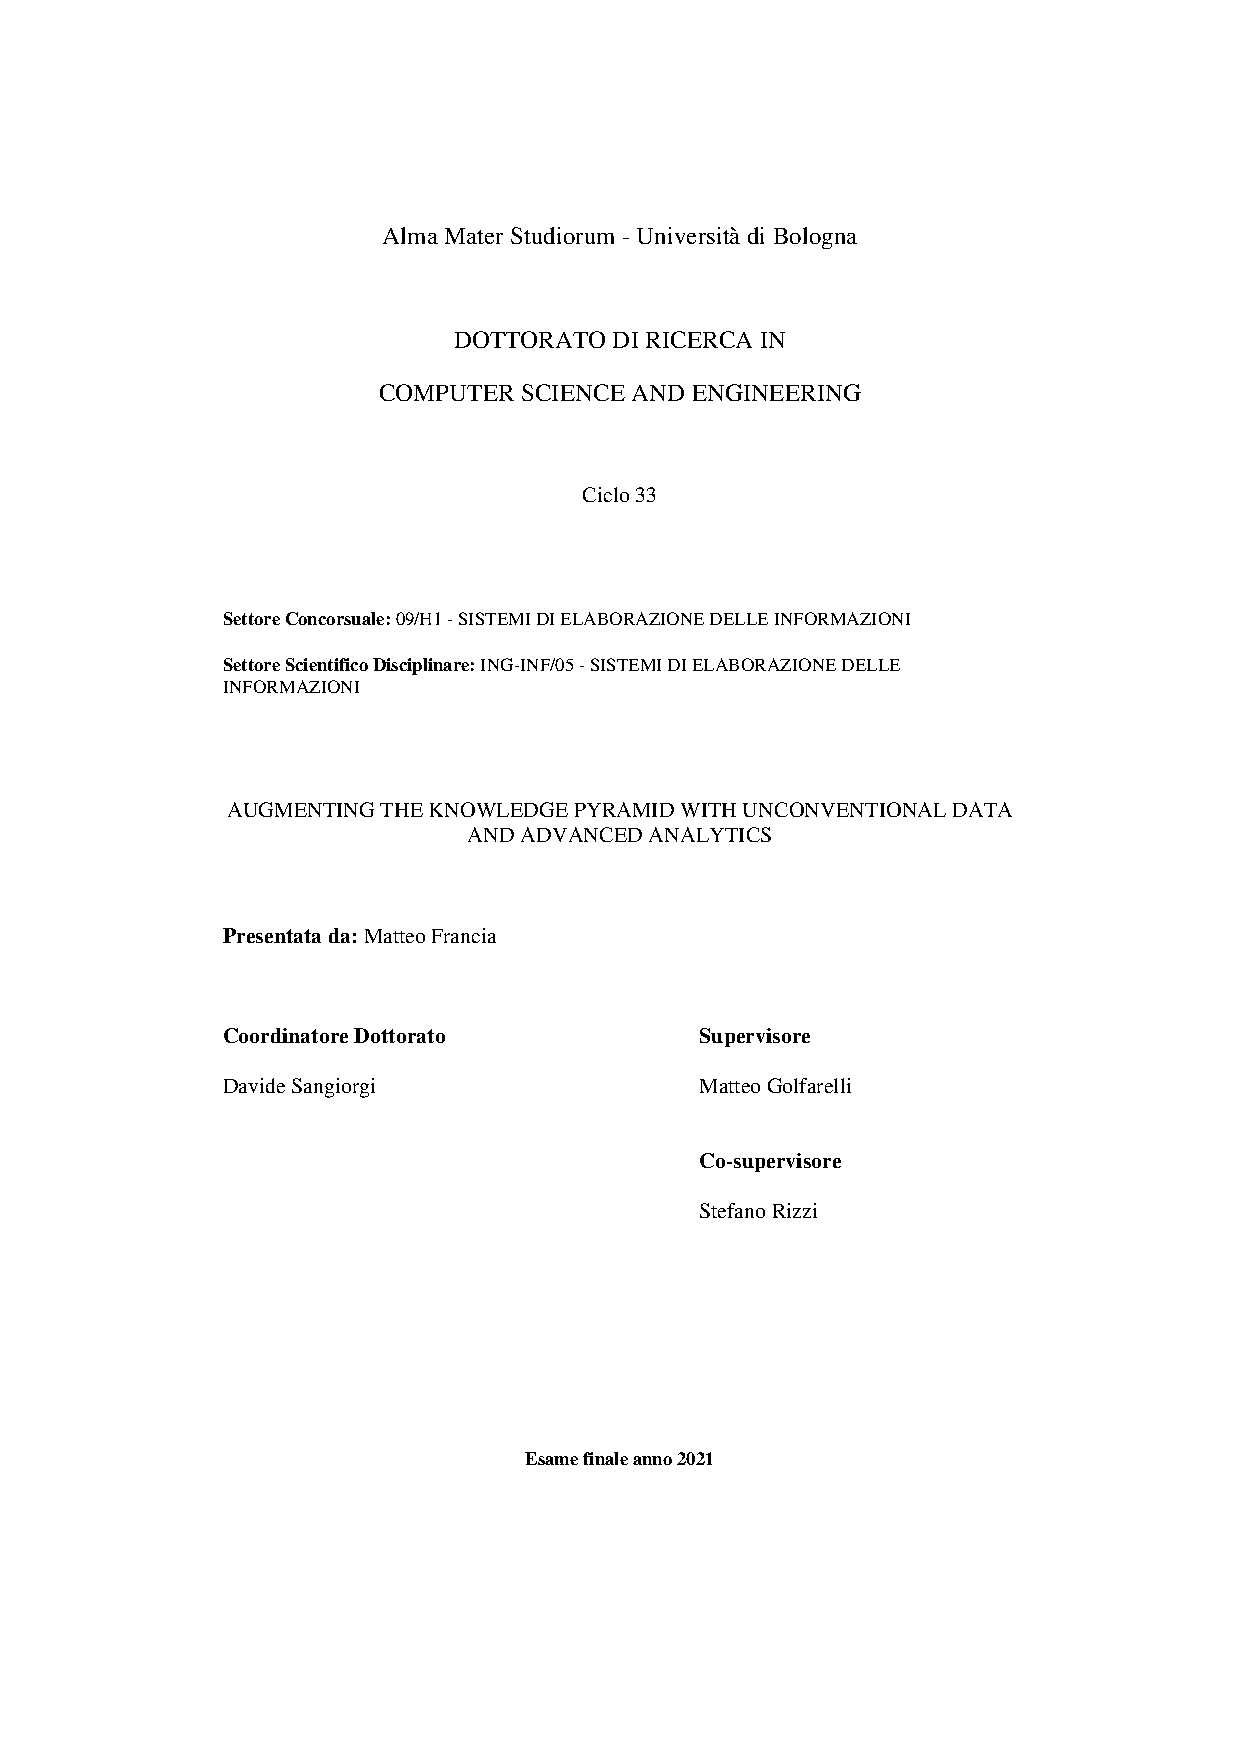
\includepdf[pages=-]{global/frontespizio.pdf}
\newpage
% 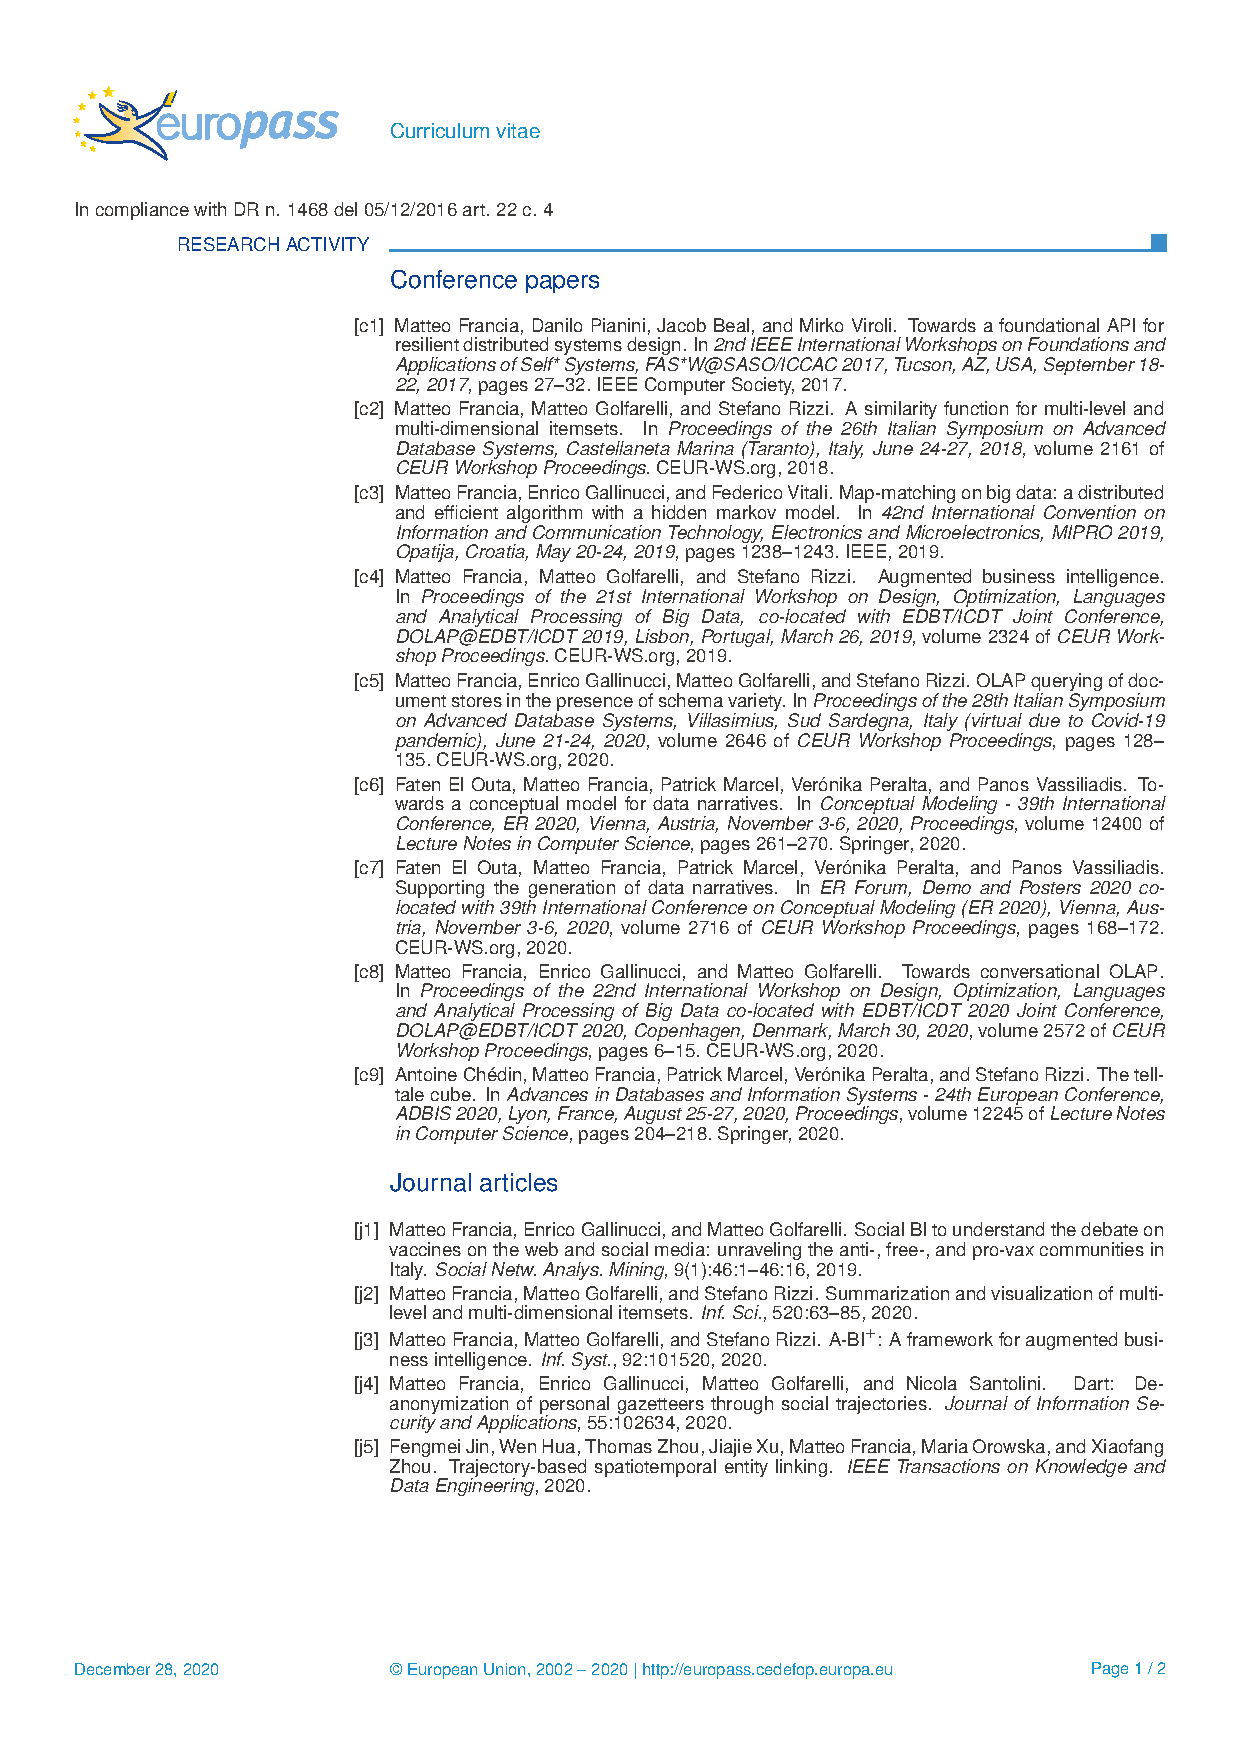
\includepdf[pages=-]{global/researchactivity.pdf}
% ******************************* Thesis Dedication ********************************
\begin{dedication}
\epigraph{\textit{
``A work of art is useless as a flower is useless.
A flower blossoms for its own joy.
We gain a moment of joy by looking at it.
That is all that is to be said about our relations to flowers.''\\
\vspace{0.5cm}
\textit{-- Oscar Wilde
% in a letter explaining ``All art is quite useless'', 1890
}}}{}
\vspace{30mm}
To Emilia.
\end{dedication}


% % ******************************* Thesis Declaration ***************************

\begin{declaration}
I hereby declare that except where specific reference is made to the work of 
others, the contents of this dissertation are original and have not been 
submitted in whole or in part for consideration for any other degree or 
qualification in this, or any other university. This dissertation is my own 
work and contains nothing which is the outcome of work done in collaboration 
with others, except as specified in the text and Acknowledgements. This 
dissertation contains fewer than 65,000 words including appendices, 
bibliography, footnotes, tables and equations and has fewer than 150 figures.
% Author and date will be inserted automatically from thesis.tex \author \degreedate
\end{declaration}
\include{global/quote}
\begin{acknowledgements}
\addcontentsline{toc}{chapter}{Acknowledgements}

Before diving into the depths of my research, I would like to acknowledge the sung and unsung heroes of this PhD journey.

\vspace{0.2cm}

% I would like to express my sincere gratitude to my advisors Prof. Matteo Golfarelli and Prof. Stefano Rizzi for their support and inspiration.
% My Ph.D. has been a joyful journey under their supervision.\\
The success of this thesis is certainly due to my research group, the business intelligence group (BIG).
First of all, I would like to thank my supervisor Prof. Matteo Golfarelli, who motivated me in the first place to start this PhD, and provided constant support and feedback.
I express my sincere gratitude to Prof. Stefano Rizzi for his priceless advice and encouragement.
I would like to thank my advisor Dr. Matteo Francia for his invaluable guidance, but also for welcoming me to the group ``so nicely''.
As to countless cups of coffee and \emph{italian passeggiate}, I thank my lab mates Dr. Enrico Gallinucci, Chiara Forresi, Manuele Pasini, Anna Giulia Leoni, Nicola Santolini, and Sterenn Roux.

\noindent At the Universitat Polit\`{e}cnica de Catalunya, Barcelona, huge thanks go to Prof. Alberto Abelló and Dr. Besim Bilalli for their inspiration and support during my Master's thesis, and throughout the whole PhD.

\noindent From Leibniz University, Hanover, I want to thank the AutoML group.
I would like to express my sincere gratitude to Prof. Marius Lindauer and Dr. Alexander Tornede, not only for the endless research insights and opportunities, but also for their kindness in welcoming me to the group.
Besides, I am grateful to have found an incredible group with which I had an amazing time.
I would like to thank Carolin Benjamins, Difan Deng, Theresa Eimer, Helena Graf, Aditya Mohan, Tim Ruhkopf, Sarah Segel, Daphne Theodorakopoulos, and Tanja Tornede.

\vspace{0.2cm}

With no doubts, I must thank my friends who both supported me during the ups and downs, and celebrated my achievements.
I would like to thank Gianluca Aguzzi,  Matteo Magnani, and Giuseppe Pisano.
I sincerely would not change anyone of you on this journey.
I would like to thank all the friends encountered during these years at the Cesena campus, especially in the Area 4.0 lab.
I believe the are not many groups having such a bond (and fun).
Especially, I would like to thank Giovanni Ciatto, Nicolas Farabegoli, Angela Cortecchia, Davide Domini, Matteo Magnini, Danilo Pianini, Martina Baiardi, Stefano Novellani, and Ruslan Shaiakhmetov.

\noindent My biggest thanks go to my mum Emilia for her never-ending support, solely a true \emph{mammone} can understand how much she means to me.
No less, I thank my father Renato and brother Yuri, for their continuous encouragement and for believing in me.

\noindent Last but not least, I would thank my partner Maria for cheering me up when ``it is not the day'', for her every-day caring, for all the fun, but -- mostly -- for always making me feel loved.

\end{acknowledgements}

\begin{abstract}
    \addcontentsline{toc}{chapter}{Abstract}

    % Riding the wave of recent groundbreaking achievements, artificial intelligence (AI) is currently the buzzword on everybody's lips and, building upon the notion of intelligence as learning, Machine Learning (ML) emerged as its pinnacle.
    % Riding the wave of recent groundbreaking achievements, artificial intelligence (AI) is currently the buzzword on everybody's lips and, addressing problems where human-crafted solutions are unfeasible, Machine Learning (ML) emerged as its pinnacle.
    % Artificial Intelligence (AI) stands as a transformative force, riding the wave of recent groundbreaking achievements, and Machine Learning (ML) emerged as its pinnacle, addressing problems where human-crafted algorithms are unfeasible and allowing algorithms to learn from historical data and discover solutions autonomously.
    % In particular, it addresses problems where human-crafted algorithms are unfeasible, allowing algorithms to learn from historical data and discover solutions autonomously.
    Riding the wave of recent groundbreaking achievements, artificial intelligence (AI) is currently the buzzword on everybody's lips and, allowing algorithms to learn from historical data, Machine Learning (ML) emerged as its pinnacle.
    The multitude of algorithms, each with unique strengths and weaknesses, highlights the absence of a universal solution and poses a challenging optimization problem.
    In response, automated machine learning (AutoML) navigates vast search spaces within minimal time constraints.
    By lowering entry barriers, AutoML emerged as promising the democratization of AI, yet facing some challenges.

    In \textbf{data-centric AI}, the discipline of systematically engineering data used to build an AI system, the challenge of configuring data pipelines is rather simple.
    We devise a methodology for building effective data pre-processing pipelines in supervised learning as well as a data-centric AutoML solution for unsupervised learning.

    In \textbf{human-centric AI}, many current AutoML tools were not built around the user but rather around algorithmic ideas, raising ethical and social bias concerns.
    % Motivated by such a mitigation call, this thesis contributes to human-centric AutoML, aiming at complementing, instead of replacing, human intelligence.
    We contribute by deploying AutoML tools aiming at complementing, instead of replacing, human intelligence.
    In particular, we provide solutions for single-objective and multi-objective optimization and showcase the challenges and potential of novel interfaces featuring large language models.

    Finally, there are application areas that rely on numerical simulators,
    % with domain experts manually configuring them through several trials and errors.
    often related to earth observations, they tend to be particularly high-impact and address important challenges such as climate change and crop life cycles.
    We commit to coupling these physical simulators with (Auto)ML solutions towards a \textbf{physics-coupled AI}.
    Specifically, in precision farming, we design a smart irrigation platform that: allows real-time monitoring of soil moisture, predicts future moisture values, and estimates water demand to schedule the irrigation.

    % starting from supervised and unsupervised learning. The former is provided with a ground
    % truth to drive the learning towards a user-specified objective function

    % for both supervised learnand unsupervised learning, a
    % towards a more human-centric AutoML process.
    % In particular,
    % This places a mitigation call a shift toward the human-centric paradigm
    % Enabling human intervention, translating into the need for a shift toward the human-centric paradigm.
    % pushed towards a more human-centric AutoML process aimed at complementing, instead of replacing, human intelligence.

\end{abstract}
\tableofcontents
% \listoffigures
% \listoftables
% \printnomenclature%[3em]

% ******************************** Main Matter *********************************
\mainmatter
\sloppy
% \chapter{The Knowledge Pyramid}
\begin{figure}[t]
    \centering
    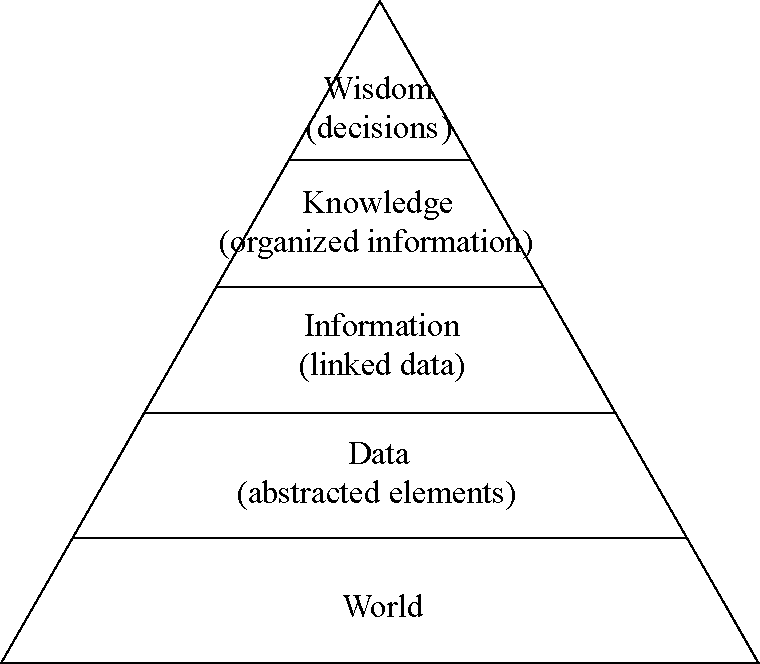
\includegraphics[scale=.7]{global/DIKW.pdf}
    \caption{The ``knowledge pyramid'' (also known as the ``Data Information Knowledge Wisdom pyramid'' or ``knowledge hierarchy''; adapted from \cite{DBLP:journals/oir/Stuart15b}).}
    \label{fig:dikw}
\end{figure}

Data science extracts actionable insights from raw data \cite{kelleher2018data}. The data transformation process is usually abstracted in the ``knowledge pyramid'' (also known as the ``Data Information Knowledge Wisdom pyramid'' or ``knowledge hierarchy''; \Cref{fig:dikw}), where data (i.e., symbols) are collected through measurements taken from the real world; information is processed and linked data that it is meaningful to scientists; knowledge is interpreted, understood, and organized information; and wisdom is knowledge in action. Climbing the pyramid is not a straightforward path and requires the iterative exploration and preparation of data so that patterns can be extracted, evaluated, and later deployed into models supporting effective decisions. 

Analytic applications strive to extract knowledge from data fueled by pervasive systems \cite{8423172}, where any device can be turned into a sensor leading to a huge volume and variety of available data \cite{vitali2021crop}. These \textit{unconventional}\footnote{We consider \textit{conventional} the data collected by operational databases, ERP (enterprise resource planning), and CRM (customer relationship management) enterprise systems} data (i.e., unstructured and non-relational data) have impacted on business intelligence (BI)---the discipline providing strategies and technologies to transform data into decision-making information---leading to BI 2.0, where decisions are drawn \textit{not only} on the data owned by the organization. Indeed, bigger data volumes lead to a holistic view of historic and current trends; higher data velocities ground decisions in continuously updated data, and broader data varieties provide many nuances of the matter at hand \cite{IBM4V}. On the one hand, volume and variety hinder the management, the integration, and the analysis of the collected data (from ``World'' to ``Data'' in \Cref{fig:dikw}), since each instance of unstructured data might have a different structure. This requires ad-hoc techniques for different data types (e.g., social networks \cite{DBLP:journals/snam/FranciaGG19} or sensor data \cite{DBLP:conf/mipro/FranciaGV19}). On the other hand, high availability has attracted scientists with no expertise in computer science or data engineering, requiring novel paradigms to support the ``Data''-to-``Knowledge''
%\footnote{Since ``wisdom'' is related to the \textit{application} of knowledge \cite{8423172}---besides no strict definition is given in the literature---we address the transformation of raw data into knowledge (i.e., patterns extracted with mining/machine learning models).} 
transformation with a higher abstraction level than formal programming languages (e.g., through graphical metaphors, recommender systems, or automatic transformation pipelines). Additionally, availability has enabled pervasive analyses, allowing data scientists to access data in hand-free contexts involving augmented reality and smart assistants.

While investigating these challenges, this thesis evolves into two parts.

\begin{figure}[t]
    \centering
    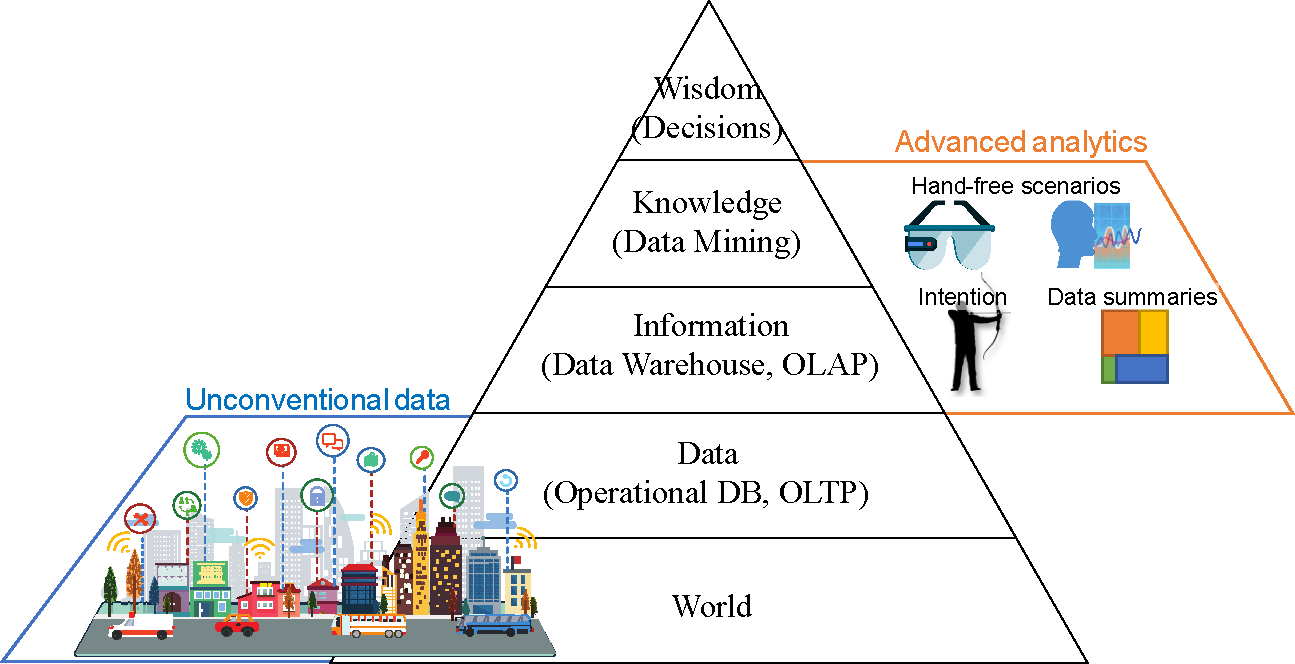
\includegraphics[scale=.65]{global/augmenting.pdf}
    \caption{Augmenting the knowledge pyramid with unconventional data (left) and advanced analytics (right).}
    \label{fig:aug}
\end{figure}

\paragraph{\Cref{part:trajectory}: Unconventional Data.}
Sensing provides real-time data upon which ``contextual'' decisions---ranging from user-centric to societal problems---are based. This includes data collected from human and technological assets (e.g., sensor or mobile networks), which are analyzed to monitor and manage urban and rural areas. Sensor data are highly available due to the growth of Internet of Things devices, have variable content, and their value comes from historic trends that range from hours to years \cite{kelleher2018data}. Such volume and variety demand for augmenting the knowledge pyramid with novel and scalable techniques for different data types (\Cref{fig:aug}). In urban mobility, spatiotemporal data (i.e., temporal sequences of spatial locations traced by moving objects and sampled through global or relative positioning sensors) are collected and processed for the sake of traffic analysis and forecasting, clustering of objects moving in similar paths, and habits profiling. Spatiotemporal data are challenging because of their uncertain, sparse, and multiresolution nature \cite{DBLP:journals/cacm/GilPBBBBCEGHHHK19}. Also, due to the number of moving objects (e.g., mobile devices, cars, taxis, and public transport in a metropolitan area) and to the sampling rate of positioning sensors (e.g., from minutes to seconds), mining mobility data easily scale up to big-data problems that require big-data solutions, hence introducing %a 
new business opportunities
% to analyze and extract information from data 
that were previously ignored because of technology limitations. Besides the valuable knowledge, due to high uniqueness \cite{DeMontjoye2013} and sensitivity (e.g., home and work locations), trajectory data expose individuals to privacy violations, demanding for ad-hoc techniques to (de-)anonymize historical trajectory datasets. In this direction, \Cref{part:trajectory} focuses on trajectory data and on the privacy implications of the publication of long-term mobility datasets.

\paragraph{\Cref{part:olap}: Advanced Analytics.}
Since the introduction of the relational model in the '70s, users used relational queries (e.g., SQL queries) to retrieve data collected in operational databases. This requires a good comprehension of programming languages and database management systems. Later, more user-friendly abstractions and tools provided a simpler view of the data, hiding the complexity of the underlying databases \cite{DBLP:journals/is/VassiliadisMR19} and transitioning from static (repetitive) workloads involving a few records (On-Line Transaction Processing, OLTP) to dynamic workloads (On-Line Analytical Processing, OLAP, and On-Line Analytical Mining, OLAM) involving a huge amount of records (\Cref{fig:aug}). The spread of data and analytical tools at hand has brought an increasing participation of data scientists with high competence in the business domain but low competence in computer science and data engineering \cite{DBLP:journals/is/VassiliadisMR19}. Indeed, data science emerged as an amalgamation of domain expertise with disciplines such as statistics, data mining, and databases \cite{vanderAalst2016}. Such amalgamation has brought challenges not only concerning big data volumes but also in terms of the increasing complexity and interdisciplinarity of the analytic questions. Enabling an effective participation in data science requires the investigation of user-centric paradigms supporting analytical querying and making knowledge extraction more accessible. Data scientists can benefit from proactive systems that ``understand'' the tasks at hand, make recommendations, and generate effective visualizations \cite{DBLP:journals/cacm/GilPBBBBCEGHHHK19}. For instance, in the digital twin scenario \cite{tao2018digital} where physical entities are mapped into a digital world, the synergy of personal assistants and augmented reality lacks analytic capabilities. Additionally, limited attention has been devoted to providing analytical reports that can be useful to let the user compare the current behavior of the visualized objects with their historical behavior. To this end, unconventional data sources, such as smart glasses and wearable devices, can be accessed by personal assistants (e.g., recommender systems) to address users' needs \cite{DBLP:conf/ictir/BahrainianC17}. Data scientists can interact with personal assistants through natural language interfaces which provide a higher abstraction level than formal queries and programming languages. In this direction, \Cref{part:olap} focuses on supporting data scientists with higher analytic abstractions than formal queries also in scenarios entailing pervasive data access. 



\chapter{Research Path Overview}
\label{chap:intro}

Artificial intelligence (AI) is currently the buzzword on everybody's lips.
Riding the wave of recent groundbreaking achievements, from self-driving cars \cite{badue2021self} to intelligent chatbots \cite{adamopoulou2020chatbots}, AI is transforming industries and reshaping our daily lives.
Several interpretations and definitions have been provided over the years, yet the seminal perspective given by the Turing test \cite{turing1980computing} is still one worth mentioning.
\begin{definition}[Artificial Intelligence \cite{turing1980computing}]
A machine that shows intelligence indistinguishable from that of human beings is qualified to be labeled as artificial intelligence.
\end{definition}
This translates into understanding what falls under the umbrella of \textit{intelligence}, which is defined differently across the research areas as reasoning, planning, and learning.
\begin{definition}[Machine Learning \cite{samuel2000some}]
A machine with the ability to learn without being explicitly programmed.
\end{definition}
Building upon the notion of intelligence as learning, i.e. Machine Learning (ML), emerged as the pinnacle of AI due to its disruptive advancements.
At its core, ML aims at addressing problems for which the development of algorithms by humans is not feasible, because the algorithm itself is either not known or cost-prohibitive.
Examples include face recognition, fraud detection, sale forecasting, and object ranking.
The problems are solved instead by letting the algorithms (e.g., neural networks \cite{bishop1994neural}) \textit{discover their own solutions}: they perform a training process atop a sample of historical data, borrowing techniques from disciplines such as numerical analysis, statistics, and information theory.
The training process consists of fitting internal parameters (e.g., weights and bias) and providing practitioners with a model.
In this context, we can hence define an \textit{AI system} as the (software) solution that deploys an ML model specific for the problem at hand i.e., ready to ingest new data and tackle it.

There exists a plethora of different algorithms solving the same problem with different strengths and weaknesses, confirming theoretical results proving that there is \textit{no silver bullet} \cite{kerschke2019automated}---no algorithm dominates all others in all respects.
Besides, algorithms often expose some hyperparameters controlling the learning behavior (e.g., learning rate).
To unleash the full potential of ML, practitioners have to carefully tune such hyperparameters but get easily overwhelmed by the showcased problem of combined algorithm selection and hyperparameter (CASH) optimization.

Automated machine learning (AutoML) demonstrates to play a crucial role in this landscape by tackling the CASH problem and, going beyond, by handling ever-larger search spaces in surprisingly small time budgets \cite{thornton2013auto, olson2016tpot, auto_sklearn}.
Remarkable milestones include bayesian optimization (BO) to explore promising configurations based on prior evaluations,
meta-learning (i.e., learning atop learning) to warm-start BO (i.e., to boost the convergence process) by suggesting configurations that worked well in previous similar cases, and multi-fidelity methods to partially evaluate time-consuming configurations.
By lowering the barrier of access, AutoML emerged as promising for the democratization of AI, i.e. making it accessible to both experts and non-experts alike.
Yet, when it comes to real-case scenarios, the journey of
delivering AI systems is riddled with challenges.

\begin{figure}
    \centering
    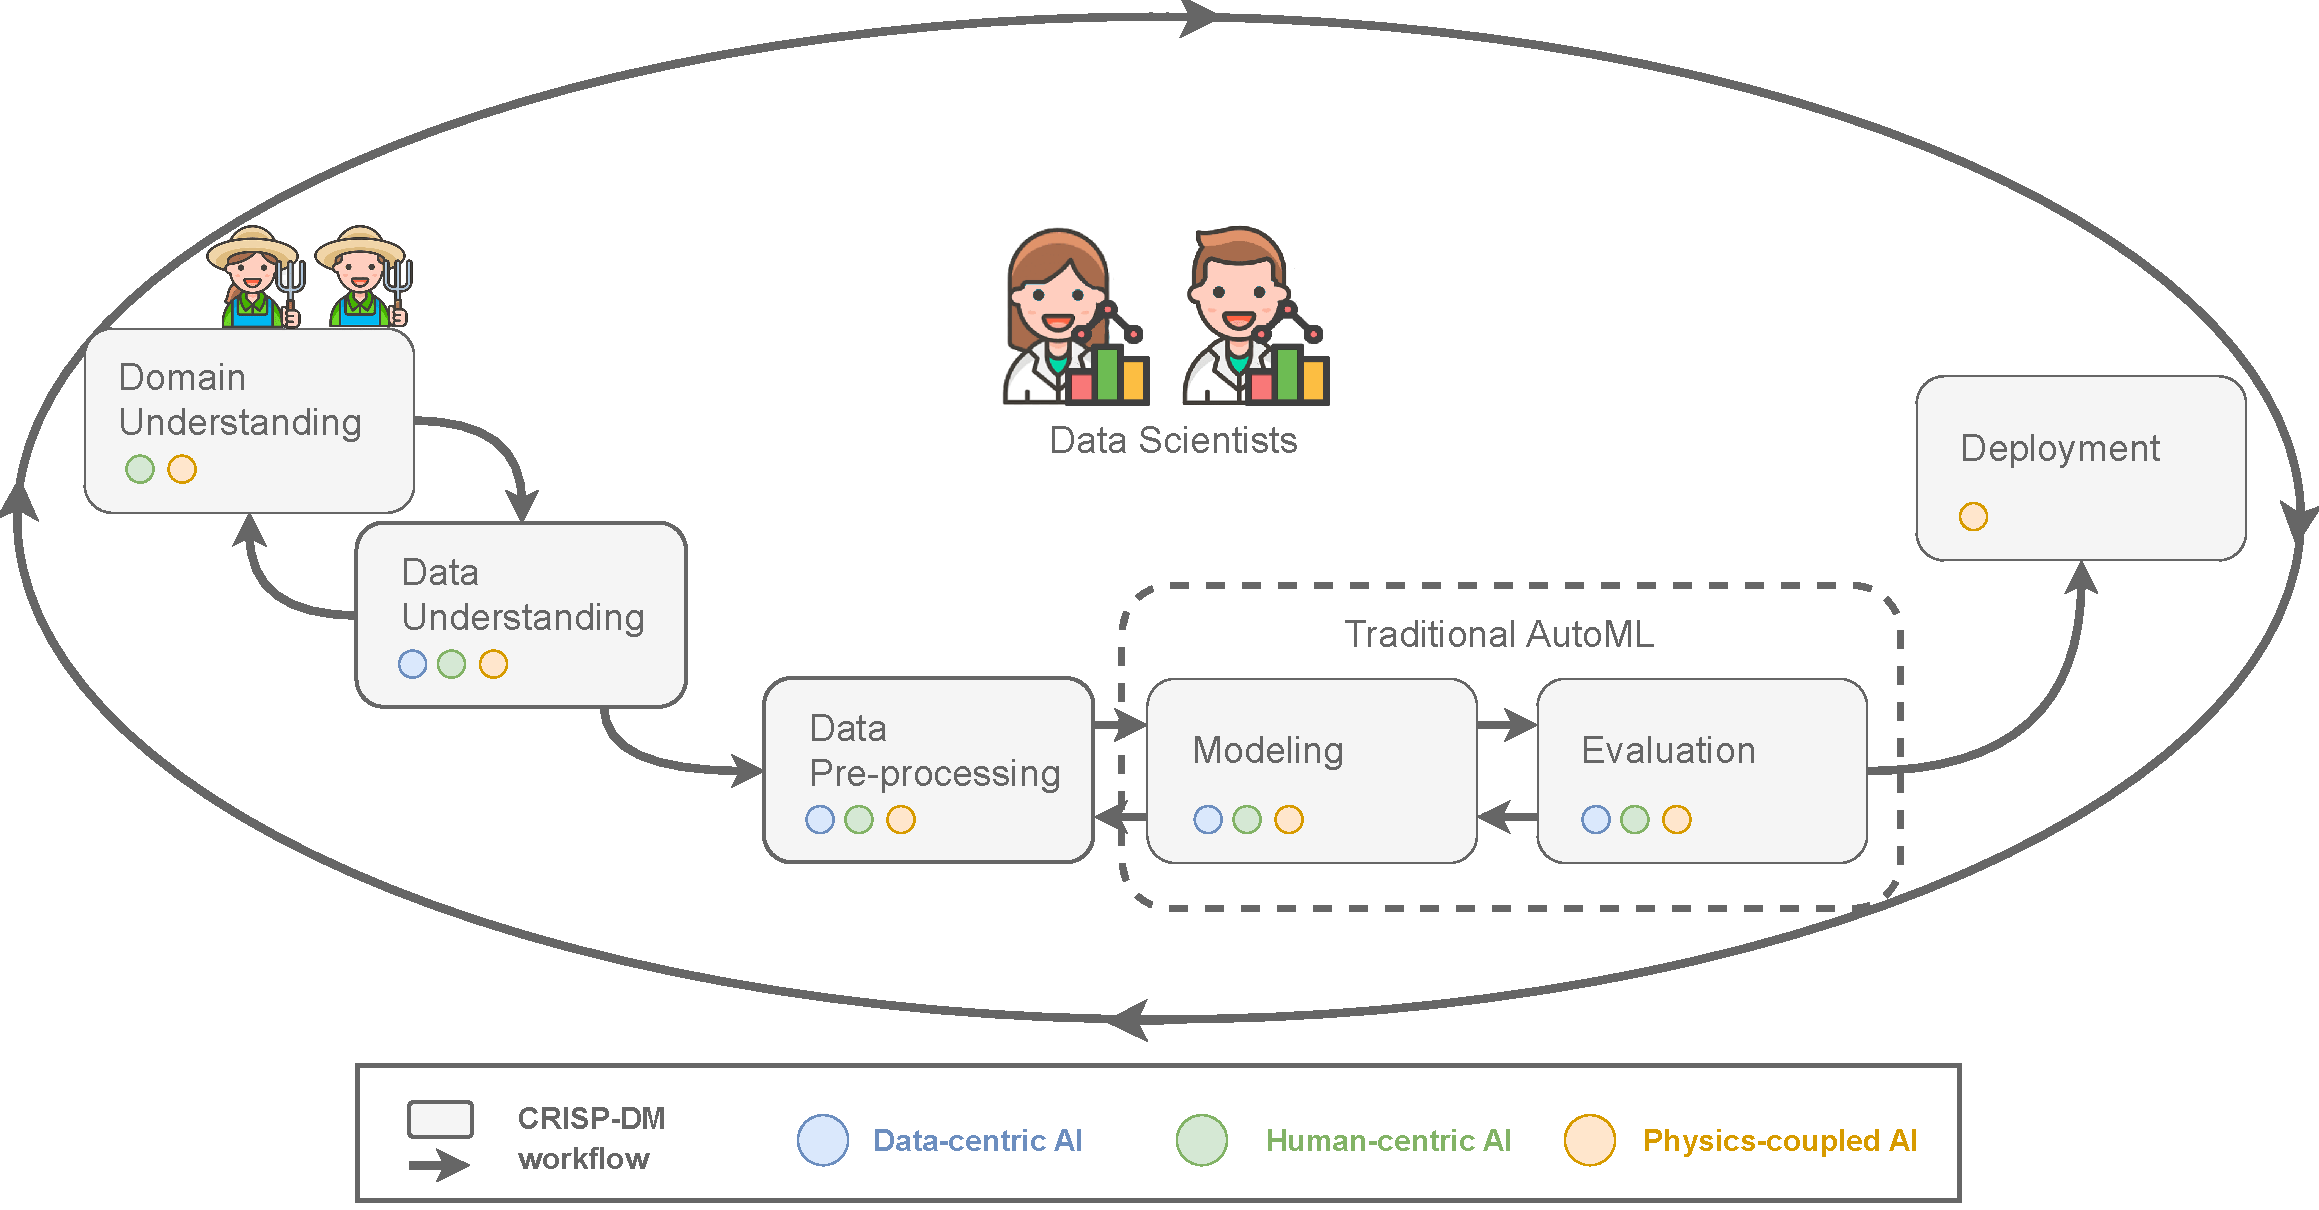
\includegraphics[width=1\textwidth]{chapters/introduction/img/contribution_overview.pdf}
    \caption{Contirbution overview.}
    \label{fig:contribution}
\end{figure}

Let us quickly overview the end-to-end process.
The main character is usually the data scientist, a specialist in machine learning and data analysis, which leverages a process model to translate the \textit{knowledge} about the problem into \textit{ML constraints} and deploy the system.
The cross-industry standard process for data mining (CRISP-DM) \cite{wirth2000crisp} is considered the open standard and we will take it as a reference in the whole thesis.
Given the numerous skills expected by data scientists,
their numbers fall short of the needs,
leading domain experts to carry out such a process.
For the sake of simplicity, we keep these two roles separated.
\textbf{Domain} and \textbf{data understanding} entail domain experts and the data scientist working in close cooperation to explore constraints and study available data, respectively.
These stages might be repeated many times until the data scientists are satisfied with the acquired knowledge.
Follows the iterative investigation of different solutions throughout \textbf{data pre-processing}, \textbf{modelling}, and \textbf{evaluation}.
Data pre-processing and modelling are conducted to build a data pipeline and train an ML algorithm, respectively.
More in detail, a series of pre-processing transformations shape the data so that the ML algorithm can output the best model.
Then, evaluation offers a way to measure the performance and the process can conclude with the \textbf{deployment} of the AI system, including the implementation of the running environment.

\Cref{fig:contribution} shows the CRISP-DM process model and the research areas we focus on.
Specifically, according to challenges that are addressed: data-centric, human-centric, and physics-aware AI.
While \Cref{chap:background} provides the necessary background, the remaining of the thesis evolves in the corresponding three parts.

\section*{Part I: Data-centric AI}

During the past few decades, most of the efforts in AI were focused on improving ML algorithms, leading to numerous groundbreaking achievements.
In many applications, modelling is considered the solved part of the puzzle and the vast majority of the time is spent on improving the data.
Data-centric AI is the discipline of systematically engineering data used to build an AI system, yet the challenge of configuring data pipelines is rather simple.
A combinatorial space has to be explored, entailing ad-hoc pre-processing for the algorithm at hand, and constraints within data, transformations, and algorithms exacerbate the problem at hand.
While AutoML traditionally neglected data quality and pre-processing, there is an untapped potential to contribute to this research area.
Indeed, given the huge combinatorial space, AutoML can help in designing efficient AI systems with a meticulous focus on data.

In \Cref{part:data-centric}, we devise data-centric solutions for the main categories of ML i.e., supervised and unsupervised learning.
Specifically, we focus on the following challenges and contributions.

\subsection*{Effective Data-preprocessing Pipelines in Supervised Learning}

\paragraph{Challenge} Data pre-processing
encompasses a broad range of transformations that span from correcting errors to selecting the most relevant features for the modelling phase.
In supervised learning, during modelling, the ML algorithm is provided with ground truth to drive the learning toward a user-specified objective function.
There is no clear evidence, or rules defined, on how these transformations impact the final results of the process.
Besides, the problem is exacerbated when transformations can be combined into pipelines.
Data scientists cannot easily foresee the overall impact, requiring a method to discriminate between them and hence find the most relevant ones for their study at hand.

\paragraph{Contribution} In \Cref{data-centric-chap:supervised}, we study the impact of transformations in general, and the impact of transformations when combined together into pipelines.
We make use of rules that enable the construction of prototypes (i.e., ordered series of transformations) and, once found, these prototypes can be tuned -- similarly to algorithm hyperparameters -- using AutoML.
The optimization of our effective prototypes provides results that compared to an exhaustive search, get 90\% of the predictive accuracy in the median, but with a time cost that is 24 times smaller.

\subsection*{Exploring Clustering Pipelines via AutoML and Diversification}


\paragraph{Challenge}
AutoML has witnessed effective applications in the field of supervised learning -- mainly in classification tasks --  where the goal is to find the best ML pipeline when a ground truth is available.
This is not the case for unsupervised tasks that are by nature exploratory and they are performed to unveil hidden insights.
Since there is no right result, analyzing different configurations is more important than returning the best-performing one.
When it comes to exploratory unsupervised tasks -- such as cluster analysis --  different facets of the datasets could be interesting for the data scientist; for instance, data items can be effectively grouped together in different subspaces of features.

\paragraph{Contribution}
In \Cref{data-centric-chap:unsupervised}, we design a framework that explores and returns a dashboard of both relevant and diverse clusterings via AutoML and diversification.
AutoML ensures that the explored pipelines for cluster analysis (including pre-processing steps) compute good clusterings.
Then, diversification selects, out of the explored clusterings, the ones conveying different clues to the data scientists.

\section*{Part II: Human-centric AI}

The original promise of AutoML was to automate certain ML tasks to a significant extent, thereby democratizing it and enabling non-experts to apply it in their respective domains.
However, despite their success, many current AutoML tools were -- yet another time -- not built around the user but rather around algorithmic ideas.
The stacking of complex mechanisms on top of each other unavoidably led to a less understanding of the process -- even by ML experts -- and allowing for very limited interaction.
Parts of the community have hence pushed towards a more human-centric AutoML process aimed at complementing, instead of replacing, human intelligence.
Besides, motivated by ethical concerns and social bias issues arising at each step of the ML process, this approach becomes even imperative in such a mitigating call nowadays.
By placing the user back in the loop, we let the user to revise and supervise the entire process, ensuring fairness, transparency, and ethical compliance.

In \Cref{part:human-centric}, we focus on the following challenges and contributions.

\subsection*{Human-centric AutoML via Structured Argumentation}

\paragraph{Challenge} In the last decade, we have witnessed exponential growth in both the complexity and the number of ML techniques; leveraging such techniques to solve real-case problems has become difficult for Data Scientists.
Automated Machine Learning (AutoML) tools have been devised to alleviate this task, but easily became as complex as the ML techniques themselves---with Data Scientists losing control over the process.

\paragraph{Contribution} In \Cref{human-centric-chap:hamlet}, we design HAMLET (Human-centric AutoMl via Logic and argumEnTation), a framework that helps data scientists to redeem their centrality.
HAMLET enables data scientists to express ML constraints in a uniform human- and machine-readable medium.
User-defined constraints are interpreted to drive the exploration of ML pipelines (i.e., data pre-processing transformations shape the data so that the ML task can be performed at its best).
AutoML retrieves the most performing pipeline instance, and finally, new constraints are learned and integrated through Logic and Argumentation.
By doing so, HAMLET not only allows easy exploitation of the knowledge acquired at each iteration but also enables its continuous revision via the AutoML tool and the collaboration of both Data Scientists and domain experts.


\subsection*{Interactive Hyperparameter Optimization in Multi-Objective Problems via Preference Learning}


\paragraph{Challenge} Hyperparameter optimization (HPO) is important to leverage the full potential of machine learning (ML).
In practice, users are often interested in multi-objective (MO) problems, i.e., optimizing potentially conflicting objectives, like accuracy and energy consumption.
To tackle this, the vast majority of MO-ML algorithms return a Pareto front of non-dominated machine learning models to the user.
Optimizing the hyperparameters of such algorithms is non-trivial as evaluating a hyperparameter configuration entails evaluating the quality of the resulting Pareto front.
In literature, there are known indicators that assess the quality of a Pareto front (e.g., hypervolume, R2) by quantifying different properties (e.g., volume, proximity to a reference point).
However, choosing the indicator that leads to the desired Pareto front might be a hard task for a user.

\paragraph{Contribution} In \Cref{human-centric-chap:moo}, we propose a human-centric interactive HPO approach tailored towards multi-objective ML leveraging preference learning to extract desiderata from users that guide the optimization.
Instead of relying on the user guessing the most suitable indicator for their needs, our approach automatically learns an appropriate indicator.
Concretely, we leverage pairwise comparisons of distinct Pareto fronts to learn such an appropriate quality indicator.
Then, we optimize the hyperparameters of the underlying MO-ML algorithm towards this learned indicator using a state-of-the-art HPO approach.
In an experimental study targeting the environmental impact of ML, we demonstrate that our approach leads to substantially better Pareto fronts compared to optimizing based on a wrong indicator pre-selected by the user, and performs comparable in the case of an advanced user knowing which indicator to pick.


\subsection*{AutoML in the Age of Large Language Models: Current Challenges, Future Opportunities and Risks}

\paragraph{Motivation} The fields of both Natural Language Processing (NLP) and Automated Machine Learning (AutoML) have achieved remarkable results over the past years.
In NLP, especially Large Language Models (LLMs) have experienced a rapid series of breakthroughs very recently.
We envision that the two fields can radically push the boundaries of each other through tight integration.

\paragraph{Contribution} To showcase this vision, in \Cref{human-centric-chap:llm} we explore the potential of a symbiotic relationship between AutoML and LLMs, shedding light on how they can benefit each other.
In particular, we investigate both the opportunities to enhance AutoML approaches with LLMs from different perspectives and the challenges of leveraging AutoML to further improve LLMs.
To this end, we survey existing work, and we critically assess risks.
We strongly believe that the integration of the two fields has the potential to disrupt both fields, NLP and AutoML.
By highlighting conceivable synergies, but also risks, we aim to foster further exploration at the intersection of AutoML and LLMs.

\section*{Part III: Physics-coupled AI}

As application areas go, there are domains in which ML models are not yet widespread.
Usually related to earth observations, the deployed applications tend to be particularly high-impact, trying to mitigate challenges such as climate change by delivering (more) eco-friendly systems.
Examples include weather forecasts and crop life-cycle management.
Domain experts leverage their knowledge to tune process-based models -- i.e., mathematical models that encode well-known physical laws -- and deliver forecasts and analyses.
However, this process faces several challenges.
The non-existence of universal well-defined practices translates to several trials and errors, with domain experts manually configuring the simulator parameters until an acceptable solution is found.
Yet, as variables involved in physics phenomena are subject to constant change, such process-based solution must undergo periodic (re-)calibration.
Besides, with the torrent of remotely sensed data available today, opportunities to integrate real-time observations in predictive models have emerged that traditional methods are not equipped to handle.
This is where advances in AI can push forward to enhance our understanding, provide support and, if necessary, steer the course of resolving global concerns to a more favorable future.
For instance, ML models exhibit singular performance in adapting themselves to handle scenarios different from the one they were trained on (e.g., fine-tuning of network parameters) and AutoML can significantly impact in automating several stages (e.g., tuning simulators and ML models).

In \Cref{part:physics-aware}, we focus on precision farming, which plays a pivotal role in addressing water wastage and improving crop efficiency.
Specifically, we provide the necessary background and related works in \Cref{physics-aware-chap:background} and, in the remaining, we commit to the following challenges and contributions.


\subsection*{Multi-Sensor Profiling for Precision Soil Moisture Monitoring}


\paragraph{Challenge}
In a contest of climate change and increasing world population, the optimization of watering and crop performance is of utmost importance to assure food security and quality.
For this reason, the need for robust methods of soil moisture monitoring has never been clearer.
% Controlling soil moisture is crucial in optimizing watering and crop performance.
Yet, traditional monitoring systems rely on a single sensor or on a column of sensors that do not allow farmers to properly capture soil moisture dynamics in the soil volume occupied by roots.


\paragraph{Contribution} In \Cref{physics-aware-chap:pluto}, we propose PLUTO, an original approach that builds fine-grained 2D and 3D soil moisture profiles by relying on a grid of sensors.
Profiles are computed using both process-based and machine-learning approaches.
Besides the technical description of the approach, this chapter reports a set of original visualizations and a large set of tests computed, over two years, on real Kiwi orchards.
PLUTO proved to largely overcome the accuracy of profiles obtained with traditional sensor layouts.
Considering that the cost of sensors is progressively decreasing, PLUTO provides a cost-effective, operative, and precise solution to moisture monitoring.


\subsection*{Enhancing Process-Based Models for Precision Soil Moisture Forecasting}

\paragraph{Challenge}
% In a contest of climate change and increasing world population, the optimization of agricultural inputs such as water and fertilizer is of utmost importance to assure food security and quality.
Optimization watering and crop performance is a complex real-case problem, and several solutions have been proposed.
% While soil moisture monitoring is just one side of the coin, soil moisture forecasting has demonstrated itself particularly effective.
Even machine learning models leverage process-based models to generate synthetic data and deploy forecast systems.
% the need for robust methods of agricultural modeling and forecasting has never been clearer.
Yet, the accuracy and precision of agricultural modeling and forecasting remain limited by current tools and methods.

\paragraph{Contribution} In \Cref{physics-aware-chap:orchard}, to overcome the limitations of process-based models, we are proposing an integrated system coupling a three-dimensional numerical model with an assimilation procedure that exploits a bi-dimensional sensor grid.
The system is capable of auto-tuning its parameters on a specific soil and of providing a very precise forecast that can support precision watering policies on a weekly horizon.
A large set of tests has been carried out on an experimental farm in Northern Italy where Kiwifruit is cultivated.
Besides accuracy, tests proved the robustness of the system even in the presence of a limited set of examples for parameter auto-tuning.
This makes our approach concretely applicable in real-world settings.


% \subsection*{Adaptive Soil Moisture Forecasting for Long-Term Irrigation Planning}


% \paragraph{Challenge} $\dots$


% \paragraph{Contribution} In \Cref{physics-aware-chap:forecasting}, $\dots$

\chapter{Background}
\label{chap:background}

Alan Turing defines the field of AI in cognitive terms \cite{turing1980computing}, raising the question of whether machines can show intelligence, and along this line Arthur Samuel defines ML \cite{samuel2000some}, building upon the notion of intelligence as learning.
A more formal definition is provided by Tom M. Mitchell \cite{mitchell1997machine}, who delineates the behavior of algorithms studied in machine learning and introduces the concepts of \textit{task} and \textit{experience}.
\begin{definition}[Machine Learning \cite{mitchell1997machine}]
    A computer program is said to learn in some class of tasks, with respect to a performance measure, if its performance improves with experience.
\end{definition}
Notably, the formalization of experience is contingent upon the task to address, which is crucial because determines what the ML algorithm can observe and, in turn, how it operates.
Specifically, the literature identifies three different ML tasks: \textit{supervised}, \textit{unsupervised}, and \textit{reinforcement learning}.

\paragraph{Supervised learning} This is the kind of learning studied in most current research in the ML field. The algorithm is provided with a sample of data describing scenarios that have been \textit{experienced} in the past along with the corresponding \textit{ground truth}---i.e., values that indicate the correct outcomes.
The goal consists of finding a \textit{function} that maps samples to outcomes so that the next unseen scenarios can be labeled correctly.


\paragraph{Unupervised learning}
Here, the samples come with no ground truth available.
The algorithm has to guess the outcome by uncovering hidden insights or patterns, investigating different partitionings, or estimating density distributions within the data.
Unsupervised tasks are inherently exploratory in nature and are often employed in data mining to provide explanations for the given scenarios or even to summarize them.

\paragraph{Reinforcement Learning}
Standing on the edge of the ML landscape, it has been categorized as the learning that differentiates the most from ``classical'' tasks \cite{sutton2018reinforcement}.
Here the experience is not sampled and fed to the algorithm but rather comes from interactions with an environment.
The algorithm learns by making decisions and receiving feedback based on its actions, allowing it to adapt its behavior over time.\\

\todo{Qua c'è da menzionare che infatti automatizzare RL, in letteratura, prende il nome di AutoRL mentre noi facciamo AutoML.}
This thesis focuses on supervised and unsupervised learning.
Particularly in this chapter, \Cref{automl-background-sec:ml} introduces the building blocks such as dataset, algorithm, and hyperparameter;
\Cref{automl-background-sec:automl} formalizes the problems tackled by automated machine learning (AutoML), up to the combined algorithm selection and hyperparameter optimization; and finally, \Cref{automl-background-sec:pipelines} details the challenges in optimizing thorough ML pipelines.

\section{Machine Learning}\label{automl-background-sec:ml}

At the core of each and every task lies the data, serving as the essential fuel for the learning process because providing the means to observe the real world.
Specifically in ML, we refer to a dataset $\altmathcal{D}$ as a sample of data from which it is possible to learn that experience of interest.

\begin{definition}[Dataset]\label{def:dataset}
    A \textit{dataset} $\altmathcal{D}$ is a collection of data points $X$, with corresponding space $\altmathcal{X}$.
    According to the task $T$, the dataset may include the ground truth $Y$ within its corresponding space $\altmathcal{Y}$ (supervised) or not (unsupervised).
    \begin{equation*}\label{eq:dataset}
        \altmathcal{D} = \left\lbrace\,
        (d_i)_{i=1}^N  \quad \begin{array}{|@{}l@{}l@{\quad}l@{}}
            \quad d_i = (\pmb{x}_i, y_i) & \in \mathbb{D} \subset \altmathcal{X} \times \altmathcal{Y} & \text{{if }} T = \text{{supervised}} \\
            \quad d_i = \pmb{x}_i & \in \mathbb{D} \subset \altmathcal{X} & \text{{if }} T = \text{{unsupervised}}
        \end{array}
        \right\rbrace
    \end{equation*}
\end{definition}

Intuitively, a dataset resembles a structured table where each row represents a unique instance $x \in X$ characterized by specific features in their domain $\altmathcal{X}$.
The features, denoted by the columns, describe the diverse factors or characteristics influencing a particular outcome $Y$ in its domain $\altmathcal{Y}$.
While in supervised learning the ground truth is provided with the aim of understanding the hidden relationships between features and corresponding outcomes, in supervised tasks, the most appropriate outcome has to be found by discovering patterns within the data.

\begin{example}[Iris dataset \cite{iris}]\label{ex:dataset}
    The iris dataset contains $150$ instances of flowers ($X$) under four features in cm ($\altmathcal{X} \subset \mathbb{R}^4$): sepal length, sepal width, petal length, and petal width.
    The data have been collected to quantify the morphologic variation within the Iris species ($Y$), which can assume the following $3$ classes ($\altmathcal{Y}$): Iris setosa, Iris virginica and Iris versicolor.
    \begin{table}[!h]
        \centering
        \begin{tabular}{llll|l}
            \hline
            Sepal length & Sepal width & Petal length & Petal width & Class \\ \hline
            % $5.1$ & $3.5$ & $1.4$ & $0.2$ & Iris-setosa \\
            $4.9$ & $3.0$ & $1.4$ & $0.2$ & Iris-setosa \\
            % $7.0$ & $3.2$ & $4.7$ & $1.4$ & Iris-versicolor \\
            $6.4$ & $3.2$ & $4.5$ & $1.5$ & Iris-versicolor \\
            % $6.3$ & $3.3$ & $6.0$ & $2.5$ & Iris-virginica \\
            $5.8$ & $2.7$ & $5.1$ & $1.9$ & Iris-virginica \\ \hline
            \
        \end{tabular}
        \caption{Example tuples from the Iris dataset.}
        \label{tbl:iris}
    \end{table}

    \noindent This dataset is also used in unsupervised learning tasks by discarding the class attribute, yet the data only contains two clusters with rather obvious separation.
\end{example}

% The aim is to discover the hidden relationships between inputs $X$ and outputs $Y$, hence learning a function $f: \altmathcal{X} \rightarrow \altmathcal{Y}$.
% Despite the task,
The ultimate goal is learning a function $f: \altmathcal{X} \rightarrow \altmathcal{Y}$.
A (machine) learning \textit{algorithm} $A$ leverages data points in $\altmathcal{D}$ to estimate such a function $f$, which is expressed via a vector of \textit{model parameters} $H$.
Most algorithms further expose hyperparameters $\lambda_1, \dots, \lambda_K$ that change the functioning of the algorithm itself.

\begin{definition}[Machine Learning Algorithm]\label{def:algorithm}
    Given the hyperparameters $\lambda_1, \dots, \lambda_M$, with corresponding spaces $\Lambda_1, \dots, \Lambda_M$, we refer with $\pmb{\lambda}$ to a hyperpaprameter configuration sampled from the space $\pmb{\Lambda} = \Lambda_1 \times \dots \times \Lambda_M$.
    Then, given a dataset $\altmathcal{D} \in \mathbb{D}$ and a hyperparameter configuration $\pmb{\lambda} \in \pmb{\Lambda}$, an algorithm $A(\altmathcal{D}, \pmb{\lambda})$  provides a model from the model space $\mathbb{H}$.
    \begin{equation*}\label{eq:algorithm}
        A: \mathbb{D} \times \pmb{\Lambda} \rightarrow \mathbb{H}
    \end{equation*}
    For brevity, we refer to $A(\altmathcal{D}, \pmb{\lambda})$ with the notation $A_{\pmb{\lambda}}(\altmathcal{D})$, and $H_{\pmb{\lambda}}$ for the resulting trained model.
    % For conciseness matter, we write $A_{\pmb{\lambda}}$ for $A(\altmathcal{D}, \pmb{\lambda})$ and refer to $H_{\pmb{\lambda}}$ as the corresponding model.
\end{definition}

The actual learning is performed via the so-called \textit{model training}, also known as \textit{model fitting} due to the iterative process of adjusting the internal parameters of the model until convergence.
The quality of such a model heavily depends on the hyperparameter choices we made, hence we need loss functions that assess the quality of different configurations.
% How well a model performs depends heavily on the hyperparameter choices we make and loss functions assess the quality of such configurations.
The term loss typically refers to the error committed by the model, hence the lower the better; instead, when higher values are favored, we refer to quality metrics.
Quality metrics share the same signature as the losses.

\begin{definition}[Loss Function]\label{def:loss}
    Given a dataset $\altmathcal{D} \in \mathbb{D}$ and a model $H_{\pmb{\lambda}} \in \mathbb{H}$, the loss function $\altmathcal{L}(\altmathcal{D}, H_{\pmb{\lambda}})$ quantifies how well the given model performs on $\altmathcal{D}$.
    \begin{equation*}\label{eq:loss}
        \altmathcal{L}: \mathbb{H} \times \mathbb{D} \rightarrow \mathbb{R}
    \end{equation*}
\end{definition}

In the following, we walk over the main characteristics and differences between the specific cases of supervised and unsupervised learning.

\subsection{Supervised Learning}

Supervised learning tasks can be differentiated based on the nature of the desired outcome.
\begin{itemize}
    \item \textbf{Classification} tasks, the outcome assumes finite values, representing the class to which the instances belong e.g., in an image recognition use-case labels may include ``dog'', ``cat'', ``car'', or ``tree''.
    \item \textbf{Regression} tasks, the outcome is continuous and -- according to the semantic of the task -- can be considered as either forecasting or estimation e.g., predicting future stock prices based on historical data or estimating soil moisture based on soil features and weather conditions.
\end{itemize}
Algorithms employ model training to minimize the discrepancy between the predictions and the provided ground truth.
However, the aim is to acquire the knowledge to perform well on new, future data, hence achieving a good \textit{generalization}.
Two undesired scenarios can occur.
\textit{Overfitting} takes place when the model becomes too complex and fits the training data too closely, not being able to generalize the acquired knowledge to unseen data, capturing noise rather than genuine patterns.
On the contrary, \textit{underfitting} happens when the model remains too simplistic, failing to capture the underlying complexities.
Hyperparameters are crucial in striking the right balance.

\begin{example}[Decision Tree]
    \label{ex:decision_tree}
    The decision tree algorithm recursively splits instances based on their feature values, creating a hierarchical tree-like structure where each leaf represents a class or a prediction value---in classification and regression tasks respectively.
    % Notably, in its supervised nature, the tree can be built by minimizing the entropy of the leaves.
    We can control the complexity of such a tree by leveraging hyperparameters such as the maximum depth of the tree and the minimum number of instances in the leaves.
    In this case, a deeper tree with more splits may capture intricate patterns but is prone to overfitting, as to a shallower tree, it might generalize better but may overlook finer details.
\end{example}

Loss functions are inevitable when it comes to assessing generalization performance but -- when we are provided with solely one set of data -- their application should follow protocols that assure consistency and statistical reliability.
The most common protocol involves splitting the original dataset $\altmathcal{D}$ into two disjoint sets $\altmathcal{D}_\mathit{train}$ and $\altmathcal{D}_\mathit{valid}$, where the model is trained only based on $\altmathcal{D}_\mathit{train}$ but validated with $\altmathcal{L}$ on $\altmathcal{D}_\mathit{valid}$.
Yet, both model training and validation demand substantial amounts of data.
When the split is not feasible, a practical solution is the $k$-fold cross-validation technique.
This divides the dataset into $k$ folds and, for each fold, uses the corresponding subset of data for testing while employing the remaining $(k - 1)$ folds for training.

\begin{definition}[$K$-Fold Cross-Validation]
    The $k$-fold cross-validation provides a protocol to validate an algorithm $A_{\pmb{\lambda}}$ via a loss $\altmathcal{L}$ on a dataset $\altmathcal{D}$.
    \begin{equation*}
        \frac{1}{k}~\mathlarger{\sum}_{i=1}^{k} \altmathcal{L}(A_{\pmb{\lambda}}(\altmathcal{D}_{train}^{(i)}), \altmathcal{D}_{valid}^{(i)})
    \end{equation*}
    where $\altmathcal{D}_{train}^{(i)}$ stands for $\altmathcal{D}$ without the $i^{\textup{th}}$ fold (used for validation) i.e., $\altmathcal{D}_{train}^{(i)} = \altmathcal{D} \setminus \altmathcal{D}_{valid}^{(i)}$.
\end{definition}

Follows two examples of losses: misclassification error (\Cref{ex:misclassification}) and root mean square error (\Cref{ex:rmse}), for classification and regression tasks respectively.
In both cases, the evaluation is done by comparing predictions with the ground through.

\begin{example}[Misclassification Error]\label{ex:misclassification}
    Given the validation set $(\pmb{x_i}, y_i) \in D_\mathit{valid}$  and the model $H_{\pmb{\lambda}}$ resulted from the training $A_{\pmb{\lambda}}(D_\mathit{train})$, then the loss MIS computes the fraction of incorrect predictions made by $H$.
    \begin{equation*}
        MIS(H_{\pmb{\lambda}}, \altmathcal{D}_\mathit{valid}) = \frac{1}{|D_\mathit{valid}|}~\mathlarger{\sum}_{(\pmb{x_i}, y_i) \in D_\mathit{valid}} \left\lbrace \begin{array}{ll}
            1 & if (H_{\pmb{\lambda}}(\pmb{x_i}) \ne y_i) \\
            0 & otherwise
        \end{array}
        \right.
    \end{equation*}
    In classification tasks, the accuracy ($ACC = 1 - MIS$) computes the fraction of incorrect predictions and is often used as a quality metric.
\end{example}


\begin{example}[Root Mean Square Error]\label{ex:rmse}
    Given the validation set $(\pmb{x_i}, y_i) \in D_\mathit{valid}$  and the model $H_{\pmb{\lambda}}$ resulted from the training $A_{\pmb{\lambda}}(D_\mathit{train})$, then the loss RMSE computes the average difference between the predictions made by $H$ and the actual values in $D_\mathit{valid}$.
    \begin{equation*}
        RMSE(H_{\pmb{\lambda}}, \altmathcal{D}_\mathit{valid}) = \sqrt{\frac{1}{|D_\mathit{valid}|}~\mathlarger{\sum}_{(\pmb{x_i}, y_i) \in D_\mathit{valid}} (H_{\pmb{\lambda}}(\pmb{x_i}) - y_i)^2}
    \end{equation*}
\end{example}

\subsection{Unsupervised Learning}

According to the desired outcome, unsupervised learning provides a categorization similar to supervised one.
\begin{itemize}
    \item \textbf{Cluster analysis}, the outcome can assume finite values and it aims to group instances in such a way that those in the same group (called a cluster) are more similar to each other than to those in other groups e.g., identifying customer segments based on purchasing behavior.
    \item Otherwise, when the outcome is continuous, there is no nomenclature in literature and tasks are named after the semantic at hand e.g., anomaly detection assigns an outlier score to each instance that deviates from the overall distribution.
\end{itemize}
% The core of unsupervised learning lies in training not to explicitly perform the task on future instances but, rather, to extract patterns and insights from the training data itself.
However, in unsupervised scenarios, the knowledge acquired through model fitting does not have the goal of predicting future instances but, rather, of understanding the inherent patterns and structure within the training data itself.
Popular examples of algorithms are: k-means \cite{k_means}, isolation forest \cite{random_forest}

\begin{example}[K-Means \cite{k_means}]
    The k-means algorithm aims to partition the instances into a predetermined number of clusters based on their feature similarity.
    The algorithm iteratively assigns instances to clusters and updates the cluster centroids until its convergence criteria i.e., instances in the same cluster are more similar than instances in a different cluster.
    Hyperparameters such as the number of clusters and the similarity measure affect the returned partitioning.
\end{example}

Consistently, the model evaluation is performed atop the training dataset and does not need any particular protocol.
Being provided without any ground truth, loss functions and quality metrics estimate the model performance based on patterns and relationships discovered within the feature values themselves.
For instance, in cluster analysis, the aim is to find a well-separated partitioning (also known as clustering).
The Silhouette index (\Cref{ex:sil}) is a quality metric that estimates: (i) cohesion of the provided clusters as the mean distance between a sample and all other points in the same cluster, and (i) separability as the mean distance between a sample and all other points in the next nearest cluster.

\begin{example}[Silhouette Index \cite{sil}]\label{ex:sil}
    Given the dataset set $\altmathcal{D}$ and the model $H_{\pmb{\lambda}}$ resulted from the training $A_{\pmb{\lambda}}(\altmathcal{D})$, then the quality metric $SIL$ summarizes cohesion $COH$ and separability $SEP$ of the clustering made by $H_{\pmb{\lambda}}$
    \begin{equation*}
        COH(H, \pmb{x_i}) = \frac{1}{|C_{i}| - 1} \sum_{\pmb{x} \in C_{i}, \pmb{x} \neq x_i} d(\pmb{x}, \pmb{x_i}) \quad
        SEP(H, \pmb{x_i}) = \min_{i \neq j} \frac{1}{|C_j|} \sum_{\pmb{x_j} \in C_j} d(\pmb{x_j}, \pmb{x_i})
    \end{equation*}
    \begin{equation*}
        SIL(H, \altmathcal{D}) = \frac{1}{|\altmathcal{D}|}~\mathlarger{\sum}_{\pmb{x_i} \in \altmathcal{D}} \frac{COH(H_{\pmb{\lambda}}, x_i) - SEP(H, \pmb{\pmb{x_i}})}{\max(COH(H, \pmb{x_i}), SEP(H, \pmb{x_i}))}
    \end{equation*}
    where $C_i$ is the cluster of instances to which $x_i$ belongs i.e., $C_i = \{\pmb{x} \in \altmathcal{D} | H_{\pmb{\lambda}}(\pmb{x}) = H_{\pmb{\lambda}}(\pmb{x_i})\}$ and $d(\pmb{x}_i, \pmb{x}_j)$ is the distance between the data points $\pmb{x}_i$ and $\pmb{x}_j$.
\end{example}

\section{Automated Machine Learning}\label{automl-background-sec:automl}


The process of finding the best-performing machine learning model for a given dataset involves two kinds of choices: selecting a learning algorithm and tuning it by setting its hyperparameters.
In the following, we define the corresponding optimization problems.

Let us consider a dataset $\altmathcal{D} = \{d_1, \dots, d_n\} \in \mathbb{D}$.
If the task $T$ is supervised, we refer with $\altmathcal{D}_{train}$ and $\altmathcal{D}_{valid}$ to two different data splits for training and validation respectively; otherwise, if $T$ is unsupervised, they correspond to the same original dataset $\altmathcal{D}$.
Besides, we are provided with a loss function $\altmathcal{L} = \mathbb{H} \times \mathbb{D} \rightarrow \mathbb{R}$.

\begin{definition}[Algorithm Selection (AS)]
    Given a set of learning algorithms $\altmathcal{A} = \{A_1, \dots, A_K\}$, the goal of algorithm selection is to determine the algorithm $A^{\star} \in \altmathcal{A}$ with optimal loss function
    \begin{equation*}
        A^{\star} \in \argmin_{A_i \in \altmathcal{A}} \altmathcal{L}(A_i(\altmathcal{D}_{train}), \altmathcal{D}_{valid})
    \end{equation*}
    where $A_i$ is trained with its default hyperparameter setting.
\end{definition}

\begin{definition}[Hyperparameter Optimization (HPO)]
    Given an algorithm $A$ and hyperparameters $\lambda_1, \dots, \lambda_M$, with the corresponding cross product space of $\pmb{\Lambda} = \Lambda_1 \times \dots \times \Lambda_M$, the goal of hyperparameter optimization is to determine the configuration $\pmb{\lambda}^{\star} \in \pmb{\Lambda}$ with optimal loss function.
    \begin{equation*}
        \pmb{\lambda}^{\star} \in \argmin_{\pmb{\lambda} \in \pmb{\Lambda}} \altmathcal{L}(A_{\pmb{\lambda}}(\altmathcal{D}_{train}), \altmathcal{D}_{valid})
    \end{equation*}
\end{definition}

There has been considerable past work separately addressing algorithm selection \cite{as_algos} and hyperparameter optimization \cite{hpo_algos}.
One could similarly tackle the combined space of learning algorithms and their hyperparameters (CASH), yet this has not achieved good results.
The corresponding loss function becomes noisy when the space is high-dimensional, involves both categorical and continuous choices, and contains hierarchical dependencies (e.g., the hyperparameters of a learning algorithm are only meaningful if that algorithm is chosen).
For such reasons CASH has been reformulated as a single combined hierarchical hyperparameter optimization with space $\pmb{\Lambda} = \pmb{\Lambda_1} \cup \dots \cup \pmb{\Lambda_K} \cup \{\lambda_r\}$, where $\lambda_r$ is a new root-level hyperparameter that selects between algorithms $A_1, \dots, A_K$.
The root-level parameters of each subspace $\pmb{\Lambda_i}$ are made conditional on $\lambda_r$ being instantiated to $A_i$.

\begin{definition}[Combined Algorithm Selection and Optimization (CASH)]
    Given a set of learning algorithms $\altmathcal{A} = \{A_1, \dots, A_K\}$, with assocciated hyperparameter spaces  $\pmb{\Lambda}_1, \dots, \pmb{\Lambda}_K$, we define the hierarchical space $\pmb{\Lambda} = \pmb{\Lambda_1} \cup \dots \cup \pmb{\Lambda_K} \cup \{\lambda_r\}$. Then, the goal is to find the algorithm and corresponding configuration $A^{\star}_{\pmb{\lambda}^{\star}} \in \pmb{\Lambda}$ with optimal loss function.
    \begin{equation*}
        A^{\star}_{\pmb{\lambda}^{\star}} \in \argmin_{A_{\pmb{\lambda}} \in \pmb{\Lambda}} \altmathcal{L}(A_{\pmb{\lambda}}(\altmathcal{D}_{train}), \altmathcal{D}_{valid})
    \end{equation*}
\end{definition}

The loss function serves as the objective i.e., it represents the goal of the optimization process.
Specifically, our objective is considered a black box, namely a costly function in which no assumptions on the distribution can be made \cite{69, 134, 88, 55}.
Several approaches have been based on and borrowed ideas from the domains of statistical and traditional optimization \cite{opt_algos}.
Besides, depending on the number of objectives in which the user is interested, we categorized them as either single- or multi-objective.
In the following, we showcase the challenges of both.

\subsection{Single-objective Optimization}

We provide the most common approaches for tackling single-objective optimization, in particular: the baselines \textit{exhaustive}, \textit{grid}, and \textit{random search};  the \textit{model-free} ones such as \textit{simulated annealing}, and the approaches based on \textit{evolutionary} and \textit{multi-fidelity}; and finally the \textit{model-based} framework of \textit{bayesian optimization} (BO).
Unlike model-free approaches, the model-based framework leverages a surrogate model that drives the optimization toward the objective function and BO is the current leader of black-box optimization techniques.
Having gained significant attention for tuning huge search spaces across various tasks, including classification and regression \cite{113, 112}, we will use it throughout the whole thesis.

\subsubsection{Baselines}
The baseline techniques share the common characteristic of exploring the hyperparameter space without any intelligent strategies, relying instead on systematic or random exploration of the hyperparameter space.

\paragraph{Exhaustive search}
Being the most naive solution, exhaustive search considers all combinations of hyperparameters.
Obviously, this is computationally expensive and suffers from the curse of dimensionality as the number of trials grows exponentially with the number of hyperparameters \cite{7}, resulting in unfeasible.

\paragraph{Grid Search}
Another basic solution consists of choosing a predefined set of values for each hyperparameter and computing all combinations in the corresponding cross product.
This method allows for a good exploration, yet it assumes the loss function being uniformly distributed across all hyperparameters.
Besides, even in this case, the number of trials grows exponentially with the number of hyperparameters.

\paragraph{Random Search}
Given a budget $B$, in terms of either time or number of trials, this method samples configurations at random until $B$ is exhausted \cite{10}.
Random search is often considered a baseline since it tends to find better solutions than grid search \cite{90} and it is -- surprisingly -- competitive with most state-of-the-art approaches.
One of the main advantages of random search, and grid search, is that they can be easily parallelized over a number of workers, which is essential when dealing with big data.

\subsubsection{Model-free Optimization}
Model-free approaches share a commonality in their reliance on heuristic techniques and exploration strategies that do not explicitly model the objective function or employ gradient information.

\paragraph{Simulated Annealing}
This optimization technique draws inspiration from metallurgical processes involving controlled heating and cooling \cite{61}.
Initially, a single configuration is randomly chosen and evaluated, this consists of the initial state.
Next, one of the hyperparameters is randomly updated by selecting a value from its immediate neighborhood, to obtain a neighboring state, and the performance is assessed.
The obtained performances from the current and neighboring states are then compared and, finally, the user decides to accept or reject the neighboring state as the current state.

\paragraph{Evolutionary Approaches}
Evolutionary (or genetic) approaches draw inspiration from the process of natural gene selection \cite{49}.
The fundamental concept behind genetic-based optimization techniques is the application of multiple genetic operations to a population of configurations.
For instance, the crossover operation involves taking two parent chromosomes (configurations) and combining their genetic information to generate new offspring.
Specifically, the two parent configurations are cut at the same crossover point, and the sub-parts to the right of that point are swapped between the two parent chromosomes, resulting in two new offspring (child configurations).
Mutation randomly selects a chromosome and mutates one or more of its parameters, leading to a completely new chromosome.

\paragraph{Multi-fidelity approaches}
Here, samples can be evaluated at different levels, specifically: high-fidelity evaluation and low-fidelity evaluation.
High-fidelity evaluation provides precise results from the entire dataset, while low-fidelity evaluation offers a more economical assessment from a subset of the dataset (e.g., folds in a k-fold cross-validation).
The core concept relies on leveraging multiple low-fidelity evaluations to reduce the overall evaluation cost.
Although low-fidelity optimization may lead to a cheaper evaluation cost, it might compromise optimization performance.
Nevertheless, the achieved speedup is often more substantial than the introduced approximation error.

\subsubsection{Model-based Optimization}

In principle, employing a framework in which a surrogate model guides the optimization process translates into building a probability distribution that can approximate the objective function based on previous evaluations, and hence understand the most promising configurations.
As one might expect, we refer to bayesian optimization due to the well-known bayesian theorem, describing the probability of an event based on prior knowledge of conditions that might be related to the event.
% \begin{equation*}
%     P(c(\pmb{\lambda}) | h) = \frac{P(h | c(\pmb{\lambda})) \cdot P(c(\pmb{\lambda}))}{P(h)}
% \end{equation*}
Similarly, we can get the estimated cost of a hyperparameter configuration $c(\pmb{\lambda})$ given the history of previously evaluated configurations $h$.
The algorithm of sequential model-based optimization (SMBO) is described in \Cref{alg:smbo}.
\begin{algorithm}
    \caption{SMBO Algorithm}
    \label{alg:smbo}
    \begin{algorithmic}[1]
        \Require{$B$: budget for optimization}
        \State Initialize surrogate $S$ and history $h \leftarrow \emptyset$
        \While{$B$ has not been exhausted}
            \State $\pmb{\lambda} \leftarrow$ candidate configuration from $S$
            \State Compute $c(\pmb{\lambda}) = \altmathcal{L}(A_{\pmb{\lambda}}(\altmathcal{D}_{train}), \altmathcal{D}_{valid})$
            \State $h \leftarrow h \cup \{(\pmb{\lambda}, c)\}$
            \State Update $S$ given $h$
        \EndWhile
        \State \textbf{return} $\pmb{\lambda}$ from $h$ with minimal $c$
    \end{algorithmic}
\end{algorithm}

\noindent This begins by building a model $S$ that captures the dependence of the loss function $L$ on hyperparameter settings $\pmb{\lambda}$ (line 1).
It then iterates through the following steps: using $S$ to determine a promising candidate configuration of hyperparameters $\pmb{\lambda}$ to evaluate next (line 3); evaluating the loss $c$ of $\pmb{\lambda}$ (line 4); and updating the model $S$ with the new data point $(\pmb{\lambda}, c)$ obtained (lines 5–6).
To select its next hyperparameter configuration $\pmb{\lambda}$ using the model $S$, SMBO employs a so-called acquisition function $a_{S} : \pmb{\Lambda} \rightarrow \mathbb{R}$, which uses the predictive distribution of $S$ at arbitrary hyperparameter configurations $\pmb{\lambda} \in \pmb{\Lambda}$ to quantify (in closed form) how useful knowledge about $\pmb{\lambda}$ would be.
SMBO then maximizes this function over $\pmb{\Lambda}$ to select the most promising configuration $\pmb{\lambda}$ to evaluate next.
Several prominent acquisition functions exist [17, 23, 26], all aiming to automatically trade off exploitation (locally optimizing hyperparameters in regions known to perform well) versus exploration (trying hyperparameters in a relatively unexplored region of the space) to avoid premature convergence.
An example of a promising acquisition function is the probability of improvement $PI = P(c(\pmb{\lambda}) \ge c(\hat{\pmb{\lambda}}))$, where $\hat{\pmb{\lambda}}$ corresponds to the best hyperparameter configuration encountered so far during the optimization.

However, bayesian optimization achievements are due to ever-efficient implementations of surrogate models.
Follows the more important ones.

\paragraph{Gaussian processes (GP)} Commonly considered the pioneers among the surrogates \cite{112, 80}, yet suffering from cubic complexity with the number of data points, limiting parallelization capability.

\paragraph{Tree-structured parzen estimator (TPE)} \cite{13}, in contrast, does not define a predictive distribution over the objective function but creates two density functions for all the hyperparameters in the problem.
Based on past observations, a percentile for each hyperparameter is built to distinguish good and bad observations.
The hyperparameter values are split into two sets, and their respective distributions are determined using density estimation through \textit{parzen windows}\footnote{Statistical technique to estimate a density distribution by generalization from a histogram.}.
The ratio between the two density functions reflects the improvement in the acquisition function and is used to recommend new configurations.
TPE has demonstrated excellent performance in hyperparameter optimization tasks \cite{13, 12, 35, 37, 115}.

\paragraph{Sequential model-based algorithm configuration (SMAC)} Random forest \cite{20} is leveraged as a regressor to model the posterior distribution of the surrogate i.e., the well-known ML model is used to estimate the cost as in a usual regression task.
The algorithm starts by training different regression trees, each built using randomly selected data points.
For each tree, we are provided with an estimation cost, which translates into the posterior distribution in the bayesian framework.

\paragraph{BOHB}
\textcolor{orange}{TODO}


\paragraph{FLAML}
\textcolor{orange}{TODO}

\subsection{Multi-objective Optimization}


When it comes to learning a machine learning model with more than one (possibly conflicting) objective or loss function $\altmathcal{L}_1, \dots, \altmathcal{L}_M$ in mind, comparing the quality of models becomes difficult.
For instance, in the context of Green AI, searching for a model with higher performance usually leads to one with higher power consumption, and vice versa.
In multi-objective (MO) ML, we leverage the concept of dominance i.e., a model $H_1 \in \mathbb{H}$ is better than another $H_2 \in \mathbb{H}$, if $H_1$ performs better in at least one of the objectives while not performing worse than $H_2$ in the remaining ones.
Given a set of models $\altmathcal{H} \subset \mathbb{H}$ and $\altmathcal{L}_1, \dots, \altmathcal{L}_M$ objectives, we are provided with a Pareto Front i.e., a set of non-dominated models that are indistinguishable with respect to this dominance idea.

\begin{definition}[Pareto Front]
    A Pareto front $P(H)$ evaluated on dataset $\altmathcal{D}_{\mathit{val}}$ for a given set of models $\altmathcal{H} \in \mathbb{H}$ is the set of solutions that are non-dominated i.e., as good or better in all objectives and better in at least one objective.

    \begin{equation*}
        \label{eq:pareto_def}
            P_{\altmathcal{D}_{\mathit{val}}}(\altmathcal{H}) = \left\{ H \,\, \begin{array}{|l}
            H \in \altmathcal{H}, \nexists H' \in \altmathcal{H},
            \forall m \in \{1, \dots, M\} : \\
            \quad\quad\altmathcal{L}_m(H',\altmathcal{D}_{\mathit{val}}) \leq \altmathcal{L}_m(H,\altmathcal{D}_{\mathit{val}}), \\
            \exists j \in \{1, \dots, M\} : \\
            \quad\quad\altmathcal{L}_j(H',\altmathcal{D}_{\mathit{val}}) < \altmathcal{L}_j(H, \altmathcal{D}_{\mathit{val}})
            \end{array}\right\} \, .
        \end{equation*}
\end{definition}

In practice, the ultimate goal of a MO task consists of finding the best Pareto Front.
On the one hand, there are approaches that optimize classical ML algorithms, which returns one model per configuration, and compute the Pareto front a-posteriori.
On the other hand, there are others that leverage specific MO implementations of ML algorithms (MO-ML) that return a Pareto front of models.

\subsubsection{Optimizing standard-ML algorithms}

\textcolor{orange}{TODO}

\subsubsection{Optimizing MO-ML algorithms}

MO-ML algorithms return the complete Pareto front of models instead of a single model.
Formally, the signature of an algorithm changes to $A: \mathbb{D} \times \vec{\Lambda} \rightarrow 2^{\altmathcal{H}}$. As a consequence, the evaluation of each hyperparameter configuration of such an MO-ML algorithm also involves quantifying the quality of a Pareto front of models instead of a single model returned by the algorithm, yielding a much more difficult problem.
As such, the signature of our loss function also needs to change to $\altmathcal{L}: 2^{\altmathcal{H}} \times \mathbb{D} \rightarrow \mathbb{R}$ and thus can no longer be instantiated with simple loss functions such as accuracy.

One way of assessing the quality of a Pareto front and thus instantiating the HPO loss function $\altmathcal{L}$ in this case, are so-called Pareto front quality indicators \cite{audet-ejor21}.
These can be categorized into so-called external and internal indicators where external indicators measure the convergence of a Pareto front to the optimal one, i.e., the one that the user prefers.
Yet, in real-case problems, computing the entire Pareto front space is unfeasible and there is no way to describe the desiderata beforehand.
In contrast, internal indicators assess the Pareto front quality by measuring specific characteristics.
A very common indicator is called hypervolume \cite{zitzler1999multiobjective} quantifying the volume occupied by the Pareto front w.r.t. a reference point.
Other indicators evaluate factors such as uniformity of solution distribution (e.g., spacing indicator \cite{schott1995fault}), range of values covered by the Pareto front (e.g., maximum spread indicator \cite{zitzler2000comparison}), or proximity to specific threshold points (e.g., R2 indicator \cite{hansen1994evaluating}).

Once a custom loss function tailored to Pareto front indicators is employed, the established single-objective optimization approaches remain applicable for optimizing MO-ML algorithms.


\section{Machine Learning Pipelines}
\label{automl-background-sec:pipelines}

As in the CRISP-DM model, the learning process not only involves algorithm training -- i.e., modelling -- but also data preparation, better known as data pre-processing.
Data pre-processing transformations are applied to improve data quality and to ease algorithms in achieving good performance.
In practice, transformations are proper ML algorithms that (i) take a dataset in input, (ii) perform a training process, (iii) expose hyperparameters, and (iv) output a model that can perform a certain (pre-processing) task.
In this case, the nature of such a task is not the ultimate goal of the analysis (e.g., classification) but, rather, altering the original dataset (e.g., feature engineering) for a better result.

\begin{definition}[Data Pre-processing Transformation]
    A \emph{transformation} $T$ is a particular case of an ML algorithm, in which the corresponding model -- after training -- maps an input dataset $\altmathcal{D} \in \mathbb{D}$ into a new one $\altmathcal{D}' \in \mathbb{D}'$.
    As an ML algorithm, its output is affected by hyperparameters $\lambda_1, \dots, \lambda_M$, with corresponding hyperparameter spaces $\Lambda_1, \dots, \Lambda_M$.
    A configuration is sampled from the cartesian product $\pmb{\Lambda} = \Lambda_1 \times \ldots \times \Lambda_M$.
\end{definition}

As with ML algorithms, there exists a plethora of different alternatives for implementing transformations with a certain pre-processing task.
Besides, given the need to alter the dataset w.r.t. different pre-processing tasks, transformations are subsequentially applied in steps.

\begin{definition}[Data Pre-processing Step]
    A data pre-processing step $S$ is a set of alternative transformations with the same pre-processing task.
    Hence, the instantiation of the step is a sample from the disjoint union of the transformations search spaces: given $T_1, \dots, T_N$ with corresponding hyperparameter spaces $\pmb{\Lambda}_1, \dots, \pmb{\Lambda}_N$, the step search space is defined as  $\pmb{\Lambda}  = \pmb{\Lambda} \cupdot \dots \cupdot \pmb{\Lambda}_N$.
\end{definition}

In the literature, there are data pre-processing steps that can be applied to both supervised and unsupervised learning because either do not leverage the ground truth intrinsically or there exists implementations that approximate the outcome as if it has not been provided.
\begin{itemize}
    \item \textit{Encoding} transforms categorical features in the form of strings into numerical representations.
    \item \textit{Normalization} scales continuous features such that their values fall in the same range.
    \item \textit{Discretization} transforms continuous features into categorical ones.
    \item \textit{Imputation} fills possible missing values among the instances.
    \item \textit{Feature Engineering} defines the most relevant features for the case at hand.
\end{itemize}

Besides, there are pre-processing steps that are aligned solely with respect to the analysis at hand.
\begin{itemize}
    \item \textit{Rebalancing}, in supervised learning, adjusts the class distribution of a dataset (i.e., so that each class is equally represented among the instances).
    \item \textit{Outlier Removal}, in unsupervised learning, drops any instances that can be considered noise because deviating (to a certain degree) from the overall distribution.
\end{itemize}

\begin{example}[Feature Engineering Step and Transformations in Supervised Learning]
    A feature engineering step reduces the dimensionality of the input dataset, mapping instances represented in $\altmathcal{X}$ features into a new set of features  $\altmathcal{X}'$ s.t.  $|\altmathcal{X}'| < |\altmathcal{X}|$.
    According to the specific implementation, transformations in this step either select the most relevant features (i.e., $\altmathcal{X}' \subset \altmathcal{X}$; e.g., ANOVA f-value test \cite{}) or create a new latent cartesian space (i.e., $X'_{i} \subset \altmathcal{X}' = \sum_{j}^{|\altmathcal{X}|} w_j \cdot X_j$ where $w_j \in \pmb{w}$ is a weight vector; e.g., PCA \cite{}).
\end{example}

Finally, steps are concatenated with a specific order in data pre-processing pipelines---or data pipelines in short.

\begin{definition}[Data Pre-processing Pipeline]
    Given a set of pre-processing steps $\altmathcal{S} = \{S_1,\dots, S_{K}\}$, a data pre-processing pipeline $P$ is a concatenation of the steps in $\altmathcal{S}$, with a specific order.
    Hence, the instantiation of the pipeline is a sample from the cartesian product of the steps search spaces: given $S_1, \dots, S_K$ with corresponding hyperparameter spaces $\pmb{\Lambda}_1, \dots, \pmb{\Lambda}_K$, the pipeline search space is defined as  $\pmb{\Lambda}  = \pmb{\Lambda} \times \dots \times \pmb{\Lambda}_K$.
\end{definition}

Given a set of pre-processing steps, with corresponding transformations and hyperparameter spaces, the best pipeline for the ML algorithm at hand is chosen from the disjoint union of all partial permutations of the pre-preprocessing steps.
In a nutshell, not only do we have to decide which steps to include and in which order (pipeline selection) but, also, which are the best transformations per step and the corresponding hyperparameters (pipeline optimization).
We are hence provided with a data pipeline selection and optimization (DPSO) problem \cite{} and, as CASH, it can be reformulated as a single combined hierarchical hyperparameter optimization problem.

\begin{definition}[Data Pipeline Selection and Optimization (DPSO)]
    Given a set of data pre-processing steps $\altmathcal{S} = \{S_1, \dots, S_K\}$, with associated hyperparameter spaces  $\pmb{\Lambda}_1, \dots, \pmb{\Lambda}_K$, we define the hierarchical space $\pmb{\Lambda} = \pmb{\Lambda_1} \cup \dots \cup \pmb{\Lambda_K} \cup \{\lambda_r\}$, where $\lambda_r$ is a new root-level hyperparameter that selects the order of the steps---hence, the pipeline $P$ that should be instantiated. Then, the goal is to find the pipeline and corresponding configuration $P^{\star}_{\pmb{\lambda}^{\star}} \in \pmb{\Lambda}$ that, when used with the algorithm at hand $A$, leads to the optimal loss function.
    \begin{equation*}
        P^{\star}_{\pmb{\lambda}^{\star}} \in \argmin_{\pmb{\lambda} \in \pmb{\Lambda}} \altmathcal{L}(\langle P_{\pmb{\lambda}}, A \rangle (\altmathcal{D}_{train}), \altmathcal{D}_{valid})
    \end{equation*}
    with $\langle P_{\pmb{\lambda}}, A \rangle (\altmathcal{D}_{train})$ representing the concatenation of the algorithm $A$ at the end of the pipeline $P_{\pmb{\lambda}}$---i.e., so that $A$ is fed with the output of $P_{\pmb{\lambda}}$.
    Besides, we note again that we refer to $\altmathcal{D}_{train}$ and $\altmathcal{D}_{valid}$ as two different splits in supervised learning. If the task is unsupervised, these both correspond to the same original dataset $\altmathcal{D}$.
\end{definition}

Despite DPSO can be approached with the aforementioned optimization techniques for which CASH is addressed, different policies can be adopted to optimize the whole ML pipeline, i.e., the concatenation of a data pipeline with an ML algorithm.

\paragraph{Split policy}
The budget is split between pre-pocessing and modelling, allocated respectively for the data pipeline configuration search and the algorithm hyperparameter tuning.

\paragraph{Iterative Policy}
Both the data pipeline and the ML algorithm alternate during a short runtime.
The best configuration found during the previous optimization is reused during the next one, iteratively until the total budget has expired.
It is relatively fast for the optimizer to find a better pipeline configuration than the baseline but then stagnates.
Therefore, the time would be better allocated to the search for a better algorithm configuration.
If the data pipeline is modified, the data used to train the algorithm changes.
Those variations might help during the hyperparameter tuning to explore a new region of the search space compared to the previous iteration.

\paragraph{Adaptive Policy}
This policy reuses the iterative policy.
However, the time allocation is not fixed per iteration.
If during an iteration the loss improves, the time allocated to the next iteration of the same type (data pipeline or algorithm configuration) is multiplied by two.
Conversely, if after two iterations of the same type, the score is not improved, the allocated time for this type of iteration is divided by two.

\paragraph{Joint Policy}
This policy simply uses the union of both search spaces.
In other words, it is equivalent to what is usually done in practice by current optimizers, i.e., searching over the whole space of ML pipelines.




\part{Data-centric AI}\label{part:data-centric}


\chapter{Effective Data-preprocessing Pipelines in Supervised Learning}
\label{data-centric-chap:supervised}

\begin{figure*}[t]
    \centering
    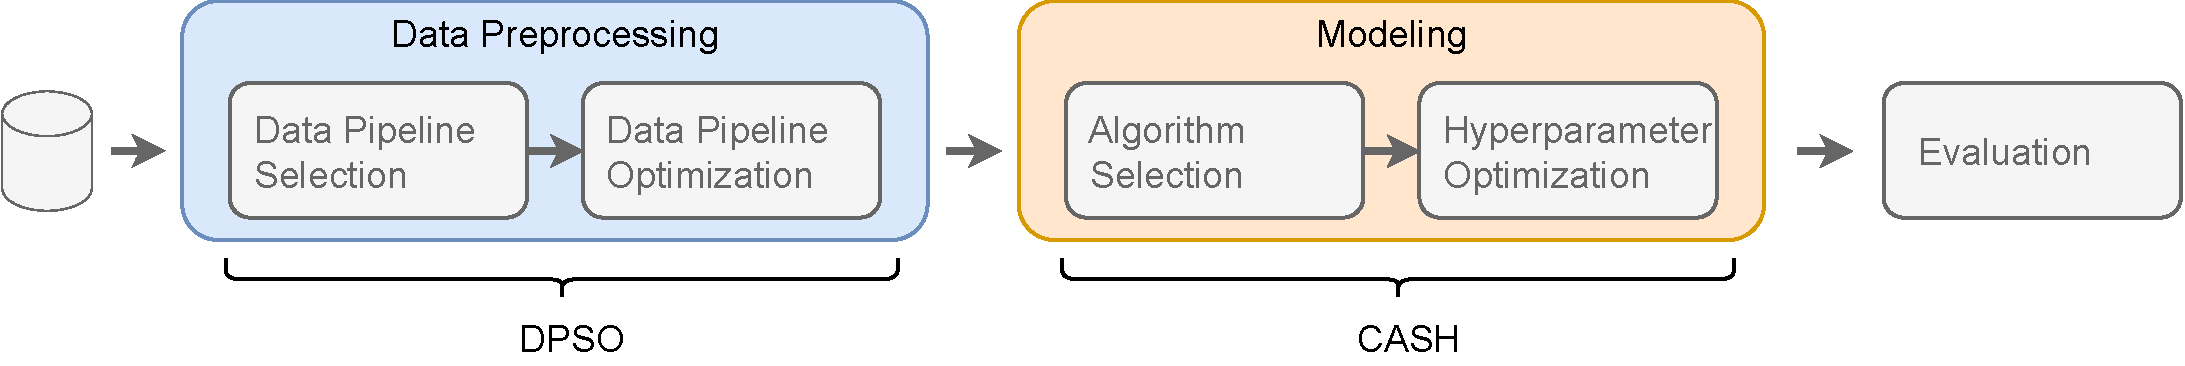
\includegraphics[width=1.0\textwidth]{chapters/data-centric/supervised/img/data-analytics-pipeline.pdf}
    \caption{Data analytics pipeline generation in a knowledge discovery process.}
    \label{effective-fig:data-analytics-pipeline}
\end{figure*}

To unleash the full potential of ML, data-centric AI focuses on shaping data according to the task and algorithm at hand.
With reference to the CRISP-DM process model,  \Cref{effective-fig:data-analytics-pipeline} summarizes the stages involved and the corresponding problems in the literature.
Firstly, data are extracted in a raw format from different sources and sifted out so that only a relevant subset is selected.
Next, during the pre-processing stage, the data pipeline selection and optimization (DPSO) \cite{Quemy19DOLAP} problem is tackled.
Once the data is transformed into the proper form, the modelling stage focuses on the combined algorithm selection and hyperparameter (CASH) optimization problem.
Finally, pipelines and algorithms
are evaluated over the dataset until an acceptable result is obtained.

It is well-known that the whole process requires expertise and is particularly challenging.
Particularly, data scientists spend most of their time on the heavily laborious work of pre-processing (i.e., around 50-80\% of the total \cite{Munson09Pre}).
Some AutoML frameworks \cite{auto_sklearn, mohr2018ml}, mix-in pre-processing during modelling optimization, but typically include very few transformations or do not consider all the necessary steps (e.g., imputation, rebalancing), thus in a way overlooking it.
Inspired from \cite{Munoz09DOLAP}, we contend that there is need for more data-centric techniques, encompassing all the steps of data pre-processing \cite{Vaisman14Book}.
Assistance is required in every phase \cite{Bilalli16IOTBD}.
By considering pre-processing as an integral component of the learning process, and carefully selecting and optimizing data pipelines, it is easy to obtain results that go beyond the ones obtained by only optimizing ML algorithms.

To briefly illustrate this, we perform an experiment on the well known \texttt{bank-marketing}\footnote{\url{https://archive.ics.uci.edu/ml/datasets/Bank+Marketing}} dataset, using HyperOpt \cite{HyperOptICML13} as an AutoML approach to optimize the parameters of three different ML algorithms, namely Naive Bayes (NB), K-Nearest Neighbor (KNN), and Random Forest (RF).
We provide an initial budget of 50 iterations for optimizing the hyperparameters of the algorithms, and after the 50th iteration, we fix the algorithm configuration to the best one achieved so far and start optimizing the pre-processing pipeline\footnote{This order is used only for the sake of illustration.}.
In \Cref{effective-fig:pre-processing-impact}, the ratio of the change in terms of accuracy (i.e., obtained after the i-th iteration to the baseline/default accuracy) is plotted against the number of different configurations visited by HyperOpt (i.e., iterations).
Observe that after the 11th iteration for NB and KNN, and after the 26th iteration for RF, the lines remain flat.
That is, from there on, no improvement is achieved by optimizing the hyperparameters of the algorithms until the 50th iteration is reached. At this point, a sudden jump is observed and the results start to improve again, going clearly beyond the ones obtained before, thanks to the optimizations performed now over the pre-processing pipeline.

\begin{figure}[t]
    \centering
    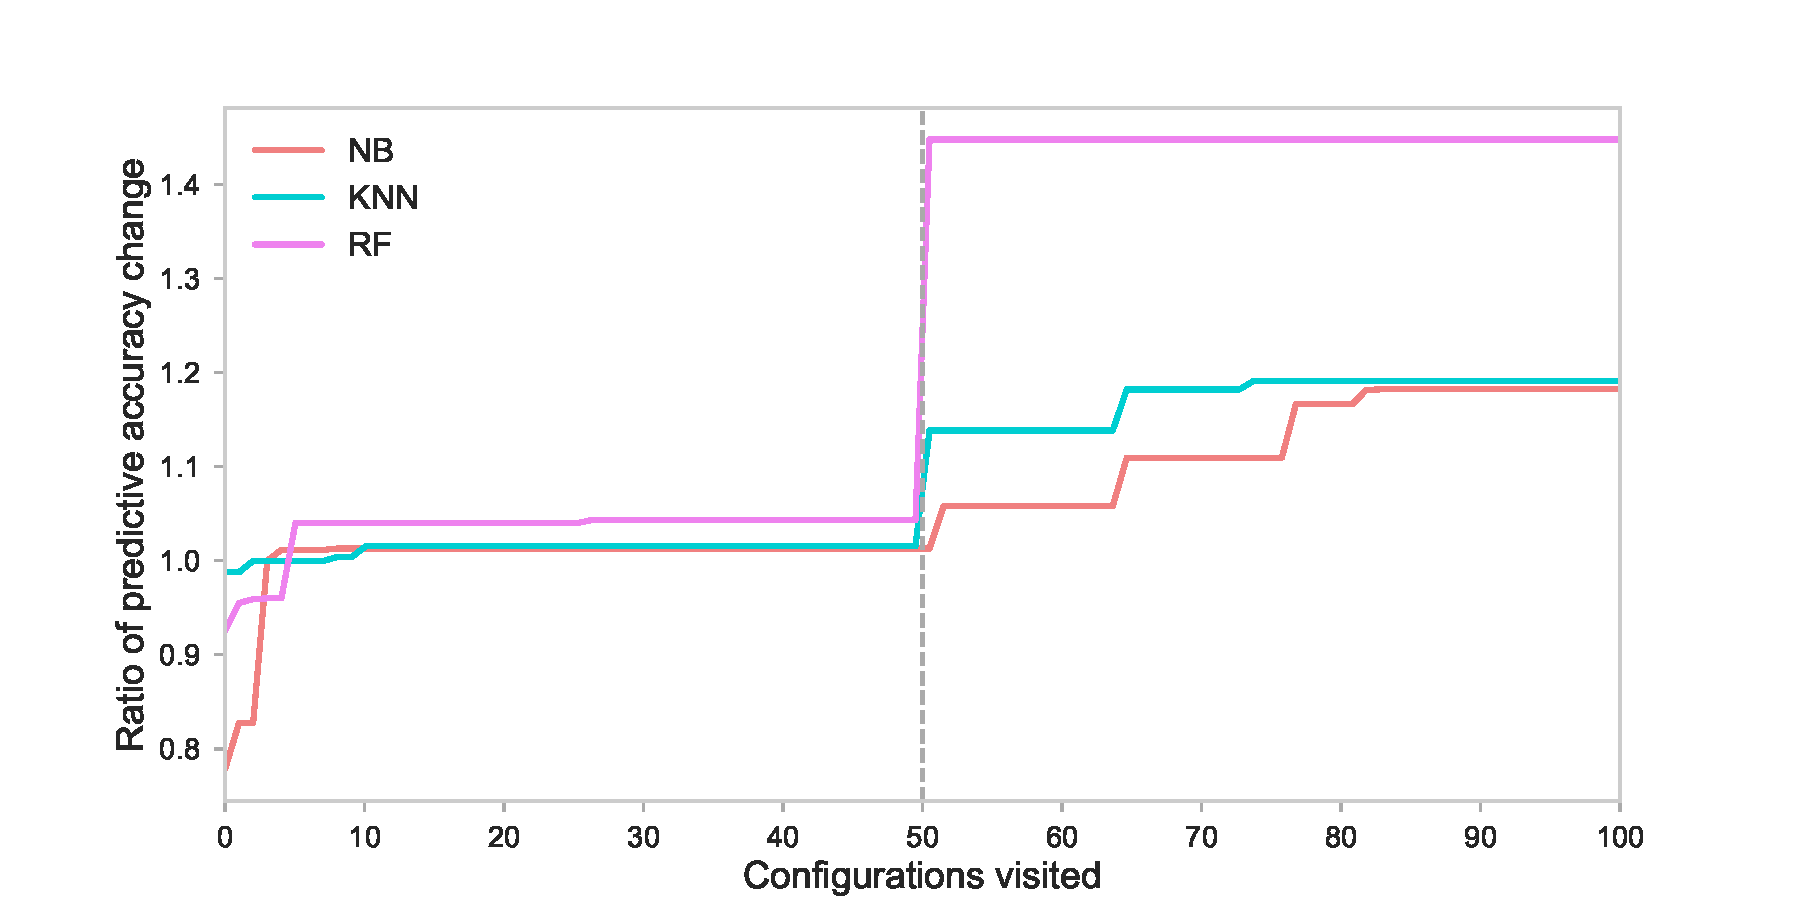
\includegraphics[width=0.7\textwidth]{chapters/data-centric/supervised/img/pre-processing-impact.pdf}
    \caption{Evolution of accuracy during the optimization process. The first 50 configurations optimize only the hyperparameters and after the 50th configuration, the pre-processing pipeline is optimized instead.}
    \label{effective-fig:pre-processing-impact}
\end{figure}

\paragraph{Challenges} Including pre-processing in the learning process heavily increases the search space, making the problem much harder.
DPSO entails two challenges that the data scientists have to undergo to find the most appropriate pipeline: (i) choose how to order the different pre-processing steps  (i.e., pipeline selection), and (ii) choose which transformations, with corresponding hyperparameters, should be adopted in the final implementation  (i.e., pipeline optimization).
To better distinguish between pipeline selection and its optimization, we follow the notation from \cite{Quemy20InfSystems}: a \textit{prototype} is the fixed and ordered sequence of pre-processing steps, its optimized instantiation of each transformation (with their hyperparameters) is known as \textit{executable pipeline}.

\paragraph{Contributions} The aim of this chapter is to study the two questions raised and propose a method for selecting effective pre-processing prototypes that, once optimized through some optimization technique (e.g., Bayesian optimization), improve the final result of the analysis.
To keep discussions and experiments simpler, we stick to supervised learning tasks.
The main contributions can be summarized as follows.
\begin{itemize}
    \item We empirically evaluate the impact of optimizing the exhaustive set of potential prototypes and find out that	there is no universal solution---i.e., prototype that works best for each dataset and algorithm considered.
    \item We define a method that given an ML algorithm and a set of pre-processing steps, is capable of generating the right order, obtaining effective pre-processing prototypes that are then instantiated via bayesian optimization.
    \item We suggest a meta-learning step (i.e., learning on top of learning) where the relationships between pre-processing transformations and dataset characteristics are learned in order to create rules that help with the initial instantiation of the prototypes.

	We exemplify our meta-learning study generating simple but not obvious and effective rules for two kinds of pre-processing steps, namely, Feature Engineering and Rebalancing.
    \item We perform a comprehensive evaluation by comparing the performance of optimizing prototypes generated following our method, and find out that:
    \begin{enumerate}
        \item with 24 times less time budget, our proposed pipelines obtain results whose median is above 90\% of the ones generated via exhaustive search.
        \item on average, in 73\% of the cases, splitting evenly the time budget between pre-processing and modelling outperforms the results of solely optimizing the latter.
    \end{enumerate}
	\item We deploy \textbf{AutoPrep}, a reproducibility framework for the automatic generation of effective pre-processing pipeline prototypes. Specifically, in \cite{giovanelli2023reproducible}, we introduce: (i) a detailed reproducibility protocol, (ii) software, and (iii) datasets in a self-contained environment.
	The experiments were run on several machines and confirmed all the inishts in this chapter.
\end{itemize}

The remaining of this chapter is organized as follows:
\Cref{effective-sec:related-work} discusses the related work,
\Cref{effective-sec:methodology} presents our method of generating effective pipelines,
\Cref{effective-sec:evaluation} provides an extensive evaluation of the pipelines created using our proposed method and, finally, \Cref{effective-sec:conclusions} provides the conclusions and future work.


\section{Related Works}
\label{effective-sec:related-work}
At the beginning, the AutoML community followed the AI trend of contributing under a more algorithmic perspective, focusing on modelling---i.e., the resolution of the CASH problem.
Recently however, the direction has shifted towards designing systems that additionally or specifically provide user assistance in the data pre-processing step---i.e., solving the DPSO problem.
We can categorize works according to the optimization policy \cite{quemy2019data} they adopt.
On the one hand, some automate data pre-processing via split-like policies---i.e., addressing DPSO in isolation from CASH (\Cref{effective-ssec:dpso}).
On the other hand, some consider optimizing DPSO along with CASH, adopting a joint policy---data pre-processing in synergy with modelling (\Cref{effective-ssec:dpso-cash}).

\subsection{Optimization with Split-like Policies}
\label{effective-ssec:dpso}

In \cite{Quemy20InfSystems}, authors demonstrate the impact of optimizing the pre-processing pipelines, but considering only a single fixed prototype and only a few datasets.
However, as we have already seen (\Cref{effective-sec:eval-universal-pipeline}), a single fixed prototype cannot perform best for every dataset.

In PRESISTANT \cite{presistant18CSI,presistant18CAISE,presistant19DKE}, authors tackled the problem of recommending pre-processing transformations to non-expert users.
They identify the pre-processing transformations and rank them in advance, based on their potential impact to the final analysis.
However, they do not consider pre-processing pipelines, but only single transformations, expecting that the analyst applies the process iteratively.

In ActiveClean \cite{ActiveClean16PVLDB}, authors define a method that aims at prioritizing the cleaning of records that are more likely to affect the results of the analysis, assuming that the latter belongs to the class of convex loss models (i.e., linear regression and SVMs).
Hence, instead of recommending the transformations to be applied, the system recommends the subset of data that needs to be cleaned at a given point.
The type of pre-processing to be applied is left to the user, assuming that the user is an expert.

In Learn2Clean \cite{Berti19WWW}, based on a reinforcement learning technique, for a given dataset and an ML model, an optimal sequence of pre-processing transformations is generated so that the quality of the ML model is maximized.
Yet, similarly to \cite{Quemy20InfSystems}, the pipeline prototype is fixed in advance.

In Alpine Meadow \cite{Shang19SIGMOD}, authors follow a similar approach to ours in that they define two steps for the pre-processing phase. One, the so-called \textit{logical pipeline plan}, which is roughly equivalent to the \textit{prototype} defined in this work, and the second the \textit{physical pipeline plan} which translates to \textit{executable pipelines} used in this work.
The physical plan is generated through a combination of Bayesian optimization, meta-learning, and multi-armed bandits.
For the logical plans, they rely on rules but without clear evidence on how they are generated.
Moreover, it is not clear whether the logical plan is fixed as in \cite{Quemy20InfSystems} and if some further adjustment from the user is required.

\subsection{Optimization with a Joint Policy}
\label{effective-ssec:dpso-cash}
Auto-sklearn \cite{Feurer15AutoSklearn} is based on the popular Python library scikit-learn.
The authors, inspired by Auto-Weka, address the problem with the Sequential Model-based Algorithm Configuration (SMAC).
Furthermore, they improve the approach by adding a meta-learning phase (i.e., learning on top of learning) at the beginning and an ensemble technique at the end.
Meta-learning leverages previous ML experiments and learns promising configurations to warm-start (i.e., boost the convergence) the Bayesian Optimization.
Ensemble techniques merge predictions from multiple ML models to statistically outperform the base models.
Yet, they consider a small set of transformations and also consider a single fixed prototype.

TPOT \cite{Olson16Tpot} is a tree-based pipeline optimization tool using genetic programming while requiring little to no expertise from the user.
In TPOT however, they only consider one transformation inside the optimization process (i.e., Feature Engineering).

ML-Plan \cite{mohr2018ml} uses hierarchical planning, a particular form of AI planning, to propose a solution to both the pre-processing and the modeling phases.
As in context-free grammars, there are complex tasks (non-terminal symbols) that are derived as long as primitive tasks (terminal symbols) are not obtained.
Typically, standard graph search algorithms (e.g., depth-first search, best-first search, etc.) are employed to solve such problems.
ML-Plan successively creates solutions in a global search instead of changing given solutions in a local search. However, due to the problem constraints, they adopt a randomized best-first search, randomly choosing the solution path.

AutoBazaar \cite{AutoBazaar} is a Python open-source tool.
Like in ML-Plan \cite{mohr2018ml}, both pre-processing and modeling phases are covered.
Here the last step of a prototype is the machine learning algorithm.
The approach involves two different steps.
Firstly, a \textit{catalog} proposes a collection of prototypes (with an ML algorithm as last step) based on the task and the dataset itself.
Secondly, the optimization process starts tuning the prototypes until either the time budget is expired or the prototypes are all optimized.
In particular, a \textit{selector} and a \textit{tuner} work in synergy.
The former decides which prototype should be optimized next.
Such a task is treated as a multi-armed bandit problem.
As to the tuner, bayesian optimization is chosen.
At the end, the prototype that achieved the higher accuracy is elected.
However, AutoBazaar strictly depends on the catalog.
Such a component memorizes all the possible primitives and supported tasks.
The prototypes are hard-coded for each task.
Thus, it is neither flexible nor maintainable.
If a task is not implemented, the approach cannot suggest a solution.

To summarize, full automation of data analytics has been the ultimate goal of many research works.
Yet, such automation has shown to be computationally expensive, mainly due to the search space involved (i.e., pre-processing and mining operators).
Therefore, the usability of these approaches in realistic scenarios is sometimes limited.
Our approach of finding a set of effective prototypes can be seen as complementary to these solutions, since it helps in pruning the large space and guiding the search, hence reducing their cost.

\section{Effective Data Pre-processing Pipeline Generation}
\label{effective-sec:methodology}

We aim to find the best data pipeline (i.e., with higher performance) for the dataset $\altmathcal{D}$ and the ML algorithm $A$ considered, hence solving DPSO.
Let us refresh the formalization of interest.

Each transformation $T$ exposes a set of $K$ hyperparameters, producing the Cartesian product $\Lambda_T = \Lambda_1 \times \dots \times \Lambda_K$.
A pre-processing \textit{step} $S$ can be instantiated from several alternative transformations, hence $\Lambda_S = \Lambda_{T_1} \cup \ldots \cup \Lambda_{T_{|S|}} \cup \lambda_s$, with $\lambda_s$ a new root-hyperparameter that selects the transformation.
The problem exacerbates when steps are combined together into data pipelines.
Indeed, the complete search space for our optimization problem is defined as $\Lambda_P = \Lambda_{S_1} \times \ldots \times \Lambda_{S_{|P|}} \times \lambda_p$, with $\lambda_p$ as yet another root-hyperparameter to select -- this time -- the order between the transformations (translating into the disjoint union of all partial permutations).

To mitigate the problem's complexity, we distinguish between pipeline selection and its optimization.
Specifically, following the notation from \cite{quemy2019data}:
pipeline selection aims at finding promising \textit{prototypes}, i.e. fixed and ordered sequence of pre-processing steps, pipeline optimization instantiates the best \textit{executable pipeline}, i.e. assigning a transformation (along with the hyperparameters) to each pre-processing step.

\begin{figure*}[t]
    \centering
    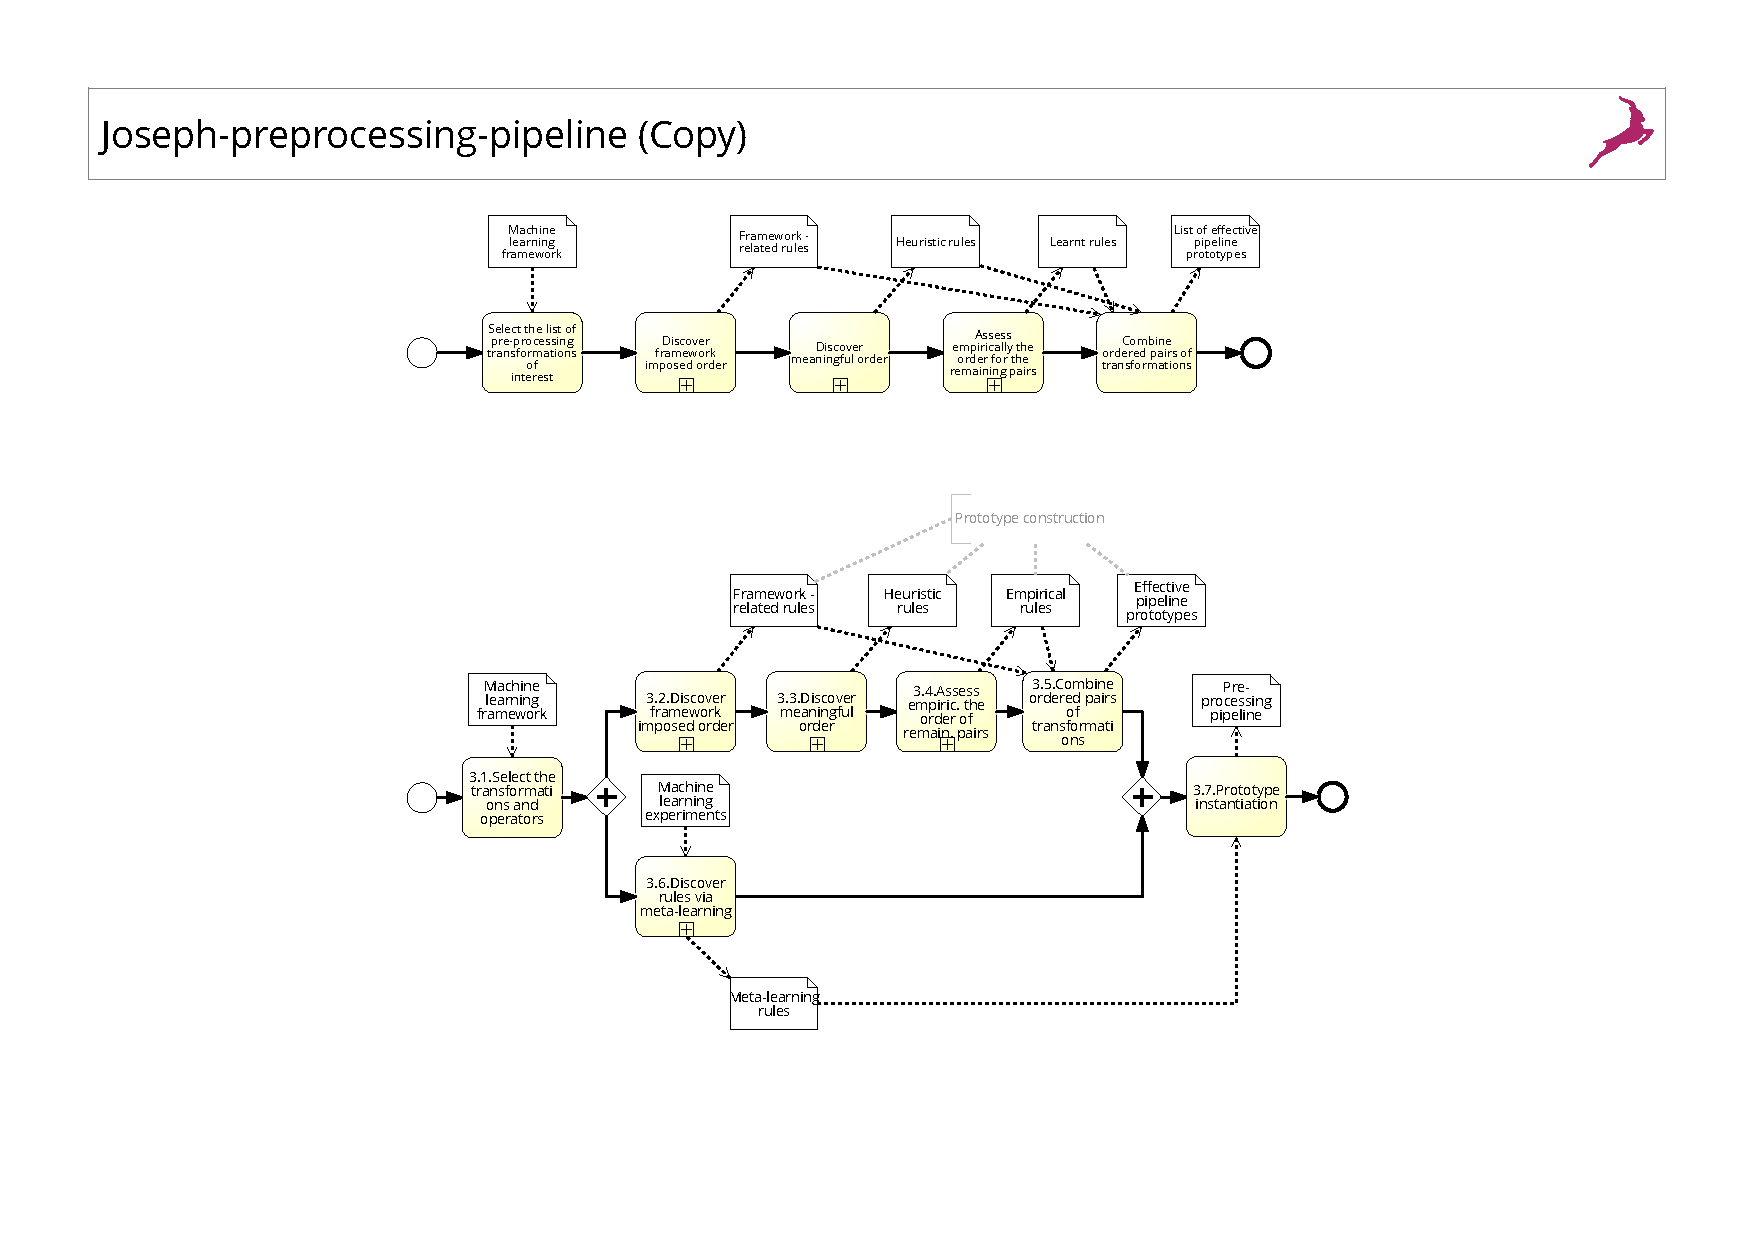
\includegraphics[width=1.0\textwidth]{chapters/data-centric/supervised/img/bpmn.pdf}
    \caption{A method for generating effective pre-processing pipelines}
    \label{effective-fig:methodology}
\end{figure*}

\Cref{effective-fig:methodology} sketches the proposed methodology, some of the phases are generic and thus can be applied regardless of the context, and yet others are specific (i.e., ML framework or dataset characteristics).
According to \cite{Quemy20InfSystems}, we break the combinatorial problem into two workflows: (i) studying pre-processing steps in pairs for generating effective prototypes and then (ii) feeding them to an optimizer (e.g., we use the SMBO \cite{HyperOptICML13} variant) for their actual instantiation.

\paragraph{Effective Prototypes Generation} The proposed method starts with the selection of the ML library (\Cref{effective-ssec:select-framework}).
This allows to consider solely the steps for which their implementation is available.
Besides, with such a choice, we are also provided with a set of \textit{framework-related rules} (\Cref{effective-ssec:rules-framework}), constraining the possible orderings of the steps (e.g., in scikit-learn, Imputation has to be the first step in the prototype).
These rules are in the form of precedences of pre-processing steps (i.e. orderings that involve two steps at a time;  e.g., Imputation before Normalization).
Next, the flow on top continues with a study
aiming to find the correct/meaningful orderings according to
the behavior of the transformations in each step.
As a result, this generates a set of \textit{heuristic rules} (\Cref{effective-ssec:rules-heuristics}) that restrict the space of possible precedences.
Afterward, for the pairs for which an order cannot be clearly devised, an additional empirical study is proposed.
This study relies on a test bed of representative datasets.
The output is a set of \textit{empirically-learned rules} (\Cref{effective-ssec:rules-learned}) that determines yet other precedences, namely promising orderings that would potentially positively impact the final result of the analysis.
However, even after this phase, for some pairs of pre-processing steps, a precedence order may not be found.
These are pairs for whom the order is relevant but cannot be decided in advance, thus all their permutations need to be present.
Finally, a step of composition follows  (\Cref{effective-ssec:composition}), where given the overall set of devised rules (i.e., \textit{framework-related}, \textit{heuristic} and \textit{empirically-learned}), the pre-processing steps are composed into a set of valid and potentially effective prototypes.

More formally, when combining two different pre-processing steps, it is important to check if, (i) the input and output types of the steps are compatible, (ii) the combination makes sense, and (iii) the combination provides good results for the analysis.
As a result, when chaining a pair of steps, the following precedence relationships arise:
\begin{enumerate}
    \item Compatible/Incompatible. Depending on whether the representation output of the first step is accepted as the representation input of the second one (compatible), or not (incompatible).
    \item Meaningful/Meaningless. Depending on whether the precedence between them makes sense based on generic knowledge (i.e., based on the literature) over the behaviour of transformations (meaningful), or not (meaningless).
    \item Promising/Unpromising. Depending on whether the precedence between them is expected to provide a positive impact on the final result of the analysis (promising), or not (unpromising).
\end{enumerate}

Attending to the relationships between its steps, a prototype can be described as either \textit{compatible}, \textit{well-formed}, or \textit{effective}.
A prototype is defined to be \textit{compatible} if all its precedence relationships are available in the ML framework at hand.
It is defined as \textit{well-formed} if all its precedence relationships are both compatible and meaningful.
Finally, it is defined as \textit{effective} if all its precedence relationships are compatible, meaningful, and promising at the same time.
In fact, the goal of this flow is to find \textit{effective prototypes}.

\paragraph{Warm-starting via Meta-learning} Once the prototype is constructed, the flow running in parallel is proposed to help with its instantiation.
It consists of a meta-learning step  (\Cref{effective-ssec:meta-learning}), where a set of ML experiments (e.g., pre-processing and classification algorithm runs) are used as training data to predict promising transformations for a pre-processing step.
These rules extract knowledge from past experiments and are complementary to the rules obtained in the first flow.
This practice is called warm-starting,
They would be used, for example, to ease the cold start problem in the prototype instantiation phase  (\Cref{effective-ssec:prototype-insta}).

We propose a generic methodology.
However, to keep the reader from losing, we will illustrate our use case and corresponding findings along with the explanation of the methodology.

\subsection{Selection of Data Pre-Processing Steps and Transformations}
\label{effective-ssec:select-framework}

The first task in the process consists of selecting the data pre-processing steps and their available transformations according to the selected ML library.

\paragraph{Use case}
For our experiments, we selected the pre-processing steps, transformations and hyperparameters from those available in the scikit-learn library\footnote{\url{https://scikit-learn.org}} (\Cref{effective-tbl:transformations}).
\textit{Input} denotes the compatible feature type for a given pre-processing step and can be continuous (CO) -- when it represents measurements on some continuous scale -- or categorical (CA)---when it represents information about some categorical or discrete characteristics.
Similarly, \textit{Output} denotes the type of the features after a pre-processing step is applied.

\begin{itemize}[noitemsep,topsep=0pt]
\item{Encoding ($E$).} The process of transforming categorical features into continuous ones (here, we refer solely to the encoded representation, not the semantic).
\item{Normalization ($N$).} The process of normalizing continuous features such that their values fall in the same range.
\item{Discretization ($D$).} The process of transforming continuous features into categorical ones.
\item{Imputation ($I$).} The process of imputing missing values.
\item{Rebalancing ($R$).} The process of adjusting the class distribution of a dataset (i.e. the ratio between the different classes/categories represented).
\item{Feature Engineering ($F$).} The process of defining the set of relevant features to be used in model training.
\end{itemize}

Finally, \textit{transformations} denotes the actual instantiation for the step, and it can be tuned using its \textit{hyperparameters}.


\begin{table}[!t]
\renewcommand{\arraystretch}{0.3}
\footnotesize
\caption{List of transformations applicable to categorical or continuous data types.}
\centering
\begin{threeparttable}

\begin{tabular}{@{}p{30mm}lll>{\ttfamily}l@{}}
\toprule
Pre-processing Step& Input & Output & Transformation & \textnormal{Hyperparameters}
\\	\cmidrule[.1em]{1-5}

Encoding ($E$)  & CA & CO & Ordinal & -  \\ \cmidrule[.05em]{4-5} & & & One Hot & - \\
\cmidrule[.1em]{1-5}

Normalization ($N$) & CO & CO & Standard Scaler & with\_mean:[True,False]\\ \cmidrule[.05em]{4-5} & & & & with\_std:[True,False] \\ \cmidrule[.05em]{4-5}
&  &  & Power Transform & -\\ \cmidrule[.05em]{4-5}
&  &  & MinMax Scaler & -\\ \cmidrule[.05em]{4-5}
&  &  & Robust Scaler & quantile\_range:[(25,75),(10,90),(5,95)]\\ \cmidrule[.05em]{4-5} & & & & with\_centering:[True,False]\\ \cmidrule[.05em]{4-5} & & & & with\_scaling:[True,False] \\
\cmidrule[.1em]{1-5}

Discretization ($D$) & CO & CA & KBins & n\_bins:[3,5,7]\\ \cmidrule[.05em]{4-5} & & & & encode:[`onehot',`onehot-dense',`ord.']\\ \cmidrule[.05em]{4-5} & & & & strategy:[`uniform',`quant.',`kmeans']\\	\cmidrule[.05em]{4-5}
&  &  & Binarization  & threshold: [0, 0.5, 2, 5]\\	\cmidrule[.1em]{1-5}

Imputation ($I$) & CA/CO & CA/CO  & Univariate & strategy:[`most\_freq.','constant'] \\	\cmidrule[.05em]{4-5}
 & &  & Multivariate & initial\_strategy:[`most\_freq',`const.']\\ \cmidrule[.05em]{4-5} & & & & order:[`asc',`dsc',`rom',`arab',`rand'] \\	\cmidrule[.1em]{1-5}

Rebalancing ($R$)* &CA/CO  & CA/CO & Near Miss & n\_neighbors:[1,2,3]\\ \cmidrule[.05em]{4-5}
%&  &  & \textcolor{red}{Condensed KNN} & \textcolor{red}{n\_neighbors:[1,2,3]} \\ \cmidrule[.05em]{4-5}
&  &  & SMOTE & k\_neighbors:[5,6,7]\\	\cmidrule[.1em]{1-5}

Feat. Eng. ($F$) & CA/CO & CA/CO & PCA & n\_components:[1,2,3,4]\\ \cmidrule[.05em]{4-5}
&  &  & Select K Best & k:[1,2,3,4]\\ \cmidrule[.05em]{4-5}
&  &  & PCA + Select K Best  & n\_components:[1,2,3,4]
\\ \cmidrule[.05em]{4-5} & & & & k:[1,2,3,4]\\	\bottomrule%\cmidrule[.1em]{1-5}
\end{tabular}
\begin{tablenotes}
\footnotesize
\item CA - categorical, CO - continuous.
\item *All transformations except Rebalancing are taken from scikit-learn.
\end{tablenotes}
\end{threeparttable}
\label{effective-tbl:transformations}
\end{table}

\begin{table*}[!t]
    \caption{
        Precedence order between pairs of pre-processing steps, represented independently for each phase.
        }
    \renewcommand{\arraystretch}{0.3}
    \footnotesize
    \begin{center}
    \subfloat[Compatible precedence.]{
    \begin{tabular}{@{}lcccccc}
    \toprule
     & $\boldsymbol{E}$ & $\boldsymbol{N}$ & $\boldsymbol{D}$ & $\boldsymbol{I}$ & $\boldsymbol{R}$ & $\boldsymbol{F}$
    \\	\cmidrule[.1em]{1-7}
    $\boldsymbol{E}$ & \cellcolor{gray!25} & \texttt{1} & \texttt{1} & \texttt{\texttt{0}} & \texttt{1} & \texttt{1} \\	\cmidrule[.1em]{1-7}
    $\boldsymbol{N}$ & \texttt{0} & \cellcolor{gray!25}  & \texttt{0} & \texttt{0} & \texttt{0} & \texttt{0} \\	\cmidrule[.1em]{1-7}
    $\boldsymbol{D}$ & \texttt{0} & \texttt{0} & \cellcolor{gray!25}  & \texttt{0} & \texttt{0} & \texttt{0} \\	\cmidrule[.1em]{1-7}
    $\boldsymbol{I}$ & \texttt{1} & \texttt{0} & \texttt{1} & \cellcolor{gray!25}  & \texttt{1} & \texttt{1} \\	\cmidrule[.1em]{1-7}
    $\boldsymbol{R}$ & \texttt{0} & \texttt{0} & \texttt{0} & \texttt{0} & \cellcolor{gray!25}  & \texttt{0} \\	\cmidrule[.1em]{1-7}
    $\boldsymbol{F}$ & \texttt{0} & \texttt{0} & \texttt{0} & \texttt{0} & \texttt{0} & \cellcolor{gray!25}
    \\	\bottomrule
    \end{tabular}}
    \qquad% --- set horizontal distance between tables here
    \subfloat[Meaningful precedence.]{%
    \begin{tabular}{@{}lcccccc}
    \toprule
    & $\boldsymbol{E}$ & $\boldsymbol{N}$ & $\boldsymbol{D}$ & $\boldsymbol{I}$ & $\boldsymbol{R}$ & $\boldsymbol{F}$
    \\	\cmidrule[.1em]{1-7}
    $\boldsymbol{E}$ & \cellcolor{gray!25} & \texttt{0} & \texttt{0} & \texttt{0} & \texttt{0} & \texttt{0} \\	\cmidrule[.1em]{1-7}
    $\boldsymbol{N}$ & \texttt{0} & \cellcolor{gray!25}  & \texttt{X} & \texttt{0} & \texttt{1} & \texttt{0} \\	\cmidrule[.1em]{1-7}
    $\boldsymbol{D}$ & \texttt{0} & \texttt{X} & \cellcolor{gray!25}  & \texttt{0} & \texttt{0} & \texttt{0} \\	\cmidrule[.1em]{1-7}
    $\boldsymbol{I}$ & \texttt{1} & \texttt{1} & \texttt{1} & \cellcolor{gray!25}  & \texttt{1} & \texttt{1} \\	\cmidrule[.1em]{1-7}
    $\boldsymbol{R}$ & \texttt{0} & \texttt{0} & \texttt{0} & \texttt{0} & \cellcolor{gray!25}  & \texttt{0} \\	\cmidrule[.1em]{1-7}
    $\boldsymbol{F}$ & \texttt{0} & \texttt{0} & \texttt{0} & \texttt{0} & \texttt{0} & \cellcolor{gray!25}
    \\	\bottomrule
    \end{tabular}}
    \qquad% --- set horizontal distance between tables here
    \subfloat[Promising precedence.]{%
    \begin{tabular}{@{}lcccccc}
    \toprule
    & $\boldsymbol{E}$ & $\boldsymbol{N}$ & $\boldsymbol{D}$ & $\boldsymbol{I}$ & $\boldsymbol{R}$ & $\boldsymbol{F}$
    \\	\cmidrule[.1em]{1-7}
    $\boldsymbol{E}$ & \cellcolor{gray!25} & \texttt{0} & \texttt{0} & \texttt{0} & \texttt{0} & \texttt{0} \\	\cmidrule[.1em]{1-7}
    $\boldsymbol{N}$ & \texttt{0} & \cellcolor{gray!25} & \texttt{0} & \texttt{0} & \texttt{0} & \texttt{1} \\	\cmidrule[.1em]{1-7}
    $\boldsymbol{D}$ & \texttt{0} & \texttt{0} & \cellcolor{gray!25} & \texttt{0} & \texttt{0} & \texttt{1} \\	\cmidrule[.1em]{1-7}
    $\boldsymbol{I}$ & \texttt{0} & \texttt{0} & \texttt{0} & \cellcolor{gray!25} & \texttt{0} & \texttt{0} \\	\cmidrule[.1em]{1-7}
    $\boldsymbol{R}$ & \texttt{0} & \texttt{0} & \texttt{0} & \texttt{0} & \cellcolor{gray!25} & \texttt{0} \\	\cmidrule[.1em]{1-7}
    $\boldsymbol{F}$ & \texttt{0} & \texttt{0} & \texttt{0} & \texttt{0} & \texttt{0} & \cellcolor{gray!25}
    \\	\bottomrule
    \end{tabular}}
    \end{center}
    \begin{tablenotes}
    \centering
    \scriptsize
    \item$\boldsymbol{E}$ - Encoding; $\boldsymbol{N}$ - Normalization; $\boldsymbol{D}$ - Discretization; $\boldsymbol{I}$ - Imputation; $\boldsymbol{R}$ - Rebalancing; $\boldsymbol{F}$ - Feature Engineering. \item \texttt{1} - a precedence edge exists between the row and the column, \texttt{0} - a precedence edge does not exist between the row
    \item and the column, \texttt{X} - the combination is meaningless.
    \end{tablenotes}
    \label{effective-tbl:rules}
    \end{table*}

\subsection{Extraction of Compatible Precedences}
\label{effective-ssec:rules-framework}

Once the implementation framework is selected, one needs to study it and see if there exist constraints that limit the interaction between the pre-processing steps.
For instance, applying a step may actually invalidate the application of another one, because the compatibility of them is dependent on the selected ML framework.
We aim at detecting a set of implicit rules that are shown through an adjacency matrix, corresponding to a precedence graph as those in \Cref{effective-tbl:rules}.
Each cell $a_{ij}$ denotes a precedence relationship between the row $i$ and column $j$.
Hence, \texttt{1} means that an edge exists between the transformation in the row and the transformation in the column, whereas \texttt{0} means that such an edge does not exist, hence a precedence order is not established for that pair.

\paragraph{Use case}
We studied the pre-processing steps implemented in Scikit-learn, the discovered rules are shown through the adjacency matrix in \Cref{effective-tbl:rules}a.
For example, most Scikit-learn steps cannot be applied in the presence of missing values.
This is why in every pair of them where Imputation is involved, except the one with Normalization\footnote{Normalization transformations are the only ones that Scikit-learn can apply on datasets with missing values.}, Imputation goes first.
Furthermore, Scikit-learn steos are applied only to all compatible features of a given dataset.
Generally, categorical features are physically represented as strings and continuous features as numbers.
However, a transformation that is meant to be applied, say to continuous features, cannot be applied over a dataset that contains both continuous and categorical features (i.e., a dataset containing both numbers and strings); Scikit-learn cannot deal with arrays of mixed types.
In that case, all the categorical features need to be encoded into numeric representations, even if they represent a categorical value.
That is, a value can be a number but represent a category.
This is what happens when Normalization and Discretization are meant to be applied to a dataset containing mixed types of features.
In order for them to be applied to datasets of mixed types, an Encoding transformation needs to be applied first.
A similar constraint is imposed when considering Rebalancing and Feature Engineering, since these steps do not accept inputs containing strings (i.e., representing a categorical type).
For the rest of the pairs, there are no constraints imposed by the framework, thus any ordering is permitted, reflected by a \texttt{0} in \Cref{effective-tbl:rules}a.
The graph obtained in this case exclusively corresponds to the limitations of Scikit-learn (as a matter of fact, if another framework were to be chosen, it may have looked differently).

\subsection{Discovery of Well-formed Precedences}
\label{effective-ssec:rules-heuristics}
Once we have derived precedences based on the constraints of the framework, we can study the precedence independently and find \textit{meaningful pairs}.
That is, for every given pair, we want to find the relative order based on generic domain-independent knowledge (i.e., literature) about pre-processing steps and their applicability.
To this end, some of the constraints imposed by the framework may be contradicted here, but this is resolved in the last step of the proposed method (\Cref{effective-ssec:composition}).
Briefly, in a combination where Imputation is involved, it is advised to apply Imputation first.
Next, Encoding makes sense to be combined in any order with the rest of the transformations, except Imputation.
Combining Discretization with Normalization does not make sense, due to the fact that after the Discretization step, continuous features are transformed into categorical ones, and hence Normalization cannot be applied.
Similarly, applying Normalization first, changes the scale of the values and hence impacts the Discretization step.
Finally, a meaningful precedence can be derived when combining Normalization with Rebalancing.
In this case, Normalization should be applied first, since otherwise Rebalancing would impact the scale of the values to be normalized.

\paragraph{Use case}
\Cref{effective-tbl:rules}b shows the heuristic rules obtained considering domain-independent knowledge about the steps \cite{BookExploratoryDM03Dasu}.
In comparison with the results from \Cref{effective-tbl:rules}a, observe that the constraints on the Imputation still hold: when combining it ith another step, Imputation should go first.
This time even when combining it with Normalization---note the difference with \Cref{effective-tbl:rules}a.
The constraints of Encoding are however not present in \Cref{effective-tbl:rules}a, hence not considering the framework, Discretization combined with Encoding is a meaningful combination---when a mixed type dataset is considered, but incompatible from the point of view of Scikit-learn.

\subsection{Empirical-learning of Promising Precedences}
\label{effective-ssec:rules-learned}

The two previously proposed phases (i.e., \textit{framework-related} and \textit{heuristic rules}), do not guarantee that each pair of steps will obtain a precedence order.
Therefore, for those cases left out, a third viewpoint should be considered.
That of learning a promising order by empirically studying the impact of the combinations on the final result of the analysis, using different supervised problems in the training.
For every selected pair of pre-processing steps, for a given ML algorithm, we propose to check which order of the pair improves most the performance (e.g., accuracy) of the algorithm over a set of datasets (preferably from different domains).
Like this, for each dataset, we can get a precedence order that gives better results (i.e., promising precedence) in terms of the loss.


\begin{algorithm*}[!h]
	\caption{Find a promising prototype for steps $S_1$ and $S_2$}
	\label{effective-alg:learned-rules}
	\begin{algorithmic}[1]
		\Require $\altmathcal{D}_{train}$, $\altmathcal{D}_{valid}$, $A$, $\altmathcal{L}$ $S_1$, $S_2$ \Comment{dataset split for train and validation, classification algorithm, loss function, two different pre-processing steps}
		% \Require \indent$S_1\rightarrow S_2$, $S_2 \rightarrow S_1$ \Comment{precedence orders of a pair of transformations}
		\State $\altmathcal{L}_{\varnothing} = \altmathcal{L}(A(\altmathcal{D}_{train}), \altmathcal{D}_{valid})$ \Comment{get baseline performance of algorithm $A$ on $\altmathcal{D}$}
		\State $P_1 = \langle S_1, S_2 \rangle, P_2 = \langle S_2, S_1 \rangle$ \Comment{define two prototypes}
		\State $P_{1_{\lambda}} = SMBO(\langle P_1, A \rangle(\altmathcal{D}_{train}), \altmathcal{D}_{valid})$ \Comment{optimize the 1st prototype and get the best pipe}
		\State $\altmathcal{L}_{P_1} = \altmathcal{L}(\langle P_{1_{\lambda}}, A \rangle(\altmathcal{D}_{train}), \altmathcal{D}_{valid})$ \Comment{get the corresponding loss}
		\State $P_{2_{\lambda}} = SMBO(\langle P_2, A \rangle(\altmathcal{D}_{train}), \altmathcal{D}_{valid})$
		\Comment{optimize the 2nd prototype and get the best pipe}
		\State $\altmathcal{L}_{P_2} = \altmathcal{L}(\langle P_{2_{\lambda}}, A \rangle(\altmathcal{D}_{train}), \altmathcal{D}_{valid})$ \Comment{get the corresponding loss}
		% \State $[pipeline_{S_2\rightarrow S_1},acc_{S_2\rightarrow S_1}] = SMBO(S_2\rightarrow S_1,d, a)$
		% \Comment{get pipeline and accuracy for $S_2\rightarrow S_1$}
		% \If{\textit{IsValid}($acc_{S_1\rightarrow S_2},acc_{S_2\rightarrow S_1},acc_{baseline}$)}
		\If{$P_{1_{\lambda}}, P_{2_{\lambda}}$ are valid w.r.t. $\altmathcal{L}_{\varnothing}, \altmathcal{L}_{P_1}, \altmathcal{L}_{P_2}$}
        \Comment{see \Cref{effective-tbl:validation-rules} for the rules applied}
        \State \Return Best of $P_1$ and $P_2$
        \Comment{see column \textit{Winner prototype} in \Cref{effective-tbl:validation-rules}}
		\Else
		\State \Return $\varnothing$
		\EndIf
	\end{algorithmic}
\end{algorithm*}

\subsubsection{Experimental Learning Design}
To find a promising precedence order between a given pair of pre-processing steps $S_1$ and $S_2$, we propose \Cref{effective-alg:learned-rules}.
Let us consider a dataset split into $\altmathcal{D}_{train}$ and $\altmathcal{D}_{valid}$, a ML algorithm $A$, and a loss function $\altmathcal{L}$.
We first calculate $\altmathcal{L}_{\varnothing}$ as the loss of the ML algorithm $A$ over the original non-transformed dataset (line 1).
Afterward, to compute the impact of each possible prototype $P_1$ and $P_2$ (line 2), we leverage SMBO to find their optimized executable pipelines (line 3 and 5), and the losses of the ML algorithm (with default configuration) over the datasets transformed using the respective pipelines (line 4 and 6).
Based on the comparison between the respective optimized pipelines, we get the winner (line 7).
However, beforehand (line 6), we perform a validity check.
This is because when optimizing a pre-processing pipeline, SMBO may not instantiate a step with no transformation at all (i.e., represented with a $\varnothing$ symbol).
Hence, given a pair of pre-processing steps, where one or both of them may not be instantiated, SMBO may generate 16 possible scenarios.
They are listed in \Cref{effective-tbl:validation-rules}, and make up the validation rules for \Cref{effective-alg:learned-rules}.

\begin{table*}[t]
	\footnotesize
	\centering
	\begin{threeparttable}
	\caption{
		Validation rules.
		}
	\begin{tabular}{lp{2.3cm}p{2.3cm}p{2cm}p{2cm}p{2.5cm}}
	\toprule
	Nr. & Ex. Pipeline $P_{1_{\lambda}}$ & Ex. Pipeline $P_{2_{\lambda}}$ & Valid result & Valid score & Winner prototype\\\toprule
			1. &$\langle \varnothing, \varnothing \rangle$ & $\langle \varnothing, \varnothing \rangle$ & Draw          & $\altmathcal{L}_{\varnothing}$ &  Baseline \\ \hline
			2. &$\langle \varnothing, \varnothing \rangle$ & $\langle S_{2_{\lambda}}, \varnothing \rangle$ & Draw          & $\altmathcal{L}_{\varnothing}$ & Baseline \\ \hline
			3. &$\langle \varnothing, \varnothing \rangle$ & $\langle \varnothing, S_{1_{\lambda}} \rangle$ & Draw          & $\altmathcal{L}_{\varnothing}$ & Baseline \\ \hline
			\multirow{2}{*}{4.} &\multirow{2}{*}{$\langle \varnothing, \varnothing \rangle$} & \multirow{2}{*}{$\langle S_{2_{\lambda}}, S_{1_{\lambda}} \rangle$} & Draw & $\altmathcal{L}_{\varnothing}$ & Baseline \\
			& & & $P_{2_{\lambda}}$ & $\altmathcal{L}_{P_2}$ & $P_2$\\ \hline
			5. & $\langle \varnothing, S_{2_{\lambda}} \rangle$ & $\langle \varnothing, \varnothing \rangle$ & Draw          & $\altmathcal{L}_{\varnothing}$ & Baseline \\ \hline
			\multirow{3}{*}{6.} & \multirow{3}{*}{$\langle \varnothing, S_{2_{\lambda}} \rangle$} & \multirow{3}{*}{$\langle S_{2_{\lambda}}, \varnothing \rangle$} & Draw &  \multirow{3}{*}{$\altmathcal{L}_{S_2}$}  & $S_2$ \\
			& & & $P_{1_{\lambda}}$ & & $S_2$ \\
			& & & $P_{2_{\lambda}}$ & & $S_2$ \\ \hline
			7. &$\langle \varnothing, S_{2_{\lambda}} \rangle$ & $\langle \varnothing, S_{1_{\lambda}} \rangle$ & Draw & $\altmathcal{L}_{S_2}$ or $\altmathcal{L}_{S_1}$ & $S_{1}\,or\, S_2$ \\ \hline
			\multirow{2}{*}{8.} & \multirow{2}{*}{$\langle \varnothing, S_{2_{\lambda}} \rangle$} & \multirow{2}{*}{$\langle S_{2_{\lambda}}, S_{1_{\lambda}} \rangle$} & Draw & $\altmathcal{L}_{S_2}$ & $S_2$\\
			& & & $P_{2_{\lambda}}$ & $\altmathcal{L}_{P_2}$ & $P_2$ \\ \hline
			9. & $\langle S_{1_{\lambda}}, \varnothing \rangle$ & $\langle \varnothing, \varnothing \rangle$ & Draw & $\altmathcal{L}_{\varnothing}$ & Baseline \\ \hline
			10. & $\langle S_{1_{\lambda}}, \varnothing \rangle$ & $\langle S_{2_{\lambda}}, \varnothing \rangle$ & Draw & $\altmathcal{L}_{S_1}$ or $\altmathcal{L}_{S_2}$ & $S_{1}\,or\, S_2$ \\ \hline
			\multirow{3}{*}{11.} & \multirow{3}{*}{$\langle S_{1_{\lambda}}, \varnothing \rangle$} & \multirow{3}{*}{$\langle \varnothing, S_{2_{\lambda}} \rangle$} & Draw & \multirow{3}{*}{$\altmathcal{L}_{S_1}$} & $S_1$\\
			& & & $P_{1_{\lambda}}$ & & $S_1$\\
			& & & $P_{2_{\lambda}}$ & & $S_1$\\ \hline
			\multirow{2}{*}{12.} & \multirow{2}{*}{$\langle S_{1_{\lambda}}, \varnothing \rangle$} & \multirow{2}{*}{$\langle S_{2_{\lambda}}, S_{1_{\lambda}} \rangle$} & Draw & $\altmathcal{L}_{S_1}$  & $S_1$\\
			& & & $P_{2_{\lambda}}$ & $\altmathcal{L}_{P_2}$ & $P_2$ \\ \hline
			\multirow{2}{*}{13.} & \multirow{2}{*}{$\langle S_{1_{\lambda}}, S_{2_{\lambda}} \rangle$} & \multirow{2}{*}{$\langle \varnothing, \varnothing \rangle$} & Draw & $\altmathcal{L}_{\varnothing}$  & Baseline\\
			& & & $P_{1_{\lambda}}$ & $\altmathcal{L}_{P_1}$ & $P_1$ \\ \hline
			\multirow{2}{*}{14.} & \multirow{2}{*}{$\langle S_{1_{\lambda}}, S_{2_{\lambda}} \rangle$} & \multirow{2}{*}{$\langle S_{2_{\lambda}}, \varnothing \rangle$} & Draw & $\altmathcal{L}_{S_2}$ & $S_2$\\
			& & & $P_{1_{\lambda}}$ & $\altmathcal{L}_{P_1}$  & $P_1$ \\ \hline
			\multirow{2}{*}{15.} & \multirow{2}{*}{$\langle S_{1_{\lambda}}, S_{2_{\lambda}} \rangle$} & \multirow{2}{*}{$\langle \varnothing, S_{1_{\lambda}} \rangle$} & Draw & $\altmathcal{L}_{S_1}$ & $S_1$\\
			& & & $P_{1_{\lambda}}$ & $\altmathcal{L}_{P_1}$ & $P_1$\\ \hline
			\multirow{3}{*}{16.} & \multirow{3}{*}{$\langle S_{1_{\lambda}}, S_{2_{\lambda}} \rangle$} & \multirow{3}{*}{$\langle S_{2_{\lambda}}, S_{1_{\lambda}} \rangle$} & Draw & $\altmathcal{L}_{S_1}$ or $\altmathcal{L}_{S_2}$ & $S_{1}\,or\, S_2$ \\
			& & & $P_{1_{\lambda}}$ & $\altmathcal{L}_{P_1}$ & $P_1$\\
			& & & $P_{2_{\lambda}}$ & $\altmathcal{L}_{P_2}$ & $P_2$\\ \bottomrule
	\end{tabular}
	\begin{tablenotes}
	\footnotesize
	\item $\varnothing$ - SMBO finds a better result without instantiating a transformation for the step at hand.
	\item $S_{1_{\lambda}}, S_{2_{\lambda}}, P_{1_{\lambda}}, P_{1_{\lambda}}$ - A specific hyperparmeter configuration by SMBO for -- respectively -- $S_{1}, S_{2}, P_{1}, P_{2}$.
	\item $\altmathcal{L}_{S_1}, \altmathcal{L}_{S_2}, \altmathcal{L}_{P_1}, \altmathcal{L}_{P_2}$ - The loss of the ML algorithm over the data transformed when applied -- respectively -- solely $S_{1}$ or $S_{2}$, and the whole pipelines $P_{1}, P_{2}$.
	\end{tablenotes}
		\label{effective-tbl:validation-rules}
	\end{threeparttable}
\end{table*}

Briefly, if among the optimized pairs of steps (same steps but in reverse order) obtained from SMBO, one or both of them contain a $\varnothing$ transformation, their results are considered valid, only if they have equal scores (i.e., a draw).
This is because, if one has a higher score, it means that during the optimization it was more advantageous than the other, since it could find a configuration that should have been found by both of the pairs (given enough budget).
In our SMBO runs, such invalid results account for less than 10\% and in those cases datasets are discarded from the study.

In particular, in \Cref{effective-tbl:validation-rules}, the first two columns denote the executable pipelines for the respective prototypes (i.e., $\langle S_1, S_2 \rangle$ and $\langle S_2, S_1 \rangle$).
Next, \textit{valid result} denotes the expected result when comparing the results of the pipelines in the same row.
For instance, in the first row, if both steps in the pipelines are not instantiated during the optimization, a valid result is a draw, a \textit{valid score} is the baseline accuracy, and the \textit{winner prototype} is the prototype that is in accordance with the expected result, which in this case is the baseline (i.e., prototype where no transformations are applied).

For the sake of another example, let us check row 2 in \Cref{effective-tbl:validation-rules}.
Specifically, we consider the case in which, running SMBO, the best result for the first pair is the pipeline $\langle \varnothing, \varnothing \rangle$, and for the second pair is the pipeline $\langle S_2, \varnothing \rangle$.
Here, the comparison between the results of these pipelines should be equal (i.e., draw), and the score should be that of the baseline.
Otherwise, if say, the score of the second pipeline was higher, it would mean that for the first pair, SMBO was not given enough budget to find the pipeline with higher score (i.e., $\langle S_2, \varnothing \rangle$).
The same logic applies also to the other rows where a $\varnothing$ operator is involved.

\paragraph{Use case}
For the sake of this work, we considered three classification algorithms (i.e., \textit{NB}, \textit{RF},  \textit{KNN}) and $80$ datasets from the OpenML repository. The datasets, were compiled from three OpenML benchmarks, namely, the OpenMLCC18 benchmark\footnote{\url{https://www.openml.org/s/99/data}}, the AutoML benchmark\footnote{\url{https://www.openml.org/s/271/data}}, and the Classification algorithms benchmark\footnote{\url{https://www.openml.org/s/1/data}}.
For the final set, we filtered out datasets with more than 10\% of missing values -- not to include bias due to the heavy pre-processing we need to perform on top of them, and we filtered out the datasets with more than 5 million instances -- because of the computation time required to process them.
As a result, we obtained 60 datasets from the first benchmark, 17 from the second, and 3 more from the third to reach a total of 80 datasets.

Given the proposed algorithm (i.e., \Cref{effective-alg:learned-rules}), we could try to learn the precedence of every pair of steps, but would just be a waste of resources because we can see in Table~\ref{effective-tbl:rules}a and~\ref{effective-tbl:rules}b that some precedences are already decided for one reason or another.
Hence, only pairs with a \texttt{0} for both directions (in both Table~\ref{effective-tbl:rules}a and~\ref{effective-tbl:rules}b) need to be studied further.
That is, they make sense to be combined together, but a precedence order could not be determined through \textit{framework-related} or \textit{heuristic rules}. % for them.
Thus, for instance, pairs involving Encoding are not considered in this phase, since for them an order is already imposed by the framework (\Cref{effective-tbl:rules}a).
To this end, the pairs of transformations we consider for the third precedence graph include only $\{F,N\}$, $\{F,D\}$, $\{F,R\}$, and $\{R,D\}$.


\begin{figure*}[!b]
	\centering
	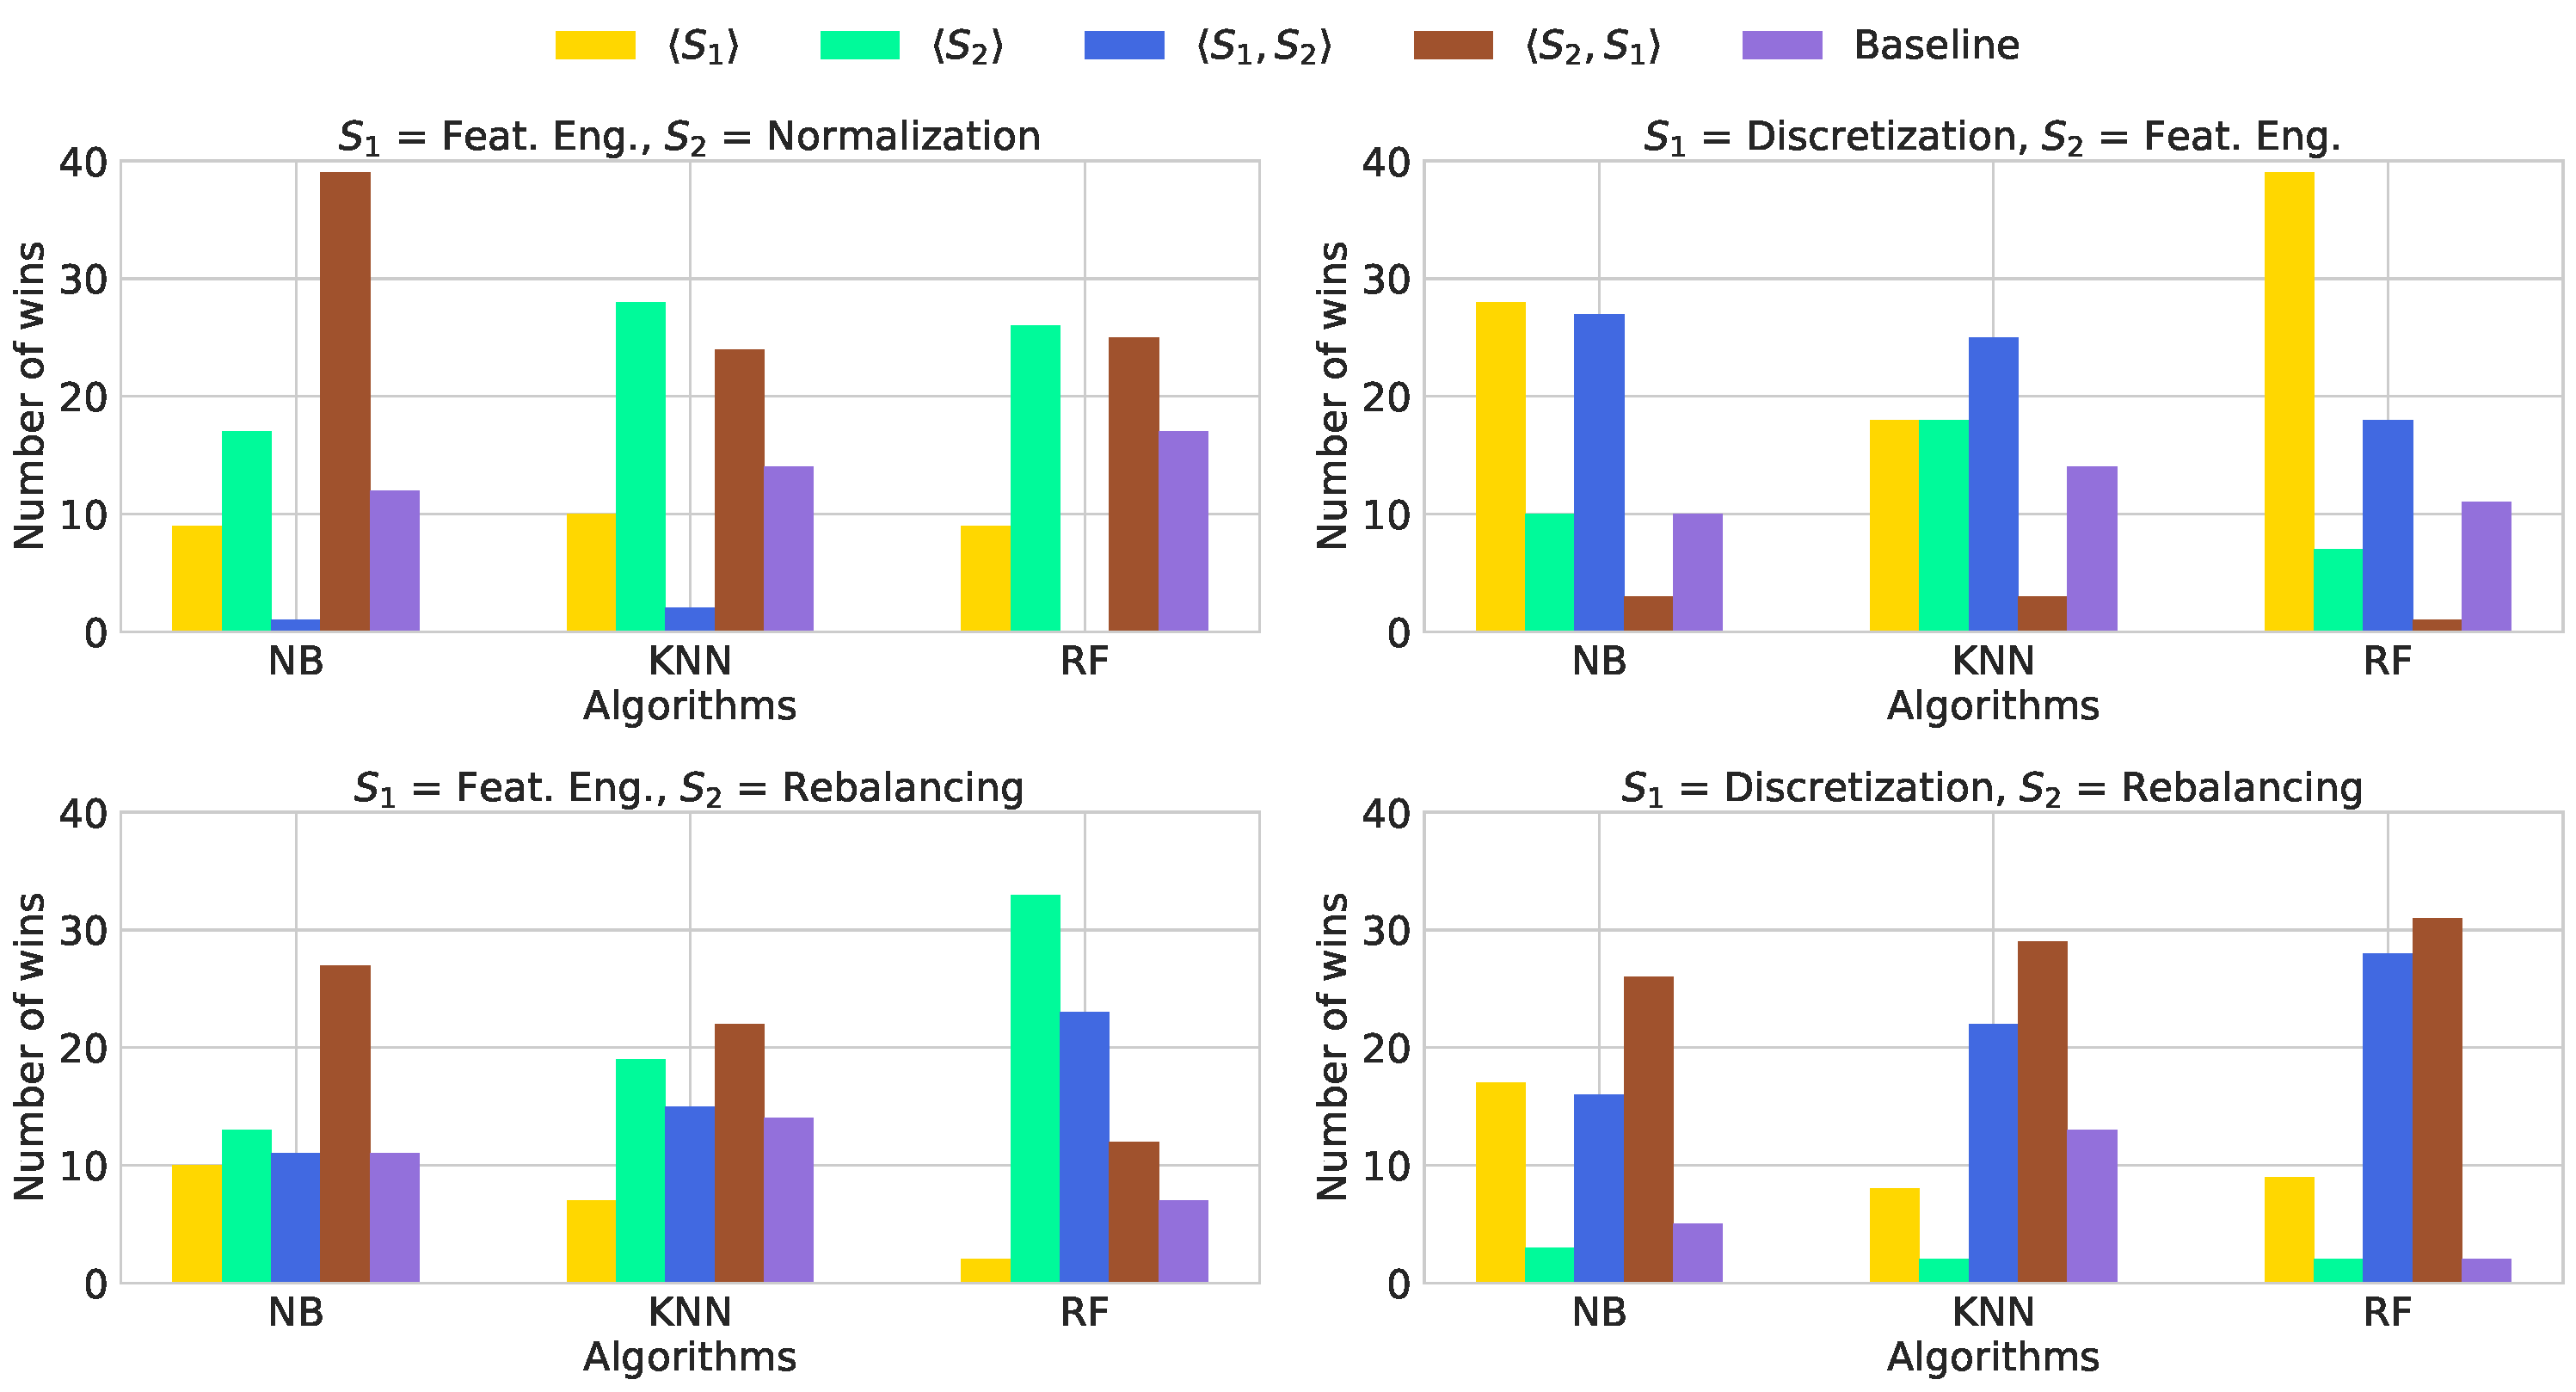
\includegraphics[width=1.0\textwidth]{chapters/data-centric/supervised/img/experiments_results.pdf}
	\caption{Number of datasets for which a given pipeline prototype is declared the winner.}
	\label{effective-fig:learned-rules-results}
\end{figure*}

Applying \Cref{effective-alg:learned-rules}, we obtain a promising order for each pair of transformations considered (i.e., $\{F,N\}$, $\{F,D\}$, $\{F,R\}$, $\{R,D\}$).
Since SMBO is a randomized algorithm, we experimented it with (i) running it several times splitting the budget, and (ii) running it only once with the entire budget.
For the experiments considered, no significant differences where observed, therefore we opted for running it once with the entire budget (i.e., 200 seconds per run), which allows for more configurations to be visited in a single run. Aggregating all the results, \Cref{effective-fig:learned-rules-results} shows the number of datasets, for which a given prototype (\Cref{effective-tbl:validation-rules}, column \textit{winner prototype} for the list of labels) is selected as the winner.
For instance, for the pair $\{F,N\}$ (i.e., Feature Engineering, Normalization), the prototype winning in more datasets for \textit{KNN} and \textit{NB} is $\langle N, F \rangle$.
This means that in general, better results are obtained if Normalization is applied before Feature Engineering.

Next, only $N$ appears as first for \textit{RF} and second best for \textit{KNN} and \textit{NB}, which means that for many datasets, considering different algorithms, it results better to apply only Normalization without combining it with Feature Engineering.
The third position is for $\langle \varnothing, \varnothing \rangle$, which means that for some datasets it is better not to apply any of the steps (in any combination).
The remaining prototypes winning in some datasets are $F$ (only Feature Engineering), and $\langle F, N \rangle$ (Feature Engineering preceding Normalization).
Finally, for three datasets, that are omitted from the figure, there were no winning pipelines (i.e., pipelines resulted in a draw).

Since our goal is to find the best order for a pair of pre-processing steps, we focus on the performances of the pipelines where both of the steps are instantiated (i.e., $\langle S_1, S_2 \rangle$ versus $\langle S_2, S_1 \rangle$).
To do this, we check whether the difference between the number of datasets where they each appear to win is statistically significant by running a binomial test assuming a theoretical probability of $0.5$.
The results are shown in \Cref{effective-tbl:significance-test}.
In summary, the results from \Cref{effective-tbl:significance-test} indicate that, with 95\% confidence we can assume that for the pair $\{F, N\}$, $\langle N, F \rangle$ performs better than $\langle F, N \rangle$, hence Normalization should precede Feature Engineering.
On the other hand, for $\{D, F\}$, $\langle D, F \rangle$ performs better than $\langle F, D \rangle$, hence Discretization should precede Feature Engineering.
Finally, for the remaining transformations, $\{F, R\}$ and $\{R, D\}$, a precedence order can not be pre-assumed since the results obtained are not significant.
Using these results, we create the \textit{Promising precedence} adjacency matrix shown in \Cref{effective-tbl:rules}c, where as one can observe, precedence edges are introduced for $\{N, F\}$ and $\{D, F\}$, but no edges exist neither for $\{F, R\}$, nor for $\{R, D\}$.




\begin{table}[t]
	\centering
	\footnotesize
	\begin{threeparttable}
		\caption{
			Binomial test for determining the order between pairs of transformations. 
		}
		\label{effective-tbl:significance-test}
		\begin{tabular}{@{}cccccc@{}}
			\toprule
			%$S_1$ & $S_2$ & $S_1 \rightarrow S_2$ & $S_2 \rightarrow S_1$ & alpha & \begin{tabular}[c]{@{}c@{}}p-value\\ $H_0:\pi = \pi_0=0.8$\end{tabular} \\ \midrule
			$S_1$ & $S_2$ & $\langle S_1, S_2 \rangle$ & $\langle S_2, S_1 \rangle$ & alpha & p-value\\ \midrule
			$F$ & $N$ & 3 & 88 & 0.05 &  \textbf{0} \\
			$D$ & $F$ & 70 & 7 & 0.05 &  \textbf{0}  \\
			$F$ & $R$ & 49 & 61 & 0.05 & 8.53e-01 \\
			$D$ & $R$ & 66 & 86 & 0.05 & 9.38e-01 \\ \bottomrule
		\end{tabular}
		\begin{tablenotes}
		\centering
		\scriptsize
		\item$N$ - Normalization; $D$ - Discretization; $R$ - Rebalancing; $F$ - Feature Engineering. 
		\end{tablenotes}
	\end{threeparttable}
\end{table}
% \color{black}


\subsubsection{Cross-validation with Chi-square Test}
\label{sec:learned-rules-validation}
After running \Cref{effective-alg:learned-rules} to empirically find a winner between two pairs of transformations, we may obtain a different distribution of the number of wins for the pairs, depending on the datasets considered.
To show that the results obtained with the initial set of datasets are generalizable, we propose to perform an additional cross-validated experiment, where the set of datasets considered can be randomly split into many folds.
Then, for each fold, the results can be compared to the rest, with the aim of checking whether the distributions are similar.
This check can be done via a significance test (e.g., chi-square).
To this end, if the distributions between the folds are similar, it means that the obtained results are independent of the datasets considered, since no matter the combination of the datasets, the results are the same and thus generalizable.

\paragraph{Use case} To show that the results do not depend on the datasests selected, we re-run the experiments (i.e., 10-times each), but this time splitting the datasets into 4-folds.
The goal is to check if the results of the precedence orders from the different folds (i.e., for each experiment considering a randomly different set of datasets) are similar between them (i.e., follow the same distributions).
To confirm this hypothesis, we perform a chi-square test between the results (precedence orders) obtained in a single fold in comparison to the three remaining folds, hence comparing $25$\% of the datasets to the rest.
In particular, to confirm the hypothesis, we need to find results that accept the null hypothesis of the chi-square test which states that ``there is no significant difference between the distributions''.
To do that, sticking to the $95$\% confidence interval, we need to look for p-values greater than $0.05$.
That is, the higher the p-values, the more we accept the null hypothesis, and the more similar the distributions.
Looking at the p-values we found out that they were all much higher than $0.05$.
Specifically, the scores of the chi-square tests of the folds (one fold compared to the rest) are averaged and, after having repeated this procedure 10 times, instead of using a table we depict the 10 averaged p-values using box-plots in \Cref{effective-fig:10-times-4-cv}.
We conclude that, for both of the rules (i.e.,  $\langle F, N \rangle$ and $\langle F, D \rangle$), the significance test indicates a compliance between the new results (\Cref{effective-fig:10-times-4-cv}) and those illustrated above (\Cref{effective-tbl:significance-test}).

\begin{figure*}[!t]
	\centering
	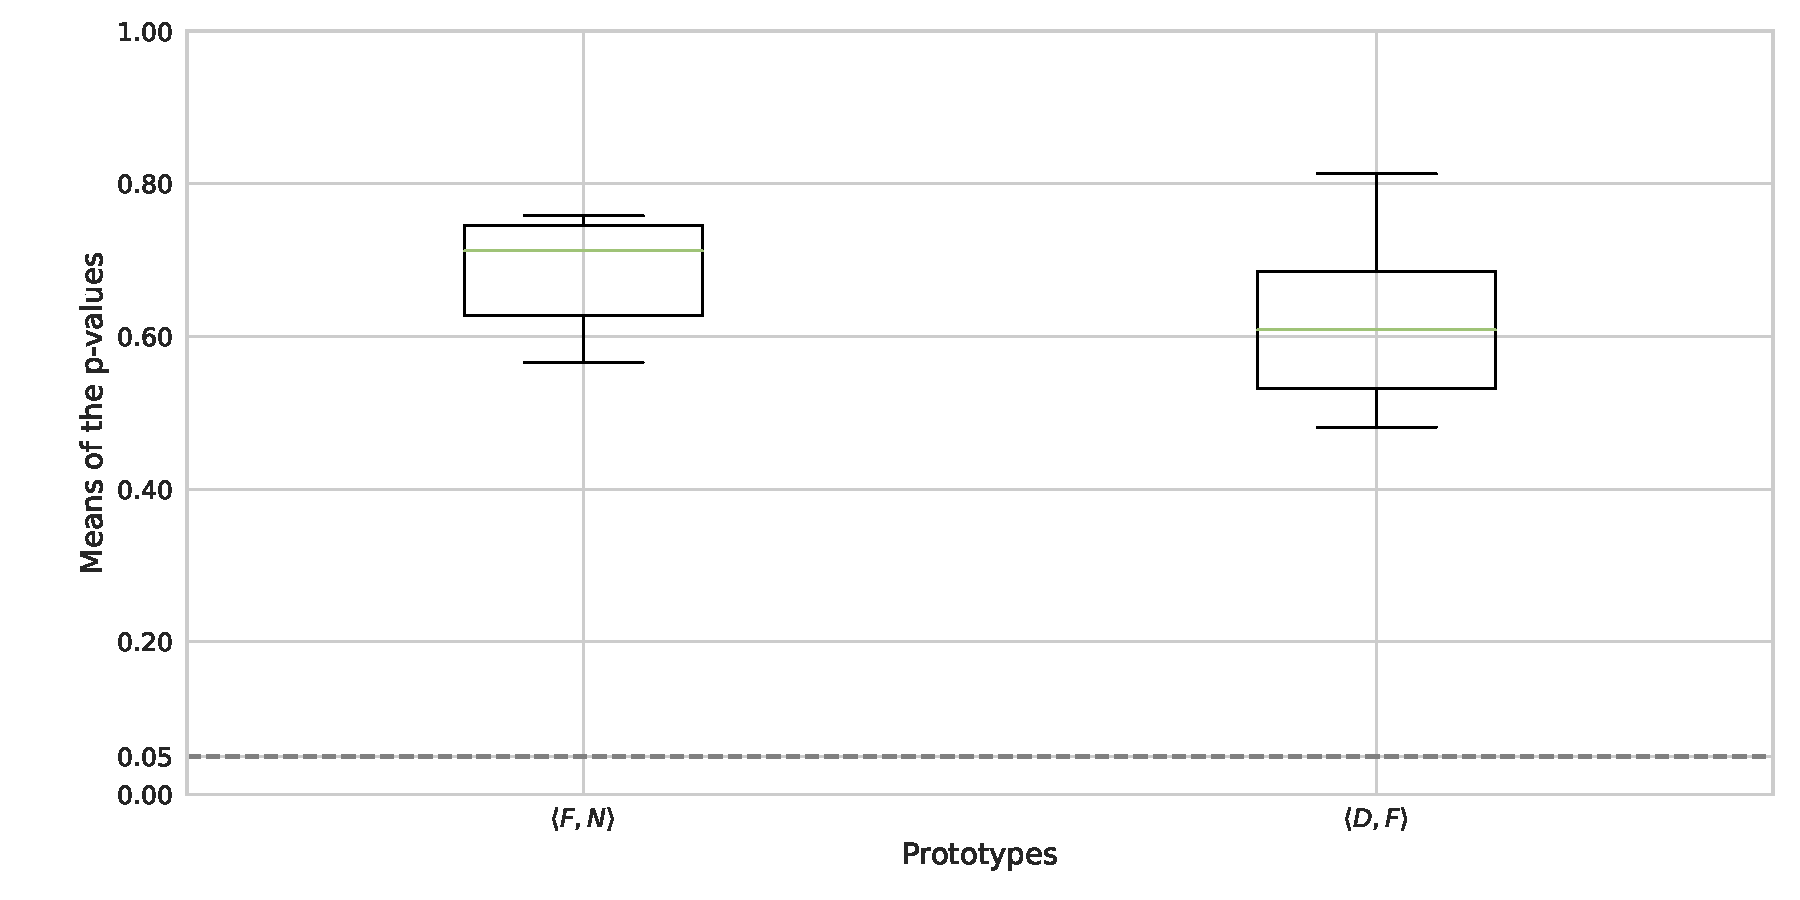
\includegraphics[width=0.9\textwidth]{chapters/data-centric/supervised/img/10_times_4_folds_cv.pdf}
	\caption{The distribution of the p-values obtained after repeating the chi-square test for 10 times, for the 10 times 4-fold cross-validation.}
	\label{effective-fig:10-times-4-cv}
\end{figure*}

\begin{table}[!t]
	\caption{
		Union of rules from \Cref{effective-tbl:rules}.
	}
	\renewcommand{\arraystretch}{0.3}
	\footnotesize
	\centering
	\label{effective-tbl:rules-union}
	\begin{threeparttable}
		\begin{tabular}{p{1cm}p{1cm}p{1cm}p{1cm}p{1cm}p{1cm}p{1cm}}
			\toprule
			& $\boldsymbol{E}$ & $\boldsymbol{N}$ & $\boldsymbol{D}$ & $\boldsymbol{I}$ & $\boldsymbol{R}$ & $\boldsymbol{F}$
			\\	\cmidrule[.1em]{1-7}
			$\boldsymbol{E}$ & \cellcolor{gray!25} & \texttt{1} & \texttt{1} & \texttt{0} & \texttt{1} & \texttt{1} \\	\cmidrule[.1em]{1-7}
			$\boldsymbol{N}$ & \texttt{0} & \cellcolor{gray!25}  & \texttt{X} & \texttt{0} & \texttt{1} & \texttt{1} \\	\cmidrule[.1em]{1-7}
			$\boldsymbol{D}$ & \texttt{0} & \texttt{X} & \cellcolor{gray!25} & \texttt{0} & \texttt{0} & \texttt{1} \\	\cmidrule[.1em]{1-7}
			$\boldsymbol{I}$ & \texttt{1} & \texttt{1} & \texttt{1} & \cellcolor{gray!25}  & \texttt{1} & \texttt{1} \\	\cmidrule[.1em]{1-7}
			$\boldsymbol{R}$ & \texttt{0} & \texttt{0} & \texttt{0} & \texttt{0} & \cellcolor{gray!25}  & \texttt{0} \\	\cmidrule[.1em]{1-7}
			$\boldsymbol{F}$ & \texttt{0} & \texttt{0} & \texttt{0} & \texttt{0} & \texttt{0} & \cellcolor{gray!25} \\	\cmidrule[.1em]{1-7}
		\end{tabular}
		\begin{tablenotes}
			\scriptsize
			\item$\boldsymbol{E}$ - Encoding; $\boldsymbol{N}$ - Normalization; $\boldsymbol{D}$ - Discretization; $\boldsymbol{I}$ - Imputation; $\boldsymbol{R}$ - Rebalancing; $\boldsymbol{F}$ - Feature Engineering. \item \texttt{1} - a precedence edge exists between the row and the column, \texttt{0} - a precedence edge does not exist between the row and the column, \texttt{X} - the combination is meaningless.
		\end{tablenotes}
	\end{threeparttable}
\end{table}

\subsection{Effective Prototypes Composition}
\label{effective-ssec:composition}

In this, we foresee the composition of the previously defined rules (i.e., for the pairs of pre-processing steps), to generate the final set of rules that would allow to compose longer chains---consisting of more than two steps.
This is when we also resolve the inconsistencies and define precedences for the pairs of steps that may not have any precedence defined already---in that case, we basically take into account all the permutations.
This allows to finally generate the possible effective  prototypes.

\paragraph{Use case}
To generate the final prototypes, in this phase, we combine all the matrices generated by the previous steps.
That is, we take the union of the edges (represented by \texttt{1}'s) from the matrices in \Cref{effective-tbl:rules} (a,b,c), and create a new final adjacency matrix, shown in \Cref{effective-tbl:rules-union}.
This is the matrix that will allow us to generate the final effective prototypes.

Observing the table, one can realize that for pairs $\{F,R\}$ and $\{R,D\}$, no precedence edges exist.
This means that these pairs are somewhat equally relevant from either direction (any order), and thus when generating the final prototypes, both options should appear.

For a better reading, in Figure~3.6, we visualize \Cref{effective-tbl:rules-union} in form of a graph, where nodes represent the pre-processing steps and the directed edges represent a precedence order between them.
Out of the graph, we generate the final prototypes by taking all the maximum length variations (ordered arrangements without repetition) of the nodes, respecting the precedence rules (i.e., not contradicting the direction of existing edges).
The result is the set of five prototypes shown in Table 3.7. This set consisting of \textit{compatible}, \textit{meaningful} and \textit{promising} pairs of transformations is the set of recommended \textit{effective pipeline prototypes}.


\begin{figure}
	\begin{floatrow}
	\ffigbox{
		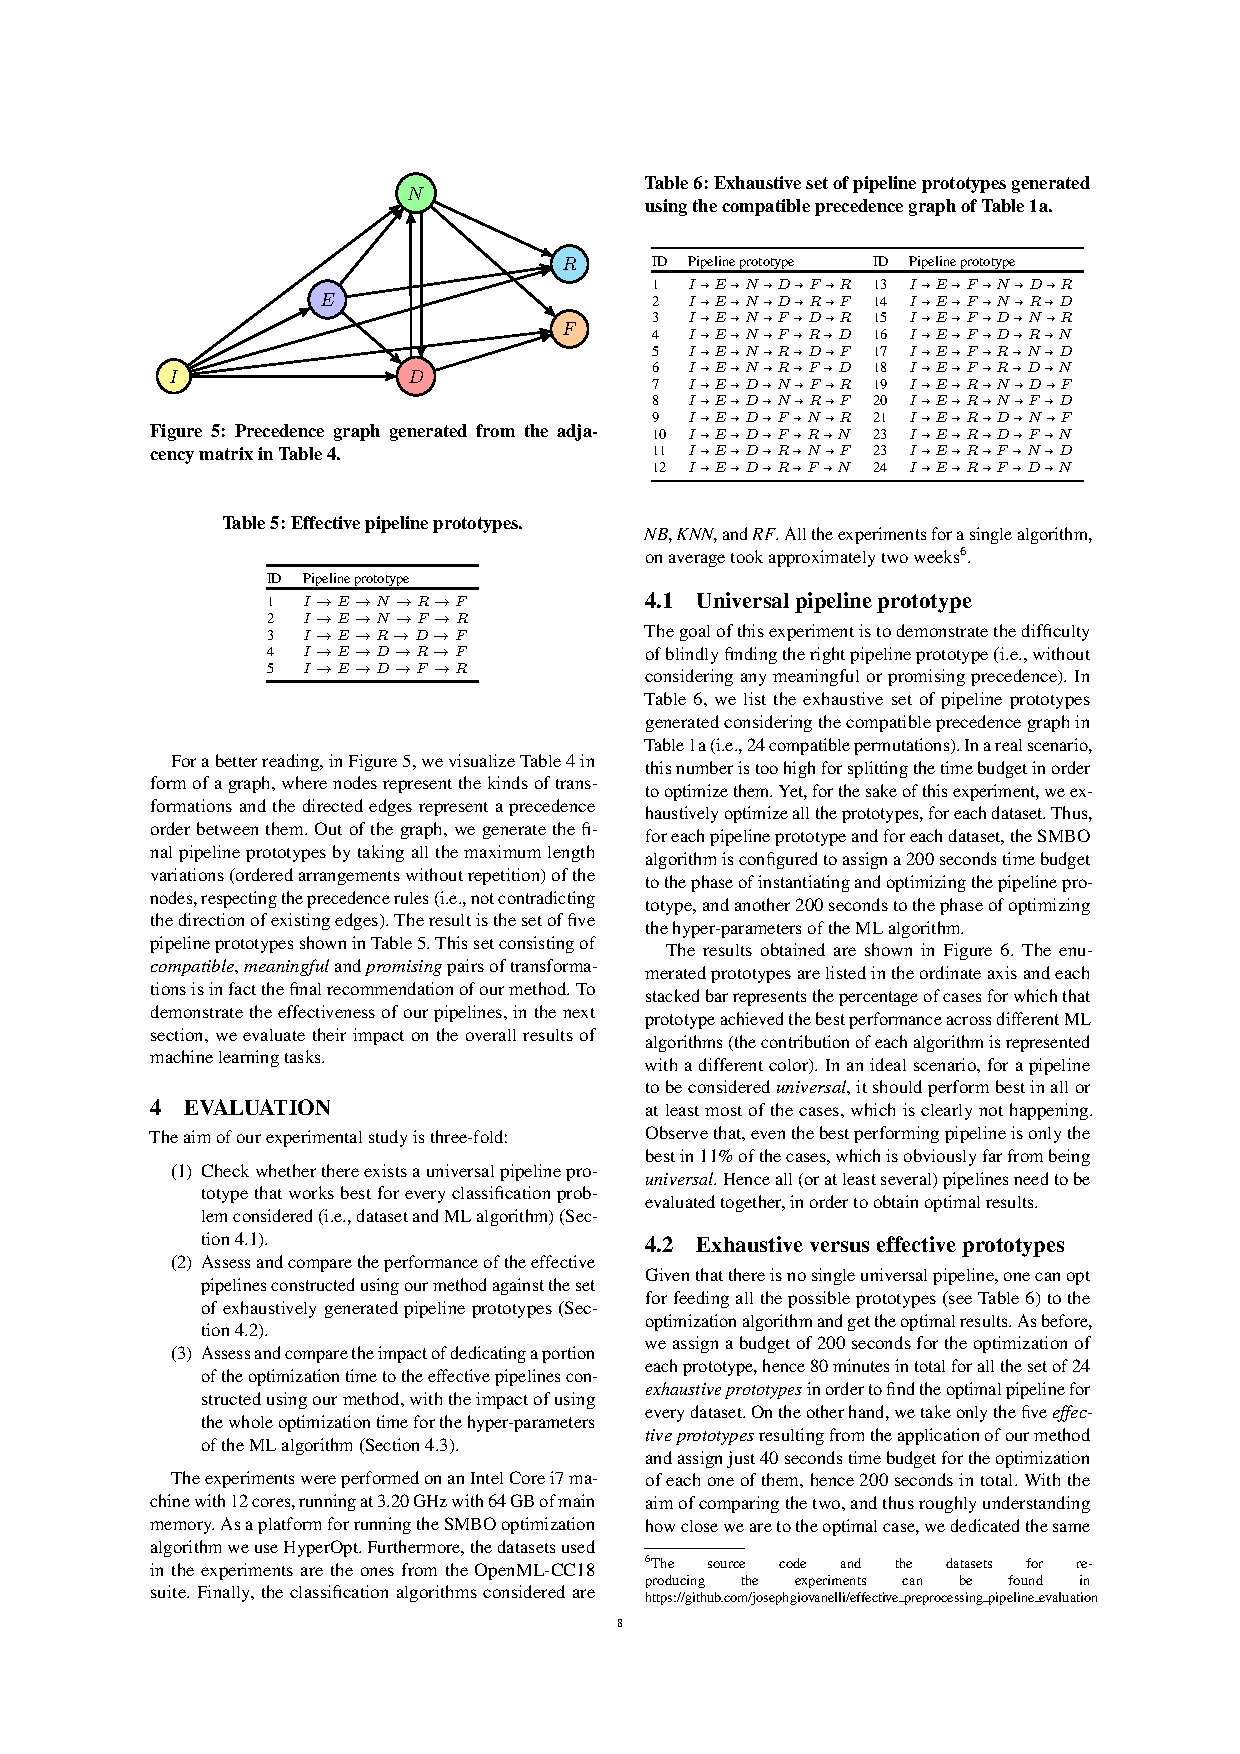
\includegraphics[clip, trim=2.5cm 23cm 10.5cm 2cm,width=0.5\textwidth]{chapters/data-centric/supervised/img/graph.pdf}
	}{
		  \caption{Precedence graph generated from \Cref{effective-tbl:rules-union}.}
	}
	\capbtabbox{
	\begin{tabular}{@{}ll}
				\toprule
				ID& Pipeline prototype                                             \\ \toprule
				1&{\color[HTML]{000000} $\langle I, E, N, R, F  \rangle$} \\
				2&{\color[HTML]{000000} $\langle I, E, N, F, R \rangle$} \\
				3&{\color[HTML]{000000} $\langle I, E, R, D, F \rangle$} \\
				4&{\color[HTML]{000000} $\langle I, E, D, R, F \rangle$} \\
				5&{\color[HTML]{000000} $\langle I, E, D , F, R \rangle$} \\
				\bottomrule
			\end{tabular}
	}{
		  \caption{Effective prototypes generated from Figure~3.6.
		}
	}
	\end{floatrow}
\end{figure}

\subsection{Meta-learning of Instantiation Rules}
\label{effective-ssec:meta-learning}

Once the pipeline prototypes are constructed (i.e., the order between the steps is defined), what follows is their instantiation with the actual transformations.
For that, one can rely completely on SMBO, and let the optimization choose the right transformation for each step.
However, as many optimization techniques, SMBO suffers from the cold-start problem where, in the beginning, it does not have enough information to come up with promising configurations, and a wrong choice may affect the whole process.

\subsubsection{Exploratory Analysis}
Given the availability of the experimental SMBO executions (executed in an exhaustive manner, considering all the prototypes), one can perform an exploratory analysis with the aim of removing useless prototypes, executable pipelines or sngle transformations.
Hence, further tweaking the search space.
In particular, one might analyze whether:

\begin{itemize}
    \item there exist some combination of steps (\Cref{effective-tbl:pipeline-enumeration}), that are generally useless (i.e., in terms of their impact on the final performance), and thus can be discarded a priori to reduce the search space;
    \item there are some executable pipelines that are consistently chosen more often than others by the optimization, meaning that they are more useful than others;
    \item within the executable pipelines, some transformations are chosen more often than others, meaning that they provide a more positive impact.
    \end{itemize}

\paragraph{Use case}
We performed the above-mentioned analysis, but this did not lead to any conclusive or significant results.
In particular, as shown in \Cref{effective-fig:prototypes-impact}, we could not find any useless prototypes---not positively impacting the final accuracy, that could be discarded a priori from the potential list of prototypes.
Actually, as we will show in \Cref{effective-sec:eval-universal-pipeline}, all of them lead to the best in one case or another, which does not mean the epsilon improvement some provide is worth the search cost you incur in considering them (but this more in-depth analysis is done later).
Next, as shown in \Cref{effective-fig:pipeline-frequency}, there were no physical pipelines shown to be more useful---hence more often selected, than others.
Even if $\langle N , R \rangle$ is clearly above, it barely reaches 30\% in KNN.
Finally, observing \Cref{effective-fig:transformation-frequency}, it is clear that some kinds of transformations are chosen more often, but looking closely (i.e., the shaded bars), it is not clear which operator brings more benefit.
For instance, Normalization is present in 90\% of the pipelines, but it is not easy to distinguish which kind of Normalization (i.e., actual operator) is more beneficial.
For this, we need more complex rules or guidelines that may help in finding the right operator to use.


\begin{figure*}[!t]
	\centering
	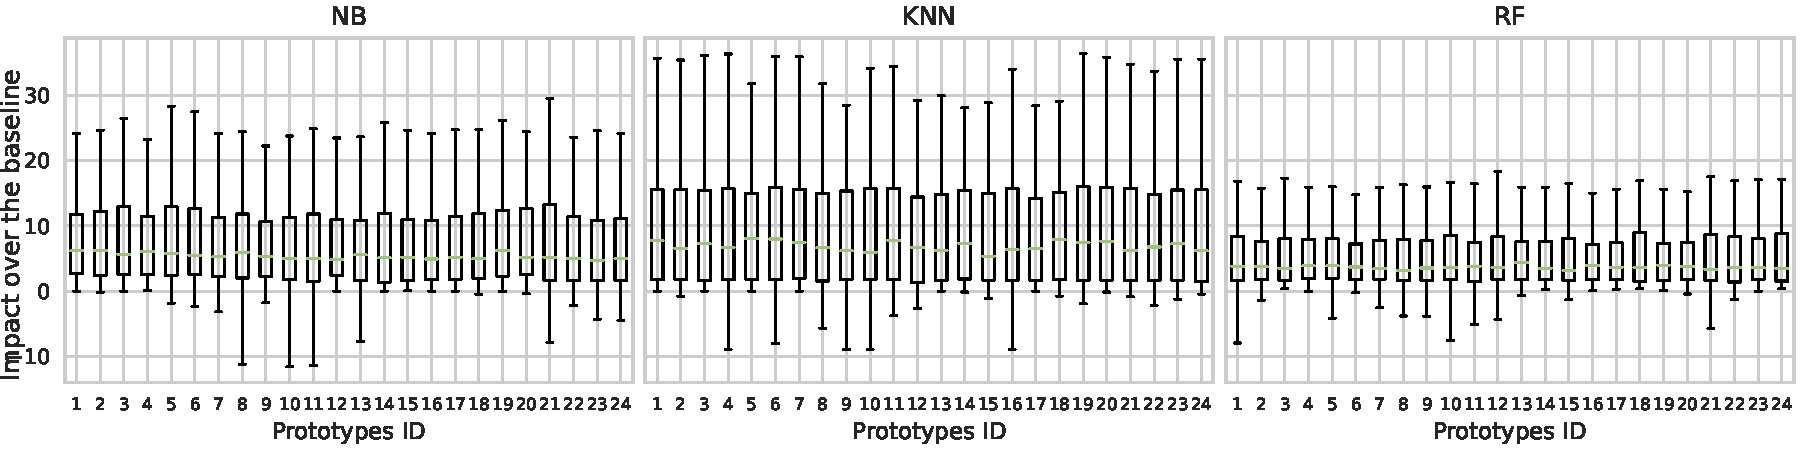
\includegraphics[width=1.0\textwidth]{chapters/data-centric/supervised/img/prototypes_impact.pdf}
	\caption{The impact of the different pipeline prototypes over the baseline (i.e., when no transformation is applied).}
	\label{effective-fig:prototypes-impact}
\end{figure*}

\begin{figure*}[!h]
	\centering
	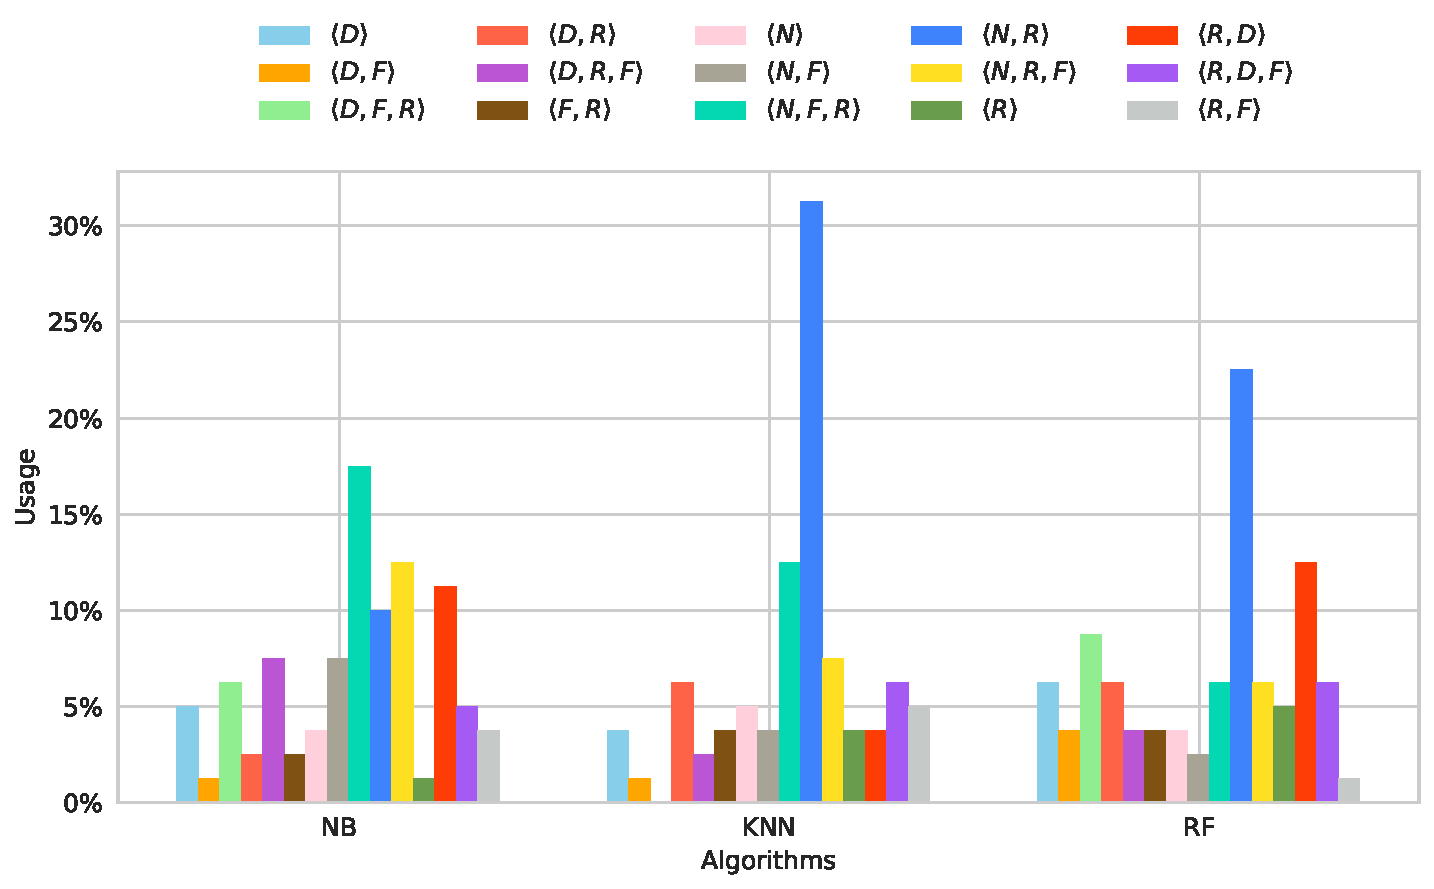
\includegraphics[width=1.0\textwidth]{chapters/data-centric/supervised/img/pp_pipeline_study2.pdf}
	\caption{Percentage of use of the different physical pipelines.}
	\label{effective-fig:pipeline-frequency}
\end{figure*}

\begin{figure*}[!h]
	\centering
	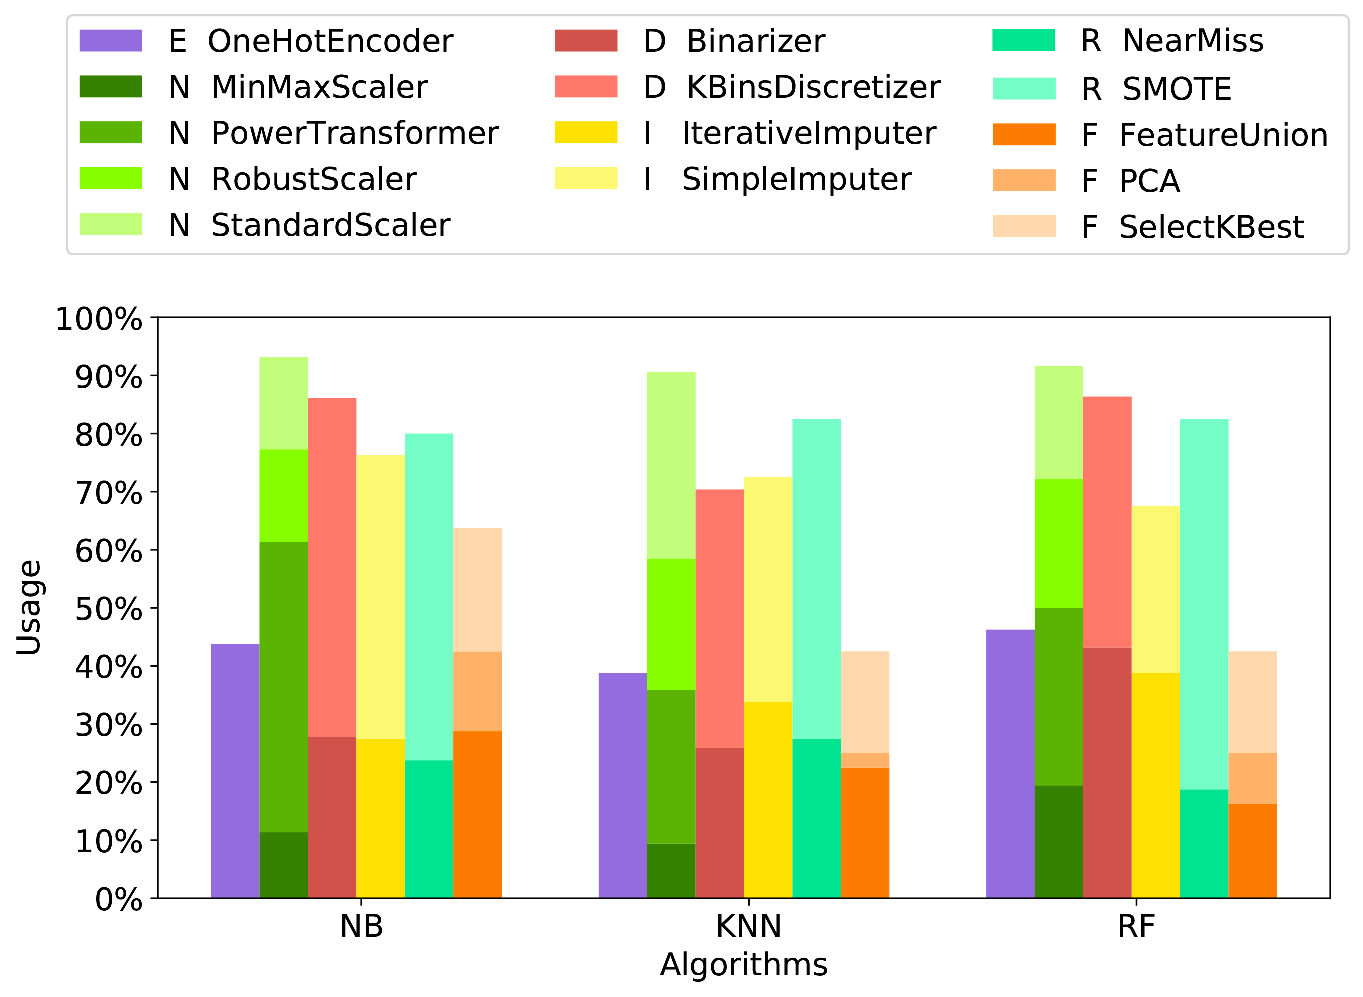
\includegraphics[width=0.7\textwidth]{chapters/data-centric/supervised/img/pp_pipeline_study_grouped.pdf}
	\caption{Percentage of use of a transformation in a physical pipeline.}
	\label{effective-fig:transformation-frequency}
\end{figure*}

\subsubsection{Meta-learning}
To mitigate the cold-start problem, we propose to perform meta-learning, where we intend to use the knowledge extracted from historical data in order to devise rules that may help the optimization in its initial settings.
Meta-learning is the process of ``learning on top of learning'', or learning a model using historical data from ML experiments.
Traditionally, it has been used for predicting the performance (e.g., accuracy) of an algorithm on a given dataset.
That is, given some historical runs of the performance of classification algorithms over various datasets (i.e., meta-dataset: consisting of datasets characteristics as meta-features and the performance of the ML algorithm as the desired outcome in a regression task), one can learn a model (i.e., meta-model), that is able to predict the performance of a given ML algorithm on a new dataset \cite{Brazdil04Book}.
Lately, this technique has been extended in order to predict the impact of pre-processing steps over the performance of ML algorithms and thus rank them based on the impact \cite{Bilalli17AMCS, presistant18CSI, presistant19DKE}.
The same idea can be applied to learning the best trnasformation for a given step.
That is, through meta-learning one can learn the intrinsic relationship between dataset characteristics and the transformation performance, and thus come up with rules that are not obvious and are effective at the time of pipeline instantiation.
The main idea is to build a model, that is able to predict the transformation for a certain pre-processing step, given the meta-features extracted from the dataset considered for the optimization.
This translates to answering the following question: ``given that we know the dataset characteristics and having selected a certain pre-processing step (e.g., Imputation), what is the optimal transformation we need to obtain the highest improvement w.r.t. loss (i.e., when the ML algorithm is applied over the transformed dataset)?''.
In particular, the model can generate a set of complementary rules that help in the optimization, providing a good starting instantiation for some of the steps in the prototype.

To train the model we need a meta-dataset that can be  (i) generated through optimization algorithms (e.g., SMBO executions), (ii) generated manually through simple evaluations of classification algorithms over transformed datasets, or (iii) assumed already given (e.g., OpenML).
Given a meta-dataset, we propose to learn to predict the best instantiation (transformation) for a given pre-processing step, including skipping the step (class \texttt{None}).

\paragraph{Use case}
Our training dataset for the meta-learning (i.e., meta-dataset) is built through SMBO runs on the OpenML datasets (\Cref{effective-ssec:rules-learned}).
We first extract the dataset characteristics (i.e., meta-features; e.g., number of features, number of instances, number of missing values).
Then, by applying SMBO optimization on classification algorithms and pre-processing prototypes, for each dataset, we retrieve the loss (in our case, accuracy) of the ML algorithms over the optimized pipelines.
This gives us the optimized executable pipelines and their impact on the accuracy of the learning algorithms for each dataset at hand.
Given such information, our aim is to now save time and improve the instantiation of the transformations for each step considered in the prototype.

We trained several different conditional inference trees (i.e., a particular implementation of decision trees \cite{ctree}) because they produce models that can be easily read and interpreted.
Specifically, the independence of each meta-feature with the class (transformation of a specific step) is tested through a statistical test.
The split is made on the variable with the lowest p-value.
We report the p-value too so that it can be seen how strong the association is (i.e., why that variable was chosen).
We stick with the p-value threshold of $0.05$, and devise a rule from any branch of the tree that is within the threshold.
In the following, we describe the rules obtained within the selected significance threshold.


\begin{figure}[!h]
	\centering
	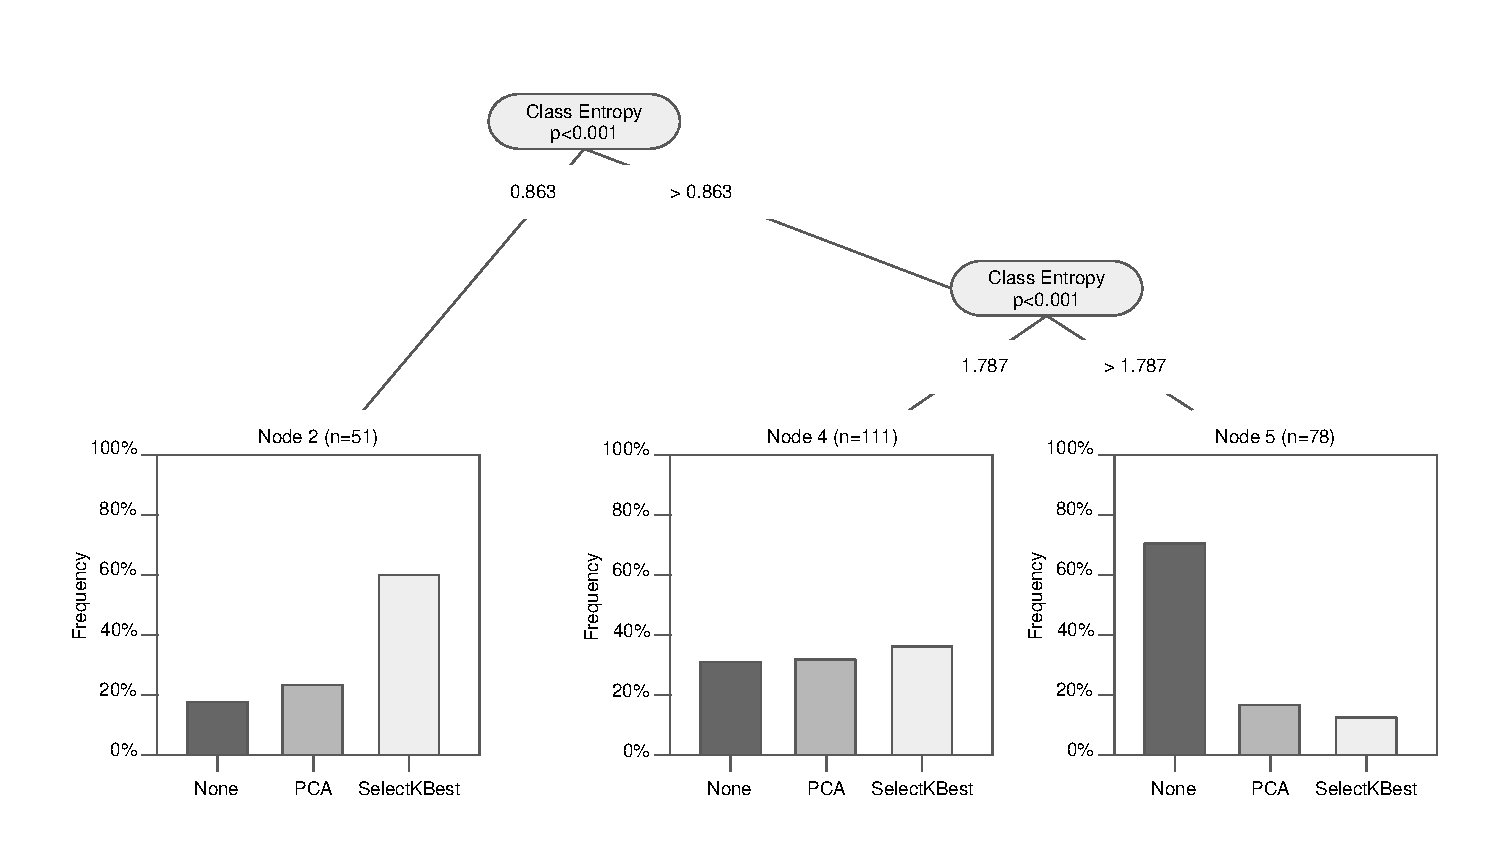
\includegraphics[clip, trim=1.0cm 0.4cm 1cm 1cm,width=1\textwidth]{chapters/data-centric/supervised/img/tree-FE.pdf}
	\caption{Conditional Inference Tree built for the \textit{Features Engineering} transformation.}
	\label{effective-fig:features-meta-learning:feature-engineering}
\end{figure}

\textbf{Rules for Feature Engineering}. The available transformations in scikit-learn for Feature Engineering are: Principal Component Analysis (\texttt{PCA}), \texttt{Feature Selection} (Select K Best), \texttt{Both} (PCA + Select K Best), and \texttt{None}.
The tree generated for the Feature Engineering transformation is shown in \Cref{effective-fig:features-meta-learning:feature-engineering}.
The leaves show the selected transformation frequency.
For the sake of simplicity, we do not consider the union of PCA and Select K Best as a transformation per se, instead we distribute that contribution to the two operators that compose it.
Observe that there is a strong correlation between the Feature Engineering transformation and the entropy of the class.
Indeed, such a meta-feature achieved a p-value smaller than $0.001$.
We can clearly read that if the Class Entropy is low, then \texttt{Feature Selection} is way more chosen than the other options (see Node 2).
Recall that entropy is a measure of how much disorder there is in its domain.
The less is that value, the easier is the classification problem.
As a consequence, it is reasonable to think that the easier the classification problem is, the more likely is the fact that the class can be described by a low number of features.
Hence, the \texttt{Feature Selection} technique can be successfully applied.
Conversely, Node 5 shows that, when the Class Entropy is high, it is better to not apply any Feature Engineering operator.
As a matter of fact, a high value of Class Entropy involves a high number of classes and/or few instances per class, hence a really difficult problem.
In such cases, reducing the dimensionality of the dataset does not lead to any improvement.
Finally, when the Class Entropy is in between, there is no clear winner, and thus other non-obvious factors may affect the choice of the operator.

\begin{figure}[!h]
	\centering
	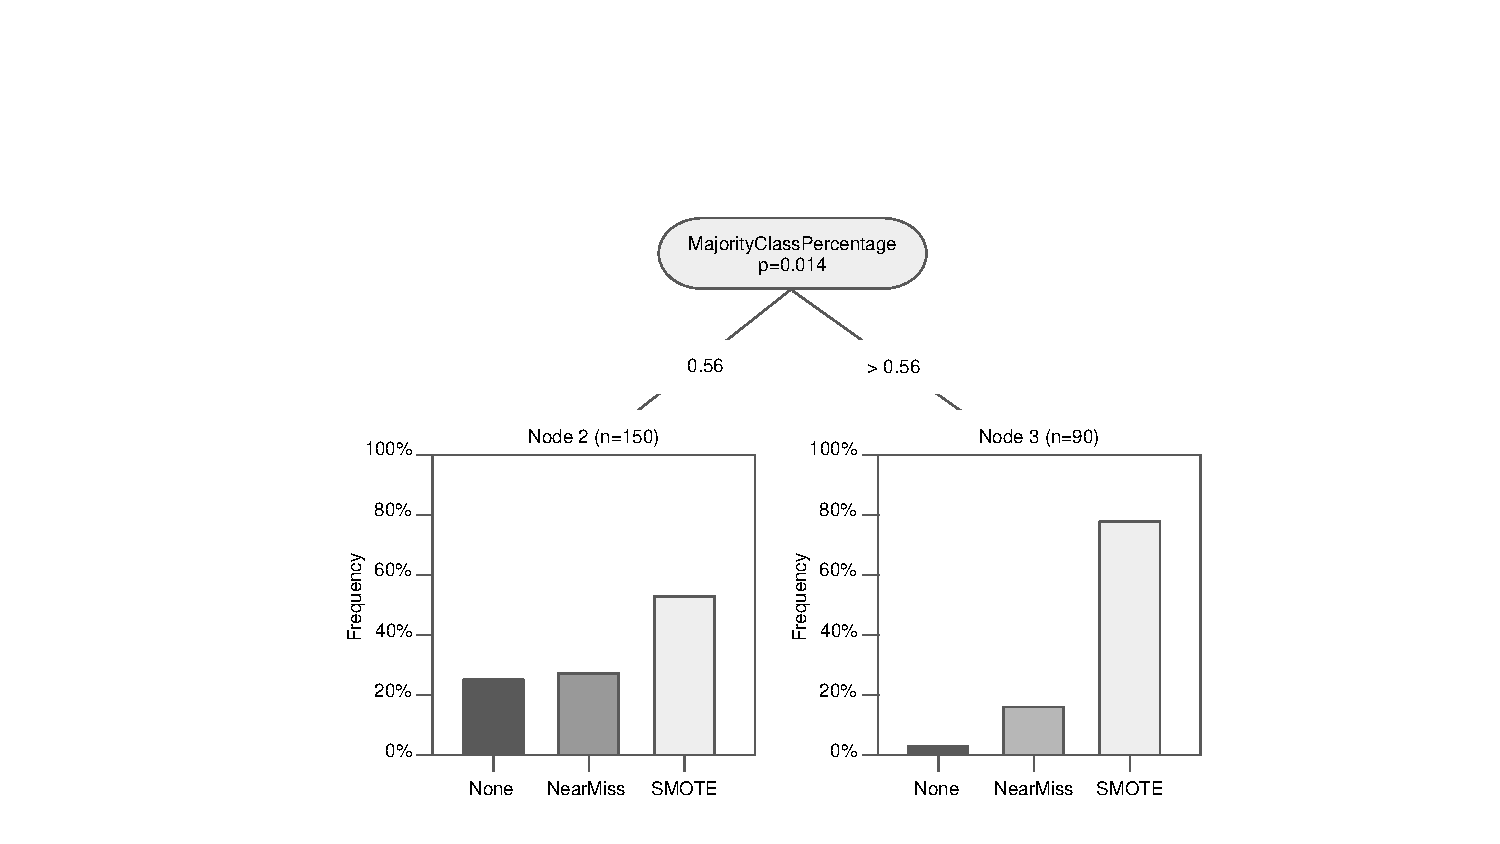
\includegraphics[clip, trim=5.8cm 0.4cm 5.05cm 3.5cm,width=0.65\textwidth]{chapters/data-centric/supervised/img/tree-RE.pdf}
	\caption{Conditional Inference Tree built for the \textit{Rebalancing} transformation.}
	\label{effective-fig:features-meta-learning:rebalancing}
\end{figure}

\textbf{Rules for Rebalancing}. As for Rebalancing, the transformations considered from the imblearn\footnote{\url{https://pypi.org/project/imbalanced-learn}} library are: \texttt{Near Miss}, \texttt{SMOTE}, and \texttt{None}.
The first is an undersampling algorithm which randomly eliminates the samples from the larger class; the second is an oversampling technique that creates samples of the minority class, as a linear combination of them.
As shown in \Cref{effective-fig:features-meta-learning:rebalancing}, the meta-feature Majority Class Percentage has a p-value of $0.014$.
This can be read as, in case of an unbalanced class problem (i.e., Node 3: Majority Class Percentage greater than 56), an oversampling of the minority class(es) is preferred to a downsampling of the majority one(s).
However, when the Majority Class Percentage is smaller than 56\%, the situation is not that clear, and there is no technique that is applied significantly more often than the rest; they are close to each other.
Therefore, it is difficult to understand which problems (which dataset characteristics do they have) belong to Node 2.
In summary, when the majority class has no more than 56\% , it implies that it is an unbalanced class, and as mentioned above, SMBO tends to choose the same transformation.
However, when the majority class has less than 56\%, it may imply that: (i) there are just two classes and the problem counts as a balanced problem, so no transformation needs to be applied, or (ii) it is a multi-class problem, and thus there is no clear winner in terms of transformation.

\subsection{Data Pipeline Instantiation}
\label{effective-ssec:prototype-insta}

The prototypes from the top flow and the meta-lerning rules from the bottom flow (if the optimization framework permits) are finally fed to the final phase which deals with the instantiation and optimization of the prototypes. In this, we run SMBO until an optimized pipeline is found.

\paragraph{Use case}
 In our final execution, we run SMBO to find a suitable instantiation for the suggested prototypes. The simple but not obvious meta-learning rules, even though not included in our final execution, because of the implementation considered (i.e., HyperOpt), can potentially be used to ease the cold-start problem.

\section{Empirical Evaluation}
\label{effective-sec:evaluation}


The aim of our experimental study is three-fold:
\begin{enumerate}
    \item Check whether there exists a universal prototype that works best for any classification problem considered  (i.e., dataset and ML algorithm) (\Cref{effective-sec:eval-universal-pipeline}).
    \item Assess and compare the performance of optimizing the effective prototypes constructed using our method against the set of exhaustively generated prototypes (\Cref{effective-sec:eval-our-vs-rest}).
    \item Assess and compare the impact of dedicating a portion of the optimization time to the effective prototypes against using the whole optimization time for the hyperparameters of the ML algorithm (\Cref{effective-sec:eval-dpso-vs-cash}).
\end{enumerate}

The experiments were performed on an Intel Core i7 machine with 12 cores, running at 3.20 GHz with 64 GB of main memory.
We leveraged the SMBO optimization algorithm available in the Python library HyperOpt \cite{bergstra2015hyperopt}.
The datasets used in the experiments are the ones from the OpenML CC-18 repository \cite{OpenML2013}.
Finally, the classification algorithms considered are \textit{NB}, \textit{KNN}, and \textit{RF} from the Python library Scikit-learn \cite{scikit-learn}.
All the experiments for a single algorithm took approximately two weeks.


\paragraph{AutoPrep}
With the recent shift towards data-centric approaches, rather than algorithmic, data pre-processing is receiving a lot of attention.
Yet, its impact on the final analysis is not widely recognized, primarily due to the lack of publicly available experiments that quantify it.
To bridge this gap, along with this work, we contribute to publishing a companion reproducibility paper \cite{Giovanelli2022IS} for the experiments and results reported in the following.
AutoPrep introduces a set of reproducible experiments on the impact of data pre-processing by providing a detailed reproducibility protocol together with a software tool and a set of extensible datasets, which allow for all the experiments and results of this chapter reproduced.
Our experiments have been performed among different machines with different resources.
We achieved to deploy \textit{strongly reproducible experiments}, when based on a collection of intermediate results, and \textit{weakly reproducible experiments} when reproducing our end-to-end optimization from scratch.
The reproducibility protocol is created in Docker and tested in Windows and Linux.
The source code and the datasets for reproducing the experiments can be found on GitHub\footnote{
\url{https://github.com/josephgiovanelli/autoprep}}.

\begin{definition}[Strongly reproducible experiment  \cite{reproducible}]
    \label{def:strong}
    Given a set of previously reported experimental results and conclusions, a computational experiment is strongly reproducible if it allows to confirm both previously reported results and conclusions exactly.
\end{definition}

\begin{definition}[Weakly reproducible experiment  \cite{reproducible}]
    \label{def:weak}
    Given a set of previously reported experimental results and conclusions, a computational experiment is weakly reproducible if the Spearman rank correlation between the original and reproduced results is equal to 1, and their Pearson correlation value is high enough to allow the confirmation of all previously reported conclusions, even if the reproduced results do not reproduce all results exactly. Thus, weak reproducibility is a performance-rank-preserving notion.
\end{definition}

\subsection{Universal Pipeline Prototype}
\label{effective-sec:eval-universal-pipeline}
The goal of this experiment is to demonstrate the difficulty of blindly finding the right prototype (i.e., without considering any meaningful or promising precedence).
In \Cref{effective-tbl:pipeline-enumeration}, we list the exhaustive set of pipeline prototypes generated considering the compatible precedence graph in Table~\ref{effective-tbl:rules}a (i.e., 24 compatible permutations).
In a real scenario, this number would be too high for splitting the time budget in order to optimize them.
Yet, for the sake of this experiment, we exhaustively optimize all the prototypes, for each dataset.
Thus, for each prototype and for each dataset, the SMBO algorithm is configured to assign a 200 seconds time budget to the phase of instantiating and optimizing the prototype, and another 200 seconds to the phase of optimizing the hyperparameters of the ML algorithm.

\begin{table}[t]
\caption[Enumeration of the prototypes that can be generated by compatible precedence]{Exhaustive set of prototypes generated using the compatible precedence graph of Table~\ref{effective-tbl:rules}a. $E$ - Encoding; $N$ - Normalization; $D$ - Discretization; $I$ - Imputation; $R$ - Rebalancing; $F$ - Feature Engineering.
}
\footnotesize
\label{effective-tbl:pipeline-enumeration}
\begin{center}
\begin{tabular}{@{}lllll@{}}
\toprule
ID & Pipeline prototype & ID & Pipeline prototype                                                                   \\ \toprule
1  & {\color[HTML]{000000} $\langle I, E, N, D, F, R \rangle$} & 13 & {\color[HTML]{000000} $\langle I, E, F, N, D, R \rangle$} \\
2  & {\color[HTML]{000000} $\langle I, E, N, D, R, F \rangle$} & 14 & {\color[HTML]{000000} $\langle I, E, F, N, R, D \rangle$} \\
3  & {\color[HTML]{000000} $\langle I, E, N, F, D, R \rangle$} & 15 & {\color[HTML]{000000} $\langle I, E, F, D, N, R \rangle$} \\
4  & {\color[HTML]{000000} $\langle I, E, N, F, R, D \rangle$} & 16 & {\color[HTML]{000000} $\langle I, E, F, D, R, N \rangle$} \\
5  & {\color[HTML]{000000} $\langle I, E, N, R, D, F \rangle$} & 17 & {\color[HTML]{000000} $\langle I, E, F, R, N, D \rangle$} \\
6  & {\color[HTML]{000000} $\langle I, E, N, R, F, D \rangle$} & 18 & {\color[HTML]{000000} $\langle I, E, F, R, D, N \rangle$} \\
7  & {\color[HTML]{000000} $\langle I, E, D, N, F, R \rangle$} & 19 & {\color[HTML]{000000} $\langle I, E, R, N, D, F \rangle$} \\
8  & {\color[HTML]{000000} $\langle I, E, D, N, R, F \rangle$} & 20 & {\color[HTML]{000000} $\langle I, E, R, N, F, D \rangle$} \\
9  & {\color[HTML]{000000} $\langle I, E, D, F, N, R \rangle$} & 21 & {\color[HTML]{000000} $\langle I, E, R, D, N, F \rangle$} \\
10 & {\color[HTML]{000000} $\langle I, E, D, F, R, N \rangle$} & 23 & {\color[HTML]{000000} $\langle I, E, R, D, F, N \rangle$} \\
11 & {\color[HTML]{000000} $\langle I, E, D, R, N, F \rangle$} & 23 & {\color[HTML]{000000} $\langle I, E, R, F, N, D \rangle$} \\
12 & {\color[HTML]{000000} $\langle I, E, D, R, F, N \rangle$} & 24 & {\color[HTML]{000000} $\langle I, E, R, F, D, N \rangle$}
\\ \bottomrule
\end{tabular}
\end{center}
\end{table}

The results obtained are shown in \Cref{effective-fig:eval-universal-pipeline}.
The enumerated prototypes are listed in the abscissa axis and each stacked bar represents the percentage of cases for which that prototype achieved the best performance across different ML algorithms (the contribution of each algorithm is represented with a different color).
In an ideal scenario, for a prototype to be considered \textit{universal}, it should perform best in all or at least most of the cases, which is clearly not happening.
Observe that, even the best-performing prototype is only the best in 19\% of the cases, which is obviously far from being \textit{universal}.
Hence all (or at least several) prototypes need to be evaluated together, in order to obtain better solutions.

\begin{figure}[t]
    \centering
    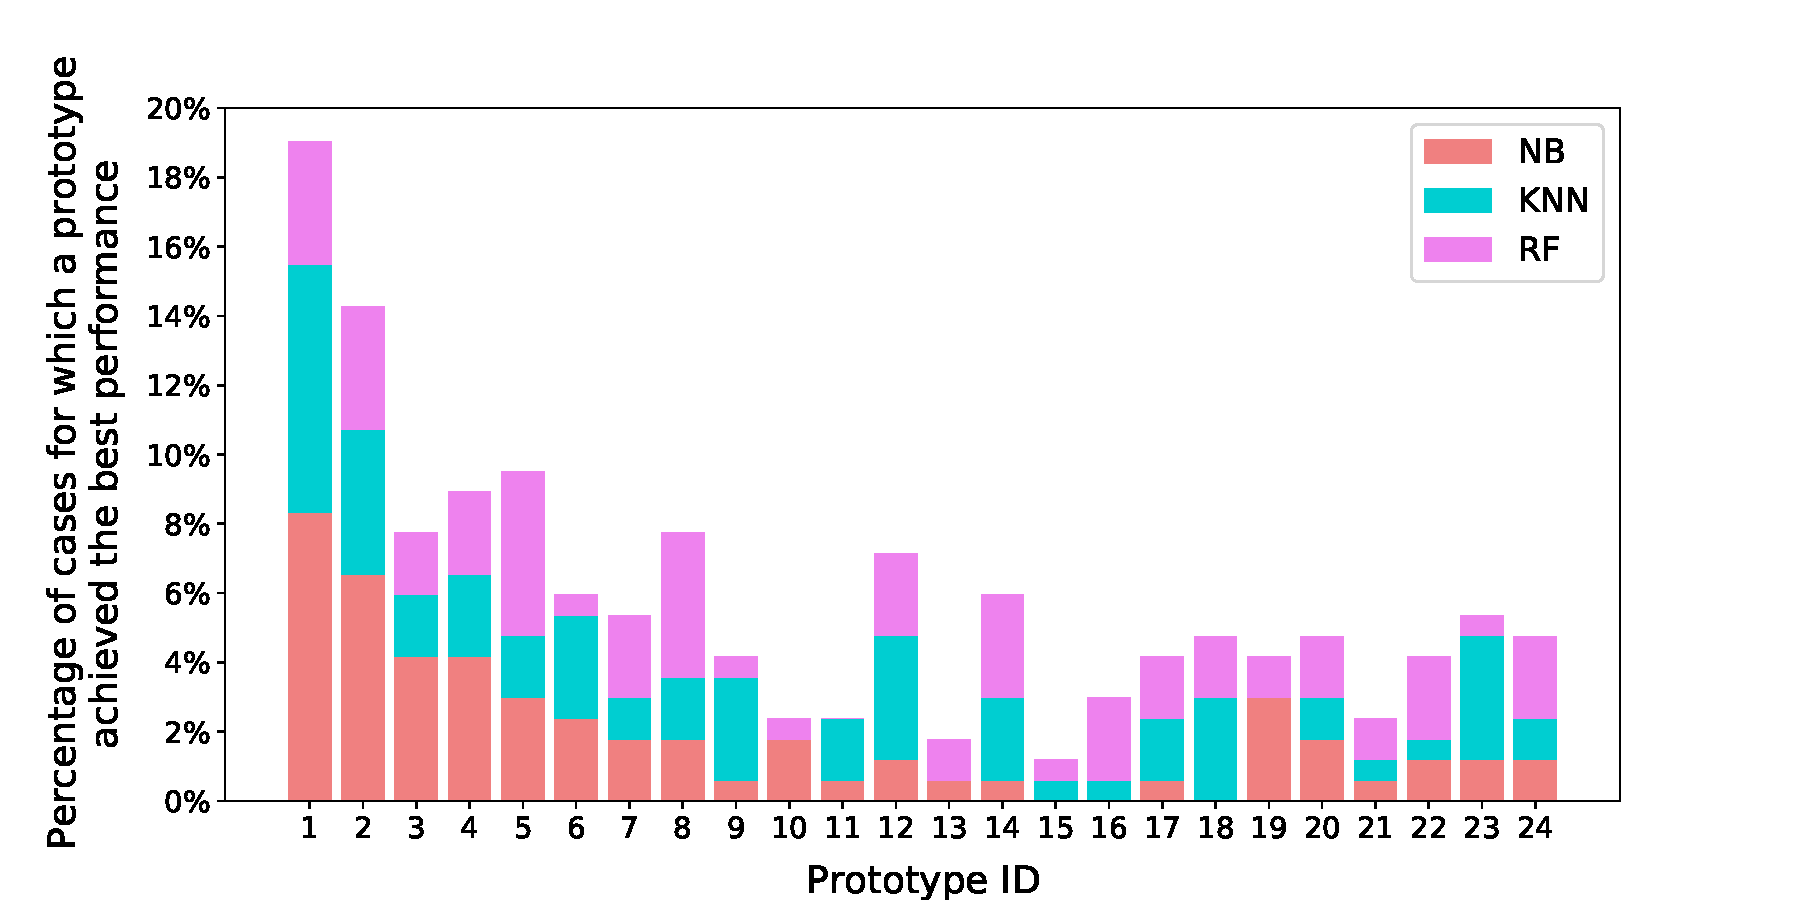
\includegraphics[width=0.8\textwidth]{chapters/data-centric/supervised/img/evaluation1.pdf}
    \caption{Comparison of the goodness of the exhaustive set of prototypes.}
    \label{effective-fig:eval-universal-pipeline}
\end{figure}

\subsection{Exhaustive Versus Effective Prototypes}
\label{effective-sec:eval-our-vs-rest}
Given that there is no single universal prototype, one can opt for feeding all the possible prototypes (see \Cref{effective-tbl:pipeline-enumeration}) to the optimization algorithm in order to get the best solutions out of them.
As before, we assign a budget of 200 seconds for the optimization of each prototype, hence 80 minutes in total for all the set of 24 \textit{exhaustive prototypes} in order to find the optimal pipeline for every dataset.
On the other hand, we take only the five \textit{effective prototypes} resulting from the application of our method and assign just 40 seconds time budget for the optimization of each one of them, hence 200 seconds in total. With the aim of comparing the two, and thus roughly understanding how close we are to the optimal case, in both cases, we dedicated the same time budget (i.e., 200 seconds) for the phase of optimizing the hyperparameters of the ML algorithm.
In order to evaluate how close the \textit{effective prototypes} are to the \textit{exhaustive ones}, we calculate the \textit{normalized distance} from the result to the optimum---w.r.t. accuracy.

\begin{equation*}
    normalized\;distance = \frac{ACC_{\textup{eff}} - ACC_{\varnothing}}{ACC_{\textup{exh}} - ACC_{\varnothing}}
\end{equation*}

$ACC_{\varnothing}$ is the baseline performance (i.e., accuracy of the algorithm $A$ with default hyperparameters and no data pipeline, hence computed over the original dataset $\altmathcal{D}$), formally $ACC_{\varnothing} = ACC( \langle \varnothing, A  \rangle (\altmathcal{D}_{train}), \altmathcal{D}_{valid})$.
$ACC_{\textup{eff}}$ is the accuracy of the optimized algorithm $A_{{\lambda}^{\star}}$ over the dataset transformed using the optimized instantiation of the effective set of prototypes (i.e., our approach), formally $ACC_{\textup{eff}} = ACC(\langle P^{\star}_{\textup{eff}_{{\lambda}^{\star}}}, A_{\lambda^\star} \rangle (\altmathcal{D}_{train}), \altmathcal{D}_{valid})$.
Finally, $ACC_{\textup{exh}}$ is the accuracy of the optimized algorithm $A_{{\lambda}^{\star}}$ over the dataset transformed using the optimized pipeline instantiation of the exhaustive set of prototypes, formally $ACC_{\textup{exh}} = ACC(\langle P^{\star}_{\textup{exh}_{{\lambda}^{\star}}}, A_{\lambda^\star} \rangle (\altmathcal{D}_{train}), \altmathcal{D}_{valid})$.
The subtraction by $ACC_{\varnothing}$ is done with the aim of weighting the difficulty of a dataset, hence allowing for comparisons in terms of the gain in accuracy.
To this end, the bigger the potential gain (denominator) is, the bigger the obtained gain (numerator) must be, for the latter to be relevant.

The results obtained for every dataset and algorithm are shown as boxplots in \Cref{effective-fig:eval-exhaustive-vs-effective}.
Observe that, most of the cases are very close to the results obtained using the exhaustive set, the median distances being 91.51\%, 93.13\%, 88.97\%, for NB, KNN, and RF, respectively.
In general, in 75\% of the cases the chosen pipelines are above 80\%, and only few outliers are below 60\%.
Curiously, in some cases, we outperform the results over the exhaustive set of pipelines, but this is due to the randomness of the optimization algorithm, which unless it is given an unrealistically high budget of time, is not capable of finding the true optimal solution.
We discarded the option of assigning a larger budget since this was not practical considering the huge search space and the lack of any guarantee of improvement.

To summarize, the experiment shows that with roughly 24 times less time budget, we can obtain results that are as good as 90\% in the median compared to the exhaustive ones.
The raw results (i.e., without the normalized distances) can be found on the aforementioned GitHub page.

\begin{figure}[!t]
    \centering
    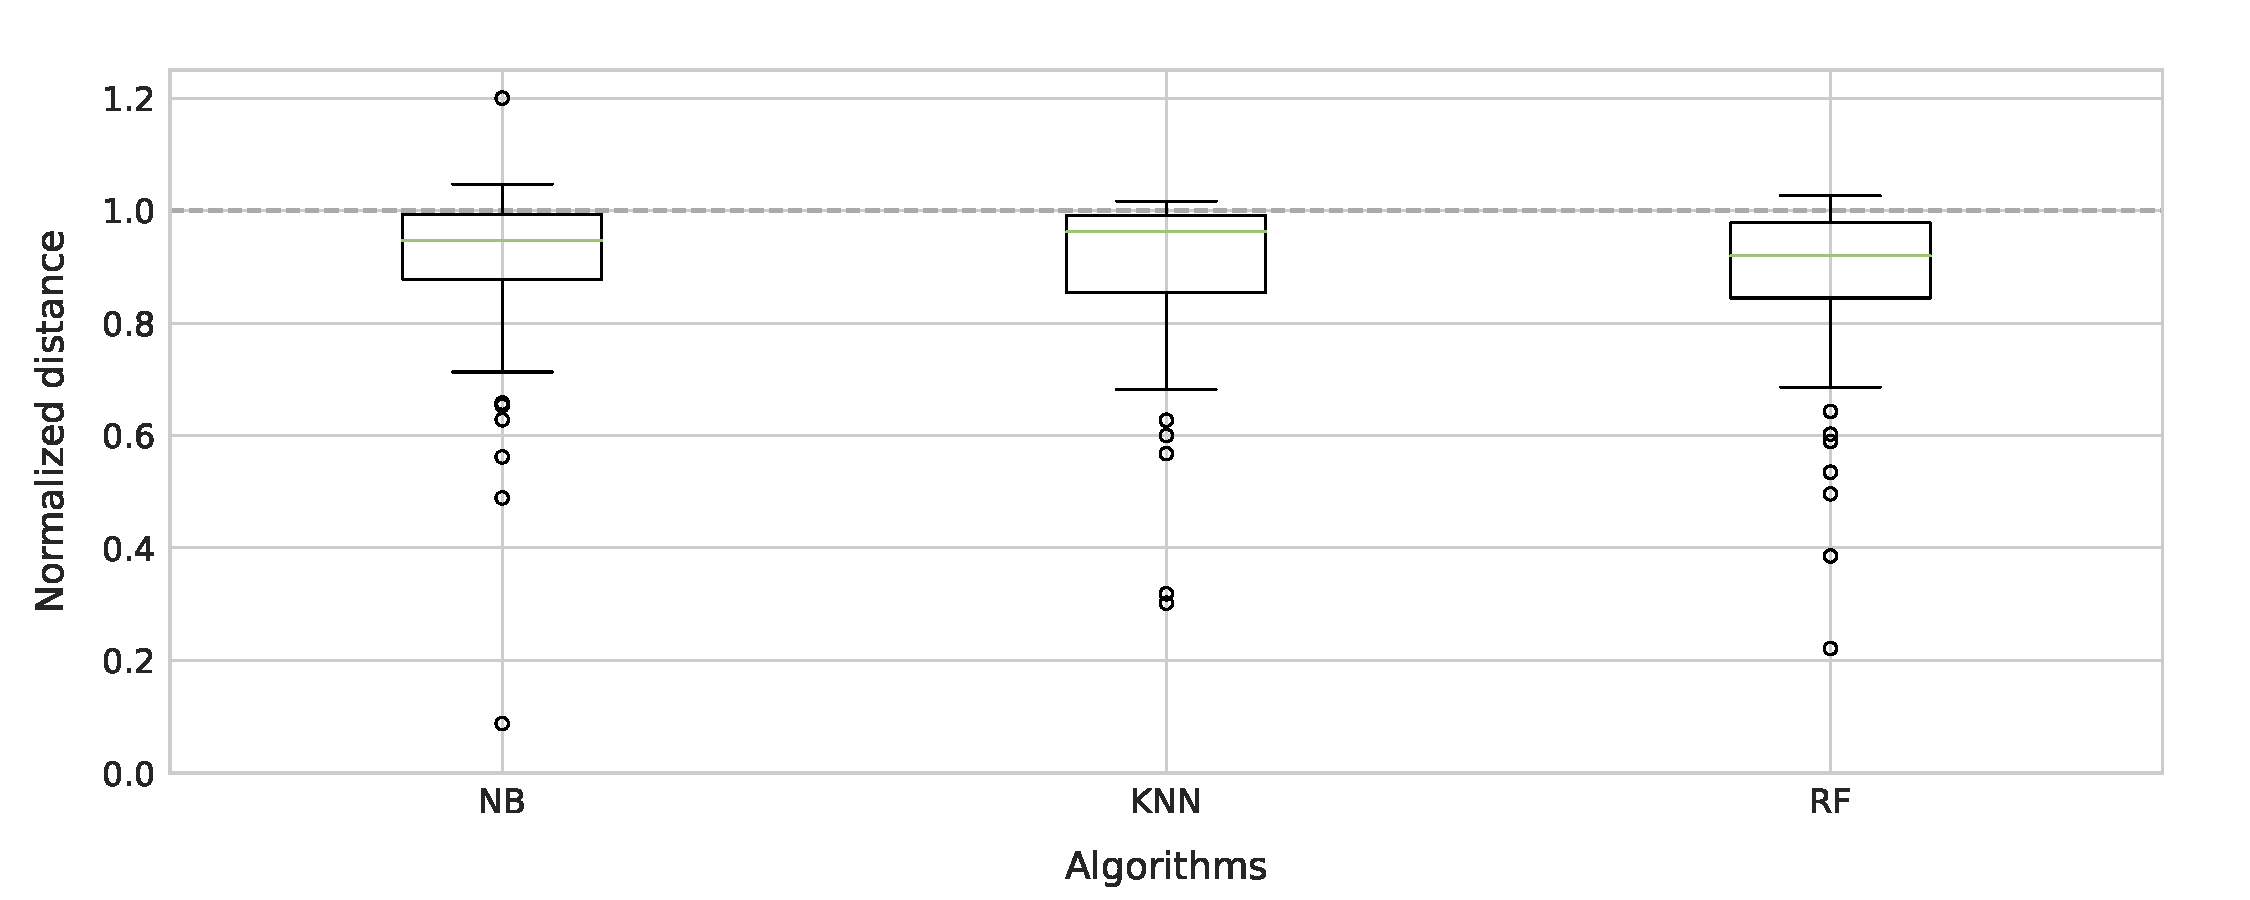
\includegraphics[width=1.0\textwidth]{chapters/data-centric/supervised/img/evaluation2.pdf}
    \caption{Normalized distances between the scores obtained by optimizing our effective prototypes and the ones obtained by optimizing the exhaustive set.}
    \label{effective-fig:eval-exhaustive-vs-effective}
\end{figure}

\subsection{Complementing HPO of ML algorithm with Pre-processing}
\label{effective-sec:eval-dpso-vs-cash}

\begin{figure*}[!t]
	\centering
	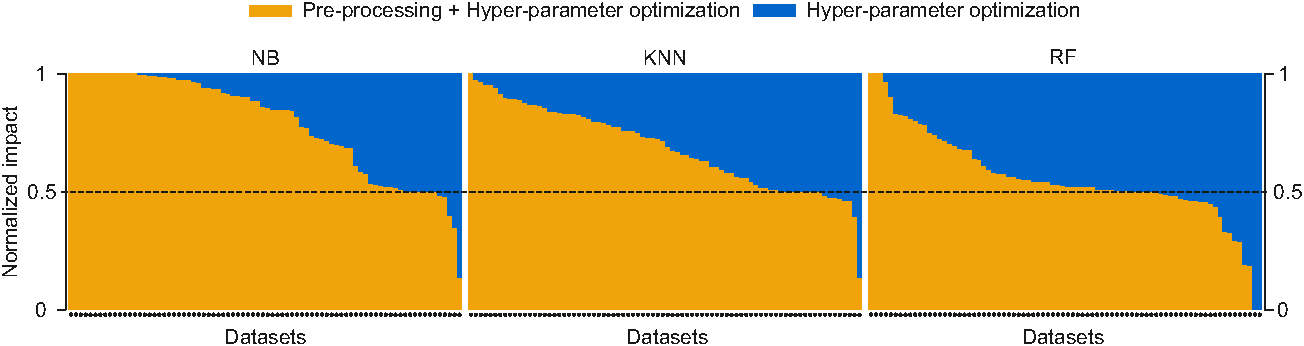
\includegraphics[width=1.0\textwidth]{chapters/data-centric/supervised/img/barplot-10.pdf}
	\caption{The impact of dedicating a portion of the optimization budget to pre-processing compared to using the whole optimization budget for the ML algorithm HPO.}
	\label{effective-fig:eval-pre-processing-hyperparameter}
\end{figure*}

We have just shown that our effective prototypes have similar impact as the exhaustive ones.
Now we want to compare the impact of the effective prototypes against optimizing only the hyperparameters of the ML algorithm.
That is, we want to examine whether dedicating a part of the optimization budget to the pre-processing impacts more (positively) the results of the analysis, than using the whole budget for solely the hyperparameter optimization of the ML algorithm\footnote{To enable the application of the ML algorithms on all the datasets, whenever required, we apply the necessary transformation (e.g, imputation or encoding).}---i.e., modelling.

To this end, for the latter we now dedicate the total optimization budget (i.e., 400 seconds), and for the former, inspired by \cite{Quemy20InfSystems}, we split the budget 50-50 between the pre-processing pipeline optimization and the hyperparameter optimization (i.e., 200 seconds for the pre-processing, and 200 seconds for the hyperparameter optimization).
The time for the pre-processing is further split among the five different pipeline prototypes (i.e., 40 seconds each).

To compare the results, we calculate the impact using the formulas below, which correspond to the normalized distance from either pre-processing or hyperparameter optimization to the maximum improvement that can be achieved, regardless of whether pre-processing is applied or not.

\begin{equation*}
    \text{\textit{pp impact}} = \frac{ACC_{\textup{eff}} - ACC_{\varnothing}}{max(ACC_{\textup{eff}}, ACC_{\textup{hpo}}) - ACC_{\varnothing}}
\end{equation*}

\begin{equation*}
    \text{\textit{hp impact}} = \frac{ACC_{\textup{hpo}} - ACC_{\varnothing}}{max(ACC_{\textup{eff}}, ACC_{\textup{hpo}}) - ACC_{\varnothing}}
\end{equation*}

$ACC_{\varnothing}$ is yet again the baseline performance (i.e., accuracy of the algorithm $A$ with default hyperparameters over the original dataset $\altmathcal{D}$).
$ACC_{\textup{eff}}$ is still the accuracy of our approach, i.e., the optimized algorithm $A_{{\lambda}^{\star}}$ with half of the whole budget over the dataset transformed using the optimized instantiation of the effective set of prototypes (with half of the whole budget).
Finally, $ACC_{\textup{hpo}}$ is the accuracy of the optimized algorithm $A_{{\lambda}^{\star}}$ (i.e, using the entire budget) over the original dataset, formally $ACC_{\textup{hpo}} = ACC( \langle A_{{\lambda}^{\star}} \rangle (\altmathcal{D}_{train}), \altmathcal{D}_{valid})$.

To obtain relative values that sum to 1, we normalize the impacts dividing them by their sum.
For instance, for the pre-processing score we calculate the following:
\begin{equation*}
    \text{\textit{normalized pp impact}} = \frac{\text{\textit{pp impact}}}
    {\text{\textit{pp impact}} + \text{\textit{hp impact}}}
\end{equation*}


We perform the same for the hyperparameter impact and plot the results obtained for all the algorithms and datasets in \Cref{effective-fig:eval-pre-processing-hyperparameter}, where each bar represents the results obtained for a single dataset.
The different colors represent the impact values of pre-processing and hyperparameter optimization.

Observing the bar charts one can see that (i) dedicating a portion of the budget to pre-processing, brings benefit to the analysis in most of the cases (i.e., $73\%$ of the cases), and (ii) the impact of hyperparameter optimization, increases with the increase of the number of hyperparameters of the ML algorithm (e.g., hyperparameter optimization impacts more RF than NB).
Overall, we can conclude that pre-processing is a critical step that once effectively applied may have a high positive impact on the final result of the analysis.

\section{Conclusions and Future Works}
\label{effective-sec:conclusions}

In this chapter, we first studied the overall impact of pre-processing steps when chained together inside prototypes and then delved into examining the impact of instantiating steps via various transformations.
As a result, we defined a method that allows to generate effective pre-processing pipelines.
That is, pipelines that consist of, (i) compatible pairs of steps concerning the framework used,  (ii) meaningful pairs of steps in terms of general knowledge (best practices), and (iii) promising pairs of steps that once applied are expected to provide higher overall impact (domain knowledge).
In addition, via the meta-learning phase proposed, we aim to guide the pipeline instantiation in order to facilitate finding better transformations.

An extensive evaluation on 80 datasets with heterogeneous characteristics, from sample size to feature types, and a set of classification algorithms (i.e., Naive Bayes, Random Forest, K-Nearest Neighbours), showed that our devised prototypes give promising results.
More specifically, we were able to observe that:
\begin{itemize}
    \item [--] The overall impact of optimizing pre-processing is not negligible and it may boost the performance of the overall analytics (e.g., accuracy).
    \item [--] There is no universal pre-processing prototype that works best for every dataset and algorithm.
    \item [--] With 24 times less time budget, our proposed prototypes were able to obtain results that were as good as 90\% in the median of the optimal ones found through an exhaustive search.
    \item [--] Dedicating a portion of the time to the pre-processing optimization, instead of dedicating it entirely to hyperparameter optimization may boost the final result of the analysis.
	On average, in 73\% of the cases including pre-processing in the optimization, outperformed the results of only optimizing hyperparameters.
\end{itemize}

The results indicate that pre-processing can boost the performance of the ML algorithm.
Hence, it must be considered as an integral part of the data analytics optimization process.

Finally, previous works have shown the effectiveness of meta-learning for solving the cold start problem \cite{Feurer15AAAI}, hence as immediate future work, we intend to extend an optimization framework (i.e., HyperOpt) with a complementary meta-learning module that can ease the cold-start problem, facilitating the search for optimal instantiations.


\chapter{Exploring Clustering Pipelines via AutoML and Diversification}
\label{data-centric-chap:unsupervised}

\begin{figure}
    \centering
    \begin{subfigure}[b]{0.23\columnwidth}
        \centering
        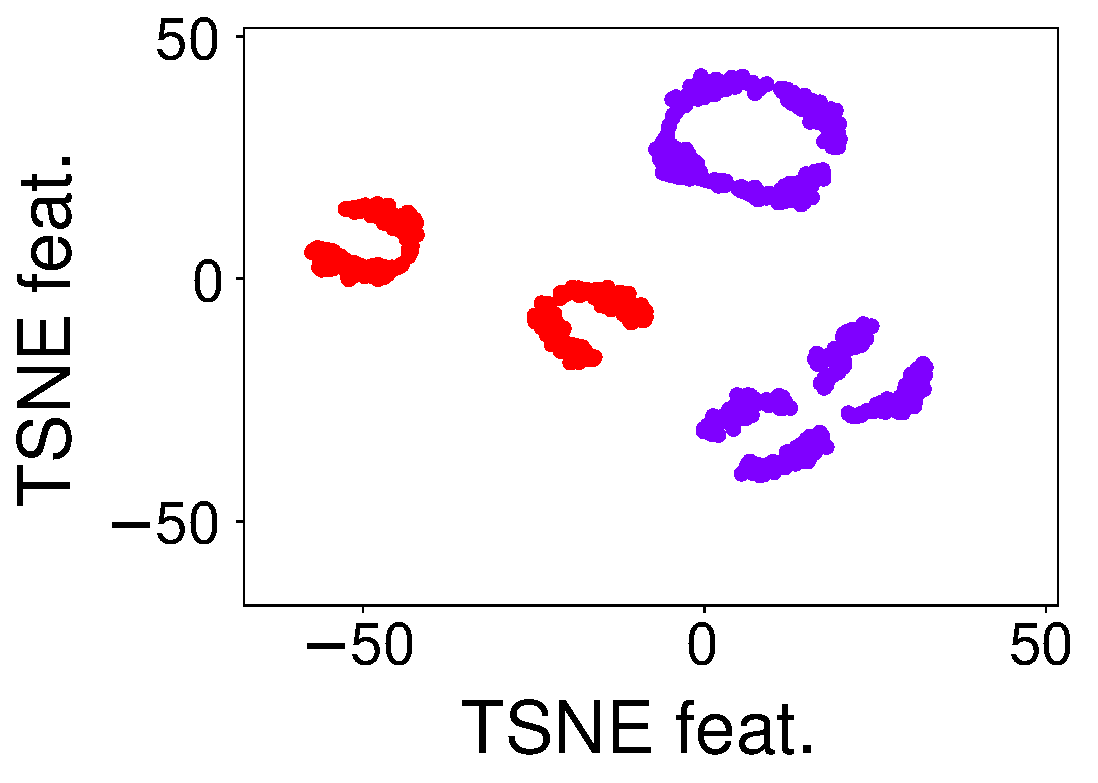
\includegraphics[scale=.15]{chapters/data-centric/unsupervised/img/cl.pdf}
        \caption{Cl\\$\quad$AMI=0.41, sil=0.41}
        \label{clustering-fig:ca3}
    \end{subfigure}
    \hfill
    \begin{subfigure}[b]{0.23\columnwidth}
        \centering
        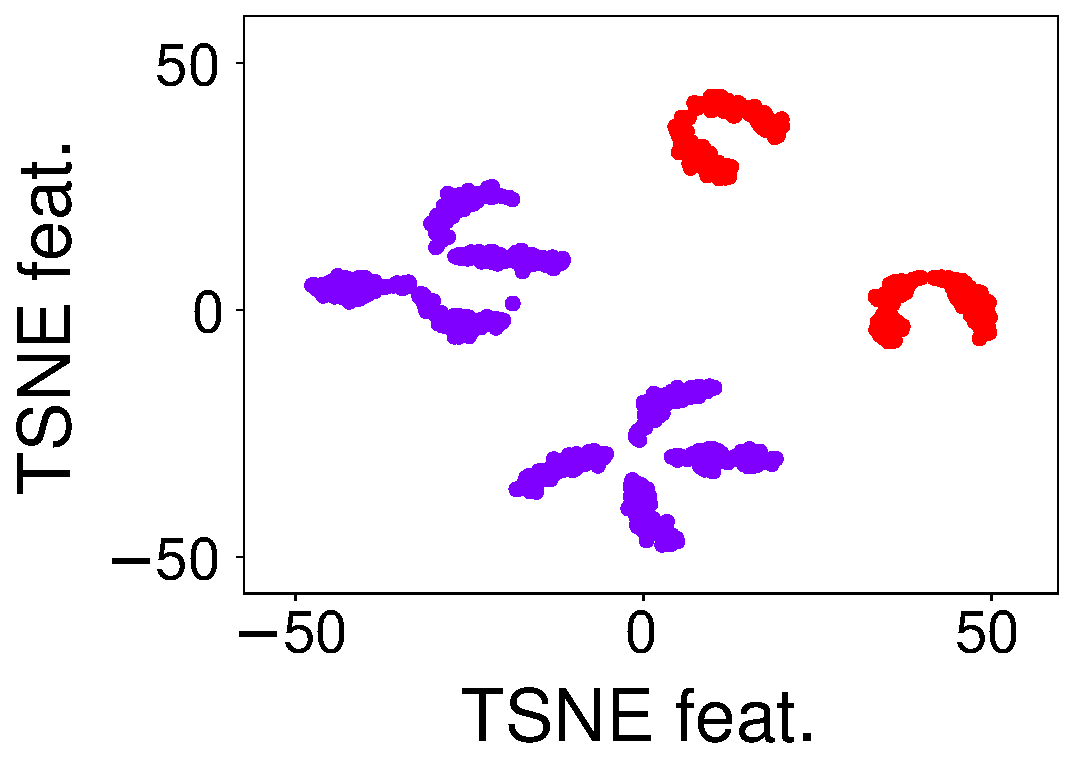
\includegraphics[scale=.15]{chapters/data-centric/unsupervised/img/ft_cl.pdf}
        \caption{FS + Cl\\$\quad$AMI=0.41, sil=0.47}
        \label{clustering-fig:ca4}
    \end{subfigure}
    \hfill
    \begin{subfigure}[b]{0.2\columnwidth}
        \centering
        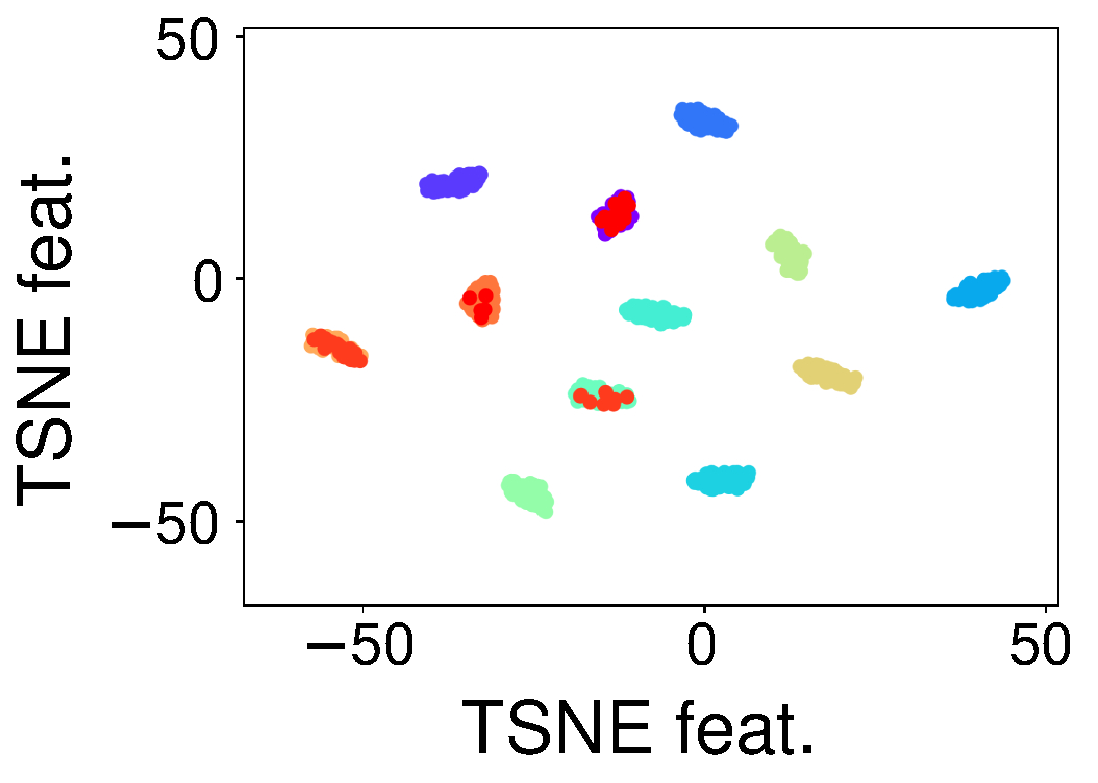
\includegraphics[scale=.15]{chapters/data-centric/unsupervised/img/ft_sc_cl.pdf}
        \caption{FS + N + Cl\\$\quad$AMI=0.9, sil=0.87}
        \label{clustering-fig:ca5}
    \end{subfigure}
    \hfill
    \begin{subfigure}[b]{0.28\columnwidth}
        \centering
        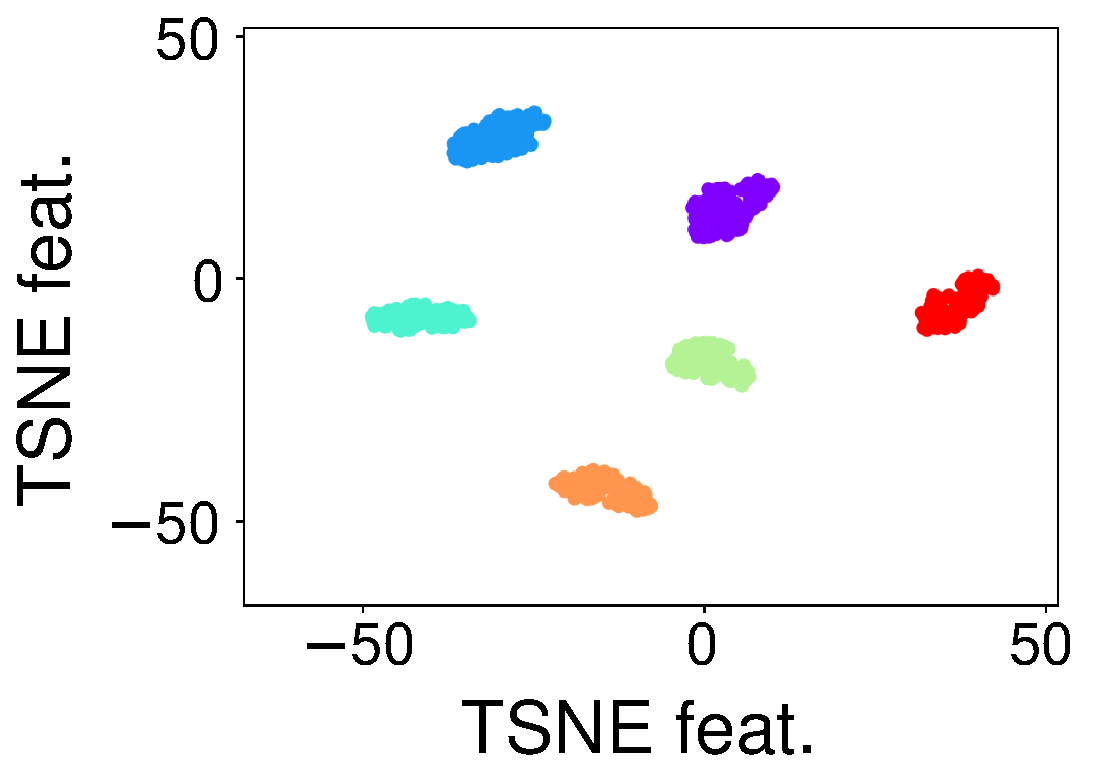
\includegraphics[scale=.15]{chapters/data-centric/unsupervised/img/ft_sc_ou_cl.pdf}
        \caption{FS + N + OR + Cl\\$\quad$AMI=1.0, sil=0.92}
        \label{clustering-fig:ca6}
    \end{subfigure}
    \caption{Approach motivation.
    \small{Feature Selection (FS) - Normalization (N) - Outlier Removal (OR) - Clustering (Cl)}}
    \label{clustering-fig:clusterings}
\end{figure}

Automated Machine Learning aids in a smart exploration of the hyperparameter search space \cite{hutter2011sequential} and lets data scientists focus on analyzing and interpreting the extracted results.
AutoML has been proven to be effective on supervised tasks where the ground truth eases the evaluation of the hyperparameters optimality   \cite{thornton2013auto,FRANCIA2023182}; yet, when it comes to unsupervised tasks, the road is not paved yet \cite{barlow1989unsupervised}.
In this chapter, we focus on the unsupervised task of (crisp) cluster analysis \cite{arthur2006k} that returns a partitioning of the original dataset based on the similarity of data items.
Cluster analysis is exploratory by nature since, given that no ground truth is available, there is no ``correct'' result \cite{no_correct_clustering,lensen2017using} and the aim for the data scientist is to uncover clues hidden in the data.
\paragraph{Challenges} The two main limitations of the AutoML approaches in the literature are (i) auto-tuning is applied to the ML step only, disregarding the pre-processing ones, and (ii) only the most-performing pipeline configuration is returned; although this is reasonable in the supervised context, it provides limited information in unsupervised one due the exploratory nature of the analysis.

\paragraph{Contributions} To overcome the previous limitations, we devise AutoClues: an \textit{end-to-end} AutoML approach that provides a \textit{dashboard} of \textit{relevant} and \textit{different} clusterings. In particular, we focus on the following contributions:
\begin{itemize}
    \item \textit{generalizing} AutoML formulation to unsupervised tasks dealing with ML pipelines;
    \item \textit{tuning} a thorough ML pipeline to discover clusterings that would have been unrevealed otherwise;
    \item \textit{diversifying} the generated clusterings to ensure that the dashboard is both high-quality and leads to different insights (i.e., disclose something new);
    \item \textit{providing} a customizable generator of synthetic datasets for benchmarking in (crisp) cluster analysis.
\end{itemize}

To let the reader appreciate the novelty of AutoClues, we rely on a synthetic 10-dimensional (10D) dataset that includes 6 natural clusters. \Cref{clustering-fig:ca3} shows the t-SNE \cite{van2008visualizing} visualization\footnote{Clusterings in more than two dimensions will be always visualized in 2D applying the t-SNE dim.reduction.}  of the clustering obtained applying AutoML4Clust \cite{Tschechlov2021}, an approach of the literature, that solely tunes the clustering step $Cl$. \Cref{clustering-fig:ca4,clustering-fig:ca5,clustering-fig:ca6} show the clusterings obtained by tuning an ML pipeline that incrementally includes feature selection ($FS$), normalization ($N$), and outlier removal ($OR$). In (b), $FS$ identifies the most relevant features; in (c), $N$ standardizes such features thus avoiding bias due to different domain ranges; in (d), $OR$ drops any data items that are not representative.
It is apparent how the tuning improves throughout the different steps, making it possible for $Cl$ to properly detect the 6 natural clusters.
To quantitatively understand the improvements, we rely on the silhouette index $sil \in [-1, 1]$ (the higher the better), an estimation of the ``goodness'' of a clustering considering solely the data itself; namely, the \textit{separability} between the clusters and their \textit{cohesion} \cite{zhu2010clustering}.
While in real-case unsupervised problems the ground truth is not available, for our synthetic example we can also measure how the returned clusters match the synthetic ones through the adjusted mutual information \cite{vinh2009information} $AMI \in [0, 1]$ (the higher the better).

\begin{figure}[t]
    \begin{subfigure}[t]{0.31\columnwidth}
        \centering
        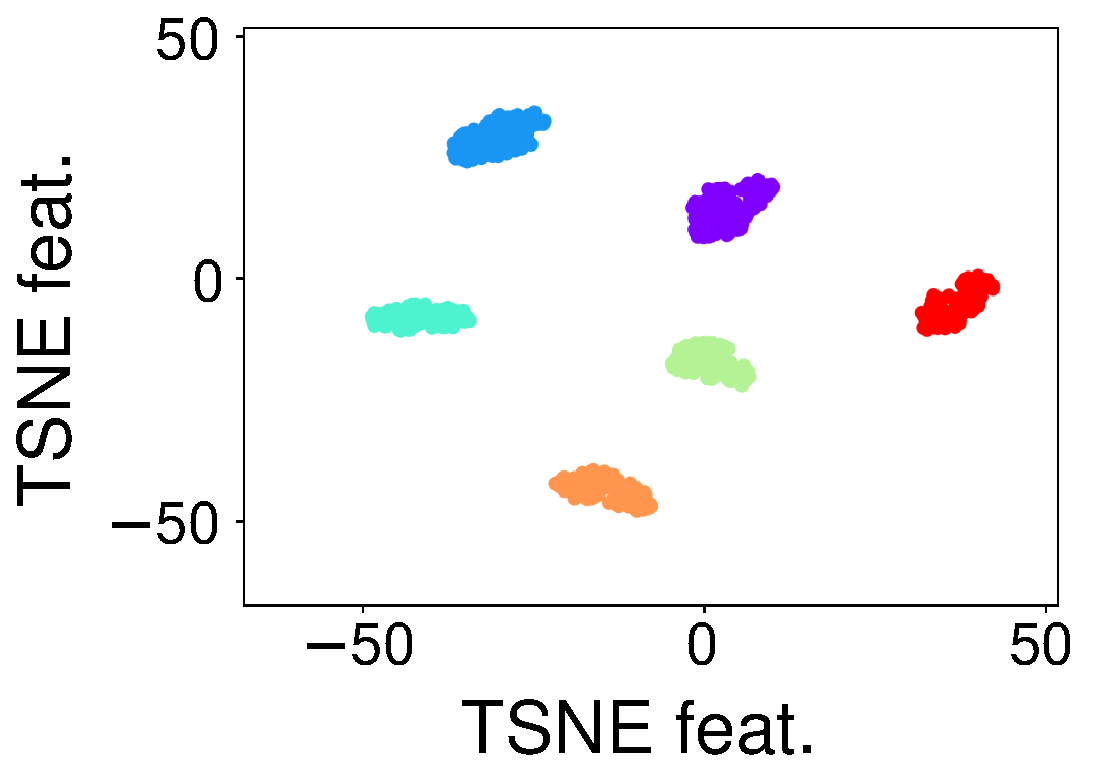
\includegraphics[scale=.15]{chapters/data-centric/unsupervised/img/ft_sc_ou_cl.pdf}
        \caption{FS + N + OR + Cl\\$\quad$AMI=1.0, sil=0.92}
        \label{clustering-fig:d1}
    \end{subfigure}
    ~~
    \begin{subfigure}[t]{0.31\columnwidth}
        \centering
        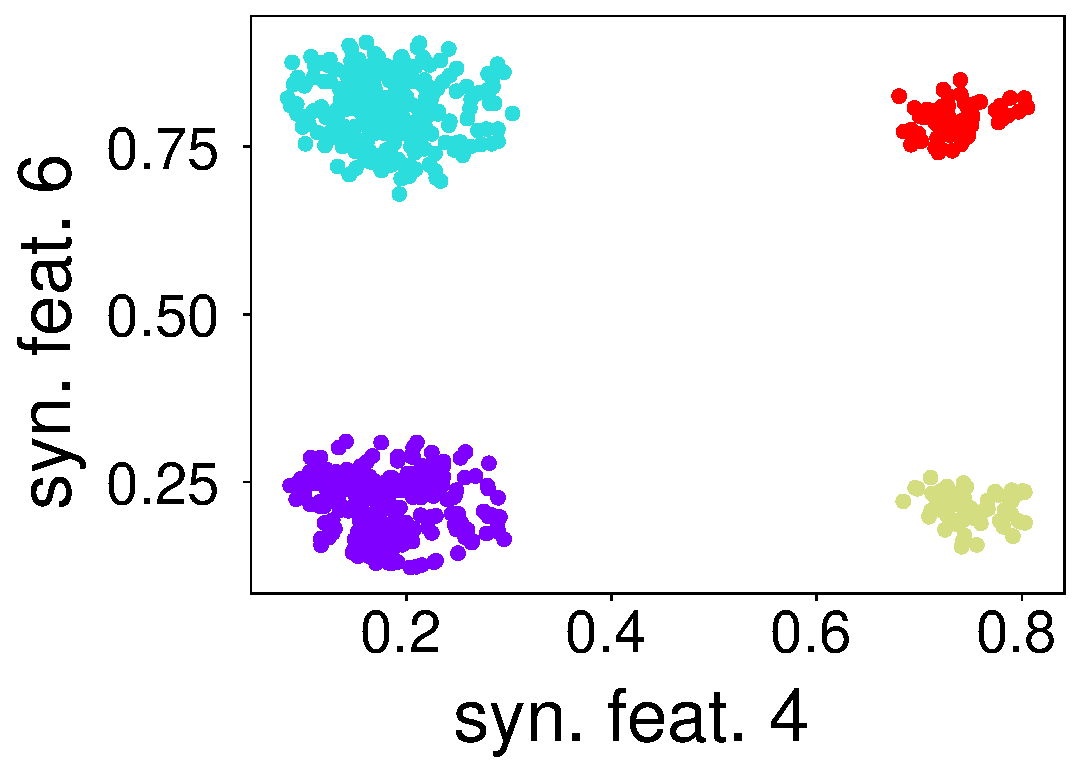
\includegraphics[scale=.15]{chapters/data-centric/unsupervised/img/dashboard_1_pred.pdf}
        \caption{FS + OR + Cl\\$\quad$AMI=0.65, sil=0.86}
        \label{clustering-fig:d3}
    \end{subfigure}
    ~
    \begin{subfigure}[t]{0.31\columnwidth}
        \centering
        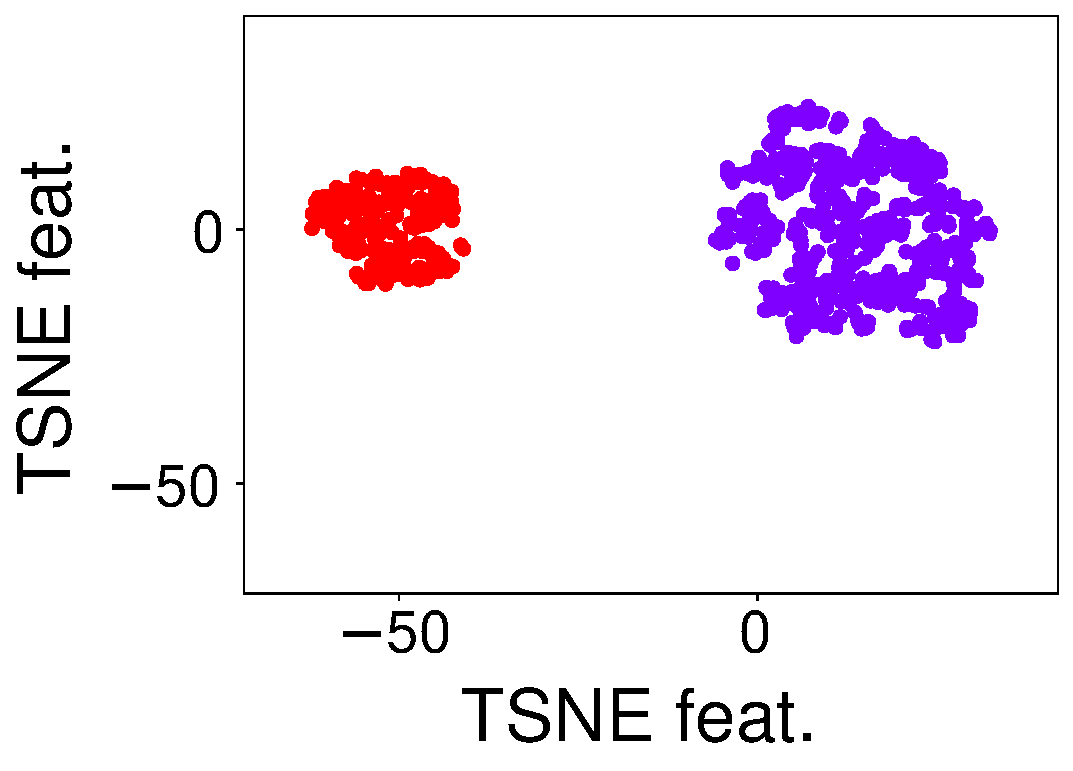
\includegraphics[scale=.15]{chapters/data-centric/unsupervised/img/dashboard_2_pred.pdf}
        \caption{FS + OR + Cl\\$\quad$AMI=0.38, sil=0.74}
        \label{clustering-fig:d2}
    \end{subfigure}
    \caption{Relevant and diverse clusterings returned by AutoClues.\\
    \small{Feature Selection (FS) - Normalization (N) - Outlier Removal (OR) - Clustering (Cl)}}
    \label{clustering-fig:dashboard}
\end{figure}

As to the limitation of returning only the most-performing pipeline configuration, \Cref{clustering-fig:dashboard} depicts an example of an AutoClues dashboard with three different facets (clustering).
Along with the expected clusters (a), the representation in (b) unveils 4 macro clusters in 2 original features, while the representation in (c) highlights a large gap of 2 main clusters.
In real-world problems, those facets may help the data scientist to understand the data by providing different interpretations of their semantics.

We organize this chapter as follows.
\Cref{clustering-sec:related} discusses the related works; \Cref{clustering-sec:autoclues} introduces the problem formulation and how AutoClues tackles it; \Cref{clustering-sec:test} illustrates the benchmark generator and dives into the empirical evaluation of the approach; finally, \Cref{clustering-sec:conclusion} draws the conclusion and future research directions.

\section{Related Works}\label{clustering-sec:related}

Although the active development of data pre-processing techniques in cluster analysis (e.g., outlier removal, feature selection), and the evidence of their benefits, there is no trace of automatic solutions that tunes a thorough ML pipeline.

Former approaches employed model-free techniques (i.e., without a model to drive the optimization) to tune the combination of number of clusters and number of features.
Evolutionary algorithms are population-based heuristics inspired by biological evolution mechanisms (e.g., reproduction, mutation) or physical phenomena (e.g., particle swarm, black holes).
The population is intended as the search space, individuals are configurations, and a mutation mechanism allows the modification of the current candidate, hence the exploration.
Recent works that follow this modus operandi (i.e., MOGA \cite{dutta2013}, MODE-cf \cite{hancer2020new}) compose the candidate with a string that encodes information about both the feature selection and the clustering.
Authors in \cite{simulate_annealing} leverage simulate annealing, an algorithm that comes from a technique involving heating and controlled cooling of material in metallurgy.
In \cite{prakash2019gravitational}, it is leveraged a gravitational search algorithm, inspired by the theory of Newtonian gravity.

Model-based techniques leverage past evaluations to fit a model and visit the most prominent configurations.
Such techniques have been proven to achieve extremely good results, specifically in the (supervised) AutoML field where a pipeline has to be instantiated with different algorithms and hyperparameters.
Authors in \cite{Tschechlov2021,poulakis2020autoclust,Liu2021} apply such techniques on cluster analysis, but do not consider any pre-processing phase.
In MALSS \cite{Kamoshida2020}, the authors apply AutoML with simple (no-clustering-oriented) pre-processing, and still for the aim of suggesting the number of clusters.
Besides, such approaches retrieve just one solution.

\section{AutoClues}\label{clustering-sec:autoclues}

\begin{figure}[t]
    \centering
    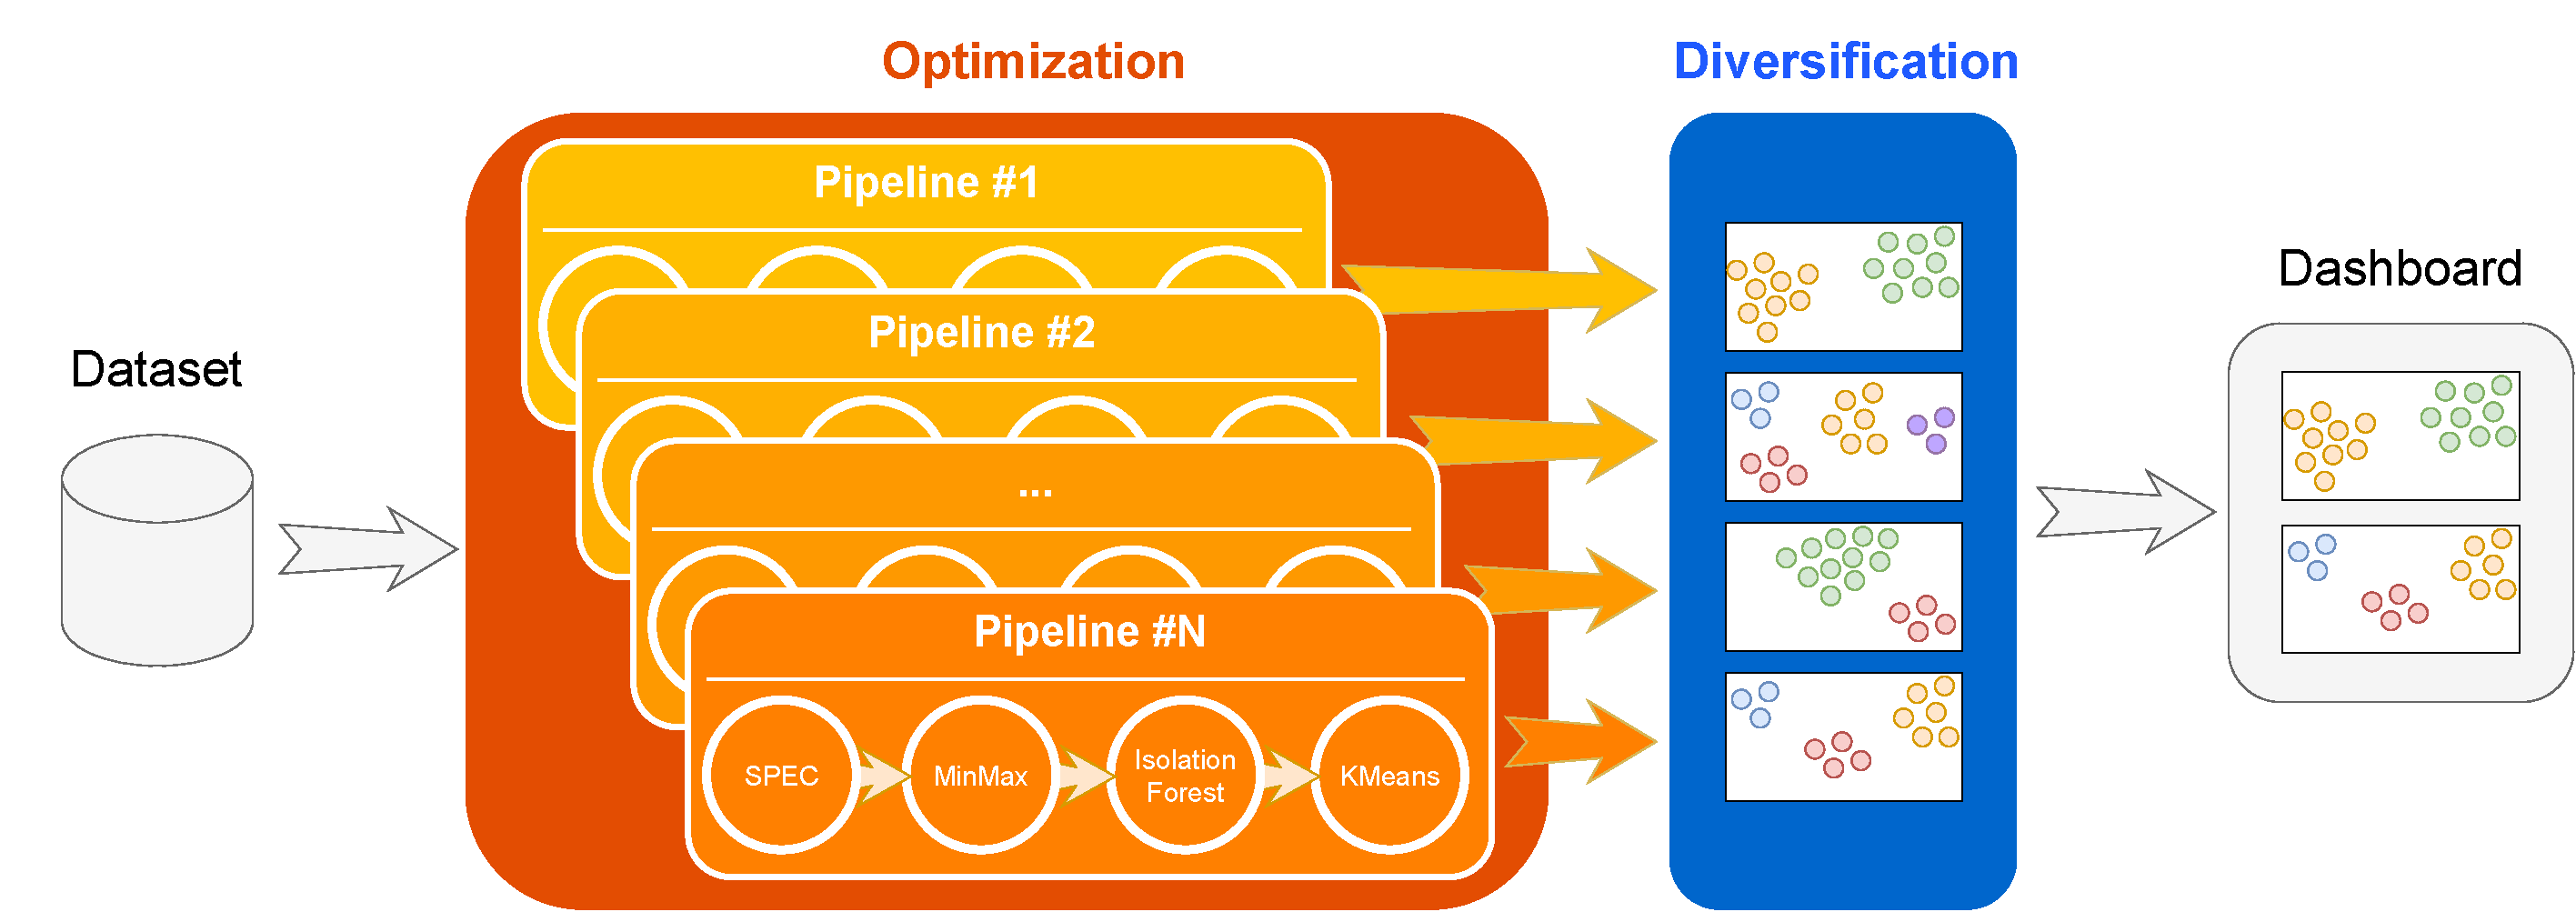
\includegraphics[scale=.33]{chapters/data-centric/unsupervised/img/approach.pdf}
    \caption{Overview of AutoClues.}
    \label{clustering-fig:overview}
\end{figure}

\Cref{clustering-fig:overview} shows an overview of the AutoClues architecture:  the optimization phase tunes the whole ML pipeline by leveraging AutoML techniques (\Cref{clustering-ssec:automl}), diversification suggests a dashboard of diverse and relevant clusterings (\Cref{clustering-ssec:diversification}).

\subsection{Optimization}
\label{clustering-ssec:automl}

In cluster analysis, we seek for the most ``correct'' pipeline.
Let us refresh the used formalization.
An ML pipeline is a sequence of pre-processing steps that shape a dataset and an ML algorithm that tackles the task---in our case, deliver a clustering.
At each step, including the final ML steps, an implementation can be picked among several alternatives---transformation for pre-processing steps, and algorithms for the ML step.
In the following, for the sake of simplicity and readability, we refer to \textit{algorithm} to a generic candidate implementation for the step at---either pre-processing or ML.

More formally, a \textit{dataset} $D$ is a collection of $|D|$ data items that is characterized by a set of features $\altmathcal{F}$ (i.e., columns).
An \textit{Algorithm} $A$ trains a model that satisfy a certain task, which nature can be either the one of pre-processing -- transforming a dataset $\altmathcal{D}$ into a new dataset $\altmathcal{D}'$ -- or the one of ML---learning how to from cluster/partition the dataset $\altmathcal{D}$.
Algorithms have a set of (possibly empty) \textit{hyperparameters} that regulates its behavior.
Each hyperparameter has a domain, and the possible algorithm configurations are represented as the Cartesian product of all the hyperparameter domains, here denoted with $\pmb{\Lambda}_A$.

A \textit{step} $S$ of the pipeline can be instantiated from several alternative algorithms; in terms of optimization search space, this can be formulated as $\Lambda_S = \Lambda_{A_1} \cup \ldots \cup \Lambda_{A_{|S|}} \cup \lambda_r$, with $\lambda_r$ a new root-hyperparameter that selects the algorithm.

A \textit{pipeline} $P$ is a sequence of steps, which search space translates to the Cartesian Product of the step spaces $\Lambda_P = \Lambda_{S_1} \times \ldots \times \Lambda_{S_{|P|}}$.
Note that we do not consider multiple possible prototypes here, so no more root hyperparameters are introduced to select the order of the steps.

A \textit{(crisp) Clustering} is a partition of the dataset into a set of (non-overlapping) clusters  $C=\{c_1, \ldots, c_{|C|}\}$ (i.e., groups of data items) by minimizing the distance of data items in the same cluster and maximizing the distance of different clusters.
Given the search space $\Lambda_P$, a dataset $\altmathcal{D}$, the optimal pipeline instance is
\begin{equation}
\label{eq:optimization}
    P_{\lambda^*} = argmin_{\lambda \in \Lambda_P} rel(P_{\lambda}(\altmathcal{D}))
\end{equation}
where $rel$ is a goodness metric\footnote{With reference to \Cref{def:loss}, a goodness metric has the opposite semantics wrt. the loss function, hence the higher the better} for the clustering $C$ obtained by partitioning the dataset through the pipeline at hand $P_{\lambda}(\altmathcal{D})$---e.g., Silhouette index \cite{sil}.


\begin{table}[!ht]
    \centering
    \begin{tabular}{lp{5cm}cc}
        \hline
        Step     & Algorithm & \#Hyper. & $|\Lambda_A|$\\\hline
        Feature selection & SPEC \cite{zhao2007spectral} & 1 & $|\altmathcal{F}|-1$\\
         & WKMeans \cite{WKMeans} & 2 & $3 \cdot (|\altmathcal{F}|-1)$\\
         & Pearson Filtering & 1 & 10\\
        Normalization     & Standardization & 0 & 1\\
        & Robust Scaling & 3 & 12\\
        & MinMax & 0 & 1\\
        Outlier Removal   & Local Outlier Factor \cite{breunig2000lof} & 1 & 3\\
        & Isolation Forest \cite{liu2012isolation} & 1 & 3\\
        %Cluster analysis  & KMeans \cite{arthur2006k} & $n \in [2.. \frac{|D|}{2}]$ \\
        Clustering  & KMeans \cite{arthur2006k} & 1 & $\sqrt{|D|}$\\
        & Agglomerative clustering  \cite{murtagh2017algorithms} & 1 & $\sqrt{|D|}$\\\hline
    \end{tabular}
    \caption{Steps and algorithms optimized by AutoClues.}
    \label{clustering-tbl:processing}
\end{table}


\paragraph{Implementation} \Cref{clustering-tbl:processing} reports the pipeline with steps, algorithms, and hyperparameters; AutoClues implementation can be found at \url{https://github.com/anonymous-pakdd-24/autoclues}.
The first step is \textit{Feature selection}.
Since cluster analysis is particularly sensitive to irrelevant features, this step aids in identifying the most informative ones.
We leverage algorithms from the spectral family (SPEC and WKMeans), techniques that demonstrated to be effective in unsupervised tasks \cite{alelyani2018feature}, and based on the Pearson correlation.
Follows, \textit{Normalization} to adjust values on different scales and ensure that all the features contribute equally to the cluster formation.
Here, the literature has a considerable consensus on the well-known techniques such as Standardization, Robust scaling, and Min-max that leverage statistical indicators; respectively: mean and standard deviation, median and quantile range, and max and min.
The last pre-processing step is \textit{Outlier Removal} for discarding any data points that are not representative of the cluster.
Local Outlier Factor \cite{breunig2000lof} measures the anomaly score of each data item based on its local density deviation compared to its neighbors and Isolation Forest \cite{liu2012isolation} isolates elements by randomly selecting a feature and a split value within its minimum and maximum values.
Finally, the \textit{Clustering} step.
Since we focus on \textit{crisp spherical} clustering algorithms, we consider KMeans \cite{arthur2006k} and Agglomerative Clustering \cite{murtagh2017algorithms} with complete linkage.
The former separates the data items into groups so that each of them has an equal variance, minimizing a criterion known as the inertia or within-cluster sum-of-squares.
The latter builds a hierarchy of clusters by merging smaller clusters into larger ones.
As to the order of steps, in \cite{giovanelli2022data}, the authors reduce the combinations of the former steps; we further constrained the order of the steps by computing several experiments and observing the impact of different alternatives.
Our implementation imports the algorithms from the Scikit-learn Python library \cite{scikit-learn}.
While the algorithms can require the assignment of additional hyperparameters (e.g., the maximum number of iterations in KMeans), we reduce the pipeline domain by considering only the most influential.

To explore promising pipelines, we leverage the SMBO implementation from the Python library HyperOpt \cite{HyperOptICML13}.
Selecting the optimal pipeline requires the relevance metric (i.e., $rel(C)$) to evaluate the goodness of the corresponding retrieved clustering.
In AutoClues, such a metric is customizable.
Well-known metrics leveraged for spherical clustering are: the silhouette index (SIL) \cite{zhu2010clustering}, contrasting the average distance to elements in the same cluster with the average distance to elements in other clusters, and the Davies-Bouldin Index (DBI) \cite{dbi}, computing the average similarity between clusters by comparing it with the size of the clusters themselves.
However, clustering metrics show a bias toward lower dimensionalities i.e., yielding higher scores when fewer features are chosen \cite{lensen2017using,hancer2020new}.
To overcome this issue, we employ t-SNE \cite{van2008visualizing} for projecting the clusterings into a latent 2D space.
Then, we compute the chosen metric in this transformed space, thereby removing the bias and enabling a fair evaluation of the clusterings across diverse feature spaces.


\subsection{Diversification}
\label{clustering-ssec:diversification}

The process of returning a set of relevant and diverse solutions -- clusterings in our case -- is known as diversification, a multi-objective optimization problem that can be formulated as follows.
Let $\altmathcal{C}$ be the set of clusterings that have been previously explored in the pipeline optimization process (\Cref{eq:optimization}), then our goal is selecting a set of $\alpha$ clusterings $\altmathcal{C}^* \subseteq \altmathcal{C}$ maximizing a \textit{score} that represents a tradeoff between finding \textit{relevance} and \textit{diversity}.
\begin{align}\label{def:score}
&\altmathcal{C}^* = argmax_{\hat{\altmathcal{C}} \subseteq \altmathcal{C}, \alpha=|\hat{\altmathcal{C}}|} score(\beta, \hat{\altmathcal{C}})\\
&score(\beta, \hat{\altmathcal{C}}) = (1-\beta)~rel(\hat{\altmathcal{C}}) + \beta~div(\hat{\altmathcal{C}})
\end{align}
where $\beta \in [0.. 1]$ is the tradeoff parameter and
\begin{align}
rel(\hat{\altmathcal{C}}) &= (|\hat{\altmathcal{C}}|-1)\sum_{C \in \hat{\altmathcal{C}}} rel(C)
\label{def:rel}
\end{align}
\begin{align}
div(\hat{\altmathcal{C}}) &= \sum_{C_i \in \hat{\altmathcal{C}}}~\sum_{C_j \in (\hat{\altmathcal{C}} \setminus C_i)} div(C_i, C_j)
\label{def:div}
\end{align}

\noindent $div(\hat{\altmathcal{C}})$ is the sum of pair-wise clustering diversity comparisons and $rel(\hat{\altmathcal{C}})$ is the sum of clustering relevance;
$rel(\hat{\altmathcal{C}})$ entails a multiplication factor $|\hat{\altmathcal{C}}|-1$ to make $rel(\hat{\altmathcal{C}})$ and $div(\hat{\altmathcal{C}})$ comparable.


\paragraph{Implementation}
Implementing diversification in cluster analysis consists of evaluating the extent to which two clusterings differ from each other.
This affects how the dashboard of returned clusterings looks like, ensuring the goal of returning different dataset facets.
It is crucial to rely on a metric that goes beyond the mere identification of shared cluster membership among different clusterings but, rather, takes into account structural interrelationships within them.

Information theory introduces the concept of Mutual Information, quantifying the degree of dependence between two variables and, more specifically, Adjusted Mutual Information (AMI) allows for chance agreement\footnote{In statistics, it serves as a baseline for assessing the significance in random variations.}---providing more robust and meaningful measures.
When applied to cluster analysis, AMI $\in [0, 1]$ considers the labels assigned to data points within clusters, assuming higher values when the clusters in one partition align with those in another.
Since we need a diversity metric, we adapt the formula as in:
$$div(C_i, C_j) = 1- AMI(C_i, C_j)$$
where $C_i, C_j$ clusterings come from different pipeline instances.

Finally, considering that the diversification problem is NP-hard, we compute it by exploiting the MMR heuristic solution \cite{vieira2011query} that selects the best-performing clustering and iteratively adds the clusterings that most diversify the outcome.

\section{Benchmark Generation and Empirical Evaluation}\label{clustering-sec:test}


\begin{table}[t]
    \centering
    \begin{tabular}{l|ccccccc|cccc}
    \hline
        \multirow{2}{*}{Dataset}& \multicolumn{7}{c|}{Characteristics} & \multicolumn{4}{c}{AutoClues Performance} \\
        & $|D|$ & $|\altmathcal{F}|$ & $|\altmathcal{C}|$ & $\sigma(D)$ & $\sigma(\altmathcal{F})$ & $SIL_N$ & $SIL_B$ & $SIL$ & $AMI$ & Score & Div. time (s) \\ \hline
         \texttt{syn1} & 2905 & 2  & 3 & 0.15  & 0.50  & 0.72 & 0.48 & 0.79 & 1.0 & 4.12 & \num{1.64e03} \\ 
        \texttt{syn2} & 264 & 5  & 3 & 0.25  & 0.20  & 0.64 & 0.4 & 0.7 & 0.83 & 4.76 & \num{1.74e02} \\ 
        \texttt{syn3} & 900 & 7  & 12 & 0.11  & 0.14  & 0.88 & 0.6 & 0.92 & 1.0 & 4.39 & \num{1.51e03} \\ 
        \texttt{syn4} & 1446 & 2  & 13 & 0.22  & 1.00  & 0.59 & 0.31 & 0.85 & 0.95 & 3.92 & \num{2.99e03} \\ 
        \texttt{syn5} & 1673 & 4  & 8 & 0.17  & 0.25  & 0.71 & 0.54 & 0.81 & 0.99 & 4.22 & \num{2.18e03} \\ 
        \texttt{syn6} & 2905 & 2  & 3 & 0.15  & 0.50  & 0.72 & 0.61 & 0.84 & 0.87 & 4.63 & \num{1.07e03} \\ 
        \texttt{syn7} & 264 & 5  & 3 & 0.25  & 0.20  & 0.64 & 0.41 & 0.72 & 0.86 & 3.78 & \num{1.67e02} \\ 
        \texttt{syn8} & 1639 & 8  & 21 & 0.13  & 0.00  & 0.87 & 0.69 & 0.91 & 1.0 & 4.45 & \num{3.13e03} \\ 
        \texttt{syn9} & 525 & 3  & 2 & 0.21  & 0.00  & 0.66 & 0.42 & 0.69 & 0.87 & 3.96 & \num{3.67e02} \\ 
        \texttt{syn10} & 1446 & 2  & 13 & 0.22  & 1.00  & 0.59 & 0.32 & 0.86 & 0.97 & 4.03 & \num{4.09e03} \\ 
        \texttt{syn11} & 4813 & 10  & 3 & 0.27  & 0.40  & 0.46 & 0.17 & 0.09 & 0.42 & 2.92 & \num{1.08e02} \\ 
        \texttt{syn12} & 2905 & 2  & 3 & 0.15  & 0.50  & 0.72 & 0.57 & 0.79 & 1.0 & 4.48 & \num{1.62e03} \\ 
        \texttt{syn13} & 264 & 5  & 3 & 0.25  & 0.20  & 0.64 & 0.4 & 0.74 & 0.89 & 4.37 & \num{2.75e02} \\ 
        \texttt{syn14} & 525 & 3  & 2 & 0.21  & 0.00  & 0.66 & 0.22 & 0.71 & 0.9 & 4.38 & \num{5.81e02} \\ 
        \texttt{syn15} & 2905 & 2  & 3 & 0.15  & 0.50  & 0.72 & 0.61 & 0.81 & 1.0 & 4.06 & \num{1.13e03} \\ 
        \texttt{syn16} & 264 & 5  & 3 & 0.25  & 0.20  & 0.64 & 0.49 & 0.7 & 0.88 & 3.45 & \num{1.84e02} \\ 
        \texttt{syn17} & 900 & 7  & 12 & 0.11  & 0.14  & 0.88 & 0.41 & 0.92 & 1.0 & 4.62 & \num{1.45e03} \\ 
        \texttt{syn18} & 525 & 3  & 2 & 0.21  & 0.00  & 0.66 & 0.3 & 0.69 & 0.84 & 4.34 & \num{2.85e02} \\ 
        \texttt{syn19} & 2905 & 2  & 3 & 0.15  & 0.50  & 0.72 & 0.53 & 0.86 & 0.87 & 4.79 & \num{1.28e03} \\ 
        \texttt{syn20} & 264 & 5 & 3 & 0.25 & 0.20 & 0.64 & 0.44 & 0.7 & 0.88 & 3.74 & \num{2.13e02} \\ \hline
    \end{tabular}
    \caption{Dataset characteristics and performance achieved by AutoClues.}
    \label{clustering-tbl:synthetic}
\end{table}

Evaluation in cluster analysis consists of assessing the approach performance in finding well-separated clusters and -- if available -- their alignment with a hypothetical ground truth.
It is crucial to test on datasets that conform with the leveraged clustering algorithms, e.g., in our case, containing crisp spherical clusters.
Yet, there is a lack of benchmarks (i.e., suites of datasets for fair comparisons) and the few available \cite{ClusteringDatasets,gagolewski2022framework,thrun2020clustering} are tailored to their specific scenarios.
This translates into approaches relying upon datasets from supervised tasks, with no guarantees on the underlying clusters' shape.

In \Cref{clustering-ssec:benchmark}, we introduce a benchmarking generator and a suite of synthetic datasets. In \Cref{clustering-ssec:effectiveness}, we leverage such a suite to assess the effectiveness and efficiency of AutoClues.
Finally, in \Cref{clustering-ssec:comparison}, we rely on real datasets to provide a comparison against other approaches in the literature.

\subsection{Benchmark Generation}
\label{clustering-ssec:benchmark}
The synthetic benchmarking generator is available via GitHub\footnote{\url{https:/github.com/anonymous-pakdd-24/clustering_benchmarking}\todo{metterlo su big e linkarlo}}.
We create datasets of $|D|$ instances, defining $|C|$ natural iper-spherical clusters in a space of $|\altmathcal{F}|$ features.
Then, we blur such clusters by posing common challenges faced by clustering algorithms.
This includes noise on instances $\sigma(D)$, such as the presence of outliers, and noise on features $\sigma(F)$, such as irrelevant, correlated, or distorted features.

To obtain datasets with different characteristics, we set boundaries for each of these dimensions and sample within them according to the Sobol sequence \cite{sobol1967distribution}, a quasi-random low-discrepancy search converging to an equi-distributed coverage.
In particular, the defined boundaries are: $|D|$ between $100$ and $5000$, $|F|$ between $2$ and $10$, $|C|$ between $2$ and $\sqrt{|D|}$, $\sigma(D)$ between $0.1$ and $0.3$, and $\sigma(F)$ between $0$ and $1$.
\Cref{clustering-tbl:synthetic} provides a suite of $20$ synthetic datasets.

Dataset complexity can be examined via the silhouette $SIL \in [0, 1]$, the higher the simpler.
$SIL_N$ measures the cohesion and separability of the natural clusters $C$ in their original feature space, while  $SIL_B$ measures the silhouette of blurred clusters (i.e. after introducing noise ($\sigma$)).
The former $SIL_N$ indicates the presence of well-separated clusters.
With the first quartile $Q1=0.64$, median $Q2=0.66$, and third quartile $Q3=0.72$, we observe that 25\% of datasets are complex already at this stage.
The latter $SIL_B$ registers significantly lower values: \texttt{syn11} emerges as an especially complex dataset with $SIL_B=0.17$ but, overall, we confirm the presence of a good distribution between more and less challenging datasets: $Q1 = 0.36$, $Q2 = 0.43$, and $Q3 = 0.55$.

\subsection{Effectiveness and Efficiency}
\label{clustering-ssec:effectiveness}


We test AutoClues on the suite of generated synthetic datasets.
For the optimization, we adopted the silhouette $SIL$ index as a relevance objective metric and a budget of $7200$ second ($2$ hours); for the diversification we set $\alpha=3$ and $\beta=0.5$, resulting in a dashboard of $3$ clusterings where relevance and diversity are weighted equally.
Tests are run on a single core of an Intel Core i7 machine at $3.20$ GHz and $64$ GB of main memory.
Given an AutoClues dashboard, \Cref{clustering-tbl:synthetic} provides the maximum $SIL\in [0, 1]$ as the cohesion of the found clusters and the maximum $AMI \in [0, 1]$ as the alignment with the natural ones. Besides, we report the dashboard score of \Cref{def:score}, summarizing the overall relevance and diversity in the dashboard, and the computation time (in seconds) spent during the diversification process. 

\subsubsection{Effectiveness}\label{sssec:effectiveness}
The achieved silhouette not only shows AutoClues' ability to find particularly well-separated clusters in 19 cases out of 20, but it also demonstrates to overcome the silhouette of natural clusters $SIL_N$. 
This is achieved through data pre-processing such as projecting natural clusters into more compact feature subsets and mitigating potential noise.
The only exception is \texttt{syn11}, a dataset already highlighted as critical for both intrinsic characteristics and noise applied. 
Besides, quartile values of $AMI$ ($Q1=0.87$, $Q2=0.9$, $Q3=1$) confirm a strong agreement between retrieved and natural clusters. 

As to the dashboard, considering the experimental setting ($\alpha=3$, $\beta=0.5$,  $rel, div \in [0, 1]$), the score is bounded in $[0, 6]$.
Notably, given the inherent trade-off relationship between \textit{rel} and \textit{div} in the context of a diversification problem, it is noteworthy that scores at the boundaries are less likely to manifest,
with values around $4$ already acknowledged as high-quality \cite{vieira2011query}.
Analogously, quartile values of the score ($Q1=4$, $Q2=4.34$, $Q3=4.47$) confirm Autoclues' ability to find relevant and diverse clusterings.

\subsubsection{Efficiency}\label{sssec:efficiency}
\Cref{clustering-tbl:synthetic} reports the computation time for diversification, when the optimization budget is set to 2 hours.
We can observe 25\% of datasets compute the dashboard in less than $Q1=\num{2.44e02}$ seconds ($4$ minutes), $50\%$ in less than $Q2=\num{1.07e03}$ seconds ($18$ minutes), and $75\%$ in less than $Q3=\num{1.56e03}$ seconds ($26$ minutes).
Besides, reducing the optimization budget leads to a decrease in diversification time, as fewer clusterings are evaluated, while the overall performance is largely maintained.

\begin{figure}[t]
    \centering
    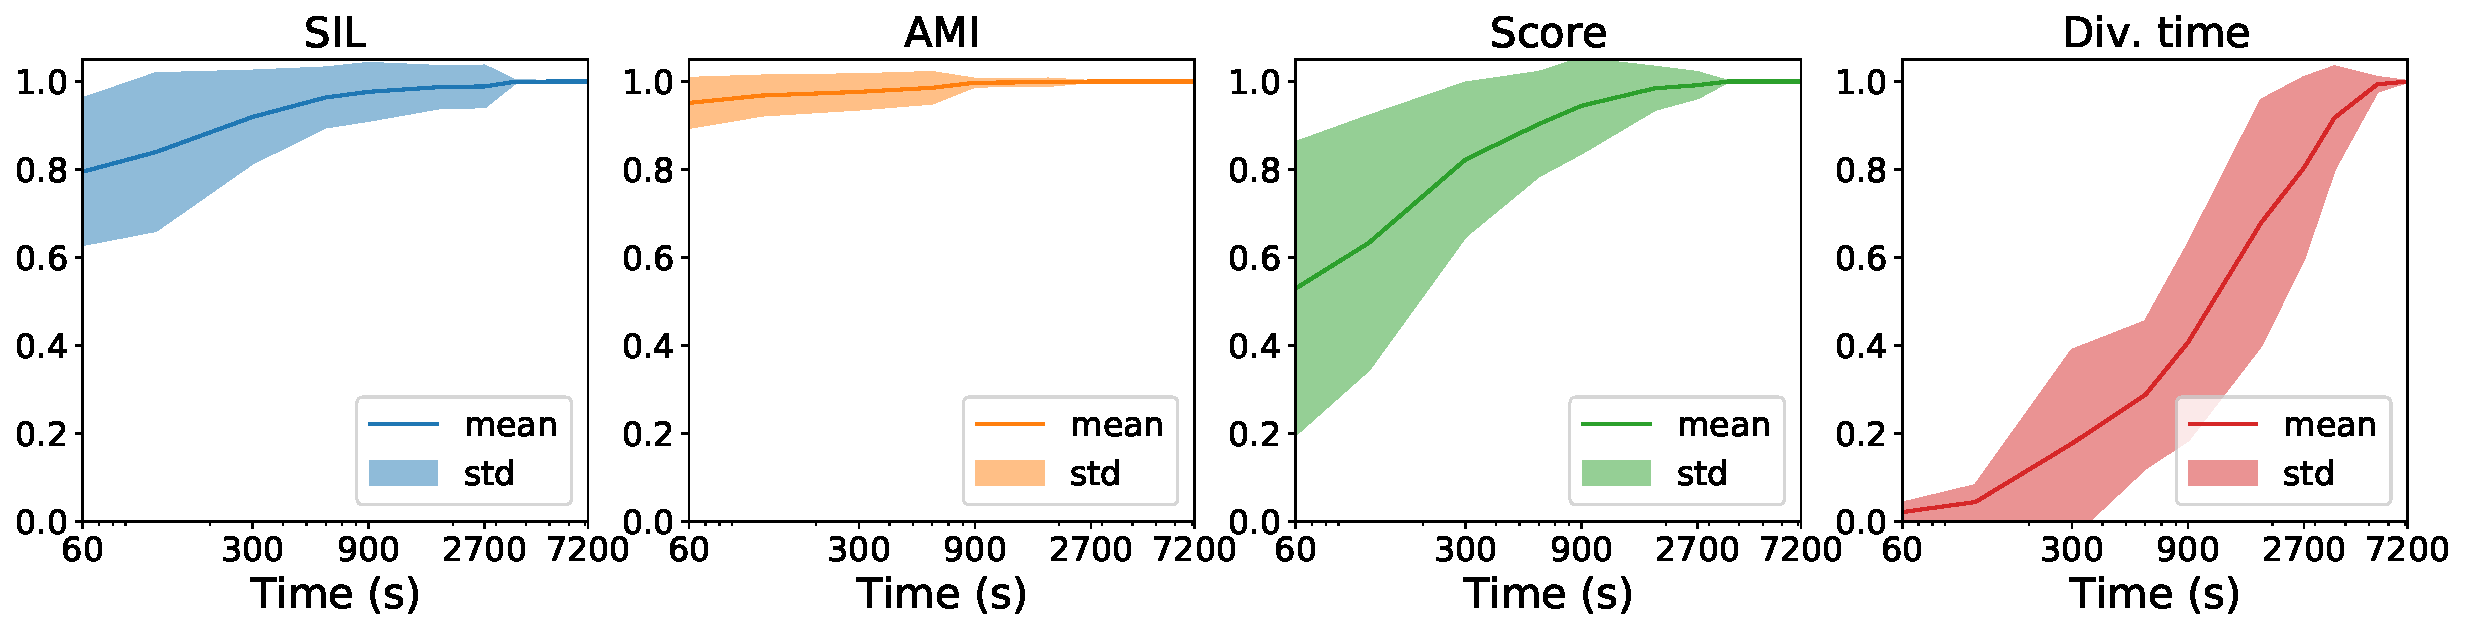
\includegraphics[scale=.3]{chapters/data-centric/unsupervised/img/all.pdf}
    \caption{AutoClues convergence through time (in log scale).}
    \label{clustering-fig:convergence}
\end{figure}

\Cref{clustering-fig:convergence} shows how AutoClues converges to the values reported in \Cref{clustering-tbl:synthetic}.
Dashboards are generated at different snapshots during the $2$-hour optimization process, and the same metrics are computed: $SIL$, $AMI$, dashboard score, and diversification time.
We summarize the information by plotting the mean and standard deviation among the whole suite, the convergence is quantified as a progress ratio relative to the final achieved performance.
Notably, the optimization time is illustrated in a logarithmic scale, which is already evidence of fast convergence.
After $60$ seconds of optimization, we have clusterings with $SIL$ and $AMI$ as good as $80\%$ and $95\%$ of the optimal and a dashboard almost $60\%$ of the final within a negligible diversification time---roughly $2\%$ of the total, $30$ seconds on average.
Within $300$ seconds of optimization, an average of $90\%$ of $SIL$, $97\%$ of $AMI$, and $75\%$ of the dashboard score are registered with a diversification cost of $10\%$---on average, $1$ minute and half.
The trends of $SIL$ and $AMI$ saturated $100\%$ right afterward, while both dashboard score and cost increase linearly until $900$ seconds of optimization, in which the dashboard achieves $90\%$ of its score within a cost of $30\%$---$5$ minutes on average.
After such a threshold, improvements in the score are not considered worth it for the computation cost.
This is due to the increasing number of available solutions that have to be evaluated during the diversification, while relevant and diverse clusterings are already present in the dashboard.

\subsection{Comparison}\label{clustering-ssec:comparison}

\begin{table}[t]
    \centering
    \resizebox{0.9\textwidth}{!}{
    \begin{tabular}{l|ccc|cccc|cc}
    \hline
        \multirow{3}{*}{Dataset} & \multicolumn{3}{c|}{Characteristics} & \multicolumn{6}{c}{Performance} \\
        & \multirow{2}{*}{$|D|$} & \multirow{2}{*}{$|\altmathcal{F}|$} & \multirow{2}{*}{$|C|$} & \multicolumn{4}{c|}{DBI $\downarrow$} & \multicolumn{2}{c}{SIL $\uparrow$} \\
        & & & & \multicolumn{1}{c}{MOGA} & \multicolumn{1}{c}{MODE-cf} & \multicolumn{1}{c}{MALSS} & \multicolumn{1}{c|}{AutoClues} & \multicolumn{1}{c}{MALSS} & \multicolumn{1}{c}{AutoClues} \\ \hline
        \texttt{blood} & 748 & 4 & 2 & - & - & 0.3 & \textbf{0} & 0.73 & \textbf{1} \\
        \texttt{breast} & 106 & 9 & 6 & - & 0.7 & 1.6 & \textbf{0.54} & 0.16 & \textbf{0.60} \\
        \texttt{ecoli} & 327 & 7 & 5 & - & 0.92 & \textbf{0.35} & 0.46 & \textbf{0.72} & 0.46 \\
        \texttt{iris} & 150 & 4 & 3 & 0.39 & 0.67 & 0.6 & \textbf{0.38} & 0.57 & \textbf{0.71} \\
        \texttt{seeds} & 210 & 7 & 3 & - & - & 0.8 & \textbf{0.4} & \textbf{0.45} & 0.37 \\
        \texttt{thyroid} & 215 & 5 & 3 & - & - & 0.64 & \textbf{0.2} & 0.6 & \textbf{0.92} \\
        \texttt{vehicle} & 846 & 18 & 4 & - & - & 0.6 & \textbf{0.15} & 0.61 & \textbf{0.72} \\
        \texttt{wine} & 178 & 13 & 3 & \textbf{0.77} & 1.22 & 1.4 & 1.01 & 0.28 & \textbf{0.38} \\ \hline
    \end{tabular}
    }
    \caption{Comparison with other approaches in the literature.}
    \label{clustering-tbl:comparison}
\end{table}


We compare AutoClues with state-of-the-art approaches in the literature against real datasets, considered as standard benchmarks.
We selected the ones that provided either the performance on classification datasets (MOGA \cite{dutta2013}, MODE-cf \cite{hancer2020new}) or code for reproducibility (MALSS \cite{Kamoshida2020}).
The former two approaches are evolutionary algorithms, and the latter is a general-purpose AutoML tool.
Note that all these approaches do not provide a dashboard of clusterings, but only the best performing one.
Thus, for a fair comparison, we set $\alpha=1$ to return the best clustering as well and we adopt as relevance the same metric used in the competing approaches.
MOGA and MODE-cf measure performance solely through the Davies–Bouldin Index ($DBI$ \cite{dbi}, the less the better),
MALLS also provides $SIL$ (the higher the better).

\Cref{clustering-tbl:comparison} shows that AutoClues outperforms the reported approaches in 6 out of 8 datasets.
According to $DBI$, MALSS achieves better performance on \texttt{seeds}, while MOGA on \texttt{wine}.
As to $SIL$, MALSS is slightly more performant in \texttt{ecoli} and \texttt{seeds}.
Yet, this is due to the fact that such approaches support the computation of non-spherical clusterings while they are not currently included in AutoClues.
Indeed, if we constraint MALSS to compute spherical clusters only, we observe a $DBI$ value of $0.79$ for \texttt{ecoli} while AutoClues achieves $0.46$ (the less the better).
As to $SIL$, MALLS achieves $0.4$ and $0.45$ for \texttt{ecoli} and \texttt{seeds} respectively; AutoClues outperforms on \texttt{ecoli} with $SIL=0.46$ and confirms the previous result on \texttt{seeds} with $SIL=0.37$.


\section{Conclusion and Future Works}\label{clustering-sec:conclusion}
We introduced AutoClues, an end-to-end cluster analysis approach that leverages AutoML techniques to provide a diverse and relevant dashboard of clusterings.
Our findings demonstrate that optimizing pre-processing significantly enhances performance, allowing AutoClues to overcome current state-of-the-art approaches. For future research, we plan to explore (i) meta-learning approaches to identify more effective pre-processing steps, (ii) integrating human feedback in the loop, and (iii) providing automatic explanations for the retrieved dashboard.

% We introduced AutoClues, an end-to-end approach for cluster analysis that explores ML pipelines through AutoML techniques and retrieves a dashboard of relevant and diverse clusterings---i.e., facets of the dataset.
% Results confirm that optimizing pre-processing boosts performance, enabling AutoClues to overcome state-of-the-art approaches. 
% AutoClues's pipeline exploration, carried out using AutoML techniques, overcomes the state-of-the-art approaches for clustering analysis since it improves the optimization of the thorough clustering pipeline. 
% As future research directions, we plan to (i) identify with meta-learning approaches which pre-processing steps are more effective to bias both optimization and diversification, (ii) include the human in the loop (e.g., learning a measure of interest by examples), and (iii) carry out an automated explanation process that describes the dashboard (i.e., which are the main insights of the facets retrieved by AutoClues).



\part{Human-centric AI}\label{part:human-centric}
% \chapter{Formalization}
\label{automl-chap:formalization}
\chapter{HAMLET: a Framework for Human-centered AutoML via Structured Argumentation}
\label{human-centric-chap:hamlet}

\begin{figure*}[t]
    \centering
    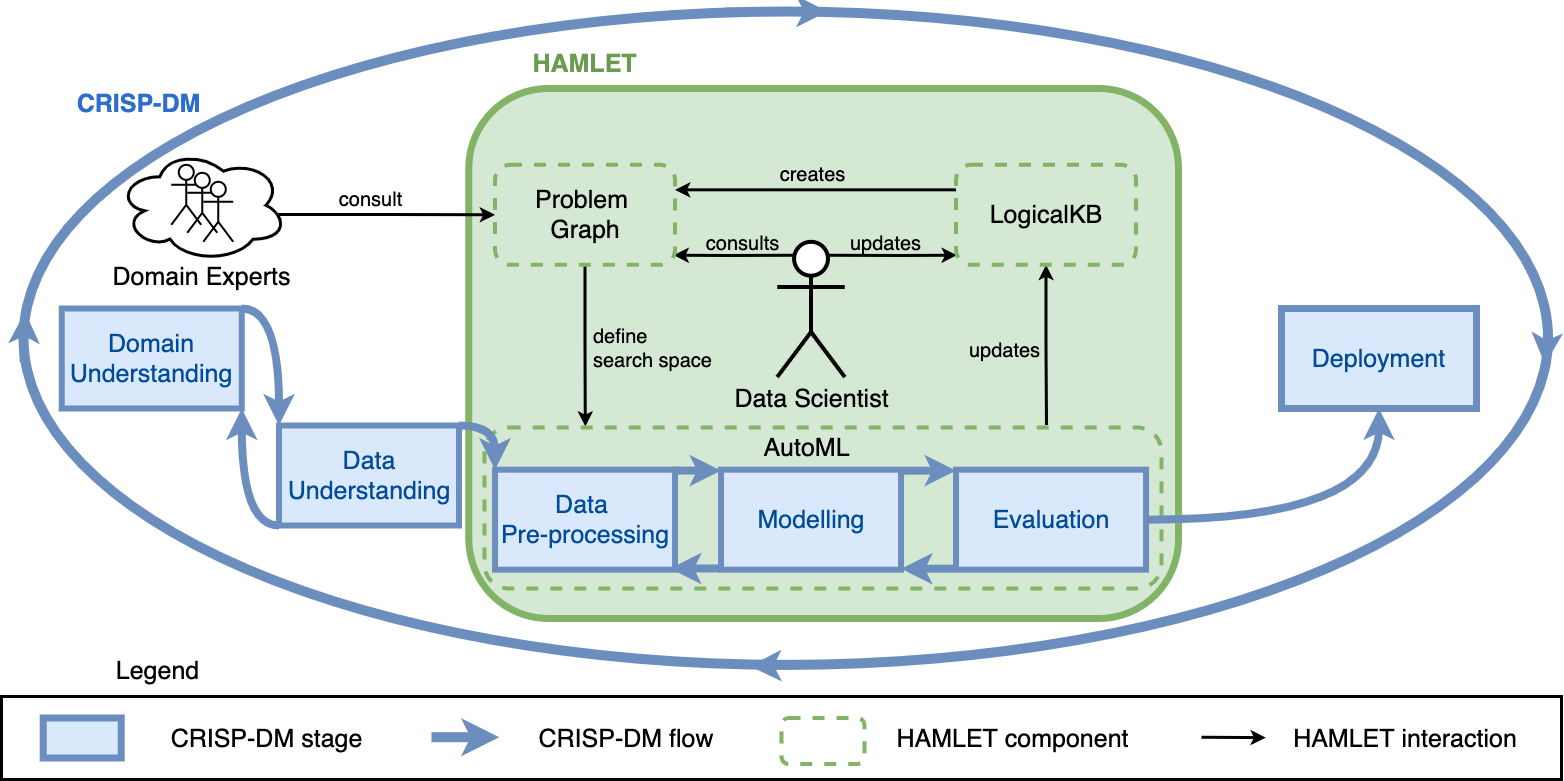
\includegraphics[scale=.25]{chapters/human-centric/hamlet/img/dymmymodel.png}
    \caption{Integrating HAMLET with the CRISP-DM process model.}
    \label{hamlet-fig:approach}
\end{figure*}

% \section{Introduction}\label{intro}
% Data platforms, integrated sets of technologies that collectively meet end-to-end data needs, work towards the automation of data management and analysis \cite{DBLP:journals/fgcs/FranciaGGLRS21}.
% Machine Learning (ML) plays a key role in such processes (e.g., to devise cost models for querying data over heterogeneous data sources \cite{multi-store} and manage data through lineage \cite{dataplat2}; many applications are well surveyed in \cite{zhou2017ml}).
% Data platforms aim at supporting end-to-end data analysis; in this scope, the Cross-Industry Standard Process for Data Mining (CRISP-DM) \cite{wirth2000crisp} is the most acknowledged standard process model---and we will take it as a reference model hencefort.
Given a Machine Learning task to solve, the data scientist collects raw data in arbitrary formats (e.g., from the data lake), builds up knowledge on both the problem and the data, translates such knowledge into \emph{constraints}, designs and trains a model, and finally deploys the solution as a new component integrated into the data platform.
Such a solution consists of a \emph{ML pipeline}.
% : a sequence of \emph{Data Pre-processing transformations} ending with an \emph{ML task}.
The data scientist instantiates the pipeline among a large set of pre-processing transformations and algorithms, which, in turn, can potentially have many \emph{hyperparameters}.
The accuracy of the deployed solution depends on finding both the best algorithms along with their hyperparameters within an exponential search space.

% Automated Machine Learning (AutoML) tools assist the data scientist in finding such an ML pipeline.
% They leverage state-of-the-art optimization approaches to smartly explore huge search spaces of solutions.
AutoML has been demonstrated to provide accurate performance, even in a limited time/iteration budget.
Yet, when setting up the search space, it is highly important for the data scientist to inject her knowledge about the problem into constraints that prevent the AutoML tool from retrieving invalid solutions (i.e., the result of those cannot be deemed correct).
However, the support for constraint/knowledge injection is limited and the AutoML tools became that complex to make it difficult for the data scientist to understand their functioning, hence losing control over the process \cite{XinWLSP21automationml}.

\paragraph{Motivation} The need for a Human-centered and explainable framework for AutoML is real \cite{gil2019towards, lee2020human, wang2019human} (or even mandatory in recent analytic scenarios where the user is interacting with mixed-reality and smart assistants \cite{DBLP:conf/dolap/FranciaGR19,DBLP:journals/is/FranciaGG22}).
It is crucial for the data scientist to augment her knowledge by learning new insights (e.g., new constraints) from the retrieved solutions.
Indeed, the data scientist requires understanding the AutoML process in order to trust the proposed solutions \cite{drozdal2020trust}.
Some works \cite{gil2019towards, lee2020human, wang2019human} prescribe the usage of a Human-centered framework for AutoML, yet they only suggest design requirements.
Alternatively, the authors in \cite{ono2020pipelineprofiler} have proposed a tool that visualizes the best and the worst solutions retrieved by an AutoML tool.
We claim that a Human-centered framework should provide the mechanisms to: (i) help the data scientist to structure her knowledge about the problem in an effective search space; and (ii) augment the knowledge initially possessed by the data scientist with the one produced by the AutoML optimization process.

\paragraph{Contributions} We introduce HAMLET (Human-centered AutoMl via Logic and argumEnTation; \Cref{hamlet-fig:approach}), a framework that enhances AutoML with Structured Argumentation to:
structure the constraints and the AutoML solutions in a Logical Knowledge Base (LogicalKB);
parse the LogicalKB into a human- and machine-readable medium called Problem Graph;
devise the AutoML search space from the Problem Graph;
and leverage the Problem Graph to allow both the data scientist and an AutoML tool to revise the current knowledge.
In this chapter, we commit to the following contributions.
\begin{enumerate}[(i)]
    \item We provide an innovative formalization of the AutoML problem, which considers ML pipelines of multiple lengths, Data Pre-processing steps and user-defined constraints.
    \item We design the formal foundation of HAMLET, supporting the injection of constraints to select ML pipelines as well as the resolution of possible arising inconsistencies.
    \item We implement a functioning prototype of HAMLET.
    \item We provide a preliminary empirical evaluation, including the overhead introduced by the argumentation process and the comparison against state-of-the-art algorithms. 
\end{enumerate}

The remainder of the paper is structured as follows. In \Cref{hamlet-sec:related}, we introduce the related works; we provide the problem formulation in \Cref{hamlet-sec:problem} and its implementation in \Cref{hamlet-sec:implementation}; finally, we provide some preliminary evaluation in \Cref{hamlet-sec:test}, and we draw the conclusions and future research directions in \Cref{hamlet-sec:conclusion}.

\section{Background and Related Works}\label{hamlet-sec:related}
HAMLET intersects two research areas, \emph{human-centric Automated Machine Learning} and \emph{Argumentation}.
In the following, we revise the corresponding related work along with the needed background.
To the best of our knowledge, no contribution lies in this intersection to provide a human-centric approach with argumentation tools.

% \subsection{Automated Machine Learning}
% AutoML tools lighten the data scientist in the overwhelming practice of finding the best ML pipeline instance (AutoML contributions mainly refer to supervised tasks).
% In the early days, only the optimization of the ML task was addressed (but no pre-preprocessing).
% Auto-Weka \cite{kotthoff2019auto} formalized the problem as ``combined algorithm selection and hyperparameter optimization'': various ML algorithms and hyperparameters are tested over a dataset to find the most performing configuration. Such optimization was successfully implemented by leveraging Bayesian optimization \cite{frazier2018tutorial}, a sequential strategy for global optimization: until a limit (budget) of iterations or time is reached, an increasingly accurate model is built on top of the previously explored configurations.

% Recently, AutoML is no longer limited to optimizing just the ML task, but it also includes Data Pre-processing \cite{Giovanelli2021DOLAP, Quemy19DOLAP}.
% In doing so, Auto-sklearn \cite{feurer2019auto} fixes the arrangement of the transformations a priori, without considering that the most performing arrangement changes according to the problem and dataset at hand.
% However, considering several arrangements translates into larger search spaces that are not easy to explore.

% Several improvements have been made to let AutoML tools explore as many configurations as possible.
% Multi-fidelity methods \cite{falkner2018bohb} (i.e., the use of several partial estimations to boost the time-consuming evaluation process) have been exploited. 
% Meta-learning leverages the previous performance of pipeline instances on a wide range of different datasets to provide several recommendations for the dataset at hand, such as promising pipeline instances (possibly acting as an alternative to Bayesian optimization) and search spaces producing good performance.
% Yet, meta-learning per se performs poorly, because it provides coarse-grained recommendations, while it is beneficial in warm-starting Bayesian optimization (i.e., the suggested pipeline instances are visited at the beginning to boost the convergence process).
% With respect to HAMLET, meta-learning per se is not expressive enough to be considered as an alternative, but can be leveraged as a support in building the LogicalKB (i.e., learning constraints that resulted effective on many similar datasets).

% We believe that the data scientist has the duty to revise and supervise the suggested solutions as well as the process producing them.
% Yet, stacking (more and more) complex mechanisms on top of each other unavoidably led to a less understandable optimization that can be hardly controlled by the data scientist (especially if without a strong computer science background).

\subsection{Human-centered AutoML Approaches}
In current state-of-the-art tools, the data scientist role in AutoML is limited to choosing the dataset to analyze, the validation technique (e.g., cross validation, hold out), and the metric to optimize (e.g., accuracy, F1 score).
AutoML researchers aim at making ML accessible to a wider audience;
this has been addressed first by improving automation and now by improving transparency, which also enables human intervention when needed.
Auto-Weka \cite{kotthoff2019auto} and Auto-Sklearn \cite{feurer2019auto} enables non-expert users to build ML models, but the ``black-box'' can be barely open.
Indeed, as advocated in \cite{drozdal2020trust}, data scientists require to understand the process to trust the proposed solutions.
This direction, named ``Human-centered AutoML'', is pursued by both researchers and companies.

As to research contributions, we found plenty of visualization wrappers.
In \cite{drozdal2020trust}, the authors raise the need of incorporating transparency into AutoML: after a session interview, they discover that -- out of all their proposed features -- model performance metrics and visualizations are the most important information to data scientists when establishing their trust in the proposed solutions.
ATMSeer \cite{wang2019atmseer} provides different multi-granularity visualizations to enable users to monitor the AutoML process and analyze the searched models.
PipelineProfiler \cite{ono2020pipelineprofiler} offers interactive visualizations of the AutoML outputs and enables the reproducibility of the results through a Jupiter notebook.
Other contributions enhance current AutoML techniques towards easier human-interactions by: (i) supporting ethic and fair constraints in Bayesian Optimization through a mathematical encoding \cite{perrone2021fair, yaghini2021human}; (ii) simplifying the usage of AutoML with symbolic annotations \cite{peng2020pyglove} and declarative languages \cite{kraska2013mlbase}; (iii) supporting fast feed-backs from AutoML (i.e., runs that are less time-consuming) by leveraging well-known mechanisms of the DBMS (e.g., lineage optimization) \cite{vartak2015supporting, xin2018accelerating}.
Recently, MILE \cite{lee2020human} has proposed to perform AutoML analysis with an end-to-end framework that reflect a DBMS (i.e., a query language + a lineage optimization).

Companies like Google and IBM are the ones most engaged in boosting the involvement of the human in the loop.
Google Vizer \cite{golovin2017google} and Google Facets\footnote{\url{https://pair-code.github.io/facets/}} are the two main visualization tools.
The former reveals details of the different hyperparameters tried in the optimization \cite{golovin2017google}, and the latter focuses on analyzing the output and recognizes biased AI (e.g., ML models that discriminate on sensible attributes such as gender).
As to IBM, AutoAI \cite{wang2020autoai} and AutoDS \cite{wang2021autods} are the tools developed within the MIT-IBM Watson AI Lab.
Specifically, the former enables non-technical users to define and customize their business goals as constraints. 
The latter assists the data scientist team throughout the CRISP-DM process (e.g., in data collection and pipeline design \cite{muller2019data, wang2021autods} and in the augmentation of the DS's knowledge about the dataset features \cite{drozdal2020trust}).

Overall, several studies have been made to understand the proper design of a Human-centered AutoML tool.
In \cite{pfisterer2019towards}, the authors overview the main AutoML issues; while in \cite{khuat2022roles} authors suggest improvements towards the Human-centered shift.
In \cite{gil2019towards, XinWLSP21automationml, crisan2021fits}, interviews with data scientists are conducted to reveal their perception of AutoML as well as their needs and expectations in the next-generation tools.
The main insight is that the future of data science work will be a collaboration between humans and AI systems, in which both automation and human expertise are indispensable \cite{wang2019human}.
To this end, AutoML should focus on: simplicity, reproducibility, and reliability \cite{XinWLSP21automationml, crisan2021fits}.

While the above-mentioned papers mainly focus on visualization, HAMLET brings the data scientist in the loop by allowing her to inject knowledge in the form of constraints, optimizing and learning new constraints through AutoML, and managing such constraints and conflicts through Argumentation.

\subsection{Logic and Argumentation}\label{logic}
Logic is defined as the abstract study of statements, sentences and deductive arguments \cite{Paulson2018logichistory}.
From its birth, it has been developed and improved widely, now including a variety of formalisms and technologies.

Argumentation is a well-known formal tool for handling conflicting information (e.g., opinions and empirical data).
In Abstract Argumentation \cite{Dung1995abstractArg}, a scenario (e.g., a legal case) can be represented by a directed graph.
Each node represents an argument, and each edge denotes an attack by one argument on another. Each argument is regarded as atomic. There is no internal structure to an argument. Also, there is no specification of what is an argument or an attack. A graph can then be analyzed to determine which arguments are acceptable according to some general criteria (i.e., semantics) \cite{baroniCG11semantics}.

A way to link Abstract Argumentation and logical formalisms has been advanced in the field of Structured Argumentation \cite{BesnardGHMPST14structured}, where we assume a formal logical language for representing knowledge (i.e., a LogicalKB) and for specifying how arguments and conflicts (i.e., attacks) can be derived from that knowledge. 
In the structured approach, the premises and claims of the argument are made explicit, and the relationship between them is formally defined through rules internal to the formalism.
We can build the notion of attack as a binary relation over structured arguments that denotes when one argument is in conflict with another (e.g., contradictory claims or premises).
One of the main frameworks for Structured Argumentation is ASPIC\textsuperscript{+}\cite{Modgil2014aspic+}.
In this formalism, arguments are built with two kinds of inference rules: strict rules, whose premises guarantee their conclusion, and defeasible rules, whose premises only create a presumption in favor of their conclusion.
Then conflicts between arguments can arise from both inconsistencies in the LogicalKB and the defeasibility of the reasoning steps in an argument (i.e., a defeasible rule used in reaching a certain conclusion from a set of premises can also be attacked).

Once defined the right logical language for encoding the data scientist and AutoML knowledge, a Structured Argumentation model (e.g., an ASPIC\textsuperscript{+} instance \cite{arg2p-jlc}) can support HAMLET with the formal machinery to build an Argumentation framework upon the data, while Abstract Argumentation would dispense the evaluation tools.

\section{Problem Formulation}\label{hamlet-sec:problem}

\Cref{hamlet-fig:approach} illustrates the overview of HAMLET.
When addressing end-to-end data analysis, a data scientist usually follows a process model such as CRISP-DM.
The data scientist starts by collecting raw data in an arbitrary format.
Then, domain understanding is conducted.
The data scientist works in close cooperation with domain experts and enlists \emph{domain-related constraints} (i.e., intrinsic of the problem).
Follows data understanding, devoted to data analysis, and to extract \emph{data-related constraints} (e.g., defined by the data format).
Domain and data understanding might be repeated many times until the data scientist is satisfied by the acquired knowledge.
Once confident, the data scientist investigates different solutions throughout data pre-processing, modelling, and evaluation.
Data pre-processing and modelling are conducted to effectively build the solution, while evaluation offers a way to measure its performance.
Such a solution consists of a ML pipeline: a sequence of pre-processing steps ending with an ML algorithm that tackles the task.
The data scientist instantiates different pipelines among a large set of transformations and algorithms; the performance are affected by both their implementation and some exposed hyperparameters.
While seeking the best performing and valid solution, the data scientist should consider the already known constraints -- domain- and data-related -- and the ones she discovers during data pre-processing and modelling, respectively: \emph{transformation-} and \emph{algorithm-related constraints} (e.g., due to the intrinsic semantic of transformations and algorithms at hand).
Finally, the process concludes with the deployment of the solution.

HAMLET intersects CRISP-DM, allowing the data scientist to inject and augment her knowledge while automatizing the exploration towards the solution (i.e., instantiate the best ML pipeline). 
We now dig the foundation of HAMLET by incrementally introducing the concepts necessary to move from AutoML to Logic and Argumentation.
% To support the reader, we summarize the main notation in \Cref{hamlet-tbl:symbols}.

\begin{table}[t]
    \centering
    \footnotesize
    \caption{Main symbols used in the formalization.}
    \begin{tabular}{cl}
        \toprule
        \textbf{Symbol} & \textbf{Meaning} \\
        \midrule
        $A$ & Algorithm \\
        $h$ & Algorithm hyperparameter \\
        $S$ & Step \\
        $P$ & Pipeline \\
        $\lambda_*$ & Instance of * \\
        $\Lambda_*$ & Domain of * \\
        $\Lambda$ & Search space \\
        \bottomrule
    \end{tabular}
    \label{hamlet-tbl:symbols}
\end{table}

\subsection{AutoML Formalization}
We provide a novel formalization necessary to move from single algorithms to the optimal pipeline.
For the sake of clarity, we refer to a Classification task, but the formalization also holds for supervised ML tasks in general. % regression tasks.

\begin{definition}[Dataset]
A \emph{dataset} $X$ is a matrix where data items (i.e., rows) are characterized by features (i.e., columns).
\end{definition}

\begin{definition}[Algorithm]
An \emph{algorithm} $A$ is a function that transforms an input dataset $X'$ into a new dataset $X''$.
The algorithm exposes a (possibly empty) set $H$ of \emph{hyperparameters}.
Each hyperparameter $h \in H$ has a \emph{domain} $\Lambda_h$.
We call the \emph{algorithm domain} $\Lambda_A$ the Cartesian product of all hyperparameter domains (i.e., $\Lambda_A = \Lambda_{h_1} \times \ldots \times \Lambda_{h_{|H|}}$).
We call \emph{algorithm instance} $\lambda_A \in \Lambda_A$ an algorithm whose hyperparameters have been assigned with values from their respective domains.
\end{definition}

A Classification algorithm returns a vector (i.e., a matrix with a single column) of labels $Y$ out of the input dataset $X'$.

\begin{definition}[Step]
A \emph{step} $S$ is a set of alternative algorithms with the same goal.
The \emph{step domain} is defined as a disjoint union of the algorithm domains $\Lambda_S = \Lambda_{A_1} \cupdot \ldots \cupdot \Lambda_{A_{|S|}}$.
\end{definition}

Where $\cupdot$ combines the domains of the given algorithms, while retaining the original domain membership (i.e., it is possible to refer to the domain of each algorithm included in a step).

We identify two types of steps: Data Pre-preprocessing steps (e.g., Discretization, Normalization) shape the dataset for the last mandatory step, which fulfill the task---Classification in this case.

\begin{example}[Algorithm and step]
Examples of steps are Normalization ($\altmathcal{N}$), Discretization ($\altmathcal{D}$), and Classification ($\altmathcal{C}l$). 
An algorithm for Classification is Decision Tree  ($\altmathcal{D}t$) \cite{DBLP:books/wa/BreimanFOS84},
examples of hyperparameters for $\altmathcal{D}t$ are its maximum $\textup{depth}$ $(\mathbb{N}^+)$ and the minimum $\textup{samples split}$ $(\mathbb{N}^+)$ required to split a node; hence $\Lambda_{\altmathcal{D}t} = \mathbb{N}^+ \times \mathbb{N}^+$.
An example of algorithm instance is $\lambda_{\altmathcal{D}t}= \{ \textup{depth}=3,\textup{samples\_split}=10 \}$.
\end{example}

\begin{definition}[Pipeline]
Given a (possibly empty) set of Pre-processing steps $\altmathcal{S} = \{S_1,\ldots, S_{|\altmathcal{S}|}\}$ and a Classification algorithm $A$ from the Classification step, a \emph{pipeline} $P$ is a sequence that concatenates steps from $\altmathcal{S}$ and $A$.
The domain of a pipeline is $\Lambda_P = \Lambda_{S_1} \times \ldots \times \Lambda_{S_{|\altmathcal{S}|}} \times \Lambda_A$.
We call \emph{pipeline instance} $\lambda_P$ a sequence of algorithm instances $\lambda_P = \langle \lambda_{A_1}, \ldots, \lambda_{A_{|P|}} \rangle$ such that $\lambda_P \in \Lambda_P$.
\end{definition}

\begin{example}[Pipeline and pipeline instance]
Given the pre-processing steps Normalization ($\altmathcal{N}$) and Discretization ($\altmathcal{D}$), the possible pipelines for the DecisionTree ($\altmathcal{D}t$) are:
\begin{align*}
    P_1 &= \langle \altmathcal{D}t \rangle &
    P_2 &= \langle \altmathcal{D}, \altmathcal{D}t \rangle & 
    P_4 &= \langle \altmathcal{D}, \altmathcal{N}, \altmathcal{D}t \rangle \\
    &&
    P_3 &= \langle \altmathcal{N}, \altmathcal{D}t \rangle & P_5 &= \langle \altmathcal{N}, \altmathcal{D}, \altmathcal{D}t \rangle
\end{align*}
Given \textup{Binarizer} ($\altmathcal{B}$) and  \textup{KBinsDiscretizer} ($\altmathcal{K}b$) as algorithms of Discretization ($\altmathcal{D}$), and \textup{MinMaxScaler} ($\altmathcal{M}m$) and \textup{StandardScaler} ($\altmathcal{S}s$) and  as algorithms of Normalization ($\altmathcal{N}$), we provide examples of instances of $P_2$ and $P_4$:
\begin{align*}
    \lambda_{P_2} &= \langle \lambda_{\altmathcal{B}},~ \lambda_{\altmathcal{D}t} \rangle, &\lambda_{P_4} &= \langle \lambda_{\altmathcal{K}b},~ \lambda_{\altmathcal{M}m},~ \lambda_{\altmathcal{D}t} \rangle \\
    \lambda_{\altmathcal{B}}&=\{ \textup{thr}=5.5 \}, &\lambda_{\altmathcal{K}b}&=\{ \textup{n\_bins}=3, \ldots \}\\
    \lambda_{\altmathcal{M}m}&=\{ \varnothing \}, &\lambda_{\altmathcal{D}t}&= \{ \textup{depth}=3,\ldots\}
\end{align*}
\Cref{hamlet-fig:space} depicts the pipeline domain $\Lambda_{P_4}$ and the pipeline instance $\lambda_{P_4}$.
\label{ex:pipelineinstance}
\end{example}

Depending the on the involved algorithms, their order and hyperparameters, the search space -- out of which the best pipeline instance is select -- is defined as follows.
While, its extraction is later discussed in \Cref{spacealgorithm}.

\begin{definition}[Search space]
The \emph{search space} $\Lambda$ is the Cartesian product of the domain of the Classification step and the disjoint union of the all partial permutations of the pre-preprocessing steps domains.
\end{definition}

AutoML optimizes the exploration of such space.
However, it is not only about algorithms and hyperparameters but also about constraints.

\begin{definition}[Constraint]\label{constraints}
A \emph{constraint} $C \subseteq \Lambda$ is a region of search space that is either \emph{mandatory} or \emph{forbidden}.
Given a pipeline instance $\lambda_P \in \Lambda_P \subseteq \Lambda$
\begin{itemize}
    \item a mandatory constraint $C$ is fulfilled if  $\lambda_P \in C$;
    \item a forbidden constraint $C$ is fulfilled if  $\lambda_P \notin C$.
\end{itemize}
\end{definition}

\begin{figure}
    \centering
    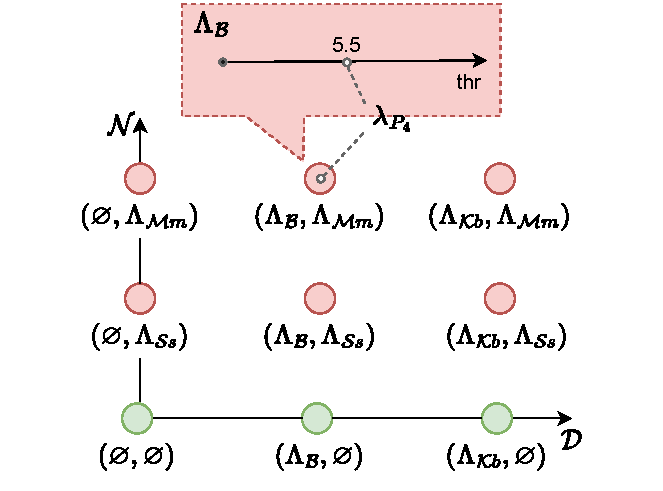
\includegraphics[scale=.75]{chapters/human-centric/hamlet/img/toy_example_ss.pdf}
    \caption{Examples of the pipeline domain $\Lambda_{P_4}$ and pipeline instance $\lambda_{P_4}$, for the sake of visualization we omit the third dimension representing the domain of the Decision Tree. Green (or red) circles represent valid (or invalid) sub-regions of the search space; Normalization is not allowed in the pipeline. The rectangle represents a zoom in the domain of the Binarizer algorithm.}
    \label{hamlet-fig:space}
\end{figure}


\begin{example}[Constraint]
Given the Normalization step ($\altmathcal{N}$) and Decision Tree ($\altmathcal{D}t$) as a Classification algorithm, an example of algorithm-related constraint is ``forbid $\altmathcal{N}$ in pipelines with $\altmathcal{D}t$''.
This discards all the pipelines containing both Normalization and Decision Tree.
\Cref{hamlet-fig:space} depicts the effects of the constraint on the pipeline domain $\Lambda_{P_4}$.
\label{ex:constraints}
\end{example}

Considering all the constraint combinations is overwhelming and, additionally, \emph{conflicts} might occur; for instance in the case of ethical \cite{boston-house} and legal fields that easily inject conflicting constraints into the search space.

\begin{definition}[Constrained pipelines optimization]
Given a search space $\Lambda$ and a set of constraints $\altmathcal{C}$, finding the best pipeline instance $\hat{\lambda}_P$ is defined as $\hat{\lambda}_P = argmax_{\lambda_P \in \Lambda_P} metric(\lambda_P)$, where $metric(\lambda_P)$ is the function evaluating the goodness of $\lambda_P$ and the explored pipelines fulfill the constraints in $\altmathcal{C}$.
\end{definition}

\subsection{Argumentation Formalization}

AutoML is not explainable, hence it does not provide the data scientist with feedbacks that would help her to augment the knowledge about the problem.
It is necessary to represent both (i) the data scientist knowledge about the problem and (ii) the outcome of the AutoML tool in a uniform human-readable medium.
The former helps to drive the optimization process,
the later augments the knowledge about the problem by learning from the explored configurations of pipeline instances---deriving new constraints that increase the data scientist awareness.
We leverage Logic as the key element in defining a common structure (i.e., a uniformed human- and machine-readable medium) on which the knowledge of both the data scientist and the AutoML tool can be combined fruitfully.
In a way, our approach follows the steps of the well known logical based expert systems, of which it is possible to find a great number of successful examples \cite{tan17es}.
Logic provides the tools to cope with one of the distinctive features of the knowledge we want to deal with: inconsistency. Indeed, the ML process is the product of possible attempts, validated or refuted by a consequent evaluation. Hence, the mechanism used to encode the knowledge is required to manage this constant revision process.
This is the role of Argumentation---one of the main approaches for dealing with inconsistent knowledge and defeasible reasoning. 

\begin{definition}[Argumentation Theory]\label{system}
An Argumentation theory is a tuple AS=$\langle L, R \rangle$ with:
\begin{itemize}
    \item $L$ an Argumentation language;
    \item $R$ the set of defeasible rules in the form $r : \phi_0,\ldots, \phi_n \Rightarrow \phi$, where $\phi_0,\ldots, \phi_n,\phi$ are well-formed formulae in the $L$ language and $r$ is the identifier of the rule; we call $\phi_0,\ldots, \phi_n$ the premises of the rule, and $\phi$ its conclusion.
    Rules with no premises are allowed (i.e. $r : \Rightarrow \phi$).
\end{itemize}
\end{definition}

The set of rules $R$ in the theory is used to define how elements from the language are combined together.
In the following two definitions, we specialize $L$ into the language $L_{ML}$ expressing all the basic elements of an AutoML problem and $R$ into a Logical Knowledge Base written in the language $L_{ML}$.

\begin{definition}[AutoML language]
Given an argumentation language $L$, we define the \emph{AutoML language} $L_{ML}$ as $L \cup W$, with $W$ the following set of predicates\footnote{For the sake of conciseness, when writing statements of the AutoML language, the letters $S$ (and $A$) refer to the name of the step (and algorithm)}:
\begin{itemize}
    \item step($S$) with $S \in L$, representing a step $S$ in the pipeline;
    \item algorithm($S$, $A$) with $S, A \in L$, representing an algorithm $A$ for the step $S$;
    \item hyperparameter($A$, $h$, $t$) with $A, h, t \in L$, representing an hyperparameter $h$ for the algorithm $A$ of type $t$ (e.g., numerical, categorical);
    \item domain($A$, $h$, $\Lambda_h$) with $A, h, \Lambda_h \in L$, representing an hyperparameter $h$ for the algorithm $A$ with domain $\Lambda_h$;
    \item pipeline($\langle S_1, \ldots, S_n \rangle$, $A$) with $S_1, \ldots, S_n, A \in L$, representing a pipeline consisting of the sequence of steps $\langle S_1, \ldots, S_n \rangle$ and the Classification algorithm $A$;
    \item mandatory($\langle S_1, \ldots, S_n \rangle$, $Z$) with $S_1, \ldots, S_n, Z \in L$, representing a constraint imposing the steps $\langle S_1, \ldots, S_n \rangle$ on the pipelines with algorithm $A$ ($Z = A$) or on all the Classification pipelines ($Z = \altmathcal{C}l$);
    \item forbidden($\langle S_1, \ldots, S_n \rangle$, $Z$) with $S_1, \ldots, S_n, Z \in L$, representing a constraint forbidding the steps $\langle S_1, \ldots, S_n \rangle$ on the pipelines with algorithm $A$ ($Z = A$) or on all the Classification pipelines ($Z = \altmathcal{C}l$);
    \item mandatory\_order($\langle S_1, \ldots, S_n \rangle$, $Z$) with $S_1, \ldots, S_n, Z \in L$, representing a constraint imposing the sequence of steps $\langle S_1, \ldots, S_n \rangle$ on the pipelines with algorithm $A$ ($Z = A$) or on all the Classification pipelines ($Z = \altmathcal{C}l$).
\end{itemize}
\end{definition}

\begin{definition}[Logical Knowledge Base]
Given the language $L_{ML}$, we call Logical Knowledge Base (LogicalKB) the set of rules for a given AutoML problem.
\end{definition}


In other words, the data scientist leverages an intuitive logical language (i.e., $L_{ML}$), and enlists the constraints one-by-one (i.e., in the LogicalKB).
In our vision, the LogicalKB consists of (i) a set rules specified by the data scientist and a (ii) set of common rules that enable the automatic derivation of pipelines and constraints.
Besides, the data scientist community could create a shared LogicalKB derived from the available literature and similar real-case problems.

\begin{example}[Logical Knowledge Base]\label{ex:kb}
We focus on Discretization ($\altmathcal{D}$),  Normalization ($\altmathcal{N}$) and Classification ($\altmathcal{C}l$) steps, and, for brevity, only define the Classification algorithms: Decision Tree ($\altmathcal{D}t$) and K-Nearest Neighbors ($\altmathcal{K}nn$).
\begin{lstlisting}[mathescape=true]
# define Discretization step
s1 : $\Rightarrow$ step($\altmathcal{D}$).
# define Normalization step
s2 : $\Rightarrow$ step($\altmathcal{N}$).
# define Classification step
s3 : $\Rightarrow$ step($\altmathcal{C}l$).
# DT is a Classification algorithm
a1 : $\Rightarrow$ algorithm($\altmathcal{C}l$, $\altmathcal{D}t$).
# Knn is a Classification algorithm
a2 : $\Rightarrow$ algorithm($\altmathcal{C}l$, $\altmathcal{K}nn$).
# Forbid Normalization when using DT
c1 : $\Rightarrow$ forbidden($\langle\altmathcal{N}\rangle$, $\altmathcal{D}t$).
\end{lstlisting}
\noindent \texttt{s1}, \texttt{s2}, and \texttt{s3} represent the steps; \texttt{a1} and \texttt{a2} represent the algorithms; finally, \texttt{c1} represent the algorithm-related constraint from \Cref{ex:constraints}, namely ``forbid $\altmathcal{N}$ in pipelines with $\altmathcal{D}t$''.
\end{example}

\begin{figure*}
    \centering
    \begin{subfigure}[b]{0.3\textwidth}
        \centering
        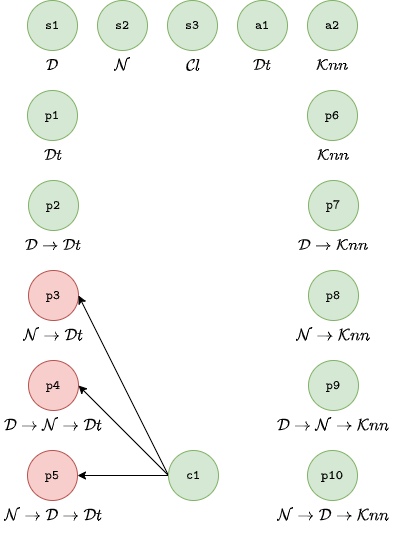
\includegraphics[width=\textwidth]{chapters/human-centric/hamlet/img/toy_example1.png}
        \caption{}
        \label{hamlet-fig:running_a}
    \end{subfigure}
    \hfill
    \begin{subfigure}[b]{0.3\textwidth}
        \centering
        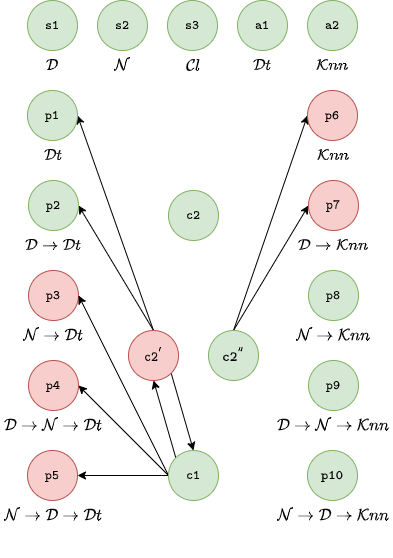
\includegraphics[width=\textwidth]{chapters/human-centric/hamlet/img/toy_example2.png}
        \caption{}
        \label{hamlet-fig:running_b}
    \end{subfigure}
    \hfill
    \begin{subfigure}[b]{0.3\textwidth}
        \centering
        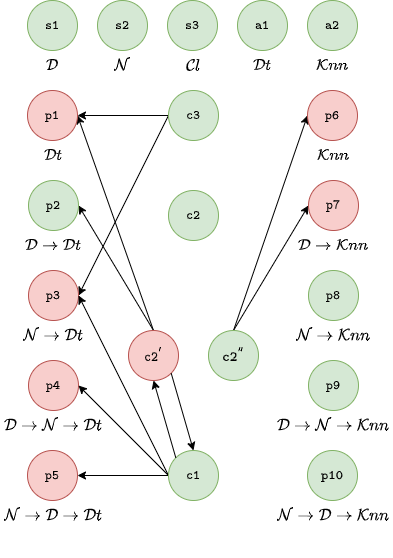
\includegraphics[width=\textwidth]{chapters/human-centric/hamlet/img/toy_example3.png}
        \caption{}
        \label{hamlet-fig:running_c}
    \end{subfigure}
    \caption{Examples of Problem Graphs. Green nodes are valid arguments, red ones are refuted. Arrows are attacks.}
    \label{hamlet-fig:toy_example}
\end{figure*}

When applying constraints, they can be conflicting.
We reify the constraints from \Cref{constraints} through conflict function in the Structured Argumentation domain-

\begin{definition}[AutoML Conflict]\label{conflictauto}
The conflict function $c_{ML}$ is a function from $L_{ML}$ to $2^{L_{ML}}$ that given a statement from $L_{ML}$ returns the set of conflicting statements.
\end{definition}

We support both the AutoML conflicts on ``pipeline vs constraint'' and ``constraint vs constraint''. 
Formally, let us consider two lists of steps $\alpha = \langle \ldots, S_i, S_j, \ldots \rangle$ and $\beta = \langle \ldots, S_y, S_x, \ldots \rangle$.
\begin{itemize}
    \item Pipeline vs constraint: return the constraints conflicting with pipelines.
    \begin{align*}
    c_{ML}&(pipeline(\beta, A)) = \\
        &\{mandatory(\alpha, A)~|~\exists S_i \in \alpha~s.t.~S_i \notin \beta\}~\cup \\
        &\{forbidden(\alpha, A)~|~\forall S_i \in \alpha,~S_i \in \beta \}~\cup\\
        &\{mandatory\_order(\alpha, A)~|~\exists S_i, S_j \in \alpha, S_x, S_y \in \beta, \\&\qquad\qquad\qquad S_i = S_x, S_j = S_y~s.t.~i < j, x > y\}
    \end{align*}
    Intuitively, a pipeline $pipeline(\langle S_i, S_j \rangle, A)$ is conflicting with a $mandatory$ constraint if the pipeline does not contains at least a mandatory step (e.g., the pipeline is conflicting with $mandatory(\langle S_j, S_k \rangle, A)$), with a $forbidden$ constraint if the pipeline contains all the forbidden steps (e.g., the pipeline is conflicting with $forbidden(\langle S_j \rangle, A)$), and with a $mandatory\_order$ constraint if the pipeline contains at least two steps that are not in the mandatory order (e.g., the pipeline is conflicting with $mandatory\_order(\langle S_j, S_i \rangle, A)$).
    \item Constraint vs constraint: return the constraints conflicting with other constraints.
    \begin{align*}
        c_{ML}&(forbidden(\beta, A)) = \{mandatory(\alpha, A)~|~\forall S_j \in \beta, S_j \in \alpha\}\\
        c_{ML}&(mandatory(\beta, A)) = \{forbidden(\alpha, A)~|~\forall S_j \in \alpha, S_j \in \beta\}\\
        c_{ML}&(mandatory\_order(\beta, A)) = \\
        &\{mandatory\_order(\alpha, A)~|~\exists S_i, S_j \in \alpha, S_x, S_y \in \beta, \\&\qquad\qquad\qquad S_i = S_x, S_j = S_y~s.t.~i < j, x > y\}
    \end{align*}
    Intuitively, $mandatory$ and $forbidden$ constraints are in conflict if all the forbidden steps are included in the mandatory constraint (i.e.,  $mandatory(\langle S_i, S_j, S_k \rangle, A))$ and a $forbidden(\langle S_i, S_j \rangle, A))$), this hold symmetrically for $forbidden$ and $mandatory$ constraints. Two $mandatory\_order$ constraints are in conflict if they contain at least two steps in different order (i.e.,  $mandatory\_order(\langle S_i, S_j, S_k \rangle, A))$ and a $mandatory\_order(\langle S_j, S_i \rangle, A))$).
\end{itemize}


\begin{example}[AutoML conflict]
With reference to the LogicalKB in \Cref{ex:kb}, let us consider the set of rules that represent the pipelines related to $\altmathcal{D}t$:
\begin{lstlisting}[mathescape=true]
# pipeline ending with a DT
p1 : $\Rightarrow$ pipeline($\altmathcal{D}t$).
# Discretization and DT
p2 : $\Rightarrow$ pipeline($\langle\altmathcal{D}\rangle$, $\altmathcal{D}t$).
# Normalization and DT
p3 : $\Rightarrow$ pipeline($\langle\altmathcal{N}\rangle$, $\altmathcal{D}t$).
# Discretization, Normalization, and DT
p4 : $\Rightarrow$ pipeline($\langle\altmathcal{D}$, $\altmathcal{N}\rangle$, $\altmathcal{D}t$).
# Normalization, Discretization, and DT
p5 : $\Rightarrow$ pipeline($\langle\altmathcal{N}$, $\altmathcal{D}\rangle$, $\altmathcal{D}t$).
\end{lstlisting}
In this case, \texttt{c1} (i.e., ``forbid $\altmathcal{N}$ in pipelines with $\altmathcal{D}t$'') is in conflict with the \emph{pipeline} statements \texttt{p3}, \texttt{p4}, and \texttt{p5} since they contain $\altmathcal{N}$ and $\altmathcal{D}t$.
\label{ex:conflict}
\end{example}

To create a Problem Graph, which is the medium readable by users and machines, we informally (for the sake of conciseness) introduce the key elements from Structured Argumentation; a complete formalization is available in \cite{Modgil2014aspic+}.
Given an Argumentation theory, an \emph{argument} is created for every rule with no premises (e.g., from the rule $r : \Rightarrow c$, we derive an argument with \emph{conclusion} $c$ using $r$).
Then, we recursively apply the other rules in the theory to the newly generated argument (e.g., we can use the argument with conclusion $c$ and the following rule $r1 : c \Rightarrow d$ to conclude an argument for $d$ using $r$ and $r1$).
This is repeated until no new argument can be generated.
In the rest of the paper we will refer to an argument with the set of rules used to generate it (e.g., given $r : \Rightarrow c$ and $r1 : c \Rightarrow d$, we will write $r$ and $r1$ when referring to the rules and $\{r\}$ and $\{r, r1\}$ for -- respectively -- the argument with \emph{conclusion} $c$ using $r$ and the argument with \emph{conclusion} $d$ using $r$ and $r1$).

An \emph{Argumentation framework} is defined using the arguments built from an Argumentation theory and their \emph{attack} relations.
Attacks are inconsistencies between arguments' conclusions and are computed using a conflict function (\Cref{conflictauto}).
For instance, given two arguments concluding respectively $a$ and $b$, and the conflict function $c$ such that $c(a) = \{b\}$, then the argument for $b$ directly attacks the one for $a$ (i.e., $b$ is in conflict with $a$).
The attack is propagated to all the arguments built over the receiver of the attack (e.g., if $a_1$ directly attacks $a_2$, and $a_2$'s conclusion is used to derive $a_3$, then $a_1$ also attacks $a_3$).
Also, we can define a \emph{preference} relation over arguments using a partial ordering over the rules in the Argumentation theory:
it is impossible for an argument to be attacked by the least preferred ones, even if they are in conflict.
In other words, we can explicitly solve inconsistencies in the LogicalKB using priorities.
We exploit the \emph{last-weakest} ordering as in \cite{Modgil2014aspic+}.

Finally, the evaluation of an Argumentation framework is performed through semantics, which determines all the sets of arguments that are consistent (called \emph{extensions}) in an Argumentation framework.
We exploit grounded semantics \cite{Dung1995abstractArg} to produce a \emph{grounded extension}; this semantics is the most skeptical---i.e., it includes only the arguments that are verified by all the possible interpretations. % of the graph.

\begin{definition}[Problem Graph]
We call \emph{Problem Graph} a graph in which nodes are arguments and edges are attacks from the Argumentation framework that is built on the Argumentation theory $\langle L_{ML}, LogicalKB \rangle$ and the conflict function $c_{ML}$.
\end{definition}

The benefits of the Problem Graph are two-fold.
First of all, it can be leveraged by both data scientists and domain experts to: understand, summarize and visualize the current knowledge.
Second of all, it is straightforward to convert such a graph of constraints into a space of possible solutions (i.e., exploiting Argumentation semantics, it is easy to obtain all the sets of arguments -- constraints and pipelines -- which hold together).

\begin{example}[Problem Graph]
\Cref{hamlet-fig:toy_example}a illustrates the Problem Graph extracted from the LogicalKB introduced in \Cref{ex:kb,ex:conflict} and evaluated under grounded semantics.
Arguments are represented as nodes, attacks as arrows and the colors represent the state of the arguments according to the semantics: red for refuted arguments, and green for the ones in the extension.
The arguments are identified through the set of rules used to build them.
In the upper part of the figure, we have a group of undefeated arguments, namely \texttt{\{s1\}}, \texttt{\{s2\}}, \texttt{\{s3\}}, \texttt{\{a1\}}, and \texttt{\{a2\}}, representing the basic knowledge used to setup the AutoML search space (i.e. steps and algorithms).
Then, we have an argument for every pipeline in \Cref{ex:conflict}: from \texttt{\{p1\}} to \texttt{\{p5\}} the pipelines regarding $\altmathcal{D}t$, from \texttt{\{p6\}} to \texttt{\{p10\}} the ones regarding $\altmathcal{K}nn$.
Finally, we can observe three different attacks: from \texttt{\{c1\}} to \texttt{\{p3\}}, \texttt{\{p4\}}, and \texttt{\{p5\}}, in accordance with the conflicts identified in \Cref{ex:conflict}.
The arguments in the extension give us all the information that we should use during the AutoML optimization process -- i.e. we should discard all the pipelines refuted by the constraint argument ($\{c1\}$), and focus on the remaining part of the search space.
\label{ex:graph}
\end{example}

The use of Argumentation relieves the data scientist of the burden of manually considering all the effects of the possible constraints.
It is important to notice that, although the increased degree of automation, the Problem Graph allows the data scientist and domain experts to correct, revise, and supervise the process.
Accordingly, possible inconsistencies -- due to diverging constraints -- can be verified by the data scientist using her knowledge.

Any change in the LogicalKB translates into a change in the Problem Graph, allowing the data scientist and domain experts to visualize it and argue about it.
The revision of the Problem Graph is the key element in the process of augmenting the knowledge: the data scientist and domain experts can consult each other and discuss how the new insights relate to their initial knowledge.
Indeed, thanks to the nature of the Problem Graph, it would be extremely easy to identify new possible conflicts and supporting arguments.
Furthermore, AutoML can update the Problem Graph by extracting constraints from the performed exploration, and transposing them into the LogicalKB.
For instance, the data scientist may not have considered that the dataset contains missing values.
AutoML helps in identifying the new data-related constraint ``require Imputation ($\altmathcal{I}$) in all the pipelines'' and adds it to the LogicalKB ($mandatory(\langle \altmathcal{I} \rangle, \altmathcal{C}l)$).

The described process is compliant with and augments the CRISP-DM process.
The inferred/learned knowledge is automatically handled throughout iterations, supporting the data scientist in the whole analysis in a continuous revision of the constraints.
\vspace{2cm}

\section{HAMLET}\label{hamlet-sec:implementation}

\begin{figure*}[t]
\begin{lstlisting}[mathescape=true]
# given an algorithm, create a pipeline including only such algorithm
hc0 : algorithm($\altmathcal{C}l$, A) $\Rightarrow$ pipeline($\langle~\rangle$, A).
# given some steps and an algorithm, create a pipeline including such steps and algorithm
hc1 : step($S_1$),$\ldots$,step($S_n$), algorithm($\altmathcal{C}l$, A) $\Rightarrow$ pipeline($\langle S_1, \ldots, S_n \rangle$, A).
# given constraints on the Pre-processing steps required for Classification...
# ... apply this constraints to all Classification algorithms
hc2 : mandatory($\langle S_1, \ldots, S_n \rangle$, $\altmathcal{C}l$), algorithm($\altmathcal{C}l$, A) $\Rightarrow$ mandatory($\langle S_1, \ldots, S_n \rangle$, A).
hc3 : forbidden($\langle S_1, \ldots, S_n \rangle$, $\altmathcal{C}l$), algorithm($\altmathcal{C}l$, A) $\Rightarrow$ forbidden($\langle S_1, \ldots, S_n \rangle$, A).
hc4 : mandatory_order($\langle S_1, \ldots, S_n \rangle$, $\altmathcal{C}l$), algorithm($\altmathcal{C}l$, A) $\Rightarrow$ mandatory_order($\langle S_1, \ldots, S_n \rangle$, A).
\end{lstlisting}
\caption{A subset of rules from the LogicalKB.}
\label{rules-arg2p}
\end{figure*}

HAMLET iterates over three phases (\Cref{hamlet-fig:approach}): (i) the generation of Problem Graph and search space out of the LogicalKB, (ii) the exploration of the search space in compliance with the specified constraints, and (iii) the augmentation of the LogicalKB through a rule recommendation.

The framework is available at \url{https://github.com/QueueInc/HAMLET}, and it is composed of two sub-modules. 
The first, written in Kotlin and running on the JVM, exposes a graphical interface on which the data scientists can compile and revise the LogicalKB. 
The module is also responsible for the generation and evaluation of the Problem Graph; it implements the Structured Argumentation functionalities as specified in \Cref{hamlet-sec:problem} using \argtup{} \cite{arg2p-jlc}, an ASPIC\textsuperscript{+}-based Kotlin library.
The second module, written in Python, is responsible for performing the AutoML optimization and the extraction of the new constraints from the explored space.

\subsection{Generation of Problem Graph and Search Space}
In \Cref{hamlet-sec:problem}, we defined the LogicalKB as the set of rules specified by the data scientist using her knowledge.
The LogicalKB also includes a set of hard-encoded rules representing inferences necessary to characterize the AutoML problems.
These rules are joined to the ones defined by the data scientist and used to build the Problem Graph (i.e., Argumentation framework).

A subset of rules is shown in \Cref{rules-arg2p}.
The first two ($hc0$ and $hc1$) define how to automatically derive a pipeline using algorithms and steps.
The construction of pipelines can be completely automated and the data scientist should be dispensed from manually enumerating all the possible pipelines as in \Cref{ex:conflict}.
In particular, the correct set of rules is built dynamically using the steps and algorithms provided by the DS, then they are used to derive all the arguments for the possible pipelines.
The last three rules ($hc2, hc3$ and $hc4$) encode constraints -- mandatory, forbidden, mandatory\_order -- on all the available algorithms with a single statement (e.g., $mandatory(\langle \altmathcal{D} \rangle, \altmathcal{C}l)$): it will be automatically used by the framework to derive the constraints for all the specific algorithms in the theory.

\begin{example}[Hard-coded rules]
With reference to \Cref{ex:graph} and \Cref{rules-arg2p}, we add rule \texttt{c2} for a new data-related constraint.
\begin{lstlisting}[mathescape=true]
# mandatory Norm. in Class. pipelines
c2 : $\Rightarrow$ mandatory($\langle\altmathcal{N}\rangle$, $\altmathcal{C}l$)
\end{lstlisting}
From the rule \texttt{c2}, the hard-coded rules generate the two arguments
\texttt{c2' = \{c2, a1, hc2\}} (i.e., $mandatory(\langle\altmathcal{N}\rangle, \altmathcal{D}t)$) and \texttt{c2'' = \{c2, a2, hc2\}} (i.e., $mandatory(\langle\altmathcal{N}\rangle, \altmathcal{K}nn)$) that are specific for the Classification algorithms in the LogicalKB.

However, \texttt{\{c1\}} (i.e., $forbidden(\langle\altmathcal{N}\rangle, \altmathcal{D}t)$; is in conflict with \texttt{c2'}.
Depending on her experience, the data scientist decides to resolve the conflict by specifying an ordering over the rules in the LogicalKB.
Assuming that the data scientist prefers \texttt{c1} to \texttt{hc2},
the argument \texttt{\{c1\}} is preferred to \texttt{c2'} and the attack from the latter is not considered in the final graph.
\Cref{hamlet-fig:toy_example}b shows the updated graph.
Firstly, we observe the support relation between \texttt{\{c2\}} and the generated constraints \texttt{c2'} and \texttt{c2''}.
Since \texttt{\{c1\}} has no attackers, it is added to extension.
Consequently, \texttt{c2'} is refuted and the pipelines attacked by it are correctly reinstated.
\label{ex:hard_coded_rules}
\end{example}

Given the Problem Graph (we recall that the Problem Graph contains \emph{all} the generated pipelines -- including their partial permutations), the search space can be extracted as in \Cref{spacealgorithm}. 
We iterate over all the generated pipelines in the Problem Graph and we recursively build their domain: the pipeline domain is the Cartesian product of the step domains, the step domain is the disjoint union of the algorithm domains (we leverage the disjoint union since each algorithm can be picked as an alternative to the others), the algorithm domain is the Cartesian product of its hyperparameters; the domain of a hyperparameter is given by definition.
Finally, the search space is the disjoint union of all the alternative pipeline domains.

Noticeably, while the search space could be constrained during its construction (e.g., by simply adding an ``if'' condition to check the validity of each pipeline at \Cref{spacealgorithm} line 10), current AutoML frameworks leverage optimization techniques that do not allow the explicit exclusion of regions from the search space.
As a consequence, we need to produce the entire search space first.

\begin{algorithm}[t]
\caption{Search Space from the Problem Graph}
\label{spacealgorithm}
\footnotesize
\begin{algorithmic}[1]
\Require{PG(N, E): Nodes and Edges of a Problem Graph}
\Ensure{$\Lambda$: Search Space}
    \item[]
    \Procedure{GetDomain}{$A$}
        \State $\Lambda_A \leftarrow \varnothing$
        \ForEach{$h \in A$} \Comment{For each hyperparameter in the algorithm...}
            \State $\Lambda_A \leftarrow \Lambda_A \times \Lambda_h$ 
            \Comment{Compute Cartesian product of hyperpar. domains}
        \EndFor
        \State \Return $\Lambda_A$ \Comment{Return the algorithm domain}
    \EndProcedure
    \item[]
    \State $\Lambda \leftarrow \varnothing$ \Comment{Initialize the search space}
    \ForEach{$pipeline(\alpha, A) \in N$} \Comment{For each argument that is a pipeline with $\alpha$ steps and alg. $A$...}
        \State $ \Lambda_{P} \leftarrow \textup{GetDomain(A)}$ \Comment{Init. pipeline domain with algorithm domain}
        \ForEach{$S \in \alpha$}  \Comment{For each step in the pipeline...}
            \State $\Lambda_{S}  \leftarrow \varnothing$ \Comment{Init. the step domain}
            \ForEach{$A \in S$}  \Comment{For each algorithm in the step...}
                \State $\Lambda_{S} \leftarrow \Lambda_{S} \cupdot \textup{GetDomain(A)}$ \Comment{Add alg. to step domain}
            \EndFor
            \State $\Lambda_P \leftarrow \Lambda_P \times \Lambda_S$ \Comment{Add step domain to pipeline domain}
        \EndFor
        \State $\Lambda \leftarrow \Lambda \cupdot \Lambda_P$ \Comment{Add pipeline domain to the search space}
    \EndFor
    \State \Return $\Lambda$ \Comment{Return the search space}
\end{algorithmic}
\end{algorithm}

\subsection{Exploration of a Constrained Search Space}\label{subsec:constrained_automl}

The Problem Graph is not only used to build the entire search space but it is also evaluated to understand which pipelines are invalid and which constraints are valid.
Hence -- through the Problem Graph -- we enhance AutoML exploration by combining the following techniques.
\begin{itemize}
    \item[(i)] Invalid pipelines are used to discourage the exploration of such a portion of the search space (we recall that a pipeline has a domain -- a region of the search space -- in which several pipeline instances are parametrized).
    First, we sample such regions of the search space, then we enforce a knowledge injection mechanism through warm-starting (i.e., the process of providing previous evaluations that help the model to converge faster).
    For instance, with reference to \Cref{ex:hard_coded_rules}, we sample some pipeline instances from the pipelines that have been discarded (from \texttt{\{p3\}} to \texttt{\{p7\}});
    then, we label such samples as invalid and provide them to the AutoML tool, helping the optimization algorithm to focus only on the valid portions of the space.
    \item[(ii)] Valid constraints -- expressed as conjunctions of Boolean clauses -- are used to discard the invalid pipeline instances that still are encountered by the AutoML tool.
    Indeed, since the sampling from (i) is non-exhaustive, it can happen that small portions of invalid regions could still be explored.
\end{itemize}

Our AutoML implementation is based on FLAML \cite{wang2021flaml}, which mixes Bayesian Optimization with CFO (Frugal Optimization for Cost-related Hyperparameters).
In a standard Bayesian process, an increasingly accurate model is built on top of the previously explored pipeline instances to suggest the most promising ones among the remaining.
The pipeline instances keep being explored, updating the model, until a budget in terms of either iterations or time is reached.
With CFO, there is also an estimation of the evaluation time to consider the frugality of the suggested pipeline instances -- hence favoring the ones requiring a smaller amount of time.
Throughout the exploration, different solutions are tested, which contribute to augmenting the global knowledge about the problem.

\subsection{Knowledge Augmentation through Rule Recommendation}

New constraints are automatically mined out of the pipeline instances explored by AutoML and \emph{recommended} in our logical language as rules.
Then, the data scientist decides which rules are accepted and added to the LogicalKB.


At this stage, we leverage frequent pattern mining techniques to learn constraints in an unsupervised manner.
Frequent pattern mining is the task of finding the most frequent and relevant patterns in large datasets (e.g., finding the products frequently bought together in the domain of market basket analysis); depending on the constraint type, we look for (sub)sets \cite{srikant1995mining} or (sub)sequences \cite{srikant1996mining} frequently recurring among the explored pipelines.
Since a pipeline instance is a sequence of algorithms, the set of the explored pipeline instances can be directly mapped into a transactional dataset \cite{srikant1995mining} where each pipeline instance is a transaction and each step -- inferred from the algorithm -- is an item.

We recommend the same constraints we support at the Argumentation level (i.e., $mandatory$, $forbidden$, $mandatory\_order$) so that AutoML can be as expressive as the DS.
For mandatory and forbidden constraints we look for (sub)sets \cite{srikant1995mining} frequently recurring among the explored pipelines.
Specifically, we split the explored pipeline instances by the applied Classification algorithm, set a minimum frequency (i.e., support) threshold to 50\% (i.e., to be retrieved, a set/sequence must occur at least in 50\% of the explored instances), and extract frequent maximal\footnote{Maximal itemsets are patterns that are not contained in any other.
For instance, given two frequent patterns, $\{a, b, c\}$ and $\{a, b\}$, the former is maximal while the latter is not.
}
itemsets.
The recommendation depends on the constraint.
\begin{itemize}
    \item $mandatory$: we consider only the patterns with good performance (i.e., $0.7 \leq metric \leq 1.0$); 
    \item $forbidden$: we consider only the patterns with bad performance (i.e., $0.0 \leq metric \leq 0.3$);
    \item $mandatory\_order$: the same considerations of the mandatory constraints stand, except that we look for (sub)sequences \cite{srikant1996mining} of length 2 to discover ordering dependencies in pairs of steps as in \cite{giovanelli2021data}.   
\end{itemize}
We leveraged well-known implementations \cite{raschkas_2018_mlxtend} and \cite{seq2pat2022} for itemsets and sequences mining, respectively.
Finally, we return to the data scientist only the top-10 rules sorted by descending support; we allow the data scientist to explore all the rules on-demand.

The thresholds act as filters on the extracted rules since we cannot burden the user with the investigation of hundreds of recommendations. 
As to the intervals, our rationale is simple: we only want to recommend as mandatory (order) the rules that achieved ``good performance'' and as forbidden the rules that achieved ``bad performance''.
Since we handle classification pipelines that mainly refer to (balanced) accuracy/F1 score/recall, we mapped ``good'' in the interval $[0.7, 1.0]$ and ``bad'' in the interval $[0, 0.3]$. For the frequent pattern extraction, we consider only the pipeline instances falling in these intervals.
As to the support, 50\% ensures that the pattern recurs on many of the explored instances and empirically showed to be a good threshold to have good efficiency in the extraction of frequent patterns.

\begin{example}[Rules Recommendation]
With reference to the Problem Graph in \Cref{ex:hard_coded_rules},
the AutoML results are filtered according to the chosen metric, the algorithm \cite{raschkas_2018_mlxtend} is applied, and let us assume that the rule \texttt{c3} is recommended:
\begin{lstlisting}[mathescape=true]
c3 : $\Rightarrow$ mandatory($\langle\altmathcal{D}\rangle$, $\altmathcal{D}t$).
\end{lstlisting}
The constraints specifies ``mandatory $\altmathcal{D}$ in pipelines with $\altmathcal{D}t$''.
As a matter of fact, it is well known that Discretization improves the performance of tree-based algorithms giving to them the ability to apply multiple split in the decision nodes.
\Cref{hamlet-fig:toy_example}c shows the effect of the applied constraint: a new portion of the search space is excluded from the extension ($\{p1\}$).
\end{example}


\section{Experimental Evaluation}\label{hamlet-sec:test}

The performance of HAMLET depends on (i) the rules encoded in the LogicalKB and (ii) the rules recommended after each run.
To test both the effectiveness and efficiency of our approach, we define three experimental settings.
\begin{itemize}
    \item PKB (Preliminary Knowledge Base), HAMLET starts with a preliminary LogicalKB constraining the search space from the first iteration, and no rule mining is applied.
    %, but the rules that are suggested throughout the iterations are not applied.
    The preliminary LogicalKB consists of the rules discovered in \cite{giovanelli2021data} and some well-known from the literature (e.g., suggested by scikit-learn\footnote{\url{https://scikit-learn.org/stable/auto_examples/preprocessing/plot_discretization.html}}).
    The complete knowledge base can be found in the Github repository.
    \item IKA (Iterative Knowledge Augmentation), HAMLET starts with an empty LogicalKB, and all the rules recommended after each run are applied to extend the LogicalKB.
    \item PKB+IKA, HAMLET starts with a preliminary LogicalKB, and the rules recommended after each run are applied to extend the LogicalKB.
\end{itemize}
HAMLET run 4 times in every setting -- intuitively, four runs of knowledge augmentation -- the budget assigned to each run is 125 pipeline instances in 900 seconds (15 minutes).
We also test against a baseline: we let AutoML explore 500 pipeline instances ($= 125 \cdot 4$) in a single run with a time budget of 3600 seconds ($= 900 \cdot 4$; 1 hour).

For such an evaluation, we derive a search space out of 6 steps, 5 Data Pre-processing steps (Imputation, Normalization, Discretization, Feature Engineering, and Rebalancing) followed by the final Classification task.
Since the tests are run on datasets from OpenML \cite{OpenML2013} -- a well-known repository for data acquisition and benchmarking -- and it provides already-encoded datasets, we do not consider the encoding step. 
Except for that, we included all the Data Pre-processing steps and algorithms available in the scikit-learn \cite{scikit-learn} Python library (plus imbalance-learn \cite{JMLR:v18:16-365} for Rebalancing transformations).
The leveraged steps, algorithms per step, and hyperparameters per algorithm are reported in \Cref{hamlet-tbl:search_space}.

\begin{table}[t]
    \footnotesize
    \caption{Algorithms and number of hyperparameters for each of the steps in HAMLET. Algorithm names and hyperparameters are imported from the scikit-learn Python library.}
    \centering
    \begin{tabular}{llc}
        \toprule
        \textbf{Step} & \textbf{Algorithm} & \textbf{\#Hyperparameters}  \\\midrule
        Imputation        & SimpleImputer & 1 \\
                          & IterativeImputer & 2 \\
        Normalization     & StandardScaler & 2 \\
                          & MinMaxScaler & 0 \\
                          & RobustScaler & 2 \\
                          & PowerTransformer & 0 \\
        Discretization    & Binarizer & 1 \\
                          & KBinsDiscretizer & 3 \\
        Feature Eng.      & SelectKBest & 1 \\
                          & PCA & 1 \\
        Rebalancing       & NearMiss & 1 \\
                          & SMOTE & 1 \\
        Classification    & DecisionTreeClassifier & 7 \\
                          & KNeighborsClassifier & 3 \\
                          & RandomForestClassifier & 7 \\
                          & AdaBoostClassifier & 2 \\
                          & MLPClassifier & 6 \\ \bottomrule
    \end{tabular}
    \label{hamlet-tbl:search_space}
\end{table}

The OpenML-CC18 suite is a well-known collection of 72 datasets for benchmarking.
Given the time-consuming computation of each dataset (8 hours per dataset = 2 hours for the baseline + 6 hours for HAMLET in the three settings) -- in this preliminary evaluation -- we select a representative subset of datasets according to three meta-features provided by OpenML: number of instances, number of features, and number of classes.
For each of the considered meta-features, we search for datasets with either high or low values, and we select the representatives that maximize the overall dataset diversification.
\Cref{hamlet-tbl:datasets} illustrates the 6 datasets that have been identified; note that some combinations of meta-features have no representative dataset in the suite.
Among these, we do not report the results for the dataset mnist\_784 since the number of explored pipeline instances is insufficient to validate the result (i.e., due to the time necessary to run a single pipeline instance, only 50 instances were explored out of 1000).

\begin{table}[t]
    \caption{Dataset descriptions.}
    \footnotesize
    \label{hamlet-tbl:meta_features}
    \begin{threeparttable}
    \centering
        \begin{tabular}{ll|ll|ll|ll}
            \toprule
             \textbf{OpenMLID} \tnote{a} & \textbf{Dataset} & \multicolumn{2}{c}{\textbf{Instances}} & \multicolumn{2}{c}{\textbf{Features}} & \multicolumn{2}{c}{\textbf{Classes}}  \\ \midrule
             40983 & wilt & 4839 & \footnotesize{\texttt{L}} & 6 & \footnotesize{\texttt{L}} & 2 & \footnotesize{\texttt{L}}\\
             40499 & texture & 5500& \footnotesize{\texttt{L}} & 41& \footnotesize{\texttt{L}} & 11& \footnotesize{\texttt{H}}\\
             1485 & madelon & 2600 & \footnotesize{\texttt{L}} & 501 & \footnotesize{\texttt{H}} & 2 & \footnotesize{\texttt{L}}\\
             1478 & har & 10229 & \footnotesize{\texttt{L}} & 562& \footnotesize{\texttt{H}} & 6& \footnotesize{\texttt{H}}\\
             1590 & adult & 48842& \footnotesize{\texttt{H}} & 9& \footnotesize{\texttt{L}} & 2& \footnotesize{\texttt{L}}\\
             -- & -- & -- & \footnotesize{\texttt{H}} & -- & \footnotesize{\texttt{L}} & -- & \footnotesize{\texttt{H}}\\%[-1.5ex]\hline\noalign{\vspace{\dimexpr 2.ex-\doublerulesep}}
             -- & -- & -- & \footnotesize{\texttt{H}} & -- & \footnotesize{\texttt{H}} & -- & \footnotesize{\texttt{L}}\\%[-1.5ex]\hline\noalign{\vspace{\dimexpr 2.ex-\doublerulesep}}
             554 & mnist\_784 & 70000& \footnotesize{\texttt{H}} & 785& \footnotesize{\texttt{H}} & 10& \footnotesize{\texttt{H}}\\%[-1.5ex]\hline\noalign{\vspace{\dimexpr 2.ex-\doublerulesep}}
             \bottomrule
        \end{tabular}
        \label{hamlet-tbl:datasets}
        \begin{tablenotes}
            \item[--] {\scriptsize Not Applicable}
            \item[\texttt{H}] {\scriptsize The value $v$ is high for the meta-feature $F$ if $ v \geq \frac{1}{|F|}\sum_{f \in F} f$}
            \item[\texttt{L}] {\scriptsize The value $v$ is low for the meta-feature $F$ if $v < \frac{1}{|F|}\sum_{f \in F} f$}
            \item[a] {\scriptsize Datasets are available at \url{https://www.openml.org/d/<OpenMLID>}}
        \end{tablenotes}
    \end{threeparttable}
\end{table}

\subsection{Effectiveness}
\begin{figure}[t]
    \centering
    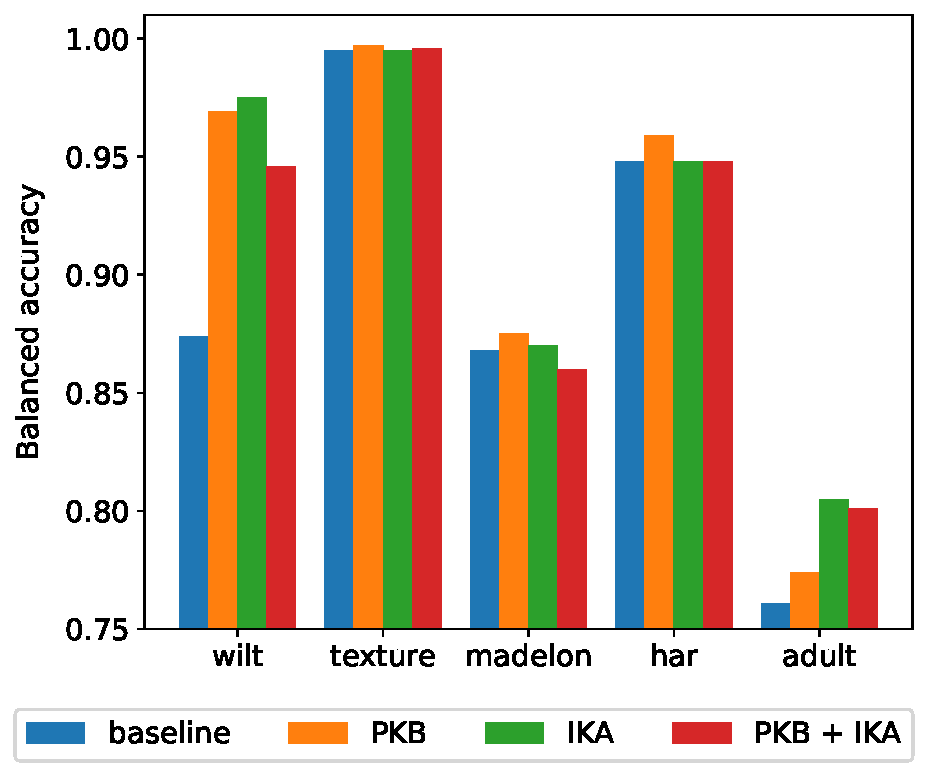
\includegraphics[scale=.45]{chapters/human-centric/hamlet/img/accuracy.pdf}
    \caption{Results assessing the effectiveness of HAMLET w.r.t. the baseline.}
    \label{hamlet-fig:effectiveness}
\end{figure}

\begin{figure}[h!]
    \RawFloats
    \centering
    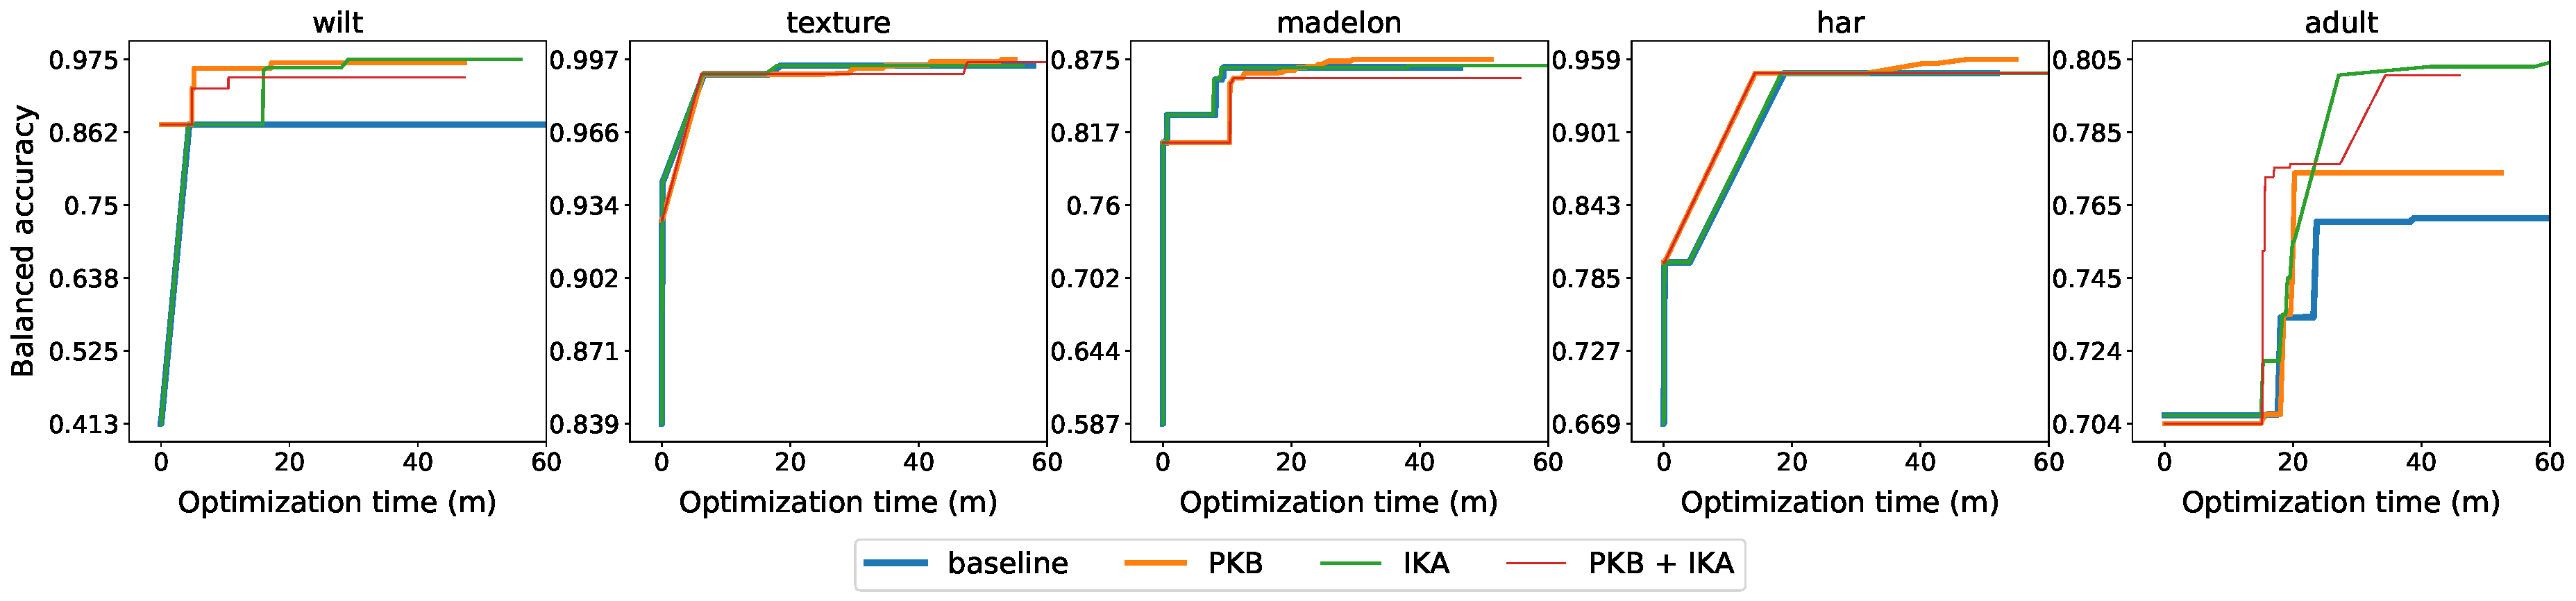
\includegraphics[scale=.25]{chapters/human-centric/hamlet/img/accuracy_time.pdf}
    \caption{Results assessing the performance of HAMLET through the optimization time.}
    \label{hamlet-fig:efficiency}
    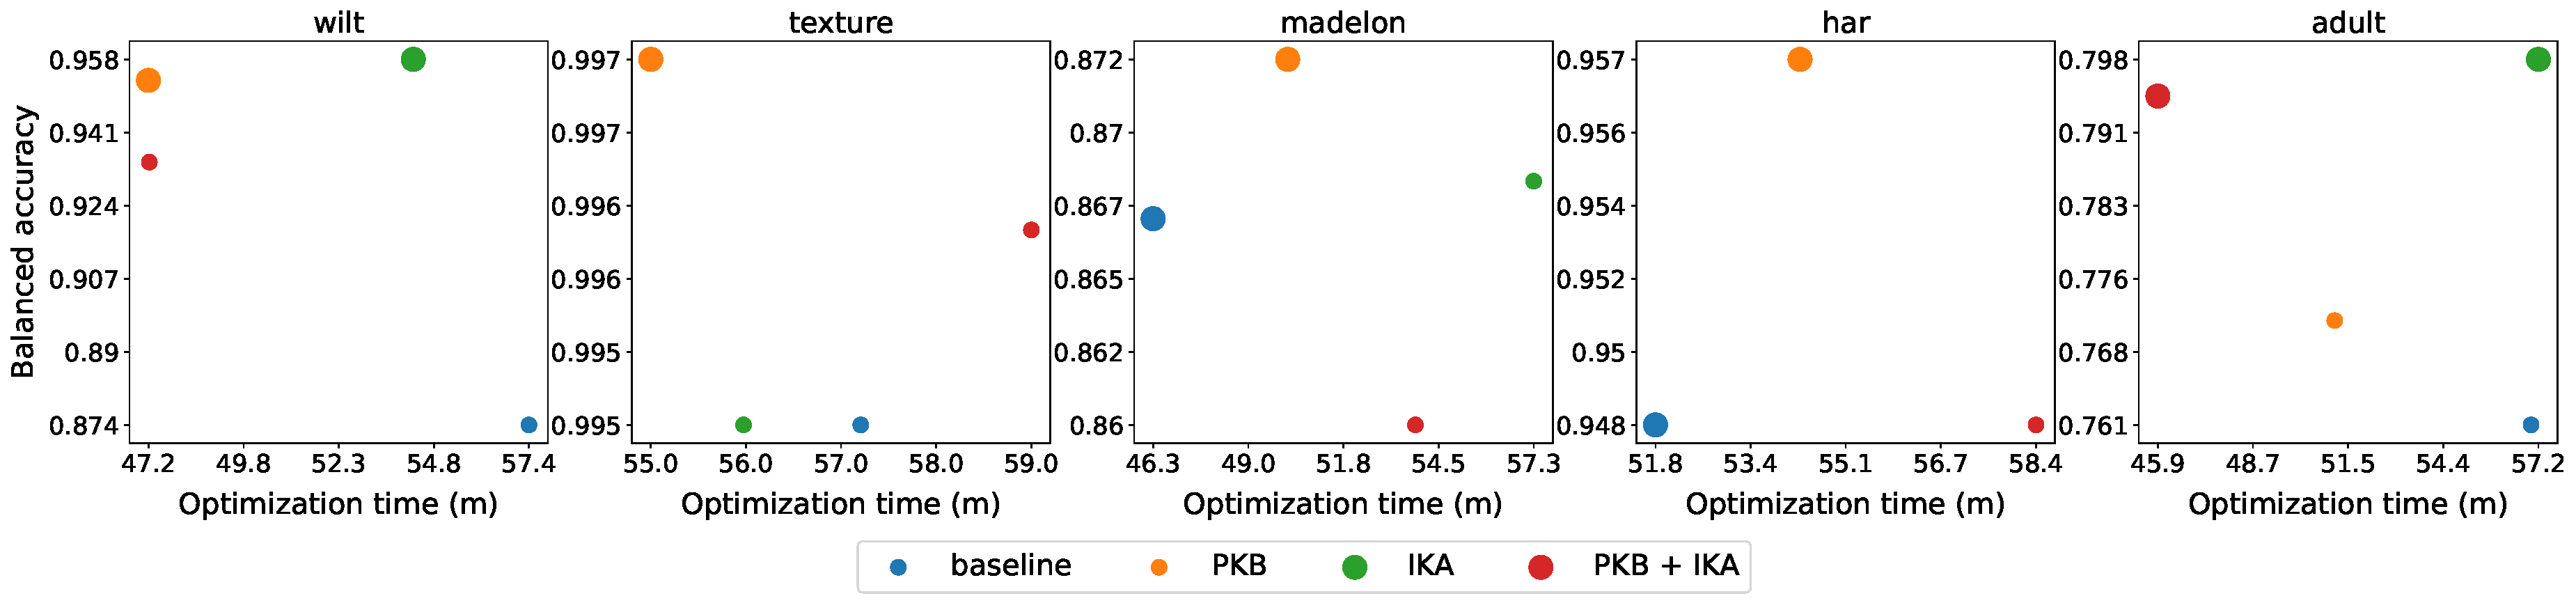
\includegraphics[scale=.25]{chapters/human-centric/hamlet/img/skyline.pdf}
    \caption{Comparison of the best pipeline instances characterized by optimization time and (balanced) accuracy, bigger circles represent settings that dominate the others.}
    \label{hamlet-fig:effskyline}
\end{figure}

We employ balanced accuracy as the quality metric.
For instance, in case of (two) binary classes, such a score is
$$
\texttt{Balanced accuracy} = \frac{1}{2}\left ( \frac{TP}{TP + FN} + \frac{TN}{TN + FP}\right )
$$
where $TP$ and $TN$ stand respectively for True Positive and True Negative (i.e., number of instances that have been correctly assigned to the positive and negative classes), and $FP$ and $FN$ stand respectively for False Positive and False Negative (i.e., number of instances that have been mistakenly assigned to the positive and negative classes). The formulation generalized to more than 2 classes can be found at \cite{DBLP:conf/icpr/BrodersenOSB10}.
The score avoids inflated performance estimations on imbalanced datasets.
For balanced datasets, the score is equal to the conventional accuracy (i.e., the number of correct predictions divided by the total number of predictions), otherwise it drops to $\frac{1}{\#classes}$.

\Cref{hamlet-fig:effectiveness} illustrates the performance achieved by the baseline and the three settings of HAMLET.
HAMLET is clearly beneficial since in all datasets the framework overcomes the baseline.
The preliminary results highlight that both the LogicalKB and rule recommendation play important roles:
\begin{itemize}
    \item When we warm-start the exploration with a non-empty LogicalKB (PKB), in all datasets HAMLET overcomes the baseline.
    \item When we only leverage rule recommendation (IKA), we achieve results that are better than or equivalent to PKB, indeed we are injecting in the LogicalKB new rules that are tailored to the dataset.
    \item The synergy of PKB+IKA performs better than PKB in adult, worse in wilt, and the two are comparable in the other datasets.
    On the one hand, the PKB act as a warm start mechanism that speeds up the optimization; on the other hand, if not aligned with the recommended rules, it can mitigate the benefits of IKA.
    This proves to be a promising direction that further requires investigation since merging the words will require further studies.
    Indeed, it is worth noting that the recommended rules can be overlapping with the ones in the LogicalKB, highlighting the need to improve the recommendation process by also considering the rules that are already present in the LogicalKB.
\end{itemize}

In PKB+IKA, IKA can introduce rules that contradict the ones in the LogicalKB of PKB; for instance when the PKB contains rules that are not ``representative'' of the dataset/algorithms in use. We believe that this is an added value of HAMLET since ``incomplete'' (or even wrong) LogicalKBs can be corrected/refined by a data-driven approach. Finally, PKB+IKA and IKA are likely to produce different rules, since in PKB+IKA the LogicalKB biases the exploration of the search space from the beginning (acting as a warm start mechanism).

\subsection{Efficiency}


\Cref{hamlet-fig:efficiency} shows how settings converge to the optimal pipeline instance.
Noticeably, PKB and PKB+IKA start with higher accuracy than IKA and the baseline in four datasets out of five, proving how the preliminary LogicalKB warm starts the exploration.
However, time and \#iterations alone are not fair metrics for comparison; for instance, an optimization strategy could privilege simple algorithms taking small amounts of computational time but producing worse results than ``more complex'' algorithms.
In the direction of multi-objective optimization (exploration time should be minimized while accuracy should be maximized), \Cref{hamlet-fig:effskyline} depicts which settings dominate the others using the Skyline operator \cite{borzsony2001skyline}.
A setting dominates another one if it is as good or better in all dimensions (time and accuracy) and better in at least one dimension (time or accuracy).
PKB dominates in 80\% of the datasets, IKA in 40\%, PKB+IKA in 20\%, and the baseline in 40\%.
Noticeably, the baseline is selected as dominating only in madelon and har datasets due to the fact that converges faster than HAMLET (although it converges to a pipeline instance with lower accuracy).


\begin{figure}[t]
    \centering
    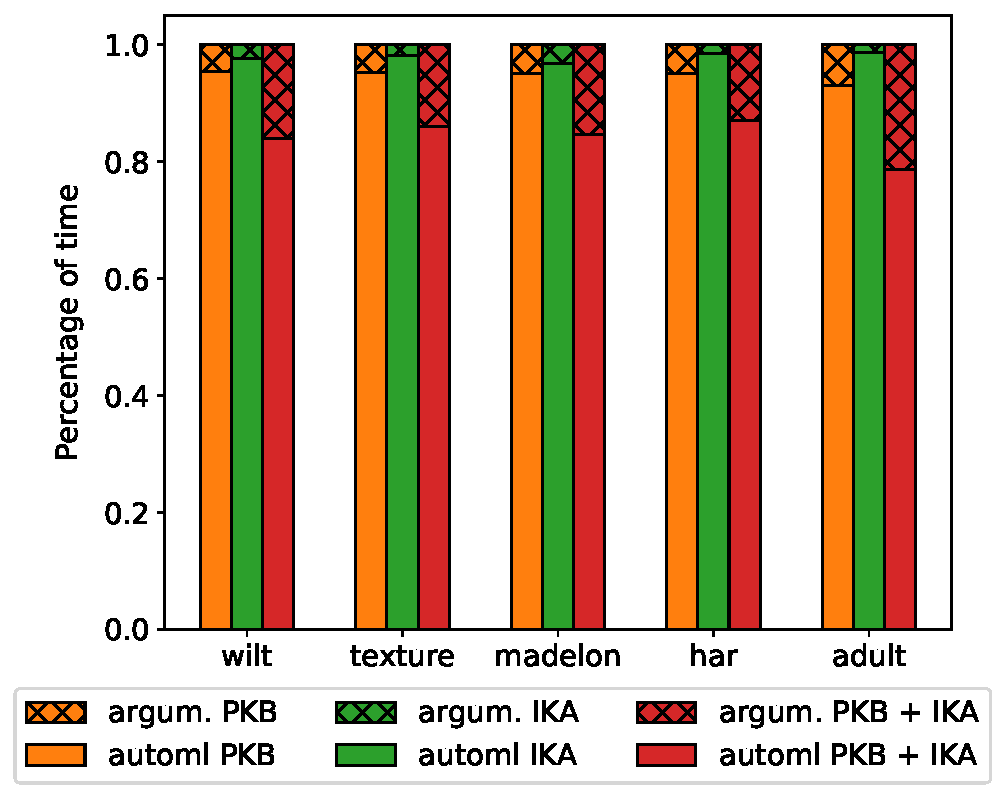
\includegraphics[scale=.43]{chapters/human-centric/hamlet/img/time.pdf}
    \caption{Computational time of the argumentation and AutoML processes.}
    \label{hamlet-fig:effoverhead}
\end{figure}


Finally, \Cref{hamlet-fig:effoverhead} depicts the overhead introduced by the argumentation framework in HAMLET that, at maximum, is 20\% of the computational time in the adult dataset.
This proves that the argumentation time is marginal with respect to the duration of the optimization process.
As expected, PKB+IKA shows the highest overhead since the number of rules to manage is the highest.

\subsection{Comparison}

\begin{figure}[t]
    \centering
    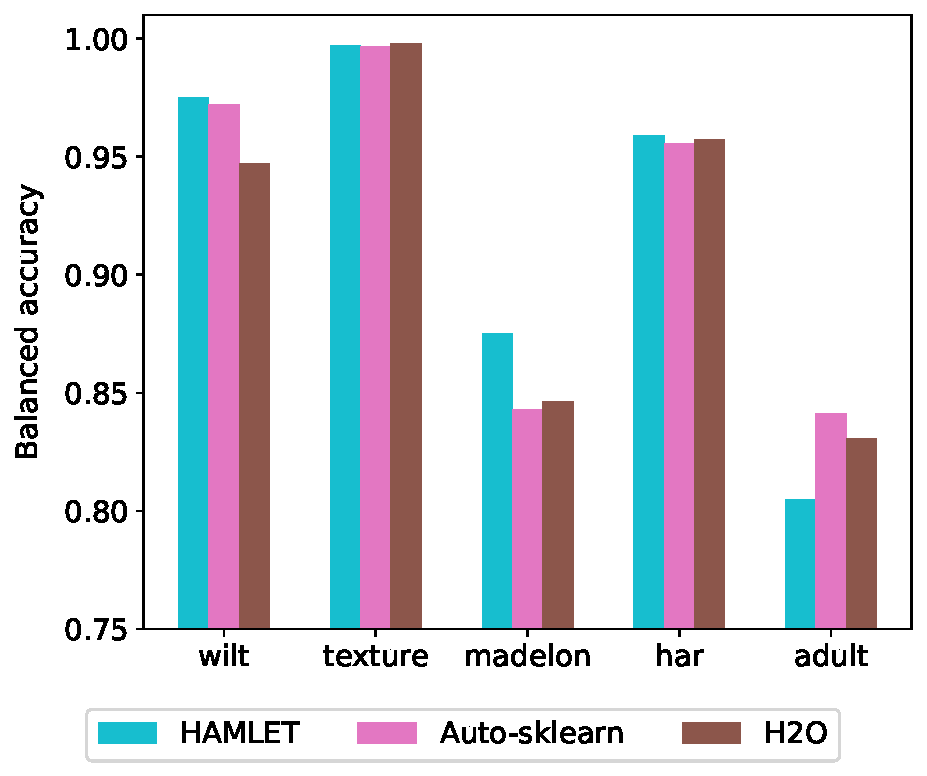
\includegraphics[scale=.45]{chapters/human-centric/hamlet/img/comparison.pdf}
    \caption{Results assessing the performance of HAMLET w.r.t. Auto-sklearn \cite{feurer2019auto} and H2O \cite{ledell2020h2o}.}
    \label{hamlet-fig:comparison}
\end{figure}


\Cref{hamlet-fig:comparison} compares HAMLET against two well-known AutoML frameworks: Auto-sklearn \cite{feurer2019auto} and H2O \cite{ledell2020h2o}.
In four datasets out of five, HAMLET outperforms or is comparable to the two frameworks.
Additionally, the added value of HAMLET is \textit{explainability}.
Hamlet is a human-in-the-loop AutoML framework tailored to the needs of data scientist that (i) enables the injection of their experience into the exploration process as well as (ii) the spreading and sharing of knowledge bases that encode what data scientists have understood by the optimization of their pipelines.


\section{Conclusions and Future Work}\label{hamlet-sec:conclusion}

Data platforms support Data Scientists in performing end-to-end data analysis; to this end, Machine Learning plays a primary role.
However, the complexity and heterogeneity of (Automated) Machine Learning processes are leading Data Scientists to lose control over such processes.
Human awareness about the constraints and solutions of Machine Learning tasks is a fundamental aspect to consider, and consequently, the Data Scientist should play a central role in the design of next-generation data platforms.

According to this vision, we present HAMLET, a framework for Human-centered AutoML based on Logic and Structured Argumentation.
Logic is exploited to structure the knowledge that the Data Scientist gathers while designing, modeling, and deploying a solution.
The logical encoding of the knowledge provides a medium that is both human- and machine-readable and it allows an easy exploration and verification of all the constraints that may apply to the case at hand---it is overwhelming for the Data Scientist to correctly handle the vast amount of them.
The preliminary evaluation of HAMLET shows promising results against state-of-the-art AutoML algorithms both in terms of effectiveness and efficiency, with argumentation introducing a small overhead with respect to the duration of the exploration process.

The directions for future work are plentiful, among them:
\begin{itemize}
    \item[(i)] the recommendation of more constraints out of the explored search space (e.g., rare or negative patterns);
    \item[(ii)] the support to heterogeneous constraints on hyperparameter domains;
    \item[(iii)] the injection of meta-learning into our Logical Knowledge Base to better identify when and how the constraints should be applied (e.g., this can be done after testing HAMLET on a multitude of datasets);
    \item[(iv)] the introduction of a visual metaphor (e.g., based on the Problem Graph) to help Data Scientists' understanding;
    \item[(v)] the study of automatic resolution/recommendation of conflicting constraints, also depending on the rules already embedded in the Logical Knowledge Base.
\end{itemize}

\chapter{Interactive Optimization in Multi-Objective via Preference Learning}
\label{human-centric-chap:moo}

Practical applications of machine learning often call for the optimization of more than one loss or objective function, called multi-objective machine learning (MO-ML) \cite{jin-momlbook06a} borrowing from the notion of multi-objective optimization (MO) \cite{deb-ds16,gunantara-ce18}.
For example, instead of only focusing on the performance of a model, its energy consumption is becoming more and more important in various domains such as edge computing, but also in general, sparked by efforts in the area of green artificial intelligence (Green AI) \cite{schwartz-arxiv19a,wynsberghe-aiethics21a}.
Comparing two ML models with respect to several objectives is non-trivial and most approaches solve this problem by returning a set of solutions that cannot be improved further without going to the expense of at least one of the objectives, called the Pareto front.
Naturally, as standard ML algorithms, MO-ML algorithms expose hyperparameters controlling their learning behavior and thus, also the resulting Pareto front.
To unleash the full potential of the MO-ML algorithms, these hyperparameters should be optimized with adequate methods.

\paragraph{Challenges} Unfortunately, optimizing the hyperparameters of such MO-ML algorithms is challenging for a user with standard hyperparameter optimization (HPO) \cite{feurer-automlbook19a,bischl-dmkd23a} approaches, such as SMAC \cite{hutter-lion11a,lindauer-jmlr22a}, Optuna \cite{akiba-kdd19a}, Hyperopt \cite{komer-scipy14a}, HpBandSter \cite{falkner-icml18a} or SyneTune \cite{salinas-automl22}, which iteratively evaluate configurations.
This is the case, as evaluating a hyperparameter configuration of an MO-ML algorithm involves evaluating the quality of the Pareto front of models returned by the corresponding algorithm.
Several so-called (quality) indicators, such as hypervolume \cite{zitzler1999multiobjective}, are used to assess different properties of the shape of the Pareto front and in principle can also be used for the purpose of rating a configuration in the context of HPO.
Nevertheless, although a user might have a clear idea about what kind of Pareto front shape they would like to choose their final model from, choosing the quality indicator leading to this Pareto front shape is a challenging task in practice. At the same time, however, correctly configuring the HPO tool with the right loss function, i.e. quality indicator in our case, is crucial to achieve the desired result.

\paragraph{Contributions} We propose an interactive human-centric HPO \cite{pfisterer-arxiv2019a,souza-ecmlpkdd21a,moosbauer-neurips21a,hvarfner-iclr22a,moosbauer-arxiv22a,segel-automl23a,mallik-arxiv23} approach for MO-ML algorithms that frees users from choosing a predefined quality indicator suitable for their needs by learning one tailored towards them based on feedback.
To achieve this, it first learns the desired Pareto front shape from the user in a short interactive session and then starts a corresponding HPO process optimizing towards the previously learned Pareto front shapes.
Instead of requiring the user to present us with a concrete Pareto front they would favor, we interactively and iteratively present them a few pairs of Pareto fronts asking them for their preferences.
Based on these pairwise comparisons, we leverage methods from the field of preference learning (PL) \cite{furnkranz-plbook10a} to learn a latent utility function serving as a Pareto front quality indicator customized to the user.
In the subsequent stage, we run a state-of-the-art HPO tool
instantiated with the learned Pareto front quality indicator to evaluate configurations and the corresponding Pareto fronts.

In summary, we make the following contributions:
\begin{itemize}
    \item We propose an interactive approach to learn a Pareto front quality indicator from pairwise comparisons based on a latent utility function with methods from the field of preference learning. This quality indicator is customized to the user and can be learned from a small number of pairwise comparisons. 
    \item We combine the aforementioned learned quality indicator with an HPO tool 
    to provide a full-fledged HPO approach for multi-objective MO-ML algorithms, which frees the user to choose an appropriate Pareto front quality indicator offering less opportunity for a mistake and thus, bad optimization results.
    \item In an experimental case study, we demonstrate that our approach leads to substantially better Pareto fronts compared to optimizing based on a wrong indicator pre-selected by the user, and performs comparable in case of an advanced user knowing which indicator to pick. Thus, our approach makes HPO for MO-ML algorithms substantially more easily and robustly applicable in practice.
\end{itemize}

The reminder of this chapter is structured as follows.
\Cref{moo-sec:background} refreshes the background on HPO, MO, and introduces preference learning;
\Cref{moo-sec:background_work} discusses the related works;
\Cref{moo-sec:method} details our approach; \Cref{moo-sec:evaluation} reports the extensive evaluation performed; and finally, \Cref{moo-sec:conclusion} draws the conclusions and future works.

\section{Background}
\label{moo-sec:background}

Since our work is spanned along the dimensions of hyperparameter optimization (HPO), multi-objective optimization (MO), and preference learning (PL), in the following, we refresh the formalization of the former two concepts (\Cref{moo-ssec:hpo} and \Cref{moo-ssec:moo} respectively) and introduce the latter (\Cref{moo-ssec:preference_learning_related}).

\subsection{Hyperparameter Optimization} \label{moo-ssec:hpo}
HPO formalizes the task of finding a hyperparameter configuration for a machine learning algorithm leading to a well-performing model on a given dataset 
\begin{equation}
    \altmathcal{D} = \{(\vec{x}_n, y_n)\}_{n=1}^N \in \mathbb{D} \subset \altmathcal{X} \times \altmathcal{Y}
\end{equation}
with an instance space $\altmathcal{X}$ and a target space $\altmathcal{Y}$. 
In addition to the dataset, we are provided with a hyperparameter configuration space $\boldsymbol{\Lambda} = \Lambda_1 \times \dots \times \Lambda_K$ with $K$ hyperparameters, where $\Lambda_k$ is the domain of the $k^{\mathit{th}}$ hyperparameter, and an algorithm $A: \mathbb{D} \times \vec{\Lambda} \rightarrow \altmathcal{H}$ which trains a model from the model space $\altmathcal{H}$ given a dataset and a hyperparameter configuration. 
Furthermore, we are provided with a loss function $\altmathcal{L}: \altmathcal{H} \times \mathbb{D} \rightarrow \mathbb{R}$ quantifying how well a given model performs on a given dataset. 
The loss function can be used to assess the quality of a hyperparameter configuration by splitting the original dataset $\altmathcal{D}$ into two disjoint datasets $\altmathcal{D}_\mathit{train}$ and $\altmathcal{D}_\mathit{test}$, where the model is trained only based on $\altmathcal{D}_\mathit{train}$ but evaluated with $\altmathcal{L}$ on $\altmathcal{D}_\mathit{test}$. 
Overall, we seek to find the optimal hyperparameter configuration $\vec{\lambda}^* \in \vec{\Lambda}$ defined as 
\begin{equation}\label{moo-eq:hpo}
    \vec{\lambda}^* \in \arg\min_{\vec{\lambda} \in \vec{\Lambda}} \altmathcal{L}\left( A \left( \altmathcal{D}_{\mathit{train}}, \vec{\lambda} \right), \altmathcal{D}_\mathit{test} \right) \, .
\end{equation}

There exist several approaches to automatically solving the optimization problem defined in \eqref{moo-eq:hpo}, many of which are powered by Bayesian optimization (BO) \cite{frazier-arxiv18a} or evolutionary approaches \cite{bischl-dmkd23a}. 
Most of these techniques internally iteratively evaluate a large set of configurations based on their true estimated loss. 
To this end, they split up a so-called validation dataset $\altmathcal{D}_\mathit{val}$ from the training dataset $\altmathcal{D}_\mathit{train}$ to estimate the loss $\altmathcal{L}(A(\altmathcal{D}_{\mathit{train}}, \vec{\lambda}), \altmathcal{D}_\mathit{test})$ of a configuration $\vec{\lambda}$ by $\altmathcal{L}(A(\altmathcal{D}_{\mathit{train}}, \vec{\lambda}), \altmathcal{D}_\mathit{val})$ and avoid a biased overfit to $\altmathcal{D}_\mathit{test}$.

\subsection{Multi-Objective Machine Learning}
\label{moo-ssec:moo}

When it comes to learning a machine learning model with more than one (possibly conflicting) objective or loss function $\altmathcal{L}_1, \dots, \altmathcal{L}_M$ in mind, comparing the quality of models becomes difficult. For instance, in the context of Green AI, searching for a model with higher performance usually leads to one with higher power consumption, and vice versa. Thus, in multi-objective ML, learning algorithms leverage the concept of dominance formalizing that one model $H_1 \in \altmathcal{H}$ is better than another $H_2 \in \altmathcal{H}$, if $H_1$ performs better in at least one of the objectives while not performing worse than $H_2$ in the remaining ones. Yet, this leaves us with a set of non-dominated models, which are indistinguishable with respect to this dominance idea. These models form a so-called Pareto front $P_{\altmathcal{D}_{\mathit{val}}}(H)$ evaluated on dataset $\altmathcal{D}_{\mathit{val}}$ for a given set of models $H \subset \altmathcal{H}$. Formally, a Pareto front is defined as

\begin{equation}
    \label{moo-eq:pareto_def}
        P_{\altmathcal{D}_{\mathit{val}}}(\altmathcal{H}) = \left\{ H \,\, \begin{array}{|l}
        H \in \altmathcal{H}, \nexists H' \in \altmathcal{H},
        \forall m \in \{1, \dots, M\} : \\
        \quad\quad\altmathcal{L}_m(H',\altmathcal{D}_{\mathit{val}}) \leq \altmathcal{L}_m(H,\altmathcal{D}_{\mathit{val}}), \\
        \exists j \in \{1, \dots, M\} : \\
        \quad\quad\altmathcal{L}_j(H',\altmathcal{D}_{\mathit{val}}) < \altmathcal{L}_j(H, \altmathcal{D}_{\mathit{val}})
        \end{array}\right\} \, .
    \end{equation}

Due to the problem of further distinguishing non-dominated models among each other, MO-ML algorithms usually resolve to returning the complete Pareto front of models instead of a single model. Thus, formally, the signature of an algorithm changes to $A: \mathbb{D} \times \vec{\Lambda} \rightarrow 2^{\altmathcal{H}}$. As a consequence, the evaluation of each hyperparameter configuration of such an MO-ML algorithm also involves quantifying the quality of a Pareto front of models instead of a single model returned by the algorithm, yielding a much more difficult problem. As such, the signature of our HPO loss function used in \Cref{moo-eq:hpo} also needs to change to $\altmathcal{L}: 2^{\altmathcal{H}} \times \mathbb{D} \rightarrow \mathbb{R}$ and thus can no longer be instantiated with simple loss functions such as accuracy. 

One way of assessing the quality of a Pareto front and thus instantiating the HPO loss function $\altmathcal{L}$ in this case, are so-called Pareto front quality indicators \cite{audet-ejor21}. 
These can be categorized into so-called external and internal indicators where external indicators measure the convergence of a Pareto front to the optimal one, i.e., the one that the user prefers. 
Yet, in real-case problems, computing the entire Pareto front space is unfeasible and there is no way to describe the desiderata beforehand.
In contrast, internal indicators assess the Pareto front quality by measuring specific characteristics. 
A very common indicator is called hypervolume \cite{zitzler1999multiobjective} quantifying the volume occupied by the Pareto front w.r.t. a reference point.
Other indicators evaluate factors such as uniformity of solution distribution (e.g., spacing indicator \cite{schott1995fault}), range of values covered by the Pareto front (e.g., maximum spread indicator \cite{zitzler2000comparison}), or proximity to specific threshold points (e.g., R2 indicator \cite{hansen1994evaluating}).
Even though internal indicators can be effectively used as a loss function in HPO of MO-ML algorithms to quantify the quality of Pareto front and thus of a configuration, choosing the measure leading to a Pareto front which has a desired shape requires deep expert knowledge and thus, is a hard task for the user. In particular, a user has to map their implicit desiderata for the Pareto front shape to properties of the quality indicators without a concrete way of tailoring the HPO approach to these desiderata.

\subsection{Preference Learning}
\label{moo-ssec:preference_learning_related}

Preference learning (PL) \cite{furnkranz-plbook10a} is a subfield of machine learning dealing with the problem of learning from different forms of preferences. Although, PL in general comprises a large set of learning problems, we  focus on the object ranking problem \cite{furnkranz-plbook10a} and in particular of learning to rank objects based on a given set of pairwise preferences. 

In the object ranking problem, we consider a space of objects $\altmathcal{O}$, where each object $o \in \altmathcal{O}$ is represented as a feature vector $\vec{f}_o$. Such an object can be an item, a document, or (in our case) a Pareto front. Preferences among two objects $o_i, o_j \in \altmathcal{O}$ are denoted as $o_i \succ o_j$ indicating that object $o_i$ is preferred over $o_j$. The corresponding space of pairwise rankings over $\altmathcal{O}$ is denoted as $\altmathcal{R}(\altmathcal{O})$. Then, given a dataset of the form $\altmathcal{U} = \{o_{i,1} \succ o_{i,2}\}_{i=1}^U$, the goal is to learn a function $f: \altmathcal{O} \times \altmathcal{O} \rightarrow \altmathcal{R}(\altmathcal{O})$ that, given two objects, returns the correct pairwise ranking of these two objects. 

Most approaches to object ranking work by learning a utility function $u: \altmathcal{O} \rightarrow \mathbb{R}$ returning a utility score for an object that can be used to create a ranking of two objects by sorting them according to their utility score. 

\section{Related Works}\label{moo-sec:background_work}
In the following, we give a short overview of related work in the areas of human-centric HPO/AutoML and the usage of preference learning in AutoML-related fields.

The field of human-centric HPO/AutoML has gained increasing traction in the last years with approaches targeted at explaining the hyperparameter optimization process to increase the trust in automated tools \cite{pfisterer-arxiv2019a,moosbauer-neurips21a,moosbauer-arxiv22a,segel-automl23a}. This also includes concrete tools developed to help a user interpret the results such as XAutoML \cite{zoller-arxiv22a} or DeepCave \cite{sass-realml22a}. 

Motivated from a similar stance that the user should be put back into the loop of the AutoML process to a certain extent; for instance, in \Cref{human-centric-chap:hamlet}, we propose to leverage structured argumentation to semi-automatically constrain search spaces based on user input. Further going into this direction, and most similar to the approach of this chapter, the work by \citet{kulbach-ecai20a} builds upon the observation that users are often unable to concretely configure a loss function in an AutoML tool fitting for their problem at hand. They suggest to learn a loss function customized to the user as a scalarization over several frequently used standard loss functions via PL methods. Our work differs from theirs in two main aspects: 
\begin{enumerate}
    \item First, we consider tuning the hyperparameters of MO-ML algorithms, while they try to find complete AutoML pipelines with standard classification/regression algorithms. Hence, there is not only a difference in the considered meta-problem (AutoML vs. HPO), but also in the types of machine learning algorithms to be composed / tuned (pipelines of standard ML algorithms vs MO-ML algorithms).
    \item Second, we demonstrate pairwise comparisons of Pareto fronts to the user compared to pairwise comparisons of feature vectors, targets and predictions presented by \citet{kulbach-ecai20a}. We believe that our comparisons are much easier to make for a user.
    \item Moreover, the Pareto front quality indicator learned by us is not constrained to be a scalarization of existing loss functions or quality indicators. Instead, we can, in principle, leverage any object ranking approach that allows for the extraction of a utility function.
\end{enumerate}

Lastly, our approach is not to be confused with multi-objective HPO \cite{moraleshernandez-arxiv21a}, where HPO problem itself features multiple loss functions to be optimized, but the ML algorithm itself only returns a single solution.

\begin{figure*}[!ht]
\centering
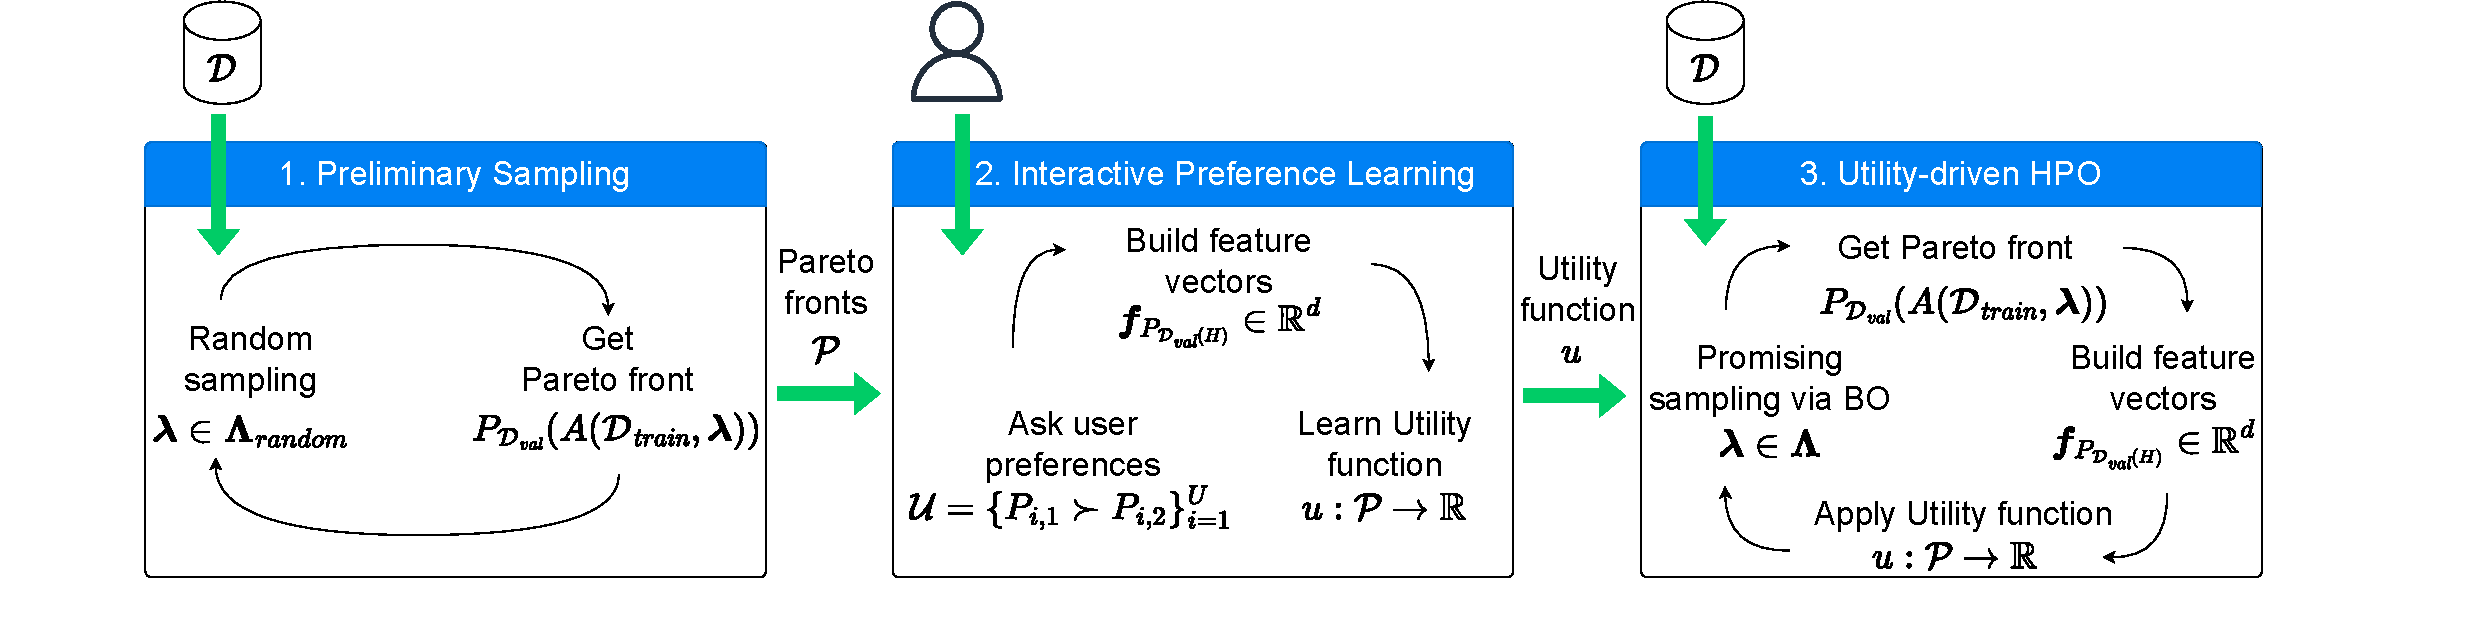
\includegraphics[width=1\columnwidth]{chapters/human-centric/moo/img/method.pdf} 
\caption{Overview of the three phases of our approach: Preliminary Sampling provides the user with different Pareto fronts, Interactive Preference Learning allows the user to express their preferences, finally, Utility-driven HPO guides the optimization to the user desiderata.}
\label{moo-fig:method}
\end{figure*}

\section{Interactive Hyperparameter Optimization in Multi-Objective Problems}
\label{moo-sec:method}

Our approach tackles the HPO problem (cf. \Cref{moo-eq:hpo}) for MO-ML algorithms, i.e., learning algorithms that return a Pareto front of models instead of a single model as a result of the learning process, works in three phases as depicted in \Cref{moo-fig:method}: 
\begin{enumerate}
    \item \textbf{Preliminary Sampling}: In the preliminary sampling phase we sample a fixed but small amount of hyperparameter configurations, evaluate these configurations and store the corresponding Pareto fronts of models returned by the MO-ML algorithm. 
    \item \textbf{Interactive Preference Learning}: In the interactive preference learning phase, we construct pairs of Pareto fronts from the ones obtained in the preliminary sampling phase and show these pairs to the user, who rates which of two shown Pareto fronts they prefer. Based on the pairwise preferences obtained from the user and feature representations of the Pareto fronts underlying these pairwise preferences, we learn a latent utility function, which, given a Pareto front, outputs a utility score.
    \item \textbf{Utility-driven HPO}: In this HPO phase, we instantiate an HPO tool (e.g. SMAC \cite{hutter-lion11a,lindauer-jmlr22a} as in our experiments) with the previously learned utility function as a loss function and perform standard HPO.
\end{enumerate}

\subsection{Preliminary Sampling}
\label{moo-ssec:sampling}

The underlying goal of the preliminary sampling phase is to obtain a set of Pareto fronts which we can use to construct pairs of Pareto fronts, which the user can rate in the subsequent stage. Keeping in mind, that we want to learn a utility function from the pairwise comparisons provided by the user, our set of Pareto fronts should ideally reasonably cover the space of possible Pareto fronts. This avoids potential generalization problems of the learned utility function, if it is provided with a Pareto front from a part of the Pareto front space which is very far off from any training data. 

Recall that we perform HPO and our MO-ML algorithm $A: \mathbb{D} \times \vec{\Lambda} \rightarrow 2^\altmathcal{H}$ returns different Pareto fronts of models for a given dataset $\altmathcal{D}_\mathit{train} \in \mathbb{D}$ based on different hyperparameter configurations $\vec{\lambda} \in \vec{\Lambda}$. As such, we can obtain a set of Pareto fronts of models by sampling a fixed number of hyperparameter configurations $\vec{\Lambda}_\mathit{random} \subset \vec{\Lambda}$ at random, training the algorithm instantiated with the corresponding hyperparameter configuration on the training data $\altmathcal{D}_\mathit{train}$ and evaluating it according to our loss functions $\altmathcal{L}_m$ on $\altmathcal{D}_\mathit{val}$. This leads to a set of Pareto fronts defined as
\begin{equation}
    \altmathcal{P} = \{ P_{\altmathcal{D}_\mathit{val}}(A(\altmathcal{D}_\mathit{train}, \vec{\lambda})) \vert \vec{\lambda} \in \vec{\Lambda}_\mathit{random}\} \, .
\end{equation}

As the rich literature on AutoML and HPO shows, random search leads to a good coverage of the hyperparameter configuration space \cite{bischl-dmkd23a}. However, this does not automatically entail a reasonable coverage of the corresponding Pareto front space. 

\subsection{Interactive Preference Learning}
\label{moo-ssec:preference_learning_method}

The goal underlying this phase of our approach is construct pairs of Pareto fronts to show to the user and learn a utility function of the form $u: \altmathcal{P} \rightarrow \mathbb{R}$, which, given a Pareto front, returns a utility score of the Pareto front based on the preferences obtained from the user. 

\subsubsection*{Acquiring User Preferences}

More formally, we start by constructing a set of pairs of Pareto fronts as 
\begin{equation}
    \Omega = \{ (P_1, P_2) \vert P_1,P_2 \in \altmathcal{P}, P_1 \neq P_2\} \, ,
\end{equation}
which leads to a number of pairs quadratic in the number of samples Pareto fronts. Since we do not want to overwhelm the user by showing them too many of such pairs, we can fallback to subsampling $\Omega$ to decrease the number of pairs to show to the user. However, as we show in the experimental evaluation later, we can also simply have a rather short preliminary sampling phase leading to a small number of Pareto fronts and thus also to a reasonably sized set $\Omega$ of pairs of Pareto fronts without compromising too much of the performance of our approach.
Once the user has rated for each of such pairs $(P_1, P_2) \in \Omega$ whether he prefers the Pareto front $P_1$ over $P_2$, we have an object ranking dataset of the form
\begin{equation}\label{moo-eq:object_ranking_dataset}
    \altmathcal{U} = \{ P_{i,1} \succ P_{i,2}\}_{i=1}^U \, ,
\end{equation} where, without loss of generality, we assume that the user prefers Pareto front $P_{i,1}$ over Pareto front $P_{i,2}$. 

\subsubsection*{Feature Representation of Pareto Fronts}
To learn a utility function based on the object ranking dataset defined in \Cref{moo-eq:object_ranking_dataset}, we additionally require a feature representation of a Pareto front such that the object ranking learning algorithm we employ can generalize over unseen Pareto fronts.
More precisely, we aim to encode the Pareto front $P_{\altmathcal{D}_\mathit{val}(H)}$ returned by $A$ in a $d$-dimensional feature representation $\vec{f}_{P_{\altmathcal{D}_\mathit{val}(H)}} \in \mathbb{R}^d$ as depicted in \Cref{moo-fig:preference_preparation}. To this end, we assume to have access to all models returned by $A$, i.e. $H$ including all dominated models internally learned by $A$ and that there is some order imposed on the model space $\altmathcal{H}$ and hence on $H$. We evaluate all of these models $H_b \in \altmathcal{H}$ with each loss function $\altmathcal{L}_i$ on $\altmathcal{D}_\mathit{val}$ resulting in the following matrix
\begin{equation}
    \vec{L} = \left( \begin{array}{ccc}
         \altmathcal{L}_1(H_1,\altmathcal{D}_{\mathit{val}}) & \ldots & \altmathcal{L}_M(H_1,\altmathcal{D}_{\mathit{val}}) \\
         \vdots & \ddots & \vdots \\
         \altmathcal{L}_1(H_B,\altmathcal{D}_{\mathit{val}}) & \ldots & \altmathcal{L}_M(H_B,\altmathcal{D}_{\mathit{val}}) \\
    \end{array} \right) \, ,
\end{equation}
where $B \geq \vert H \vert$ is the maximal number of models returned by $A$. If $A$ returns $B' < B$ values, we forward impute missing values for $B' + 1 \leq b \leq B' + (B - B')$ as 
\begin{equation}\label{moo-eq:replace_dominated}
    \vec{L}_{m,b} \leftarrow \altmathcal{L}_m(H_{b-1},\altmathcal{D}_{\mathit{val}}) ~ \forall 1 \leq m \leq M \, . 
\end{equation}
For each model $H_b$ we check if it is dominated by the previous model $H_{b-1}$ as defined in \Cref{moo-eq:pareto_def}. If it is dominated, its loss values in the matrix are replaced by the ones from the previous non-dominated model following \Cref{moo-eq:replace_dominated}.
At the end of this process, this matrix only contains loss values of 
models contained in the Pareto front.
Last, the matrix is flattened and standardized ($\altmathcal{N}(\cdot)$) across $\Omega$: 
\begin{equation}\label{moo-eq:feature_representation}
    \vec{f}_{P_{\altmathcal{D}_\mathit{val}(H)}} = \left[ \altmathcal{N}(\vec{L}_{1,1}), 
    \ldots, \altmathcal{N}(\vec{L}_{B,M}) \right] \, .
\end{equation}

Note that we assume the order on our models to, on one hand ensure that the replacement and imputation strategy works as described above, and on the other hand works as a positional encoding which, assuming a suitable order relation is defined, in itself contains valuable domain knowledge. For our experimental evaluation, we define an ordering based on loss values of one of the considered loss functions.

\begin{figure}
\centering
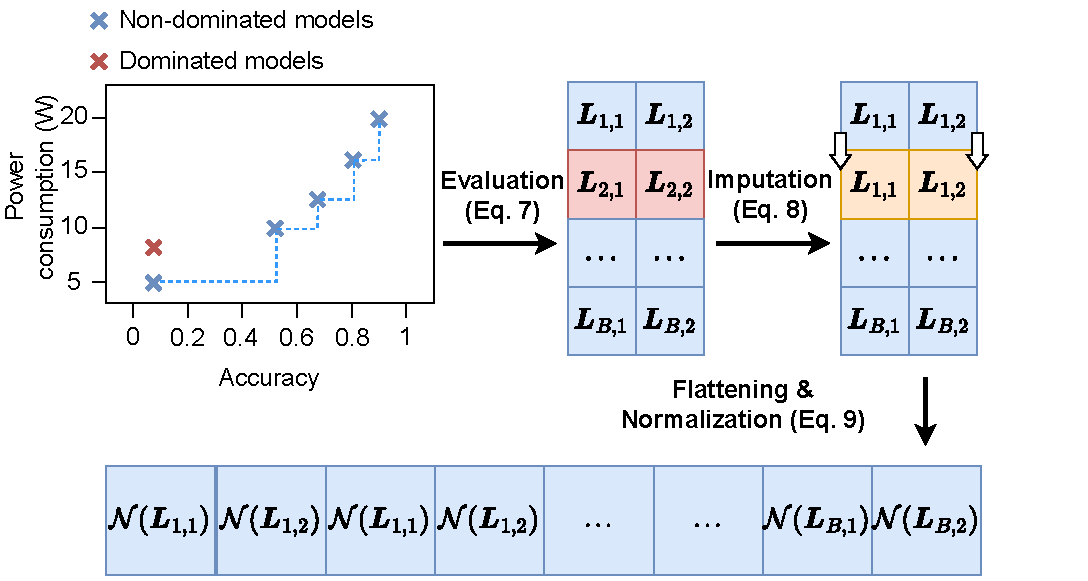
\includegraphics[width=0.7\columnwidth]{chapters/human-centric/moo/img/preference_preparation.pdf}
\caption{Visualization of the feature representation of a Pareto front based on two loss functions.}
\label{moo-fig:preference_preparation}
\end{figure}

\subsubsection*{Learning A Utility Function for Pareto Fronts}

With the object ranking dataset as defined in \Cref{moo-eq:object_ranking_dataset} and the feature representation previously described in \Cref{moo-eq:feature_representation}, we can now learn the utlity function. To this end, we leverage the RankSVM approach by \citet{joachims2002optimizing} which generalizes a standard SVM to the case of object ranking. This approach is very appealing for our use case as it allows to easily extract the latent utility function learned as part of the object ranker, which we want to use in the subsequent stage. 

The idea underlying the (linear) RankSVM is that for every pairwise comparison $P_{1} \succ P_{2}$ in our object ranking dataset $\altmathcal{U}$ we want that, without loss of generality, the hyperplane defined by the learned weight vector $\vec{w} \in \mathbb{R}^d$ separates $P_{1}$ and $P_{2}$. Formally, it should hold for every pair: % $P_{1} \succ P_{2} \in \altmathcal{U}$ that
\begin{align}
    P_{1} \succ P_{2} &\Leftrightarrow \vec{w}^\intercal\vec{f}_{P_{1}} > \vec{w}^\intercal\vec{f}_{P_{2}} \label{moo-eq:rank_svm_1} \\ 
    &\Leftrightarrow \vec{w}^\intercal\left(\vec{f}_{P_{1}}-\vec{f}_{P_{2}}\right) > 0 \label{moo-eq:rank_svm_2} \\ 
    &\Leftrightarrow \vec{w}^\intercal\left(\vec{f}_{P_{2}}-\vec{f}_{P_{1}}\right) < 0 \label{moo-eq:rank_svm_3} \, . 
\end{align}

As in the standard case of SVMs this problem is NP-hard as noted by \cite{joachims2002optimizing}, which can be solved by the standard problem relaxation leveraging slack variables as for normal SVMs. We refer to \cite{joachims2002optimizing} for details. 

With the observations formalized in \Cref{moo-eq:rank_svm_1} and \Cref{moo-eq:rank_svm_3} in mind, one can implement a RankSVM with a standard classification SVM trained with a dataset of the form 
\begin{equation}
\begin{split}
    \altmathcal{D}_{\mathit{SVM}} &= \left\{ \left(\left(\vec{f}_{P_{1}}-\vec{f}_{P_{2}}\right), 1\right) \middle\vert  P_{1} \succ P_{2} \in \altmathcal{U} \right\} \\
    &\cup \left\{ \left(\left(\vec{f}_{P_{2}}-\vec{f}_{P_{1}}\right), 0\right) \middle\vert  P_{1} \succ P_{2} \in \altmathcal{U} \right\} \, .
\end{split}
\end{equation}
We add a positive example to encourage \Cref{moo-eq:rank_svm_2} and at the same time a negative example to encourage \Cref{moo-eq:rank_svm_3}, which both enforce a balanced dataset.

After training a standard classification SVM on $\altmathcal{D}_{\mathit{SVM}}$, we define the utility function $u: \altmathcal{P} \rightarrow \mathbb{R}$ via the SVM weight vector $\vec{w}$ leveraging the feature representation of a Pareto front $P \in \altmathcal{P}$ defined in \Cref{moo-eq:feature_representation} as $u(P) = \vec{w}^T\vec{f}_P$.

Although we only explained the linear RankSVM, the kernel trick \cite{scholkopf-book02} can be applied as usual in the case of SVMs leading to non-linear versions.



All in all, preference learning and in particular object ranking offers a way to quantify the quality of a Pareto front in terms of a single scalar value w.r.t. the user desiredata without asking the user for this concrete scalar value.
The RankSVM idea leverages the robustness and effectiveness of support vector machines to operationalize this idea while offering a clear and interpretable ranking mechanism.

\subsection{Utility-driven HPO}
\label{moo-ssec:utility_automl}

As we learned the utility function $u: \altmathcal{P} \rightarrow \mathbb{R}$ from the user preferences, we want to leverage it as a Pareto front quality indicator to optimize with a standard HPO tool. To this end, we leverage the well-known HPO tool SMAC \cite{hutter-lion11a,lindauer-jmlr22a} instantiated with the learned utility function $u$ as a cost function. 


\subsection{Approach Limitations}

Naturally, our approach suffers from limitations, which we describe below together with potential remedies.

First, as we rely on showing Pareto fronts to the user, we make the implicit assumption of optimizing the hyperparameters of MO-ML algorithms which optimize only two loss functions $\altmathcal{L}_1$ and $\altmathcal{L}_2$. Although our approach would in principle also work with more loss functions, obtaining the corresponding comparison results from users would be much more complicated as showing a user a $3$-dimensional, let alone more dimensional, Pareto fronts is infeasible. A possible remedy to this problem would be to deploy dimensionality reduction techniques for multi-objectives settings \cite{deb-kangal05} such as PCA \cite{jolliffe-ftrc16}, LDA \cite{balakrishnama-article98} mapping higher dimensional Pareto fronts to two dimensions for showing them to the user.

Second, the feature representation as described in \Cref{moo-eq:feature_representation} could be improved in general to be independent of the number of loss functions. This would simplify the application of the subsequent object ranking algorithm as the replacement and imputation strategy might be discarded. On the downside, depending on the feature representation, the positional encoding, which we assume to be of importance for the learner, might get lost.

Third, 
% in Sec.~\ref{ssec:sampling}
we note that -- ideally -- the sampled Pareto fronts used to generate pairwise comparisons with the help of the user should be sampled such that the space of possible Pareto fronts is covered to avoid generalization issues of the learned utility function. However, our current approach does not actively account for this. In fact, achieving such a coverage is a challenging task as we cannot directly sample the corresponding Pareto fronts, but instead rely on sampling hyperparameter configurations leading to the Pareto front. A potential remedy for this problem could be to meta-learn a model mapping from a hyperparameter $\vec{\lambda}$ configuration to the feature vector $\vec{f}_{P_{\altmathcal{D}_{\mathit{val}}}(A(\altmathcal{D}_\mathit{train}, \vec{\lambda}))}$ representing the Pareto front obtained by running $A$ with $\lambda$. If we had such a model with a quick evaluation time, we could leverage rejection sampling and sample until we have sufficient coverage in the feature space.

Lastly, our approach is tailored towards MO-ML. However, single-objective ML is much more common in practice, limiting the applicability of our approach. As such, a generalization of our approach to doing MO-HPO of single objective ML algorithms is desirable.



\section{Empirical Evaluation}
\label{moo-sec:evaluation}

We evaluate our approach in a case-study related to decreasing the energy consumption of ML models and in particular consider an MO-ML algorithm optimizing for both accuracy and energy consumption showing how our approach can be used in the context of Green AutoML \cite{tornede-jair23a}. In the following, we first detail the general experimental setup and then present two experiments performed.

All code including detailed documentation can be found on Github\footnote{\url{https://github.com/automl/interactive-mo-ml}}, the technical appendix at the end of the document---after the references.

\subsection{General Experimental Setup}
\label{moo-ssec:experimental_setup}

The MO-ML algorithm, whose hyperparameters we want to tune, is a wrapper for a funnel-shaped artificial neural network (ANN) learning algorithm that exposes the same hyperparameters as the underlying ANN learning algorithm, but performs a grid-search over the number of epochs to train the ANN to return a Pareto front of models (\Cref{moo-fig:grid_search}).
Indeed, it is known that the \textit{number of epochs} has an obvious influence on the objectives, hence, on the shape of the retrieved Pareto front.

\begin{figure}[h]
    \centering
    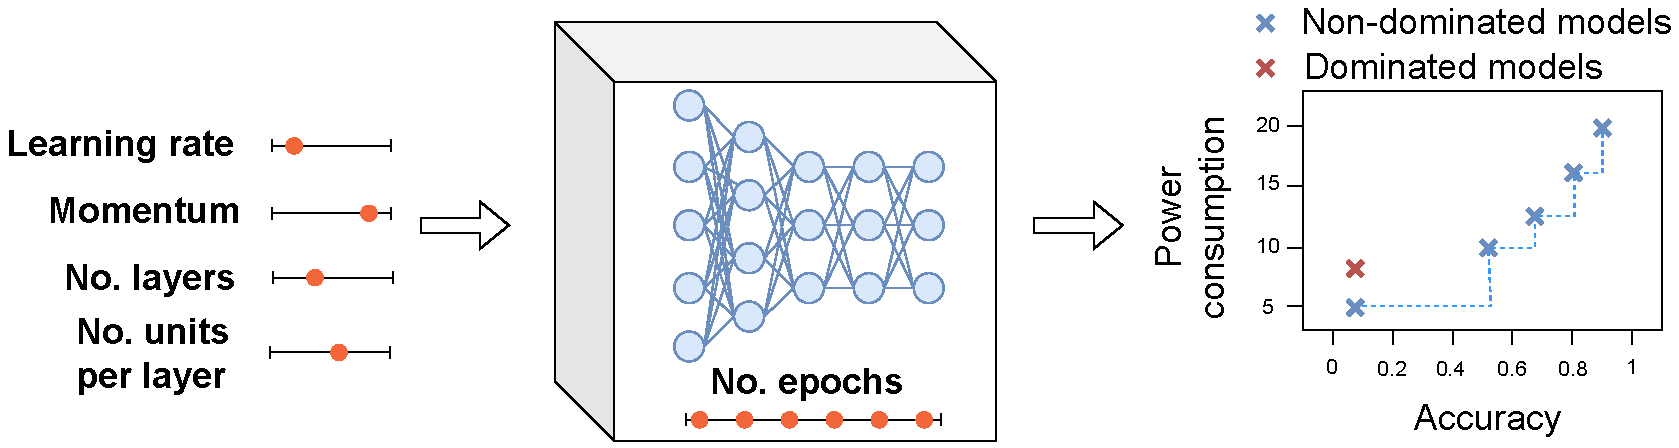
\includegraphics[width=0.8\columnwidth]{chapters/human-centric/moo/img/grid_search.pdf}
    \caption{Working example of the ANN wrapper: the grid search over the number of epochs allows us to have a Pareto front as output.}
    \label{moo-fig:grid_search}
\end{figure}

These models are all identical, but trained for different number of epochs and can thus be seen as snapshots of the ANN learning curve \cite{mohr-arxiv22a} at different epochs. A lower number of epochs usually leads to a lower energy consumption, but also to a lower accuracy indicating that the two objectives are potentially conflicting. The concrete hyperparameters our ANN algorithms exposes are defined by LCBench \cite{zimmer-tpami21a}, a well-known multi-fidelity deep learning benchmark.
LCBench comprises evaluations of over 2000 funnel-shaped MLP neural networks with varying hyperparameters on 35 datasets of the OpenML CC-18 suite \cite{bischl-arxiv17a}.
The networks use SGD with cosine annealing without restarts and, overall, $7$ parameters are sampled (4 float, 3 integer).
These are reported in \Cref{moo-tbl:lc_bench_space}.
More details can be found at \url{https://github.com/automl/LCBench}.
In the spirit of Green AutoML \cite{tornede-jair23a}, we leverage the benchmark surrogate for LCBench provided by YAHPO-GYM \cite{pfisterer-arxiv21a}.\footnote{We use the surrogate model to estimate the performance of those configurations for which no result is available in LCBench.} We measure the accuracy of a model as the validation accuracy on $33\%$ of the corresponding OpenML CC-18 dataset. We estimate the power consumption in watts~($W$) for training a model by assuming the maximum consumption for the whole provided training time. The evaluations present in LCBench were performend on an Intel Xeon Gold 6242 with a maximum consumption of $150~Wh$.

\begin{table}[t]
    \centering
    \begin{tabular}{@{}llll@{}}
    \toprule
    Hyperparameter & Type & Range & Distribution \\ \midrule
    Batch size & Integer & [16, 512] & Log \\
    Learning rate & Float & [1e-4, 1e-1] & Log \\
    Momentum & Float & [0.1, 0.99] & Linear \\
    Weight decay & Float & [1e-5, 1e-1] & Linear \\
    No. layers & Integer & [1, 5] & Linear \\
    No. units per layer & Integer & [64, 1024] & Log \\
    Dropout & Float & [0.0, 1.0] & Linear \\\bottomrule
    \end{tabular}
    \caption{Search space of LCBench.}
    \label{moo-tbl:lc_bench_space}
    \end{table}


As noted earlier, many users struggle to choose a Pareto front quality indicator as a loss function for an HPO tool that yields Pareto fronts with their desired shape. Our evaluation focuses on users that are likely to make a wrong decision wrt. choosing the correct quality indicator, but can very well label pariwise comparisons of Pareto fronts according to an indicator without knowing the indicator itself.
As such, we simulate users by labeling pairwise comparisons according to hypervolume (HV), spacing (SP), maximum spread (MS) and R2 as Pareto front quality indicators.

\begin{definition}[Hypervolume (HV)]
    Hypervolume quantifies the volume of the front by merging the hypercubes determined by each of its solutions $H \in \altmathcal{H}$ and the reference point $r$ (i.e., the worst possible solution), formally:
     $$HV(\altmathcal{H}) = \beta \left(\bigcup_{H \in \altmathcal{H}} \{ x \mid h \prec x \prec r \} \right)$$
     where $\beta$ denotes the Lebesgue measure. This ranges from $0$ to $1$, the highest the better.
\end{definition}

\begin{definition}[Spacing (SP)]
    Spacing is the most popular uniformity indicator and it gauges the variation of the distance between solutions in a set;
    $$SP(\altmathcal{H}) = \sqrt{\frac{1}{N-1} \sum_{H \in \altmathcal{H}} ( \bar{d} - d_1 ( \altmathcal{H}, \altmathcal{H}/H ) )^2}$$
    where $\bar{d}$ is the mean of all the $d_1 ( H, \altmathcal{H}/H ) : H \in \altmathcal{H}$ and $d_1 ( H, \altmathcal{H}/H )$ means the $L^1$ norm distance (Manhattan distance) of $H$ to the set $\altmathcal{H}/H$. A SP value of zero indicates all members of the solution set are spaced equidistantly on the basis of Manhattan distance.
\end{definition}

\begin{definition}[Maximum Spread (MS)]
    Maximum Spread is a widely used spread indicator, and it measures the range of a solution set by considering the maximum extent on each objective:
    $$MS(\altmathcal{H}) = \sqrt{ \sum_{j = 1}^{m} \max_{H, H' \in \altmathcal{H}} (\altmathcal{L}_{j}(H) - \altmathcal{L}_{j}(H'))^2}$$
    where $m$ denotes the number of objectives. MS is to be maximized; the higher the value, the better the extensity to be claimed.
\end{definition}

\begin{definition}[R2]
    This indicator measures the proximity to a specific reference point $r$ via the Chebyshev norm:
     $$R2(\altmathcal{H}) = \min_{H \in \altmathcal{H}} d_{\inf}(H, r)$$
     Given $m$ objectives, $d_{\inf}(H, r)$ corresponds to $\max_{i=1}^{m}(\mid \altmathcal{L}_i(H) - \altmathcal{L}_i(r))$. Lower values translate into Pareto fronts closer to the reference point, taken as the ideal solution.
\end{definition}

The order over the models returned by $A$, which we assume for the feature representation, is given by the energy consumption loss function, which means that models are ordered based on their energy consumption.

All code and documentation required to reproduce any of the results can be found on GitHub\footnote{\url{https://github.com/automl/interactive-mo-ml}}.
There is no need for the user to locally build the project, we deployed a Docker Image that instantiates a pre-built container with all the needed Python dependencies and runs the experiments.
In particular, we leverage: the package cs-rank \cite{csrank2018, csrank2019} as a basis for our preference learning models and the package pymoo\cite{pymoo} for the quality indicator implementations.
Finally, we exploit the well-known HPO tool SMAC \cite{hutter-lion11a,lindauer-jmlr22a} to apply Bayesian optimization.
The experiments were tested varying three different seeds on an AMD Ryzen $5$ $3600$ $6$-Core Processor with $64$ GB.
The total computation time was $21984$ seconds (around $6$ hours), for an overall power consumption of $520~W$.

\subsection{Object Ranking Performance}

\begin{figure}[t]
\centering
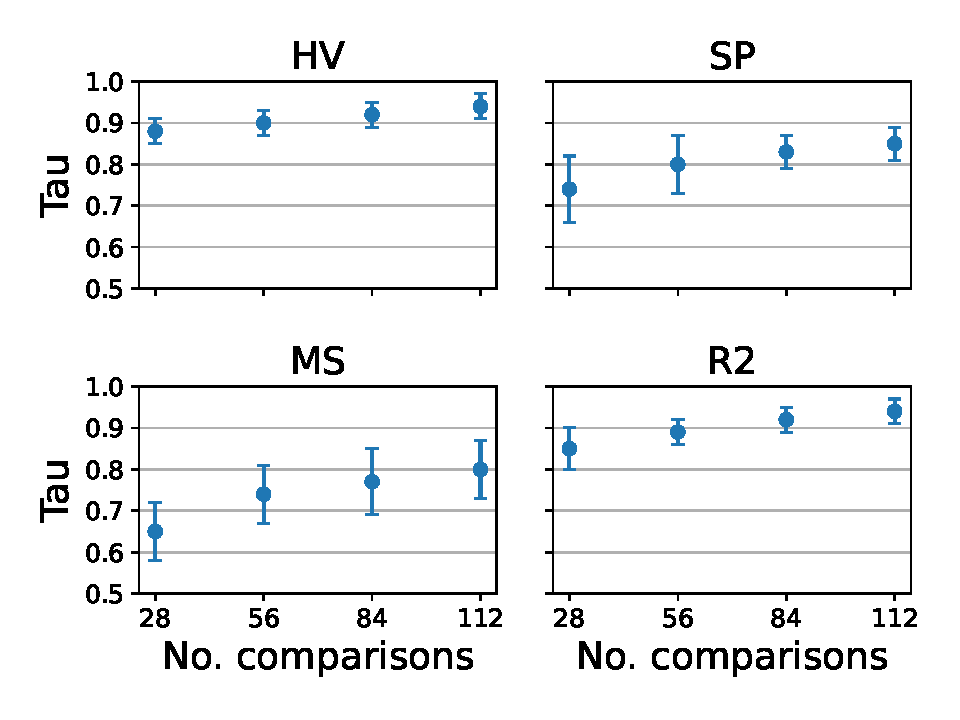
\includegraphics[width=0.7\columnwidth]{chapters/human-centric/moo/img/preference_evaluation.pdf}
\caption{Kendall's Tau of the preference learning models.}
\label{moo-fig:preference_evaluation}
\end{figure}

In the following, we evaluate our object ranker.

\paragraph{Additional Experimental Setup}
We tune the hyperparameters of our preference learning models, one for each quality indicator, on top of the first 3 datasets of LCBench: KDDCup09\_appetency, covertype, Amazon\_employee\_access.
Each configuration has been evaluated by averaging the performance achieved in those datasets over $3$ different seeds.
As to the evaluation within each dataset, we performed a cross-validation: we split the sampled Pareto fronts $\altmathcal{P}$ in $5$ folds and compute all possible pairwise comparisons within each fold. 
Specifically, we set the number of sampled Pareto fronts $|\altmathcal{P}|$ at $40$, so that we can create $5$ folds of $8$ elements, which translates into $\binom{8}{2} = 28$ pairwise comparisons.
Concretely, at each cross-validation evaluation, we use the pairwise comparisons of the $4$ training folds to predict the global ranking of the $8$ Pareto fronts in the test fold, and compare it with the ranking of the Pareto fronts given by the quality indicator at hand.
These rankings are compared in terms of a ranking loss function called Kendall's Tau correlation \cite{kendall-article48}.
Roughly speaking, this measures how correlated two rankings are. A correlation score of -1 can be interpreted as an inverse correlation, a score of $0$ as no correlation and a score of $1$ as perfect correlation.

\begin{definition}[Kendall's Tau \cite{kendall-article48}]
    Given two rankings, each position is labeled as: \texttt{concordant} $C$ if the same object is present in both rankings; \texttt{tie} $T$  if the objects are different, yet similar wrt. a certain similarity function; \texttt{discordant} $D$  if the objects are different and not similar.
    \begin{equation*}
        \textit{Tau} = \frac{(C - D)}{(C + D + T) \cdot \sqrt{C + D + T}}
    \end{equation*}
\end{definition}

To detect whether two objects -- Paretos in our case -- are similar, we employed the Fisher-Jenks algorithm \cite{fisher1958homogeneity, jenks1967data}
The Fisher-Jenks algorithm addresses the problem of determining the best arrangement of ordered values into different buckets, also known as \textit{natural breaks optimization} because it effectively highlights significant transitions in the underlying distribution.
We leverage this algorithm to identify similar Pareto fronts in the set of the Preliminary sampling, i.e., that should be ranked equally in a global ranking. The process starts by trying to divide the samples into two groups, evaluating all possible break points by the Jenks optimization function. This is the core of the algorithm because it drives towards the optimal buckets and consists of a trade-off between minimizing within-bucket variance and maximizing between-bucket variance.
Once the optimal breakpoint is found, the data is divided into two groups based on this breakpoint.
The process is then repeated recursively for each of these groups until a predetermined number of buckets is reached. By exploiting a simple elbow method, it is possible to determine the optimal number of buckets, i.e., choosing the ``knee of a curve'' as a cutoff point, where diminishing returns are no longer worth the additional cost.
Given $n$ samples to split into $k$ buckets, the complexity of the algorithm would be $O(k \cdot n^2)$. Yet, nowadays, finding breaks for $15$ classes for a data array of $7$ million unique values now takes $20$ seconds on commodity hardware. In these experiments, we have only $40$ samples to arrange in -- approximately -- $30$ buckets, depending on the indicator.


\paragraph{Result Discussion}
\begin{table}[t]
\centering
    \resizebox{0.9\textwidth}{!}{
    \Huge{
	\begin{tabular}{l|c|c|c|c}
	\toprule
	PB$\backslash$IB & $HV\uparrow$ & $SP\downarrow$ & $MS\uparrow$ & $R2\downarrow$ \\ \midrule
	$HV\uparrow$ & \cellcolor{red!1}{\begin{tabular}{ccc}  0.76  & \multirow{2}{*}{$\backslash$} & \textbf{0.77} \\ ($\pm$0.17) & & \textbf{($\pm$0.17) }\end{tabular}} & \cellcolor{blue!15}{\begin{tabular}{ccc} \textbf{ 0.76}  & \multirow{2}{*}{$\backslash$} & 0.52 \\ \textbf{($\pm$0.17)} & & ($\pm$0.24) \end{tabular}} & \cellcolor{blue!15}{\begin{tabular}{ccc} \textbf{ 0.76}  & \multirow{2}{*}{$\backslash$} & 0.52 \\ \textbf{($\pm$0.17)} & & ($\pm$0.21) \end{tabular}} & \cellcolor{red!1}{\begin{tabular}{ccc}  0.76  & \multirow{2}{*}{$\backslash$} & \textbf{0.77} \\ ($\pm$0.17) & & \textbf{($\pm$0.16) }\end{tabular}} \\ \midrule
	$SP\downarrow$ & \cellcolor{blue!67}{\begin{tabular}{ccc} \textcolor{white}{\textbf{ 0.01}}  & \multirow{2}{*}{\textcolor{white}{$\backslash$}} & \textcolor{white}{0.03} \\ \textcolor{white}{\textbf{($\pm$0.01)}} & & \textcolor{white}{($\pm$0.02)} \end{tabular}} & \cellcolor{red!0}{\begin{tabular}{ccc}  \textbf{0.01}  & \multirow{2}{*}{$\backslash$} & \textbf{0.01} \\ \textbf{($\pm$0.01)} & & \textbf{($\pm$0.0) }\end{tabular}} & \cellcolor{blue!100}{\begin{tabular}{ccc} \textcolor{white}{\textbf{ 0.01}}  & \multirow{2}{*}{\textcolor{white}{$\backslash$}} & \textcolor{white}{0.04} \\ \textcolor{white}{\textbf{($\pm$0.01)}} & & \textcolor{white}{($\pm$0.03) }\end{tabular}} & \cellcolor{blue!100}{\begin{tabular}{ccc} \textcolor{white}{\textbf{ 0.01}}  & \multirow{2}{*}{\textcolor{white}{$\backslash$}} & \textcolor{white}{0.04} \\ \textcolor{white}{\textbf{($\pm$0.01)}} & & \textcolor{white}{($\pm$0.02)} \end{tabular}} \\ \midrule
	$MS\uparrow$ & \cellcolor{blue!74}{\begin{tabular}{ccc} \textcolor{white}{\textbf{ 0.61}}  & \multirow{2}{*}{\textcolor{white}{$\backslash$}} & \textcolor{white}{0.19} \\ \textcolor{white}{\textbf{($\pm$0.09)}} & & \textcolor{white}{($\pm$0.08) }\end{tabular}} & \cellcolor{blue!74}{\begin{tabular}{ccc} \textcolor{white}{\textbf{ 0.61}}  & \multirow{2}{*}{\textcolor{white}{$\backslash$}} & \textcolor{white}{0.19} \\ \textcolor{white}{\textbf{($\pm$0.09)}} & & \textcolor{white}{($\pm$0.12) }\end{tabular}} & \cellcolor{red!6}{\begin{tabular}{ccc}  0.61  & \multirow{2}{*}{$\backslash$} & \textbf{0.65} \\ ($\pm$0.09) & & \textbf{($\pm$0.06) }\end{tabular}} & \cellcolor{blue!55}{\begin{tabular}{ccc} \textbf{ 0.61}  & \multirow{2}{*}{$\backslash$} & 0.23 \\ \textbf{($\pm$0.09)} & & ($\pm$0.11) \end{tabular}} \\ \midrule
	$R2\downarrow$ & \cellcolor{red!4}{\begin{tabular}{ccc}  0.23  & \multirow{2}{*}{$\backslash$} & \textbf{0.22} \\ ($\pm$0.16) & & \textbf{($\pm$0.16) }\end{tabular}} & \cellcolor{blue!35}{\begin{tabular}{ccc} \textbf{ 0.23}  & \multirow{2}{*}{$\backslash$} & 0.47 \\ \textbf{($\pm$0.16)} & & ($\pm$0.23) \end{tabular}} & \cellcolor{blue!32}{\begin{tabular}{ccc} \textbf{ 0.23}  & \multirow{2}{*}{$\backslash$} & 0.45 \\ \textbf{($\pm$0.16)} & & ($\pm$0.21) \end{tabular}} & \cellcolor{red!9}{\begin{tabular}{ccc}  0.23  & \multirow{2}{*}{$\backslash$} & \textbf{0.21} \\ ($\pm$0.16) & & \textbf{($\pm$0.16) }\end{tabular}} \\ \midrule
	\end{tabular}
    }
    }
\caption{Comparison between indicator-based HPO (i.e., IB, columns) and preference-based HPO (i.e., PB, rows). The preference learning model is trained using 28 pairwise comparisons.}\label{moo-tbl:end_to_end_evaluation_28}\end{table}

In \Cref{moo-fig:preference_evaluation} we plot the performance of our models in terms of the Kendall's Tau averaged across the folds with the error bars defined by the corresponding standard deviation. In particular, we show how this performance varies with the number of available pairwise comparisons, i.e. the size of the object ranking training data, highlighting that, depending on the quality indicator, we obtain a reliable ranking model for Pareto fronts with rather few training data.

Generally, as to be expected, the correlation scores increase for each utility function as the number of comparisons increases independent of the quality indicator based on which they are learned. However, both the score at the lowest number of comparisons and the degree to which it increases with a growing number of examples varies substantially between the different utility functions. This indicates that it is easier for our object ranker to learn a behavior similar to HV or R2 than to SP or MS which also coincides with the fact that HV and R2 are external quality indicators whereas SP and MS are internal indicators.
% (cf. Sec.~\ref{moo-ssec:moo}).
A potential reason for these differences in modeling performance of our object ranker might be grounded in the feature representation of Pareto fronts we chose and in the linearity of the RankSVM used as an object ranker. In particular, both SP and MS require computations over pairs of models such that a quadratic kernel or feature transformation might be better suited for these indicators. Nevertheless, as we see in the next experiment, the ranking performance seems to be sufficient to guide the HPO process.

\subsection{HPO Approach Performance}
\label{moo-sssec:end_to_end}

In the following, we leverage the remaining 32 datasets of LCBench to evaluate our complete approach from phases 1 to 3. We will demonstrate that our HPO approach performs much better than SMAC assuming a user that chooses the wrong indicator and that it performs comparable assuming an advanced user knowing which indicator to pick.

\paragraph{Additional Experimental Setup}

In order to quantify how well our approach works, we compare how well SMAC instantiated with each of the Pareto front indicators above as a loss function (IB) works compared to our approach with the user simulated as mentioned above (PB). In particular, for each Pareto front indicator, we run our approach with a simulated user that behaves according to that indicator and compare against the HPO tool instantiated with each of the indicators as a loss function. That way, we cannot only quantify how much better our approach works wrt. to each of the quality indicators, under the assumption that a user chooses a wrong quality indicator, but also that our approach does not perform substantially worse in cases where the user picks the correct indicator. We run both IB and PB for a budget of $30$ evaluations on each of the datasets for $3$ seeds and report the mean and standard deviation over the seeds and datasets.

\paragraph{Result Discussion}
\Cref{moo-tbl:end_to_end_evaluation_28} visualizes the comparison of SMAC initialized with different Pareto front quality indicators as a loss function (IB) and our approach based on the learned utility function as a Pareto front quality indicator (PB).
The indicators in the rows represent the ones used for labeling the user preferences, and hence, to train the preference learning models.
The indicators in the columns represent the quality indicators chosen for optimization in SMAC.
As a consequence, in each cell, we find the performance (averaged over seeds and datasets) and the respective standard deviation of the preference-based SMAC (PB) and the indicator-based SMAC (IB).
This is expressed in terms of the quality indicator leveraged to rank the Pareto front (i.e. the one given in the row), hence, providing us with an estimation of how compliant the final Pareto front is with the user preferences.
The cells in the diagonal correspond to situations where our approach is compared to IB initialized with the "correct" quality indicator function, whereas the off-diagonal cells correspond to scenarios where a user chooses the "wrong" quality indicato for IB. For a better visual interpretability, we color cells with a blue tone depending on how much better our approach (PB) is relative to IB given in the respective column and red in cases where we are worse. Moreover, we highlight the better performance value for each cell in bold.
If our learned utility function perfectly resembled the ground truth quality indicator, we would expect that the two values in each diagonal cell are identical and the coloring would be white as a consequence. Moreover, the better our approach is in one of the settings, the darker is the blue of the corresponding cell. At the same time, the worse our approach is in one of the settings, the darker will be the red in the corresponding cell. 

As the table shows, our approach (PB) behaves comparable to IB in cases where a user picks the correct Pareto front quality indicator (diagonal) and almost always better in cases where a user picks the wrong Pareto front quality indicator. In particular, we perform better or equal in $11/16$ cases whereas IB performs slightly better only in $5/10$ cases. In cases where our approach performs better, the improvements are often substantial, whereas in cases of degradation our approach is often only slightly worse.

Overall, our evaluation demonstrates that our approach successfully frees users from selecting the correct quality indicator aligned with their desiderata at the slight cost of visually comparing a low number of Paretos upfront.

\section{Conclusions and Fututre Works}
\label{moo-sec:conclusion}
In this chapter, we propose a human-centric interactive HPO approach tailored towards MO ML leveraging preference learning to extract desiderata from users that guide the optimization. In particular, we learn a utility function for Parto fronts based on pairwise preferences given by the user which we use as a loss function in a subsequent standard HPO process. In an experimental study, we demonstrate that our end-to-end approach performs much better than off-the-shelf HPO with a user that chooses an indicator not aligned with their desiderata and that it performs comparable to off-the-shelf HPO operated by an advanced user knowing which indicator to pick. As such, our approach successfully frees users from selecting the correct Pareto front quality indicator aligned with their desiderata at the slight cost of visually comparing a low number of Pareto fronts upfront.

As future works, we deem it interesting to design other feature representations with fewer assumptions and to generalize our approach to a larger number of loss functions as it is currently practically limited to two as users might have a hard time rating higher dimensional Pareto fronts in the interactive part.


\chapter{AutoML in the Age of Large Language Models}
\label{human-centric-chap:llm}

Large Language Models (\LLMs) \cite{zhao-arxiv23a} are currently on everybody's lips due to the recent series of rapid breakthroughs achieved, such as self-attention \cite{vaswani-neurips17a}, BERT \cite{devlin-acl19a}, several versions of GPT \cite{radford-openai18a,radford-openai19a,brown-neurips20a,openai-openai22a,openai-openai23a}, LaMDA \cite{thoppilan-arxiv22a}, LLaMA \cite{touvren-arxiv23a}, or OpenAssistant \cite{koepf-arxiv23a}. The term \LLM refers to a language model where the actual model is instantiated by a deep neural network (i.e., artificial neural networks with a large number of hidden layers) that typically features millions to billions of weights.\footnote{We note that there is no clear threshold after which a language model is called large.} Such \LLMs are pre-trained on extremely large corpora of textual datasets. Due to their excellent capabilities on various Natural Language Processing (\NLP) tasks, they have the potential to lead to the democratization of \NLP, if their pre-trained versions are accessible to the broad public and the power of \LLMs does not lay in the hand of a few companies with sufficient financial resources. Additionally,  we highlight the emerging possibilities of multimodal \LLMs~\cite{yin-arxiv2023a, wu-arxiv2023a}. By incorporating various data modalities, such as audio or images, these models enable a more flexible communication with users by capturing information presented in non-textual formats as well as facilitating the output of information in non-text formats.

Similarly, Automated Machine Learning (\AutoML) \cite{hutter-book19a} democratizes Machine Learning (\ML) by supporting data scientists in finding well-performing \ML pipelines for specific tasks through (partial) automation. \AutoML has achieved remarkable success over the last decade with heavily-used open-source frameworks such as Auto-WEKA \cite{thornton-kdd13a,kotthoff-automlbook19a}, AutoSklearn \cite{feurer-automlbook19b,feurer-jmlr22a}, AutoGluon \cite{erickson-arxiv20a}, Auto-PyTorch \cite{zimmer-tpami21a}, and closed commercialized frameworks. 

\paragraph{Motivation} With this chapter, we want to highlight our vision in which \AutoML and \LLMs are integrated with each other to radically push the boundaries of both \AutoML and \NLP. On the one hand, we expect that applying \AutoML to \LLMs improves various stages of the \LLM lifecycle by increasing their capabilities and making them more efficient. On the other hand, the disruptive \NLP and knowledge-modeling capabilities of \LLMs can unleash the full potential of \AutoML both via an integration as a human-machine-interaction component, and as a technical meta-learning component within \AutoML frameworks themselves. Correspondingly, this chpater is targeted both 
\begin{itemize}
    \item at \NLP researchers leveraging \AutoML methods to further improve \LLMs and
    \item at \AutoML researchers who seek to leverage the strengths of \LLMs to improve \AutoML paradigms and tools in various regards outlined below.
\end{itemize}
Consequently, we only sparsely mention general topics or problems concerning \LLMs, but focus on problems and aspects that arise from the intersection of the two fields.
For a more general survey on \LLMs, we refer the reader to \cite{zhao-arxiv23a}.
To make this chapter as tailored as possible, we explicitly chose not to focus on pre-trained models in general, but focus on language models as they allow extracting knowledge from the large set of unstructured data in the form of text on the web which certainly contains valuable AutoML knowledge.\footnote{We note that there also exists work in the broader intersection of \AutoML and pre-trained models \cite{hollmann-iclr23a,muller-icml23a} which is outside the scope of this chapter as we only focus on (pre-trained) \LLMs and not pre-trained models in general.}

\paragraph{Contributions} To showcase our vision, we explore the potential of a symbiotic relationship between \AutoML and \LLMs, including a survey of existing work on the matter. We start by investigating the challenges of applying \AutoML to \LLMs, in particular Neural Architecture Search (\NAS) \cite{elsken-jmlr19a,wistuba-arxiv19a,white-arxiv23a} and Hyperparameter Optimization (\HPO) \cite{feurer-automlbook19a,bischl-dmkd23a}, as well as potential solutions for optimizing pre-training, fine-tuning, and inference (\Cref{llm-sec:automl-for-llms}). Subsequently, we swap perspectives and elaborate on opportunities offered by \LLMs to improve \AutoML approaches in terms of human-machine-interaction, the configuration of \AutoML systems, and the replacement of parts of \AutoML systems by an \LLM (\Cref{llm-sec:llms-for-automl}). In order to give a balanced outlook, we also critically assess potential risks which might arise due to an integration of \AutoML and \LLMs (\Cref{llm-sec:dangers-and-challenges}). 

The main insights we want to bring across with this work are the following: 
\begin{itemize}
    \item Current \AutoML approaches are not ready for a holistic optimization of the whole lifecycle of \LLMs due to several challenges, such as the computational demand of pre-training and the multi-stage training process of \LLMs featuring varying metrics and learning paradigms. 
    \item An integration of \LLMs with \AutoML tools has the potential to substantially improve the human-machine-interaction component of corresponding tools, alleviate the tedious task of correctly configuring an \AutoML tool and to improve several internal components of \AutoML tools through knowledge gained on meta-learning from unstructured data.
    \item Integrating the two research areas with each other naturally also bears risks such as inadequate evaluation of \LLM powered \AutoML systems, catastrophically wrong behavior of \AutoML systems due to hallucinations of an \LLM powered component, (too) high trust in results of an \AutoML tool explained through natural language and ever-increasing resource demands.
\end{itemize}

%%%%%%%%%%%%%%%%%%%%%%%%%%%%%%%%%%%%%%%%%%%%%%%%%%%%%%%%%%%%%%%%%%%%%%%%%%%%%%%%%%%%%%%%%%%%%%%
%%%%%%%%%%%%%%%%%%%%%%%%%%%%%%%%%%%%%%%%%%%%%%%%%%%%%%%%%%%%%%%%%%%%%%%%%%%%%%%%%%%%%%%%%%%%%%%
\section{AutoML for \LLMs}
\label{llm-sec:automl-for-llms}
%(2 pages + figures)
%%%%%%%%%%%%%%%%%%%%%%%%%%%%%%%%%%%%%%%%%%%%%%%%%%%%%%%%%%%%%%%%%%%%%%%%%%%%%%%%%%%%%%%%%%%%%%%
%%%%%%%%%%%%%%%%%%%%%%%%%%%%%%%%%%%%%%%%%%%%%%%%%%%%%%%%%%%%%%%%%%%%%%%%%%%%%%%%%%%%%%%%%%%%%%%

One could argue that \AutoML for \LLMs is yet another application of \AutoML. However, compared to previous applications of \AutoML to different learning paradigms, \LLMs come with a complete set of new challenges, rendering the standard approaches of existing \AutoML tools partially useless. In fact, \citet{godbole-github23} argues that standard \HPO tools cannot be applied off-the-shelf for optimizing very deep and thus resource-intensive neural networks such as \LLMs. Furthermore, as pointed out by \cite{hutter-blog22a} in his vision for Deep Learning 2.0, we need to bring many ideas together and face new challenges if we want to automatically obtain models of the same or a better quality level as the ones currently manually designed for deep learning including \LLMs.

In a nutshell, we see five main challenges which need to be addressed: 
\begin{enumerate} 
    \item Pre-training the base model of \LLMs is extremely expensive such that very few full training runs -- maybe even only a single one -- of the \LLM base model are possible.
    \item The \AutoML task is complex and ideally has to be performed across many steps of the \LLM lifecycle, including pre-training, several steps for fine-tuning, and inference. However, these steps currently cannot be addressed in a single joint, holistic optimization and instead have to be performed independently most of the time;
    \item Finding good neural architectures to solve a specific problem is a tedious task and modern automated methods such as \NAS can only do so to a certain extent, but have not yet been able to produce new ground-breaking architectures.
    \item All of the stages of the \LLM lifecycle call for the optimization of a different metric. Especially in pre-training this metric can be seen to act as a proxy for the final performance across a variety of different tasks, which the \LLM could be used for. This can lead to potentially misleading, noisy, and biased performance indicators for the \AutoML process.
    \item \AutoML commonly considers only a single learning paradigm (e.g. supervised learning) at a time. However, training \LLMs is challenging as the different stages of the lifecycle require different learning paradigms.
\end{enumerate}

After providing more background on \LLMs in the next subsection, we delve into details for all these challenges and discuss existing \AutoML ideas that are either applied already to \LLMs or could be a promising future direction.

\begin{figure}
    \centering
    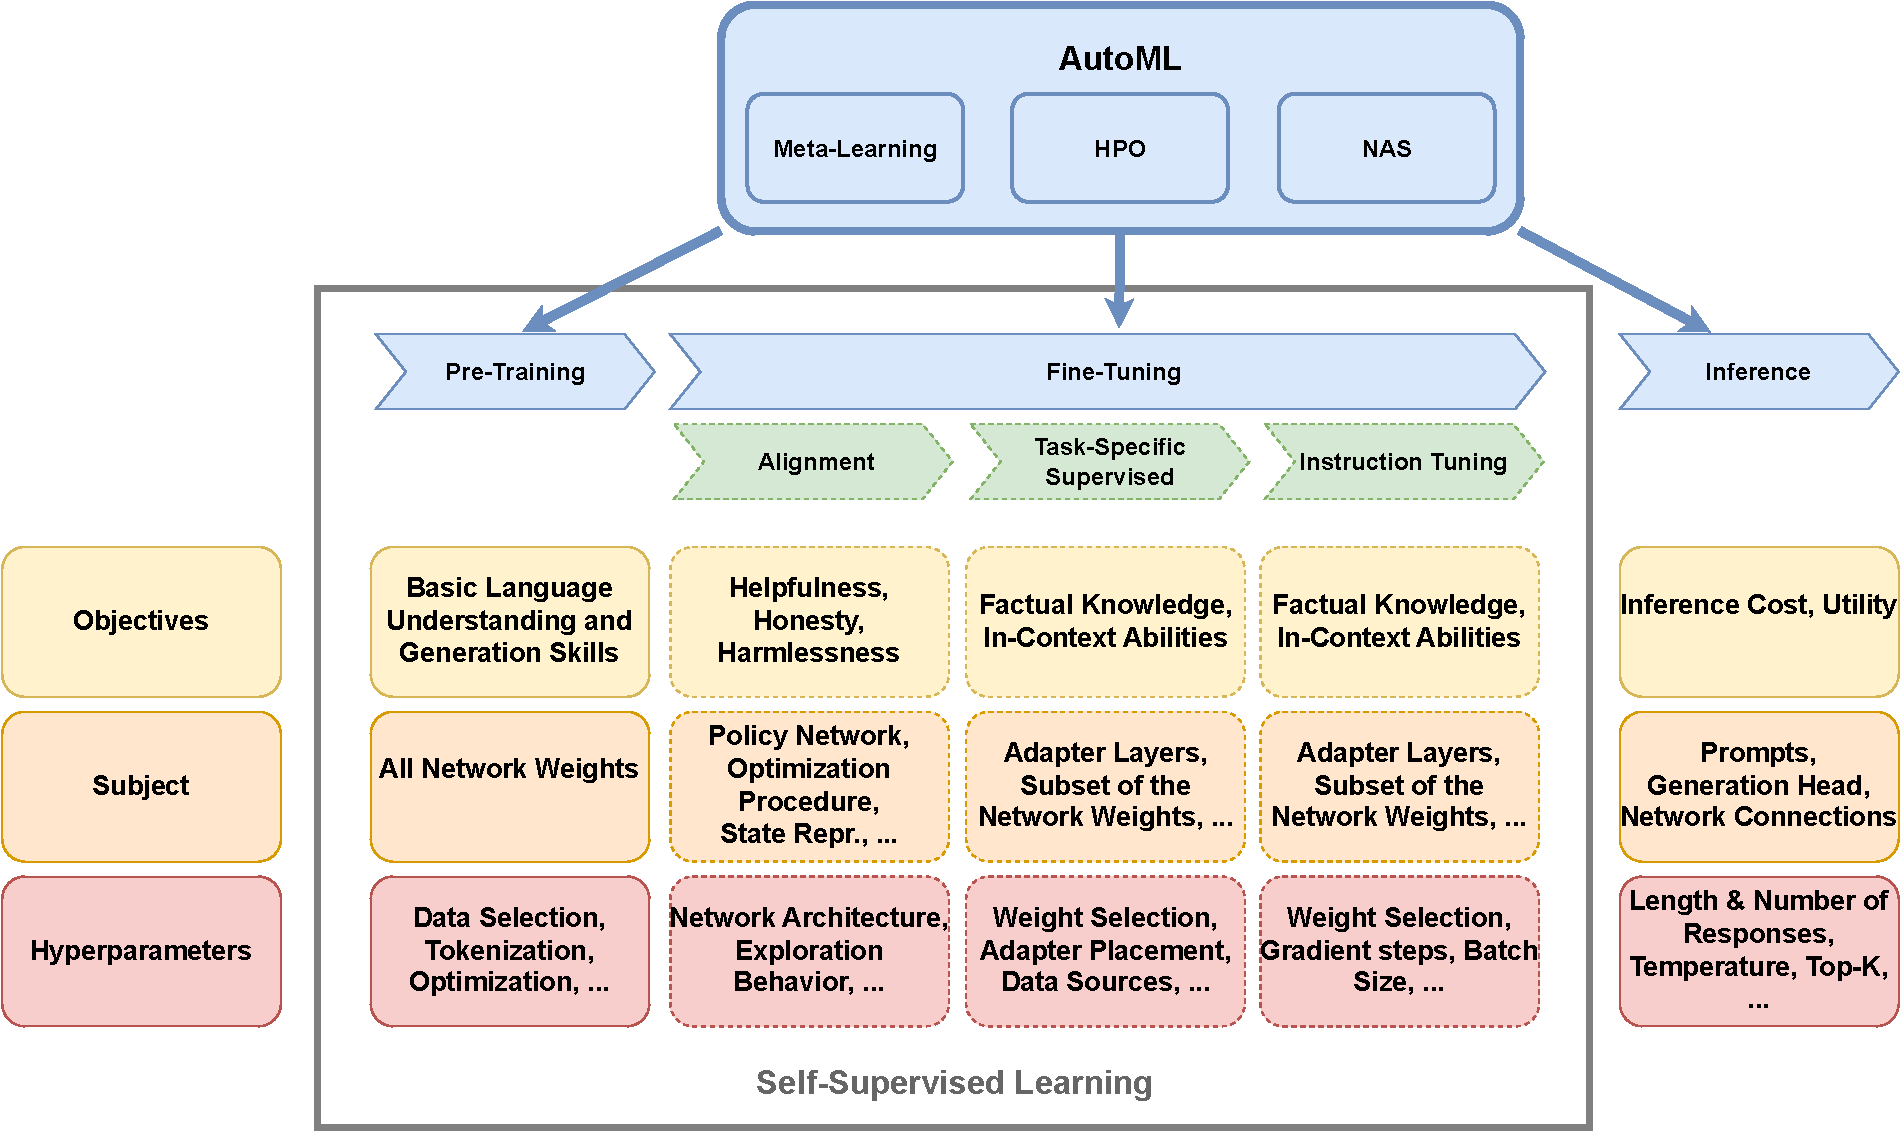
\includegraphics[width=.75\textwidth]{chapters/human-centric/llm/img/automl_for_llms.pdf}
    \caption{\AutoML can be used in all stages of the \LLM lifecycle and needs to be adjusted to the different objectives, hyperparameters, and design decisions of each stage. The graphic depicts exemplary objectives, subjects of optimization, and associated hyperparameters. Due to computational constraints, the stages are considered separately, one after the other.}
    \label{llm-fig:automl_for_llms}
\end{figure}

%%%%%%%%%%%%%%%%%%%%%%%%%%%%%%%%%%%%%%%%%%%%%%%%%%%%%%%%%%%%%%%%%%%%%%%%%%%%%%%%%%%%%%%%%%%%%%%
\subsection{Background on \LLMs}
%%%%%%%%%%%%%%%%%%%%%%%%%%%%%%%%%%%%%%%%%%%%%%%%%%%%%%%%%%%%%%%%%%%%%%%%%%%%%%%%%%%%%%%%%%%%%%%

The lifecycle of an \LLM typically involves three key stages: pre-training, fine-tuning, and inference \cite{zhao-arxiv23a}. Each stage of this lifecycle comes with its own set of objectives, hyperparameters, and design decisions affecting the final performance on downstream tasks, as depicted in \autoref{llm-fig:automl_for_llms}.

During \textbf{pre-training}, the base model is trained on a large corpus of unlabeled text to learn language patterns and capture general knowledge about the language. The overall goal of pre-training is to produce useful representations of sequences with a pre-text task in a quasi-unsupervised fashion which corresponds to the first stage of the Self-Supervised Learning (SSL) paradigm \cite{balestriero-arxiv23a}. 
It is typically the most expensive part of training an \LLM and only a few groups and companies world-wide can afford to pre-train a base model.

\textbf{Fine-tuning} follows, where the pre-trained model is further trained on domain- or task-specific data to specialize its knowledge and adapt to specific tasks,  domains, or use cases. In general, fine-tuning covers various groups of approaches such as task-specific supervised fine-tuning \cite{zhao-arxiv23a}, instruction tuning \cite{wei-iclr22a}, and alignment fine-tuning \cite{zhao-arxiv23a}. 
The success in this specialization is quantified with a corresponding metric or loss function. 
Provided the pre-training found useful representations, the objective here is to utilize or adapt these representations with specific downstream tasks in mind.
This can be very effective even with limited data for the downstream task and thus is computationally much less demanding than training a base model.
The probable reason is that for a given downstream task, there often exists a low-dimensional reparametrization of the strong joint embedding which was learned during pre-training featuring a large number of parameters. This allows to unleash the full power of transfer learning \cite{aghajanyan-acl21}.

Instruction tuning can be seen as generalized task-specific supervised fine-tuning that teaches LLMs to follow instructions in the form of prompts.
It fine-tunes a single model using instructions via prompts that span various tasks, thereby enabling the prompting of LLMs. A very specific and, from an \AutoML perspective, complicated task that is often solved by a form of instruction tuning, called Reinforcement Learning from Human Feedback (RLHF)~\cite{fernandes-arxiv23a}, is alignment.%
\footnote{We note that there are recent approaches aimed at replacing reinforcement learning with supervised approaches such as classification losses~\cite{rafailov-arxiv23a}. Moreover, in general instruction tuning covers a large range of techniques such as self-instruct \cite{wang-acl23a}.}
Alignment (fine-tuning) describes the idea of approximately aligning the behavior and output of \LLMs with human value-related task objectives such as helpfulness, honesty, harmlessness, etc.
The two ingredients required to make Reinforcement Learning (RL) work on a pre-trained Language Model (\LM) are:
\begin{itemize}
    \item A Reward Model (RM) to convert a sequence of texts to a scalar reward which numerically represents the human preference.
    \item A policy that takes user queries or prompts as input to produce language tokens as outputs.
\end{itemize}

We note that, in principle, one can also use a pre-trained model off-the-shelf. However, in practice, some instruction tuning and alignment fine-tuning is performed if the model is released to end-users. Moreover, some form of additional task-specific fine-tuning is often performed to increase the performance of the \LLM for its designated usage and to make it properly usable.

Finally, during \textbf{inference}, the fine-tuned \LLM generates text for language-related tasks, such as question answering, based on the learned knowledge and contextual understanding.

%%%%%%%%%%%%%%%%%%%%%%%%%%%%%%%%%%%%%%%%%%%%%%%%%%%%%%%%%%%%%%%%%%%%%%%%%%%%%%%%%%%%%%%%%%%%%%%
\subsection{Challenge I: Cost of Pre-Training Base Models}
%%%%%%%%%%%%%%%%%%%%%%%%%%%%%%%%%%%%%%%%%%%%%%%%%%%%%%%%%%%%%%%%%%%%%%%%%%%%%%%%%%%%%%%%%%%%%%%

Applying standard black-box \AutoML approaches, such as grid search, random search, bayesian optimization or evolutionary algorithms, to pre-train \LLMs is simply not feasible since a single pre-training of an \LLM requires hundreds of GPUs for days. \cite{brown-neurips20a} estimate that a single training of GPT-3 required months on a thousand V100 GPUs. To put it in numbers, consider tuning $10$ hyperparameters and that a black-box AutoML optimizer requires at least $10$ times the number of hyperparameters as samples \footnote{We note that some optimizers recommend $10$ times the number of hyperparameters as samples alone for the initial design before the actual optimization starts.}, we would need $100$ months (i.e., more than 8 years) on a thousand V100 GPUs. Even when considering smaller and potentially open-source \LLMs, many still require training on a considerable amount of compute units (be it GPUs or TPUs) for several days, yielding training resource requirements of hundreds of exaFLOPS \cite{geiping-icml23a} just for a single training run. Since emerging abilities of \LLMs only happen from a certain size onward, size is important and thus, large training costs are often unavoidable. In view of recent state-of-the-art approaches to \AutoML, there could be two ways to address this, as discussed in the following.

\subsubsection{Prior-Guided Multi-Fidelity Optimization with Scaling Laws}

In cases where many full training evaluations with different hyperparameters or neural architectures are not feasible, a common \AutoML approach is multi-fidelity optimization. The general idea is to approximate the real target function by a less expensive fidelity (e.g., by training for fewer epochs or by training on less data) making this a natural candidate strategy for \HPO for \LLMs.

However, even multi-fidelity approaches require at least tenths of full training runs to perform well. At the same time, human experts are somewhat successful in tuning \LLMs manually without excessive re-trainings. Guided by this observation on earlier \AutoML problems, the community developed approaches leveraging intuitive prior knowledge of experts. While \cite{souza-ecmlpkdd21a} and \cite{hvarfner-iclr22a} proposed ways to integrate prior knowledge on the location of promising hyperparameter configurations into bayesian optimization, \cite{mallik-neurips23a} extended this idea to multi-fidelity optimization and achieved strong performance within ten full training runs.

Moreover, multi-fidelity approaches have to be configured correctly, in particular regarding the choice of the fidelity type, to achieve strong performance. This choice should be based on the observation that the ordering among potential configurations on low-fidelity approximations should be correlated with the maximum fidelity. It is currently unclear, if such an assumption can be made for \LLMs considering recent work, e.g., by \citet{kirsch-arxiv22a}.
Even more related, in the pursuit of understanding the interplay between the size of a language model and its performance, recent works have delved into the scaling laws of language models \cite{radford-openai19a, brown-neurips20a, kaplan-arxiv2020a}. 
They showed that improvements along scale dimensions generally lead to an increase in performance, both for parameter scaling dimensions such as the network width and depth, computational scaling dimensions such as the number of training steps, and the amount of data used for training.
When not limited by the other two factors, performance exhibits a power-law correlation with each of the three scale factors, bounded by diminishing returns. Correspondingly, under reasonable assumptions, multi-fidelity approaches seem to be indeed very suitable, if correctly configured.

Motivated by the same idea of leveraging cheap approximations, \citet{yang-neurips21a} mitigate the large cost of \LLM hyperparameter optimization by leveraging specific network parametrizations that allow for stable training across model sizes. 
This way, a smaller version of the actual model can be tuned, and the best-found hyperparameter configuration can be transferred to the larger model. 
However, the approach is limited to hyperparameters that have a stable optimum across different network scales under the network parameterization. 
Naturally, this excludes hyperparameters that define the training scale, which other hyperparameters are transferred across.
As shown in the paper, hyperparameters with a strong regularization effect, such as dropout probability and weight decay, were empirically found not to transfer well.

%%%%%%%%%%%%%%%%%%%%%%%%%%%%%%%%%%%%%%%%%%%%%%%%%%%%%%%%%%%%%%%%%%%%%%%%%%%%%%%%%%%%%%%%%%%%%%%
\subsubsection{Gradient-Based \AutoML}

Instead of having an outer loop training an \ML model with different configurations over and over again, it would be desirable to learn the hyperparameters on the fly while training the \ML model. This would be specifically interesting for \LLMs when we can afford only one training run. Although gradient-based optimization is possible both for \HPO~\cite{maclaurin-icml15a,luketina-icml16a,franceschi-icml17a,mackay-iclr19a,lorraine-aistats20a} and neural architecture search w.r.t. individual cells of the network~\cite{liu-iclr19a,elsken-jmlr19a}, these approaches struggle so far with robustness and scaling to large networks such as \LLMs.

%%%%%%%%%%%%%%%%%%%%%%%%%%%%%%%%%%%%%%%%%%%%%%%%%%%%%%%%%%%%%%%%%%%%%%%%%%%%%%%%%%%%%%%%%%%%%%%
\subsubsection{Meta-Learning When and How to Adjust Training}

If we think about how human experts train \LLMs, they use check-pointing s.t. they can intervene if the training threatens to fail, e.g., changing the learning rate accordingly. Overall, this manual strategy resembles dynamic configuration approaches~\cite{adriaensen-jair22a} that meta-learn how to adjust the hyperparameter configurations while the training of the model is ongoing. 
Going even one step further would lead to learning the learning process itself~\cite{andrychowicz-neurips16a,chen-neurips22a}.
Since this approach requires an offline meta-learning for obtaining the corresponding meta-policy (e.g., learned with RL), it is an open problem how to scale it up to \LLMs where the collection of meta-learning and evaluations of the meta-policy is not trivially feasible.


%%%%%%%%%%%%%%%%%%%%%%%%%%%%%%%%%%%%%%%%%%%%%%%%%%%%%%%%%%%%%%%%%%%%%%%%%%%%%%%%%%%%%%%%%%%%%%%
\subsection{Challenge II: A Multitude of Different Stages}
%%%%%%%%%%%%%%%%%%%%%%%%%%%%%%%%%%%%%%%%%%%%%%%%%%%%%%%%%%%%%%%%%%%%%%%%%%%%%%%%%%%%%%%%%%%%%%%


As we illustrate in Figure~\ref{llm-fig:automl_for_llms}, the \LLM lifecycle comprises different stages and each of them has different objectives, subjects and hyperparameters. That makes a holistic \AutoML approach very hard and, perhaps, even impossible. Although it is in principle possible to tune complex pipelines of predictive models~\cite{wachsmuth-cicl13a,feurer-nips15a,wever-automl18a,olson-automl19a}, it would be too expensive to tune all stages of the \LLM training jointly. Moreover, they even do not follow the same metrics for the objectives. Therefore, we usually tune them independently and discuss them step by step in the following.

%%%%%%%%%%%%%%%%%%%%%%%%%%%%%%%%%%%%%%%%%%%%%%%%%%%%%%%%%%%%%%%%%%%%%%%%%%%%%%%%%%%%%%%%%%%%%%%
\subsubsection{Pre-Training}

Hyperparameter Optimization for pre-training is not only expensive, as previously discussed, but also spans a variety of very different types of hyperparameters.  
Selecting data sources for pre-training is a subtle but crucial choice to this end. 
It affects the domain-specific and general knowledge encoded into the \LLM, while also impacting its conversational and reasoning abilities \cite{zhao-arxiv23a}.
Additionally, data pre-processing decisions impact the data quality and, in turn, affect the downstream performance. 
As with all text-based models, tokenization \cite{schuster-ieee2012, sennrich-acl2016a, kudo-acl2018a} plays a key role in the training data representation.
Subsequently, the intricacies of the backbone architecture of the \LLM must be decided. 
Transformer-based models \cite{vaswani-neurips17a} are the avant-garde in language models.
Designing such a transformer model comprises several crucial architectural choices such as a range of different encoder-decoder architectures \cite{vaswani-neurips17a, lewis-acl20a}, decoder architectures \cite{brown-neurips20a, zhang-arxiv2022a} and encoder architectures \cite{devlin-acl19a,liu-arxiv19a}.
Similarly, a key configuration option is the choice of self-supervised training strategies \cite{lewis-acl20a}. Besides, choices regarding normalization \cite{ba-arxiv2016a, xiong-icml20a}, activation functions \cite{hendrycks-arxiv2016a, shazeer-arxiv2020a}, or positional encoding \cite{su-arxiv2022}, as well as training settings such as the optimizer \cite{kingma-iclr15a, loshchilov-iclr18a, shazeer-icml18a}, learning rate schedule~\cite{loshchilov-iclr17a}, and batch size have to be made. 

%%%%%%%%%%%%%%%%%%%%%%%%%%%%%%%%%%%%%%%%%%%%%%%%%%%%%%%%%%%%%%%%%%%%%%%%%%%%%%%%%%%%%%%%%%%%%%%
\subsubsection{Fine-Tuning}
As fine-tuning approaches can be categorized into groups following different learning paradigms, corresponding challenges also differ according to the learning paradigm as we outline below.



\paragraph{Supervised Task-Specific Fine-Tuning} Task-specific fine-tuning can be regarded a standard supervised-learning stage based on input-output pairs (with or without instructions). That is,
\LLMs can still be fine-tuned to specific tasks without instruction tuning, and since the realization of the two is different, the application of AutoML differs in practice. AutoML for supervised fine-tuning in principle could follow the same approaches as extensively studied in the AutoML community since it provides a clear supervised training signal and is feasible computation-wise. Interesting questions arise with respect to neural architecture search to which we will come back later. One of the core challenges associated with supervised (task-specific) fine-tuning is that it can undo some of the alignment achieved via alignment fine-tuning \cite{qi-arxiv23a} such that the two stages are ideally considered jointly when performing \HPO.

\paragraph{Instruction Tuning}

With instruction tuning being a specific type of generalized supervised task-specific fine-tuning \cite{wei-iclr22a} that prepares LLMs for prompting, similar challenges as for supervised task-specific fine-tuning arise when performing \AutoML for this stage.
In particular, this is the case since instruction tuning is also a form of supervised fine-tuning generalized to multiple tasks and thus, \AutoML approaches for supervised learning can be used.
While optimizing instruction tuning using AutoML boils down to the techniques already available for supervised learning problems, a few additional challenges arise.

First, curating the necessary task-specific data in sufficient quality and quantity is cumbersome and potentially labor-intensive.
To alleviate the burdensome quantity issue, trained LLMs can be prompted using templates as a data extraction module ~\cite{zhang-arxiv23c}.
The quality of the extracted dataset, however, adheres to prompt engineering and LLM inference hyperparameters located in the pre-processing pipeline.
They can be subjected to \AutoML methods.

Second, oftentimes tasks share an inherent structure or knowledge as in coding tasks for code summarization or code completion.
Exploiting the similarities using multi-task learning can facilitate improved (generalization) performance, robustness, data efficiency and data imbalance across tasks \cite{liu-arxiv23a}.
With the ability to generate ample datasets and related tasks at arguably significant cost, task selection may become an issue.
\cite{kung-emnlp23a} resort to active learning in order to solve it, but \AutoML could also be invoked to assist in this selection. 


A third challenge arises from the multi-task nature of the tuning process as the cost function optimized by an \AutoML approach has to be able to capture the performance across multiple tasks.
While this problem is prevalent in the related field of algorithm configuration~\cite{schede-jair22a}, it is less so in \AutoML.
Nevertheless, corresponding approaches exist \cite{perrone-neurips18a,law-neurips19a,li-kdd22a}.
In general, \AutoML can help with finding the right hyperparameter values for instruction tuning that are described by \citet{wei-iclr22a} such as the number of gradient steps, the batch size, the optimizer or the learning rate.

\paragraph{Alignment Fine-Tuning}
% \AutoML for Reward Model ad Policy networks
Alignment fine-tuning is usually performed via reinforcement learning, more precisely RLHF~\cite{fernandes-arxiv23a}. Although RLHF can be seen as a form of instruction tuning, we dedicate a separate paragraph to alignment tuning and RLHF here, as they are complicated problems from an \AutoML perspective due to their dependability on reinforcement learning \cite{eimer-icml23a}.\footnote{We note that there are recent approaches aimed at replacing reinforcement learning with supervised approaches, such as classification losses~\cite{rafailov-arxiv23a}.}
Unfortunately, RL is not well studied from an \AutoML perspective.
There are still many open questions, such as properties of hyperparameter landscapes in RL~\cite{mohan-automlconf23a}, sound evaluation protocols~\cite{eimer-icml23a}, stability of training due to the non-stationary learning task and non-deterministic data collection on the fly, especially in online and on-policy learning.
The nonstationarity in the training data introduces noise to the performance observations for \AutoML systems and increases the risk of overfitting the tuning process to a few random seeds~\cite{eimer-icml23a}.

Automated Reinforcement Learning (AutoRL)~\cite{parkerholder-jair22a} aims to address these issues through techniques such as hyperparameter optimization for RL~\cite{li-kdd19a,parkerholder-neurips20a,wan-automl22a}, learned optimizers~\cite{lan-arxiv23a}, neural architecture search~\cite{wan-automl22a} and dynamic configurations~\cite{adriaensen-jair22a}.
Most of these considerations of AutoRL translate to the RL components of \LLMs; thus, corresponding methods might be a suitable choice.
However, at the current point in time, appropriate tuning of RL for \LLM is even more understudied than AutoRL for traditional RL benchmarks such as control or games.

A crucial design decision is the RL algorithm itself. PPO~\cite{schulman-arxiv17a} and A2C~\cite{mnih-icml16a} are currently common choices for RLHF.
However, in principle, the scalar nature of the reward in the RL optimization stage of \LLM alignment allows seamless integration of many existing RL algorithms.
Thus, selecting RL algorithms based on the task at hand could leverage further potential here~\cite{laroche-iclr18a}.


Most RLHF-specific design decisions related to the reward model (RM) are not used in standard RL and thus are not studied in the existing AutoRL literature.
A crucial design decision for the RM is determining its size relative to the pre-trained \LLM.
There is no established standard for this, with current solutions being driven heuristically.
For example, OpenAI uses an RM with 6 billion parameters for an \LLM with 175 billion parameters, while Deepmind uses the same size for both the RM and the \LLM~\cite{lambert-hf22a}.
This design decision could depend on the downstream task for which the fine-tuning is being performed and the multiple objectives the preference score aims to capture.
Optimizing for optimal size ratio for RM with respect to the \LLM is a configuration problem that could be sped up via learning-curve-based multi-fidelity methods~\cite{klein-iclr17a,jawed-ecml21a,ruhkopf-tmlr23a}.
Recent results on the positive impact of incorporating multiple reward models to produce a more expressive reward signal~\cite{wu-arxiv23a} open up new avenues for methods that can utilize ensembling methodologies for task-specific fine-tuning architectures.
Moreover, methods to iteratively update the RM and policy together~\cite{lambert-hf22a,bai-arxiv22a} could open the doors to complex dynamics for which AutoRL hyperparameter landscapes~\cite{mohan-automlconf23a} can be utilized for designing better optimizers and multi-fidelity methods.

Another departure from standard AutoRL is the policy update in RLHF, which is usually performed only on a subset of the weights due to the size of the \LLM~\cite{hu-iclr22a,glaese-arxiv22a}. 
This subset of weights for the update depends on multiple factors, including the complexity of concepts in the data, preference scores, and the size of the \LLM.
Methods for data generation through exploration and curriculum learning to adaptively select the best data for the policy update can serve particularly useful in this scenario~\cite{jiang-arxiv23}.
Techniques from multi-objective optimization could be further used to balance data quality, policy updates and number of parameters to update. 


%%%%%%%%%%%%%%%%%%%%%%%%%%%%%%%%%%%%%%%%%%%%%%%%%%%%%%%%%%%%%%%%%%%%%%%%%%%%%%%%%%%%%%%%%%%%%%%
\subsubsection{Inference}

Inference queries imply forward passes through billion-parameter models, leading to high deployment costs that can be computationally as well as ecologically costly. 
The former is particularly important since a multitude of \LLMs fine-tuned to a variety of tasks serve large communities of users.
As a consequence, mitigating these costs and maximizing the utility for the users should be the prime objective of this stage and results in a difficult multi-objective optimization problem.
% Mixed precision training \cite{shen-aaai2020a, dettmers-arxiv2022a} and automated pruning techniques \cite{chen-ijcai20, wang-emnlp20a} can help to reduce this cost. 
Automated pruning techniques \cite{chen-ijcai20, wang-emnlp20a} can help to reduce this cost. In addition, mixed precision \cite{shen-aaai2020a, dettmers-arxiv2022a}, which uses 16 bits (or even less) and 32 bits to represent floating point numbers, reduces memory usage and accelerates computations in training as well as inference~\cite{Yuan-air23a}.
Similarly, adjusting the maximum number of generated tokens, i.e., the length of a response or the number of responses, in cases where the user asks for multiple ones, can help to reduce the cost but might harm the user benefit.
Moreover, tuning hyperparameters that affect the randomness of the generated text, such as temperature or top-k adjustments, may increase the utility but naturally can impact the expected number of queries needed to achieve a desired output. 
Notably, advanced decoding strategies \cite{zhao-arxiv23a} including repeated prompting and templates or chain-of-thought related concepts \cite{besta-arxiv23a,ning-arxi23a} may provide noticeable improvements. However, automatically optimizing inference via means of \AutoML is still an open challenge.

Nevertheless, first works in the area of automated prompt engineering exist. \citet{shin-emnlp20a} demonstrate that (approximate) gradient-based optimization can lead to prompts that lead to better results than hand-designed prompts. Similarly, \citet{zhou-iclr23a} show that good prompts can be found in an automated fashion via an iterative interplay between several language models where one \LLM suggests prompts or adaptations to prompts and another \LLM rates these prompts. In general, prompt engineering is spurred by the phenomenon of in-context learning\cite{brown-neurips20a} allowing \LLMs to adjust their behavior through conditioning on input-output examples as part of a prompt without any changes to the underlying network weights. As such, work in the area of automated prompt engineering can also be seen as work in the area of in-context learning.

\citet{wang-arxiv2023a} take a first step towards applying \AutoML for optimizing \LLM inference by leveraging BlendSearch \cite{wang-iclr2021a} and proposing a cost-based pruning strategy to optimize the inference hyperparameters of \LLMs. This demonstrates that \AutoML can indeed be used to optimize the inference stage of the \LLM lifecycle.

On a more general level, knowledge distillation can be used to improve the inference speed of \LLMs by creating smaller (student) \LLMs with a similar performance to the original one (teacher) \cite{gu-arxiv23a,hsieh-acl23a}. \AutoML approaches can be used here as well to optimize the hyperparameters of the corresponding knowledge distillation algorithms. For example, the MiniLLM approach suggested by \citet{gu-arxiv23a} leverages a gradient descent algorithm together with an advanced clipping strategy, both of which have hyperparameters, which can be optimized. Similarly, the step-by-step distillation by \citet{hsieh-acl23a} has several hyperparameters that can be optimized with \AutoML approaches. Nevertheless, this can, in principle, be seen as yet another stage requiring a different \AutoML setup compared to optimizing the inference pipeline itself as one can build an inference pipeline even around the student \LLM obtained from the distillation process.


%%%%%%%%%%%%%%%%%%%%%%%%%%%%%%%%%%%%%%%%%%%%%%%%%%%%%%%%%%%%%%%%%%%%%%%%%%%%%%%%%%%%%%%%%%%%%%%
\subsection{Challenge III: The Multitude of Performance Indicators}
%%%%%%%%%%%%%%%%%%%%%%%%%%%%%%%%%%%%%%%%%%%%%%%%%%%%%%%%%%%%%%%%%%%%%%%%%%%%%%%%%%%%%%%%%%%%%%%

Eventually, we aim at obtaining a well-performing \LLM system. A best practice for AutoML is to optimize the final performance of a system (or at least a very well-correlated proxy metric) to avoid any misalignment between the AutoML process and the important metrics after deployment of the system. However, it is not easy to answer what performance exactly entails and how it is quantified. This has several reasons: \begin{itemize}
    \item Standard machine learning already comes with many possible performance metrics, and choosing the correct ones involves assessing their importance, which depends on the given application. For example, besides accuracy, the community considers inference time for high-throughput, memory, and energy consumption for edge devices. In the context of multimodal \LLMs, various additional metrics may play a crucial role, such as image-text alignment \cite{xu-cvpr18a, grimal-arxiv2023a} or adversarial robustness \cite{zhao-neurips23a}. Multi-objective \AutoML allows optimizing for several of these performance metrics \cite{moraleshernandez-arxiv21a,karl-evolearn23a}.
    \item While training the base model, the downstream task is not known, but the base model needs to be as general as possible. This implies that we do not know the final performance metric in earlier training stages but have to rely on the capabilities of the pre-trained model regarding its performance after fine-tuning (which will take place at some later point).
    \item In view of the prevalence of \LLMs and the direct interaction with users, it is of utmost importance to consider the issue of bias and its implications \cite{kumar-etal-2023-language}.
\end{itemize}

Considering the importance of the latter, let us discuss decreasing the bias of language model output via fine-tuning with \AutoML in more detail. While language models themselves can be used as data generators for debiased data~\cite{schick-tacl21,hernandez-arxiv23}, as well as pre-defined sentence templates~\cite{liang-acl20}, \AutoML can assist in determining the amount of additional data necessary as well as the kind of data that should be generated (data for removing bias, neutralizing representations, or equalizing them). 
Debiasing can also be interleaved with task objective fine-tuning~\cite{saravanan-arxiv23} considering that the duration and amount of data used in both phases are important hyperparameters for \AutoML methods to target.
\citet{gira-ltedi22} have shown that it is possible to fine-tune only a subset of model weights in order to achieve less biased outcomes -- though selecting the correct parameters to tune is crucial for performance.
Nevertheless, \AutoML systems can only assist in training fairer models; human input is required for centering values like fairness in the whole training pipeline~\cite{bender-facct21,weerts-arxiv23a}.

Overall, as our elaboration shows, the topic of quantifying how good an \LLM is for a specific use case is a complicated topic, which has also been discussed intensively in the literature. For example, \citet{liang-tmlr23a} demonstrate that different metrics are of different importance in different \LLM use cases. Similarly, \citet{dehghani-iclr22a} elaborate on how detrimental the partial reporting of metrics can be for drawing final conclusions.

%%%%%%%%%%%%%%%%%%%%%%%%%%%%%%%%%%%%%%%%%%%%%%%%%%%%%%%%%%%%%%%%%%%%%%%%%%%%%%%%%%%%%%%%%%%%%%%
\subsection{Challenge IV: Combination of Different Learning Paradigms}
%%%%%%%%%%%%%%%%%%%%%%%%%%%%%%%%%%%%%%%%%%%%%%%%%%%%%%%%%%%%%%%%%%%%%%%%%%%%%%%%%%%%%%%%%%%%%%%


Closely related to Challenge II and III, current \AutoML packages are not well prepared for requirements for tuning the entire LLM training process because they commonly consider only a single learning paradigm at once. Training of \LLMs is particularly challenging since it combines stages of self-supervised learning, supervised learning, and even reinforcement learning.
This implies that we need separate design and configuration spaces for each stage while ultimately aiming at jointly optimizing all of them~\cite{hutter-blog22a}. So far, configuration spaces for supervised classification learning already consider tenths or more than a hundred design decisions~\cite{feurer-aaai15a,zimmer-tpami21a,feurer-jmlr22a}. 
However, so far, it is unknown how we would jointly optimize the entire pipeline since this poses the sub-challenges of (i) jointly optimizing potentially hundreds of design decisions with (ii) several performance indicators on (iii) an unknown distribution of downstream tasks. Ways to go forward with this would entail studying the importance and interactions between design decisions to find feasible and potentially independent subsets of them, development of proxy performance signals or multi-objective optimization and optimization across many possible downstream tasks.

Furthermore, multi-modal \LLMs are increasingly recognized for their potential in capturing diverse data types such as audio or images, and it is yet to be seen how this multi-modality will influence the optimization of the entire pipeline. Most likely, this will impact how we apply multi-fidelity approaches for efficient \AutoML, e.g., how to choose informative fidelity types such as data subsets from different modalities and partial training of different components. Furthermore, this will further blow up the possible configuration space since all data modalities typically come with their own special design options.


%%%%%%%%%%%%%%%%%%%%%%%%%%%%%%%%%%%%%%%%%%%%%%%%%%%%%%%%%%%%%%%%%%%%%%%%%%%%%%%%%%%%%%%%%%%%%%%
\subsection{Challenge V: Determining Neural Architectures for \LLMs}
%%%%%%%%%%%%%%%%%%%%%%%%%%%%%%%%%%%%%%%%%%%%%%%%%%%%%%%%%%%%%%%%%%%%%%%%%%%%%%%%%%%%%%%%%%%%%%%
Choosing an appropriate neural architecture is a crucial, but non-trivial step in designing state-of-the-art deep neural networks, including \LLMs \cite{white-arxiv23a}. Currently, this is mostly done manually by a human expert \cite{hutter-blog22a}. In contrast to handcrafted discrete architectural choices, Neural Architecture Search (\NAS) aims at alleviating this manual effort  while offering large flexibility in the choices powered by (partial) automation~\cite{elsken-jmlr19a}. However, current \NAS methods have yet to find new innovative state-of-the-art architectures or parts thereof in a way that self-attention was found by human experts \cite{vaswani-neurips17a}. As such, they can be of great help in optimizing certain stages of the \LLM lifecycle, but cannot be applied off-the-shelf without, along other things, a well-designed and potentially over-time adapting search space containing suitable architectural choices -- let alone the computational challenges discussed earlier. 

Recently, first efforts for tailoring \NAS methods towards transformer-based models \cite{chitty-ieeea22a} to meet the specific needs of \LLMs, have been made. 
For instance, \cite{so-neurips2022a} present a search strategy designed for transformer language models, utilizing a search space of TensorFlow programs and evolution to search for models.
AutoBERT-Zero \cite{gao-aaai2021a} specifically focuses on BERT models, introducing an inter-layer search space containing self-attention and convolution operations to provide flexibility in learning global and local dependencies at different layers, and proposing an operation-priority evolution strategy.
Designed for vision transformers, Autoformer \cite{chen-iccv21b} utilizes a supernet training strategy called weight entanglement, entangling the weights of different blocks in the same layers during supernet training, and performs an evolutionary search over the supernets to find promising transformers.

There are also some special characteristics that we take into account for applying \NAS for fine-tuning.
As \citet{aghajanyan-acl21} point out, fewer parameters are required for fine-tuning than for pre-training, and according to \citet{lee-arxiv19}, only some of the layers actually need fine-tuning.
Therefore, we would benefit from intelligent methods to select the layers requiring fine-tuning and the subset of learnable model parameters that hold the relevant encoding to the subsequent task. For example, simply tuning a random sample of the model parameters \cite{aghajanyan-acl21} or adding adapter layers after the attention layers and only tuning those \cite{houlsby-icml19} effectively reduces the number of learnable model parameters for fine-tuning. Another strategy in this regard is Low-Rank adaption, which freezes the weights from pre-training and introduces a correction term to them, which substantially reduces the number of parameters to train \cite{hu-iclr22a}.
Leveraging \AutoML methods for selecting and tuning the right subset of learnable parameters or layers and appropriately configuring the additional architecture introduced may prove valuable for downstream performance as well as parameter efficiency.

First empirical results show that \NAS is indeed a promising direction for supporting the fine-tuning of language models \cite{chitty-ieeea22a}.
For instance, AdaBERT~\cite{chen-ijcai20} uses \NAS to automatically compress BERT for a specific task and
\citet{mahabadi-acl21} train a hypernetwork of adapter layers with shared parameters. 
Given its similarity to one-shot \NAS \cite{bender-icml18a,brock-iclr18a,shi-neurips20a}, which uses a super-network, methods to train the hyper- or super-network might be transferable to optimizing \LLM fine-tuning. 

When it comes to scaling models, parallelization of the base model training is an essential aspect and introduces new challenges in the design process.
Parallelization induces architectural and hyperparameter design changes in the model, such as determining the optimal placement of batch normalization or residual connections to ensure stability and affect convergence speed and overall performance \cite{shoeybi-arxiv2019a}. 
Acknowledging the significant impact on and necessity of parallelization for \LLMs, it becomes crucial for \NAS approaches to be parallel-aware.

Benchmarks for NAS sped up the development of new NAS algorithms and are predominant in the NAS literature since vast amounts of architectures were already evaluated~\cite{ying-icml19a,dong-iclr20a,mehta-iclr22a} and further extended by surrogate interpolations to even more architectures~\cite{zela-iclr22a}.
However, we are only aware of a single benchmark of NAS for NLP~\cite{klyuchnikov-tfas22a} that allows efficient benchmarking of different NAS approaches by evaluating about 14k different architectures. Unfortunately, these architectures are based on RNNs and not on modern transformers. Therefore, it is an open challenge how to provide a reproducible and efficient benchmark of NAS for LLMs to the community.
For a general overview of desirable properties of NAS benchmarks, we refer to \citet{lindauer-jmlr20a}.

%%%%%%%%%%%%%%%%%%%%%%%%%%%%%%%%%%%%%%%%%%%%%%%%%%%%%%%%%%%%%%%%%%%%%%%%%%%%%%%%%%%%%%%%%%%%%%%
%\subsection{Challenge V: Combination of Different Learning Paradigms}
%%%%%%%%%%%%%%%%%%%%%%%%%%%%%%%%%%%%%%%%%%%%%%%%%%%%%%%%%%%%%%%%%%%%%%%%%%%%%%%%%%%%%%%%%%%%%%%

%An \AutoML package commonly considers only a single learning paradigm at once. Training of \LLMs is particularly challenging since it combines stages of self-supervised learning, supervised learning, and even reinforcement learning, as discussed in Challenge II.
%This implies that we need separate design and configuration spaces for each stage while ultimately aiming at jointly optimizing all of them~\cite{hutter-blog22a}. 
%However, considering Challenge~IV, it is so far unknown how we would jointly optimize the entire pipeline without knowing the eventual downstream task. 
%Furthermore, if we want to use multi-fidelity approaches for efficient \AutoML, we need to design and select a fidelity type (e.g., data subsets or partial training) based on the current stage and learning paradigm that is correlated with the final performance, as also discussed in Challenge I.

% Given that most of the available \AutoML tools aim at supervised learning~\cite{hutter-book19a}, optimizing the reinforcement learning components poses a significant challenge to \AutoML.
% Unfortunately, RL is not well studied from an \AutoML perspective, and there are still many open questions, such as properties of hyperparameter landscapes in RL~\cite{mohan-automlconf23a}, sound evaluation protocols~\cite{eimer-icml23a}, stability of training due to the non-stationary learning task and non-deterministic data collection on the fly. The latter adds noise to the performance observations for \AutoML systems and also increases the risk of overfitting the tuning process to a few random seeds~\cite{eimer-icml23a}.
% Automated Reinforcement Learning (AutoRL)~\cite{parkerholder-jair22a} aims to address these issues through techniques such as hyperparameter optimization for RL~\cite{li-kdd19a,parkerholder-neurips20a,wan-automl22a}, learned optimizers~\cite{lan-arxiv23a}, neural architecture search~\cite{wan-automl22a} and dynamic configurations~\cite{adriaensen-jair22a}.
% Most of these considerations of AutoRL translate to the RL components of \LLMs; thus, corresponding methods might be a suitable choice.

% However, at the current point in time, appropriate tuning of RL for \LLM is even more understudied. 
% So far, PPO~\cite{schulman-arxiv17a} and A2C~\cite{mnih-icml16a} are commonly used. Still, in principle, the scalar nature of the reward in the RL optimization stage of \LLM alignment allows seamless integration of many existing RL algorithms. Thus, selecting RL algorithms based on the task at hand could be interesting here~\cite{laroche-iclr18a}. Potentially, methods to iteratively update the RM and policy together~\cite{lambert-hf22a,bai-arxiv22a} open the doors to complex dynamics for which AutoRL hyperparameter landscapes~\cite{mohan-automlconf23a} can be utilized for designing better optimizers and multi-fidelity methods.
% Recent results on the positive impact of incorporating multiple reward models to produce a more expressive reward signal~\cite{wu-arxiv23a} open up new avenues for methods that can utilize ensembling methodologies for task-specific fine-tuning architectures.
% Additionally, methods for data generation through exploration and curriculum learning to adaptively select the best data to train or fine-tune can serve particularly useful for \LLMs~\cite{jiang-arxiv23}.


\section{\LLMs for \AutoML}
\label{llm-sec:llms-for-automl}


% (1 1/4 page)
At the moment it seems that \LLMs have the potential to disrupt our society from a variety of angles, for example, in education \cite{kasneci-lid23a}, medicine \cite{alberts-jnmmi23a}, programming \cite{dakhel-jss23a}, or in law \cite{noonan-ssrn23}. As we illustrate in \autoref{llm-fig:llms_for_automl_overview} and elaborate in the following sections, we expect that \LLMs will also disrupt \AutoML from various angles: 

\begin{enumerate}
    \item Interacting with complex systems such as an \AutoML system is often challenging for non-expert users. The remarkable \NLP capabilities of \LLMs offer the opportunity to fundamentally redesign how humans interact with \AutoML systems both from the point of view of setting them up and interpreting their output. 
    \item To unleash their full potential, \AutoML systems have to be configured adequately often requiring an expert. The knowledge distillation capabilities of \LLMs offer the opportunity to suggest a good initial configuration of an \AutoML system for a specific problem at hand.
    \item \AutoML systems leverage several sub-components such as a neural performance predictor in many \NAS tools. As first work shows, these components can be replaced by \LLMs acting as meta-learned versions of the corresponding components.
\end{enumerate}

\begin{figure}
    \centering
    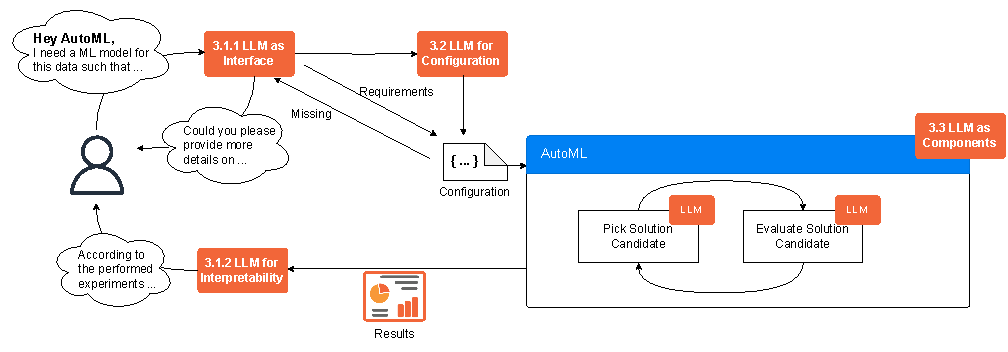
\includegraphics[width=1.\textwidth]{chapters/human-centric/llm/img/llms_for_automl_overview_3.pdf}
    \caption{Overview of options where \LLMs can be integrated into the \AutoML process.}
    \label{llm-fig:llms_for_automl_overview}
\end{figure}

\subsection{Opportunity I: Improving Human-Machine-Interaction with \LLMs}
\label{llm-ssec:hmi-with-llms}

As natural language has always been the cornerstone of human communication, advances in \NLP gave rise to an increasing amount of chatbots in various applications over the last decade \cite{adamopoulou-mla20}. Until recently, however, most of these chatbots have been rather limited in their capabilities. As ChatGPT \cite{openai-openai22a} shows, \LLMs have the potential to alleviate this situation by allowing for significantly more powerful chatbots and better textual interaction with a user. In the context of \AutoML, we foresee two promising directions: Leveraging \LLMs
\begin{itemize}
    \item as a user-friendly interface to \AutoML, and
    \item to improve the interpretability of the \AutoML process.
\end{itemize}


\subsubsection{Opportunity I.a:  \LLMs as an Interface to \AutoML}
\label{llm-ssec:llms-as-interface-to-automl}

The original promise of \AutoML was that it could automate some tasks of a data scientist to large degrees and thus democratize machine learning by allowing domain experts with little to no \ML knowledge to apply \ML to their domain. However, despite their success, many current \AutoML tools were not built around the user, but rather around algorithmic ideas. In particular, most of these tools allow for very limited interaction with a user in practice. This is also reflected in the reluctance of many researchers to use \AutoML tools \cite{blom-automl21a}. As a consequence, parts of the community have pushed towards a more human-centric \AutoML process aimed at supporting the data scientist such that they can work more efficiently \cite{lindauer-automlorg22,pfisterer-arxiv2019a}. Correspondingly, \AutoML can be seen to have two main target groups: 
\begin{itemize}
    \item Domain experts with little \ML knowledge who want to apply off-the-shelf \ML to their problem, and
    \item \ML experts who want to improve their workflow with automated tools that keep them in the loop. 
\end{itemize}
%
Right now, most \AutoML tools require coding or at least some technical understanding and, in terms of usability, target the second group much more than the first one. 

\LLMs enable us to fundamentally rethink how people interact with \AutoML systems and, in particular, help us design powerful interactive text-based interfaces such as chatbots. 
%By integrating audio capabilities, \AutoML systems powered by multimodal \LLMs can furthermore enable users to communicate with such systems through spoken language instead of text. 
%Such LLM-based interfaces then
These can iteratively extract the requirements of a user across a conversation and, in the background, configure an \AutoML system correspondingly (see also \Cref{llm-ssec:llms-for-configuring-automl}) based on \ML best practices and knowledge about optimization runs on similar datasets encoded in the \LLM. In particular, such interactive systems can simplify many of the complicated design decisions affecting the \AutoML process. For example, choosing an appropriate metric for optimization can be challenging for a non-expert, but might be possible with a competent interactive chatbot asking questions which guide the user to choosing the correct one. Naturally, this also bears the danger of wrong \AutoML configurations (see \Cref{llm-sec:dangers-and-challenges}).

Parts of this vision of conversational \AutoML assistants are already a reality with AI-based coding assistant tools such as GitHub Copilot \cite{copilot-github21a}. They can generate and suggest code to run \AutoML with the contextual information that the users give. Thereby, AI-based coding assistants already assist users in finding concrete \AutoML instantiations that best fit the requirement and the devices at hand. However, we envision assistants much more tailored to the needs of \ML practitioners. 

\subsubsection{Opportunity I.b: Interpretability of the \AutoML Process}
\label{llm-ssec:interpretability-of-results}

There has been a recent rise in methods trying to contribute to the aforementioned human-centric \AutoML paradigm \cite{pfisterer-arxiv2019a,lindauer-automlorg22,moosbauer-neurips21a,moosbauer-arxiv22a,segel-automl23a} by proposing ideas to improve the interactivity with the user and the interpretability of the \AutoML process. However, many of these works adapt rather classic interpretable machine learning methods to the \AutoML setting, whose results might remain rather complicated to understand for non-experts and do not provide any textual, easy-to-understand explanations. 

\LLMs have the potential to significantly increase the user-friendliness of those interpretations by elaborating on them in the form of text. In particular, an \LLM initialized with the history of evaluated configurations or pipelines, e.g. a run history from an optimizer such as SMAC \cite{lindauer-jmlr22a}, Hyperopt \cite{komer-automl14a} or BoTorch \cite{balandat-neurips20a}, as context could help generate a textual optimization report elaborating on the final \AutoML result and details of the process itself. Ideally, the \LLM could additionally be contextualized with results of several ixAutoML methods as a strong foundation for the report. This may even include images, such as partial dependence plots~\cite{moosbauer-neurips21a}, as multimodal \LLMs allow to process images as well~\cite{li-arxiv2023a, zhang-arxiv2023a}. If the user has questions about the report or elements not covered by the report, the \LLM could also be used as part of a chatbot to answer those questions. Although there is an ongoing discussion in the community on what constitutes a good explanation in general, textual explanations seem to be highly trusted by users \cite{gilpin-dsaa18a}.

\subsection{Opportunity II: \LLMs for Configuring \AutoML}
\label{llm-ssec:llms-for-configuring-automl}


\begin{figure}
    \centering
    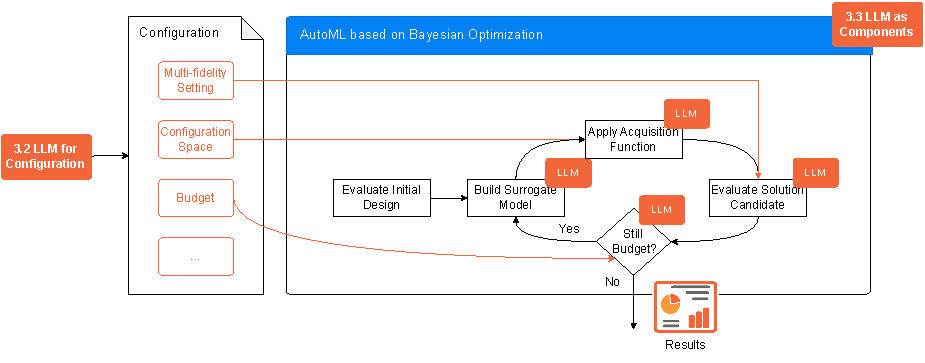
\includegraphics[width=1.\textwidth]{chapters/human-centric/llm/img/llms_for_automl_configuration.pdf}
    \caption{Visualization of the potential of \LLMs for the configuration of \AutoML (\Cref{llm-ssec:llms-for-configuring-automl}) and \LLMs as components of \AutoML systems (\Cref{llm-ssec:llms-for-simulating-automl}) at the example of a \AutoML process based on bayesian optimization.}
    \label{llm-fig:llms_for_automl_configuration}
\end{figure}

To fully shine, an \AutoML system must be set up correctly, including a suitable system configuration for the task at hand. Going even further, selecting among various \AutoML tools~\cite{thornton-kdd13a, feurer-nips15a, akiba-kdd19a, jin-sigkdd19a, erickson-arxiv20a, zimmer-tpami21a} can be important depending on the problem and hardware at hand. Although there exists work in the direction of removing the burden of selecting and configuring an \AutoML system \cite{feurer-automl18b,tornede-mlj22a,feurer-jmlr22a,moosbauer-tec22a}, setting up an \AutoML system without an expert can still be challenging. \LLMs offer a great opportunity to further improve this situation by suggesting a good configuration for the task at hand. Below and in Figure \ref{llm-fig:llms_for_automl_configuration}, we outline several configuration options, which are often very important but difficult to choose correctly, even for experts. 

The vast majority of \AutoML tools require the configuration of a search space of candidates from which solutions can be drawn. Depending on the concrete application, this usually spans several numerical, categorical, and ordinal hyperparameters -- often with dependencies between them. The concrete instantiation of this search space is crucial to find a well-performing pipeline quickly but is also hard to set up even for an expert. In particular, which kind of solutions (e.g. pipelines with or without preprocessing) are suitable, or which hyperparameters to tune and their concrete domains, are important to configure correctly. For example, choosing the domain of a hyperparameter to be small might benefit the search speed, but also bears the danger of missing the truly optimal value. Until now, this problem is either solved by an expert carefully configuring the \AutoML tool, by approaches that adaptively adjust the search space during the optimization process \cite{wistuba-ecml15a,nguyen-knowinfsys19a,hu-ieeetnnls22a,hu-eccv20a,chen-iccv19} or by integrating human expert knowledge as prior information guiding the search~\cite{souza-ecmlpkdd21a,hvarfner-iclr22a,mallik-metaws22a}.

Similarly important -- especially from a Green \AutoML perspective \cite{tornede-jair23a} -- is the question of how long to run the \AutoML process. Choosing a too-long runtime might waste both time and resources, while too-short runtimes bear the danger of missing good solutions. \LLMs could provide first settings for maximum runtimes of AutoML tools based on the experience from other AutoML practitioners. Going even one step further, we could even leverage the knowledge encoded in an \LLM to check whether the \AutoML run has already converged or whether further tuning could still be promising. Recent work by \citet{makarova-automlconf22a} has shown that such an automatic termination is in principle possible, even without \LLMs, and allows for considerable resource savings. In principle, we could even imagine that given a sufficient amount of \AutoML studies with details on the configuration space being tuned, an LLM could also learn how much \AutoML budget (e.g., in terms of evaluated configurations) is typically used for different configuration spaces to achieve a strong result.

Lastly, \LLMs could be used to configure the use of multi-fidelity approaches, such as Hyperband \cite{li-jmlr18a}. As recent work shows, the performance of multi-fidelity approaches is influenced by the choice of the fidelity types~\cite{deng-ecml22a} and the minimal/maximal amount of budget~\cite{bohdal-iclr2023a}. Correspondingly, choosing these correctly is crucial but also hard in practice, making an automated suggestion very helpful.

\subsection{Opportunity III: \LLMs as Components of \AutoML Systems}
\label{llm-ssec:llms-for-simulating-automl}

Most \AutoML systems are complex tools with a plethora of sub-systems and components that suit different purposes, such as estimating the performance of a pipeline \cite{white-neurips21a}, estimating the runtime of a pipeline \cite{mohr-tpami21a}, or choosing the next pipeline to evaluate. \LLMs offer the opportunity to replace many of these sub-systems as a meta-learned version thereof. Below and in Figure \ref{llm-fig:llms_for_automl_configuration} we outline and showcase several of such opportunities.

%acquisition function
Almost all \AutoML systems leverage some form of solution candidate selection strategy that selects the next candidate to be evaluated such as an acquisition function in BO-based systems. The knowledge modeling capabilities of \LLMs and their access to tremendous amounts of meta-data about ML and AutoML runs offer the opportunity to replace these mostly hand-designed selection strategies with a meta-learned version in the form of an \LLM. First works in these directions are promising: GPT-NAS \cite{yu2023gptnas} leverages a GPT model to predict (parts) of a neural architecture, i.e., a solution candidate based on an encoding which is used for evolving architectures. GENIUS \cite{zheng2023gpt4} even goes a step further and replaces the whole architecture suggestion step with GPT-4. It iteratively prompts GPT-4 for an architecture, which it evaluates, and re-prompts GPT-4 with the performance asking for a better architecture. This process is continued until a stopping criterion is reached. Similarly, EvoPrompting \cite{chen2023evoprompting} leverages an \LLM to implement the crossover and mutation operator in an evolutionary \NAS approach. Likewise, \citet{nasier-arxiv23a} suggest to leverage \LLMs to generate individuals in an evolutionary \NAS approach.

% feature engineering
Moreover, the knowledge encoded in \LLMs can also be used in feature engineering, as recently demonstrated. CAAFE \cite{hollmann2023gpt} is a feature engineering method for tabular datasets that leverages an \LLM to iteratively propose additional code for feature engineering based on their descriptions and feedback back the evaluation of this code piece to the \LLMs. This contributes beyond AutoML to the ultimate goal of automated data science \cite{bie-cacm22a}.

% solution evaluation and surrogate model
Furthermore, most \AutoML tools iteratively evaluate new solution candidates by training and validating. Naturally, this is a time-consuming process, especially if the training time of the solution candidate is extremely long, such as in deep learning. For this reason, some systems leverage meta-learned performance estimators such as meta-learned surrogate models in bayesian optimization~\cite{vanschoren-automlbook19a} or neural performance predictors in \NAS \cite{white-neurips21a} which can replace some of the evaluations. Once again, \LLMs offer a great opportunity to serve as a special form of meta-learned replacement based on knowledge extracted from large amount of unstructured data, which is not accessible to standard meta-learned approaches. They can also serve as a basis to generate training data for simpler performance/training time estimators or surrogate models and potentially also replace the latter. \citet{chen-neurips22a} have demonstrated that their OptFormer approach is able to learn both a competitive surrogate model and an acquisition function from the optimization history of Google's Vizier \cite{song-icml22b} platform.

% completely replace the \AutoML process
Going even further, both \citet{zhang-arxiv23b} and \citet{zhang-arxiv23a} suggest AutoML-GPT and MLCopilot, respectively, which fully work as a zero-shot \AutoML tool on their own. Given a textual problem description by the user and a knowledge base in the background, they suggest a pipeline and/or training procedure to achieve good performance on the specific problem. The problem itself can vary, but contains at least a description of the dataset a model is sought for, some form of search space description as a source of the model to be sought and a description on how performance is to be assessed. The search space can be a concrete class of models or even a concrete architecture such that the \LLM needs to find a complete pipeline or only good hyperparameters \cite{zhang-arxiv23b}. Note that these systems never evaluate a single \ML pipeline, but, in the case of AutoML-GPT, only use \LLMs to simulate the entire \AutoML process. \citet{tsai-arxiv23a} take a slightly different approach by using an \LLM to generate code to perform concrete \AutoML tasks in an iterative process which is controlled by another \LLM receiving the execution results and adjusting the prompt to the code \LLM correspondingly. Similarly, Aliro \cite{choi-bioinformatics23a} provide an \AutoML tool tailored towards medical data where \LLMs are used in the background to quickly generate code for user and case-specific analyses of the data.

The knowledge encoded in \LLMs can, in principle, be derived from a multitude of data sources, including but not limited to academic papers, data science and ML competitions (e.g., Kaggle), ML benchmark platforms (e.g., OpenML~\cite{casalicchio-19a}), \AutoML benchmarks, or \AutoML runs with their corresponding performances.
The increasing availability of open-source data and code may equip \LLMs with the capability to grasp intricate relationships between architectural choices, hyperparameters, performance outcomes, or runtimes.
Such data can be used to tailor \LLMs to specific tasks, as done for example in GPT-NAS \cite{yu2023gptnas}, which is pre-trained on the NAS-Bench-101 dataset \cite{ying-icml19a} and fine-tuned on a dataset adopting 36 presently prevalent neural architectures. However, the successes of \LLMs in performing \NAS \cite{zheng2023gpt4} or suggesting a whole \AutoML pipeline \cite{zhang-arxiv23a, zhang-arxiv23b}, even without fine-tuning, suggests that the models can generalize their understanding from the wealth of information available.

All of the examples above crucially depend on how the prompts for the \LLM are designed and how the knowledge gained so far is added as context to the prompts. For example, EvoPrompting \cite{chen2023evoprompting} adds the code of all previously evaluated architectures together with their evaluation results as an annotation to the prompt as context. Naturally, this can quickly lead to very large prompts, which can be challenging for current \LLMs, although recent work tries to alleviate the prompt size limitation \cite{yu-arxiv23a}.

\section{Risks}
\label{llm-sec:dangers-and-challenges}
%(1-2 pages)

Besides the numerous valuable ways to integrate \LLMs and \AutoML, the combination poses some risks. Below, we elaborate five risks combining \LLMs and \AutoML:

\begin{enumerate}
    \item Using \LLMs for configuring \AutoML requires extracting meta-knowledge about \AutoML tasks to be fed into the \LLMs. Therefore, intensive and human-time-consuming prompt engineering is required to reliably extract that knowledge.
    \item The usage of publicly available data to evaluate \AutoML approaches configured via \LLMs might be data snooping, as the \LLM might have already seen the data during training. The detection of prior knowledge of an \LLM about a given dataset becomes more and more important.
    \item \LLMs are known to hallucinate from time to time, presenting false facts due to the lack of fact-checking. This could be crucial when \LLMs are used to configure \AutoML as inappropriate configurations could be used.
    \item The full-text interaction of \LLMs seems to be quite trustworthy for laypeople, although the presented content might not be true at all. In combination with \AutoML, the user might mistakenly get a positive impression of the results.
    \item Combining two resource-intensive research areas, i.e. \LLMs and \AutoML, will result in an even more resource-intensive research area. Thus, it is more important to be transparent about the resources used and find ways to be more efficient.
\end{enumerate}

\subsection{Risk I: Complicated Human-Interaction} We have leveraged the working assumption that \LLMs trained on a large corpus of text also encode knowledge about \AutoML tasks several times throughout this manuscript. Such knowledge could comprise a general understanding of what models perform well given a dataset description or which preprocessing is required for a specific task at hand. However, extracting such knowledge for the user in a reliable way depends on the specific prompt, leading to the task of prompt engineering for \AutoML \cite{sorensen-etal-2022-information}. Ideally, human-machine-interaction will make designing a concrete prompt obsolete by automatically constructing it in an automated fashion from a chat-like interaction with a user. However, this might only work to a certain extent and currently remains an open problem. Correspondingly, we risk that by leveraging \LLMs for \AutoML we only shift the barrier of entry from requiring coding and \ML knowledge to prompt engineering knowledge.

\subsection{Risk II: Evaluation}
Any form of evaluation of an \AutoML approach leveraging \LLMs in some component needs to be performed with care. As \LLMs are trained on extreme amounts of unstructured data, it is quite likely that they see many openly available \ML datasets during training including corresponding test data or a condensed version thereof, such as a model trained on the data. Thus, evaluating an \AutoML pipeline that uses an \LLM on a dataset that was part of the training data of the underlying \LLM is akin to data snooping \cite{kok-us1984}. Correspondingly, the evaluation result would be strongly biased. We see two main strategies to circumvent this problem: First, we could evaluate it on datasets that are guaranteed not to have been seen by the \LLM during training, such as data generated after the \LLM has been trained \cite{faggioli2023perspectives}. Naturally, this raises the question of how to get such private datasets, which are still freely accessible for other researchers, of realistic nature in order to compare approaches, but still were not used by the \LLM in advance. Second, we could try to fine-tune an \LLM to remove any knowledge about a dataset from its model~\cite{yang-arxiv22a}. To achieve this, we would need to know how to detect prior knowledge of the \LLMs about any used dataset or a condensed version thereof. Once such knowledge is detectable, we would need to find a way to reliably remove it via fine-tuning. However, at this point in time, there is no approach guaranteeing that prior knowledge about a dataset can be fully removed. Overall, the evaluation of an \AutoML system featuring an \LLM is far from trivial and requires new protocols.  

\subsection{Risk III: False Facts and Misuse}
\LLMs are known to generate output sounding confident but featuring hallucinated knowledge \cite{ji-acmcs23a}, which might be indistinguishable or at least hard to distinguish from facts in some cases. Correspondingly, we may wonder whether any usage of \LLMs within \AutoML systems can lead to detrimental results, e.g., when misconfiguring the \AutoML via an \LLM by the user such that almost no runtime is granted, or the \LLM takes decisions like choosing the search space which might be inappropriate for the given problem. 
A potential solution to this might be the integration with a knowledge graph \cite{hogan-acmcs22a} tailored towards \AutoML that can be used as a knowledge base to contextualize potential \LLM suggestions. Moreover, we should consider filters or safeguards for degenerate solutions output by the \LLM and resolve to predefined defaults in those cases.

In general, when integrating \LLMs with \AutoML systems, we should keep in mind the potential for wrong \LLM output and how such output can be detected in a probabilistic approach. A big advantage over many other disciplines is that we can validate whether replies by the \LLM are correct by simply running an experiment and comparing the experiment result output by the \LLM and the result we obtain from the run \cite{zheng2023gpt4,chen2023evoprompting,hollmann2023gpt}.

\subsection{Risk IV: Trust and Explanations}
Although improving the human-machine-interaction of \AutoML systems leveraging \LLMs (Sec.~\ref{llm-ssec:hmi-with-llms}) has the potential to democratize \ML even more, it also bears dangers when more laypeople interact with such systems. For example, due to the full-text interaction with a user, there might be a lot of trust in the results, although the returned machine learning model might not be suitable for the given problem at all. Correspondingly, the attention of the user should be drawn to potential ambiguities in the interaction, and they should be made well aware of the assumptions the overall system makes due to the textual interaction. One way to address this issue could be to add further explanation approaches telling users how certain replies were generated~\cite{deb-arxiv23a}. 

\subsection{Risk V: Resource Consumption} 
Both \LLMs and \AutoML are resource-intensive research areas on their own. Combining them could lead to even higher resource consumption, raising the question if spending these resources is worth it. In view of the growing number of fine-tuned \LLMs for medical applications~\cite{han-arxiv23a,wu-arxiv23b}, it is quite likely that there will also be fine-tuned \LLMs for specialized \AutoML tasks. With the potential of easily generating more and more meta-knowledge for \AutoML by simply evaluating more \ML pipelines or hyperparameter configurations, it could even lead to a race of repeatedly fine-tuned tasks.\footnote{We note that in contrast to real \NLP tasks where human input is required, it is much easier to generate new examples of how \ML pipelines or \AutoML systems behave and perform.} Nevertheless, the potentially rich meta-knowledge stored in these \LLMs (see \Cref{llm-ssec:llms-for-configuring-automl}) could also lead to new efficiency gains in \AutoML. Overall, in the spirit of Green \AutoML \cite{tornede-jair23a}, it will be even more important to be transparent about the resources used when conducting research at this intersection, and to find ways to be more efficient on both sides.

\section{Conclusions}
\label{llm-sec:conclusion}

\LLMs already started to have big impact on \AutoML, both how \AutoML is designed for \LLMs, and how \LLMs can be leveraged for \AutoML. 
Nevertheless, we are only at the beginning of a long journey to solve the many challenges and make use of the opportunities while considering the risks ahead of us. We strongly believe that we, as a community, will overcome those challenges and savour the remarkable opportunities that an integration of \LLMs and \AutoML offers.

The biggest challenge of all can be boiled down to one fact: The training and maintenance of the most capable \LLMs requires immense resources, such that only a few groups worldwide are able to provide those systems. This implies several problems for the community: \begin{itemize}
    \item We are not easily able to study how \AutoML can be tailored toward training of \LLM base models;
    \item We cannot easily check which data was used to train the models which bears risks in using and evaluating \LLMs for \AutoML;
    \item We cannot easily add safeguards against misuse of \LLMs and \AutoML.
\end{itemize}
Correspondingly, it is even more problematic that the responsibility and control over \LLMs lie in those few hands of mostly private companies. In view of this, we believe that one of the next steps has to be the development an open-source \LLM with the specific goals of the \AutoML in mind.



\part{Physics-aware AI}\label{part:physics-aware}
% \chapter{Formalization}
\label{precision-chap:formalization}

\chapter{An Auto-Tuning Three-Dimensional Numerical Model Coupled with Data Assimilation from a Sensor Grid}
\label{physics-aware-chap:orchard}

\chapter{Multi-Sensor Profiling for Precision Soil-Moisture Monitoring}
\label{physics-aware-chap:pluto}

Controlling soil moisture is a crucial factor in optimizing watering and crop performance \cite{turkeltaub2016real}.
For instance, in our case study, kiwifruit (\emph{Actinidia deliciosa}) -- in short kiwi -- has high water demand \cite{judd1986water}, cultivated in countries such as New Zealand, Chile, and Italy.

Different types of watering systems may be adopted depending on the farming features and needs; typical solutions exploit drippers, sprinklers, hose reels, and flooding.
In orchards, where a stable watering system can be built, drip irrigation is widely used as it enables precise watering that, in turn, reduces water waste.

\paragraph{Challenges}
The risks of over-watering range from groundwater depletion to plant suffocation.
As to kiwi, farmers tend to over-water since it leads to larger fruits, but this reduces their dry mass and jeopardizes their maintenance after harvest.
Ideally, the moisture level should be known and optimal on the whole soil volume taken by the tree roots.
Such volume is subject to strong horizontal and vertical variability caused by many related factors, among them: (i) uneven root suction, (ii) limited watering-system coverage, and (iii) difference in the soil layers in terms of composition and exposure to atmospheric agents. %, (iv) punctual anomalies of the ground (e.g., hysteresis).

\Cref{pluto-fig:soilvolume} shows an example of an orchard watered through a single-pipeline dripper system.
Each cube shows the soil volume taken by the roots.
On the one hand, the limited distance between drippers ensures homogeneous moisture (i.e., the watered volume in blue) \textit{along the row} (i.e., multiple trees in the same line).
On the other hand, the effect of watering drops \textit{across the rows} (i.e., between two lines of trees), and a portion of the soil volume remains completely unwatered (i.e., the volume in orange).

When the watered volume is symmetric along the row, as in \Cref{pluto-fig:soilvolume}, a 2D grid (\Cref{pluto-fig:sensorgrid}-left) is sufficient to represent the entire soil volume. Conversely, when relevant moisture variations take place along the row too, a 3D grid (\Cref{pluto-fig:sensorgrid}-right) is more suitable. Such variations may be determined, for example, by too sparse drippers or by non-homogeneous suction of the roots.

\begin{figure}[t]
\centering
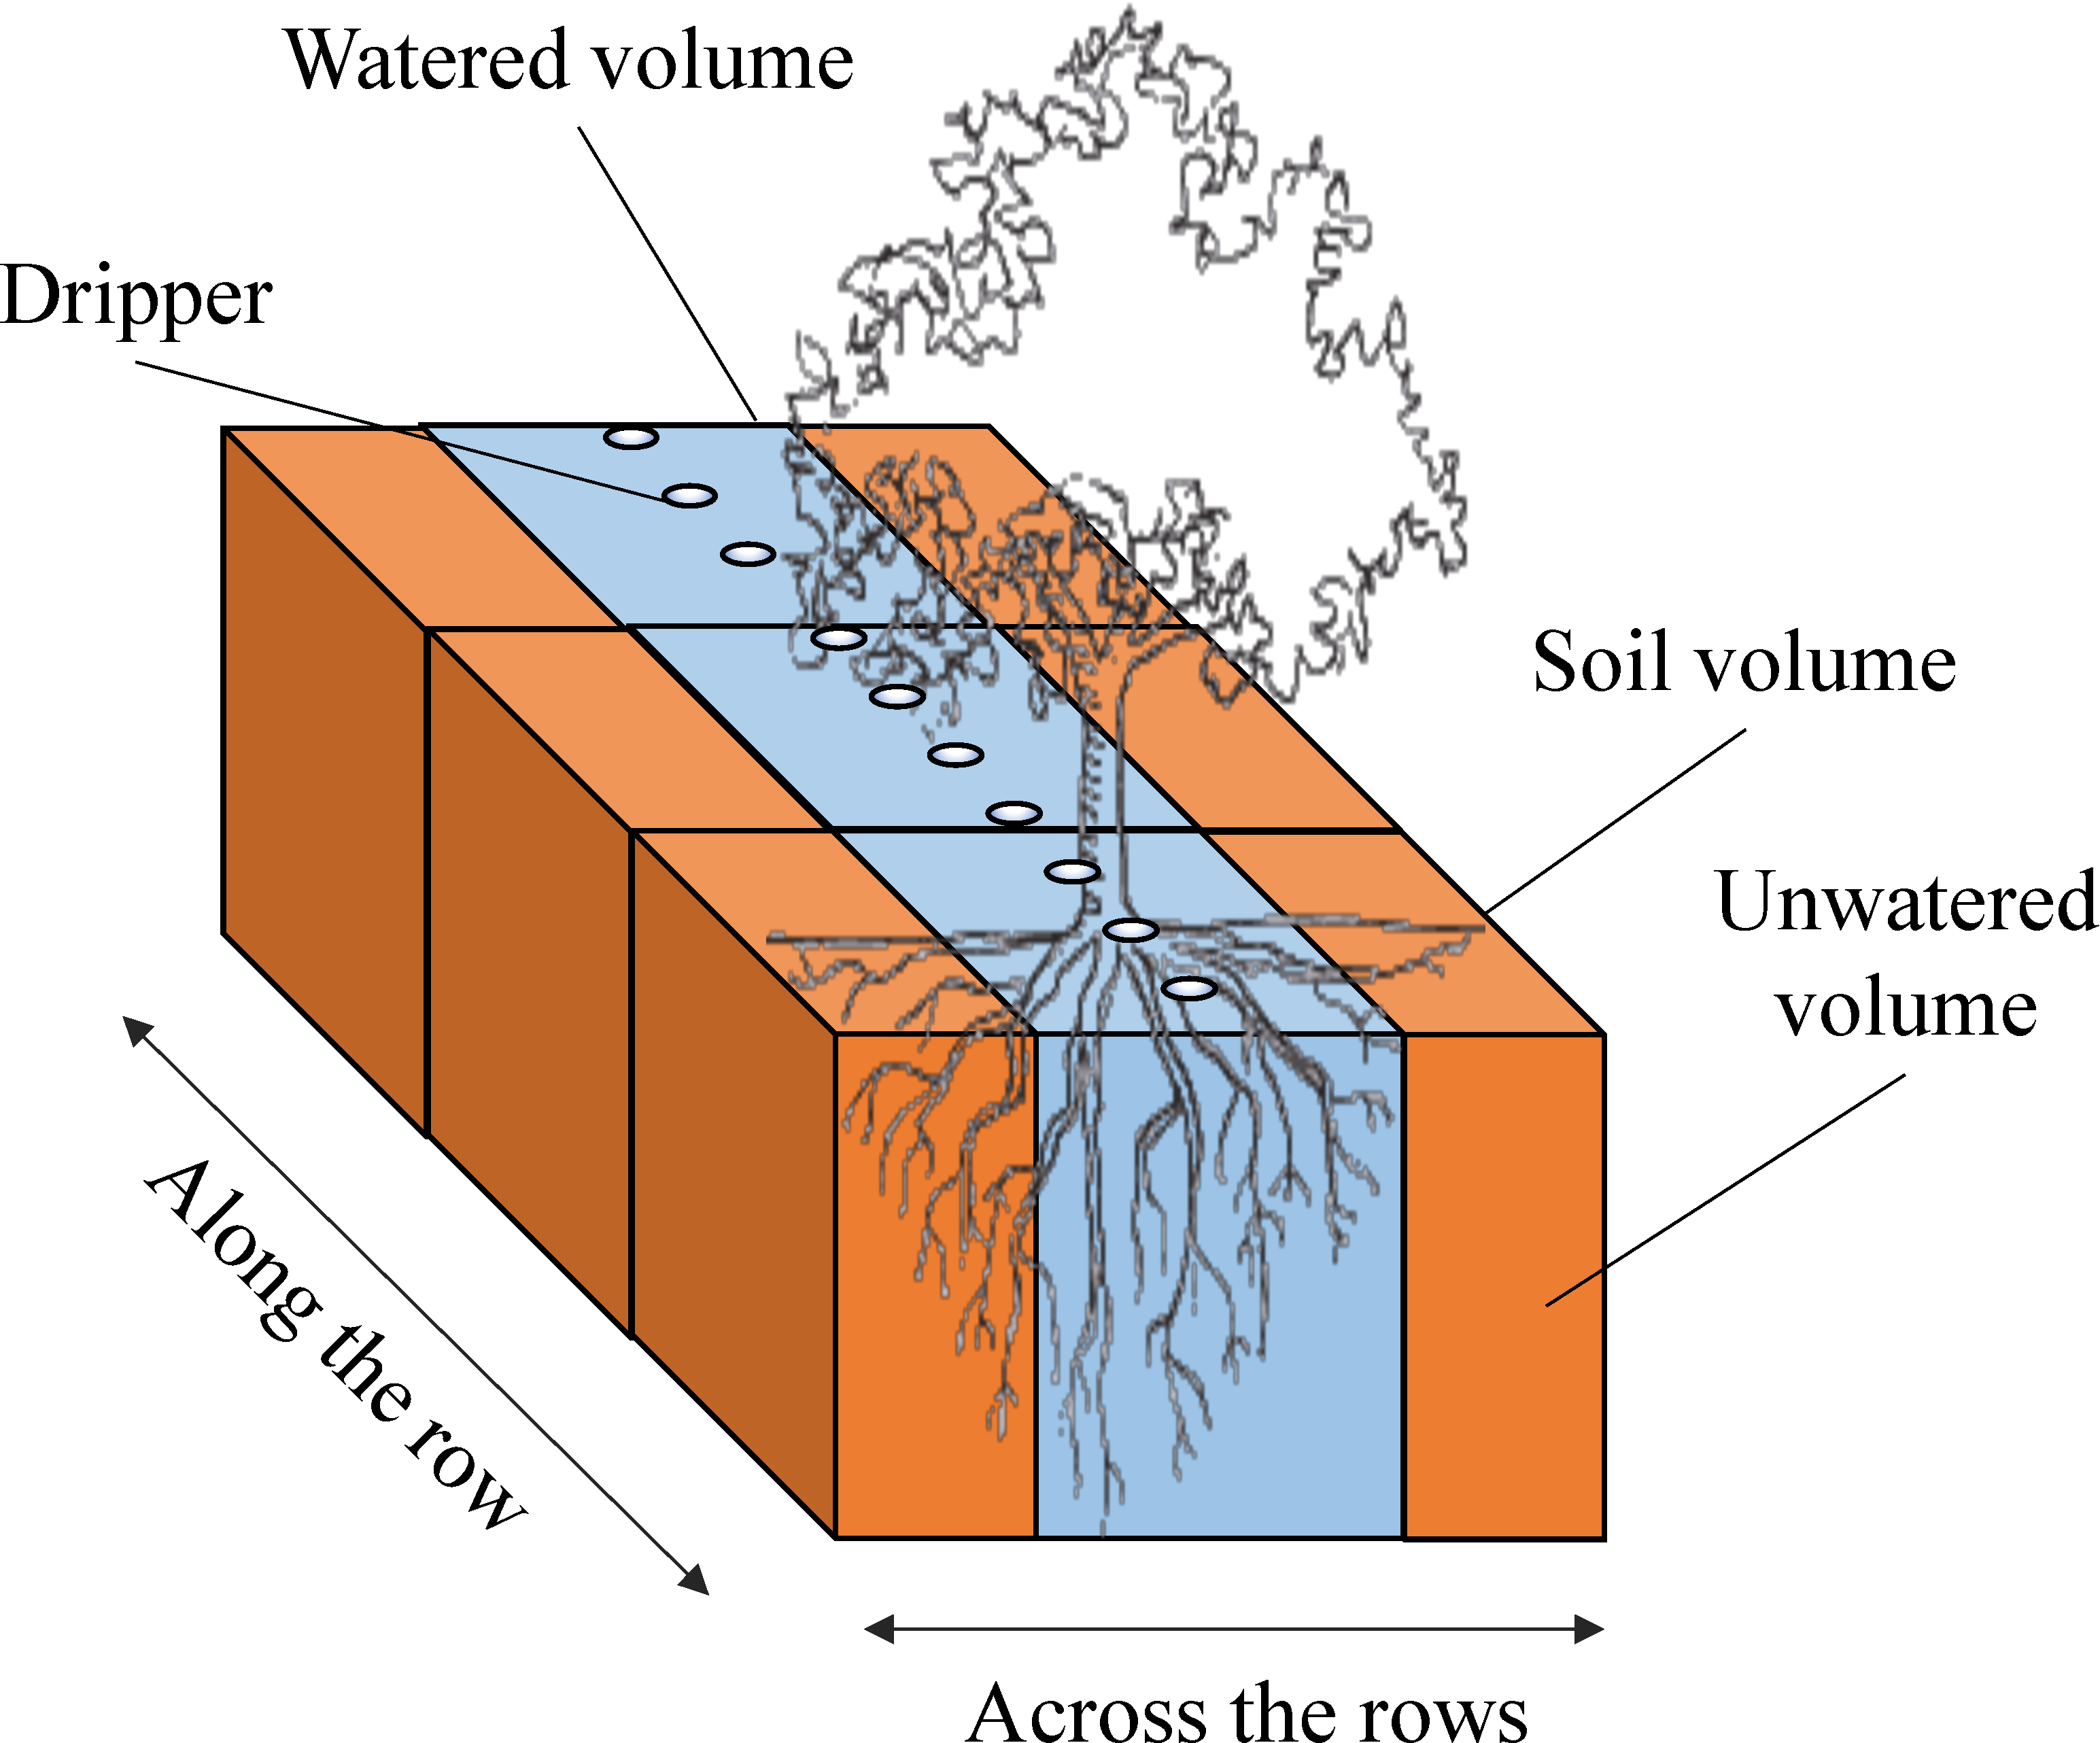
\includegraphics[scale=.14]{chapters/physics-aware/pluto/img/SoilVolume2.pdf}
\caption{Relevant elements in a orchard.}
\label{pluto-fig:soilvolume}
\end{figure}

\begin{figure}[t]
\centering
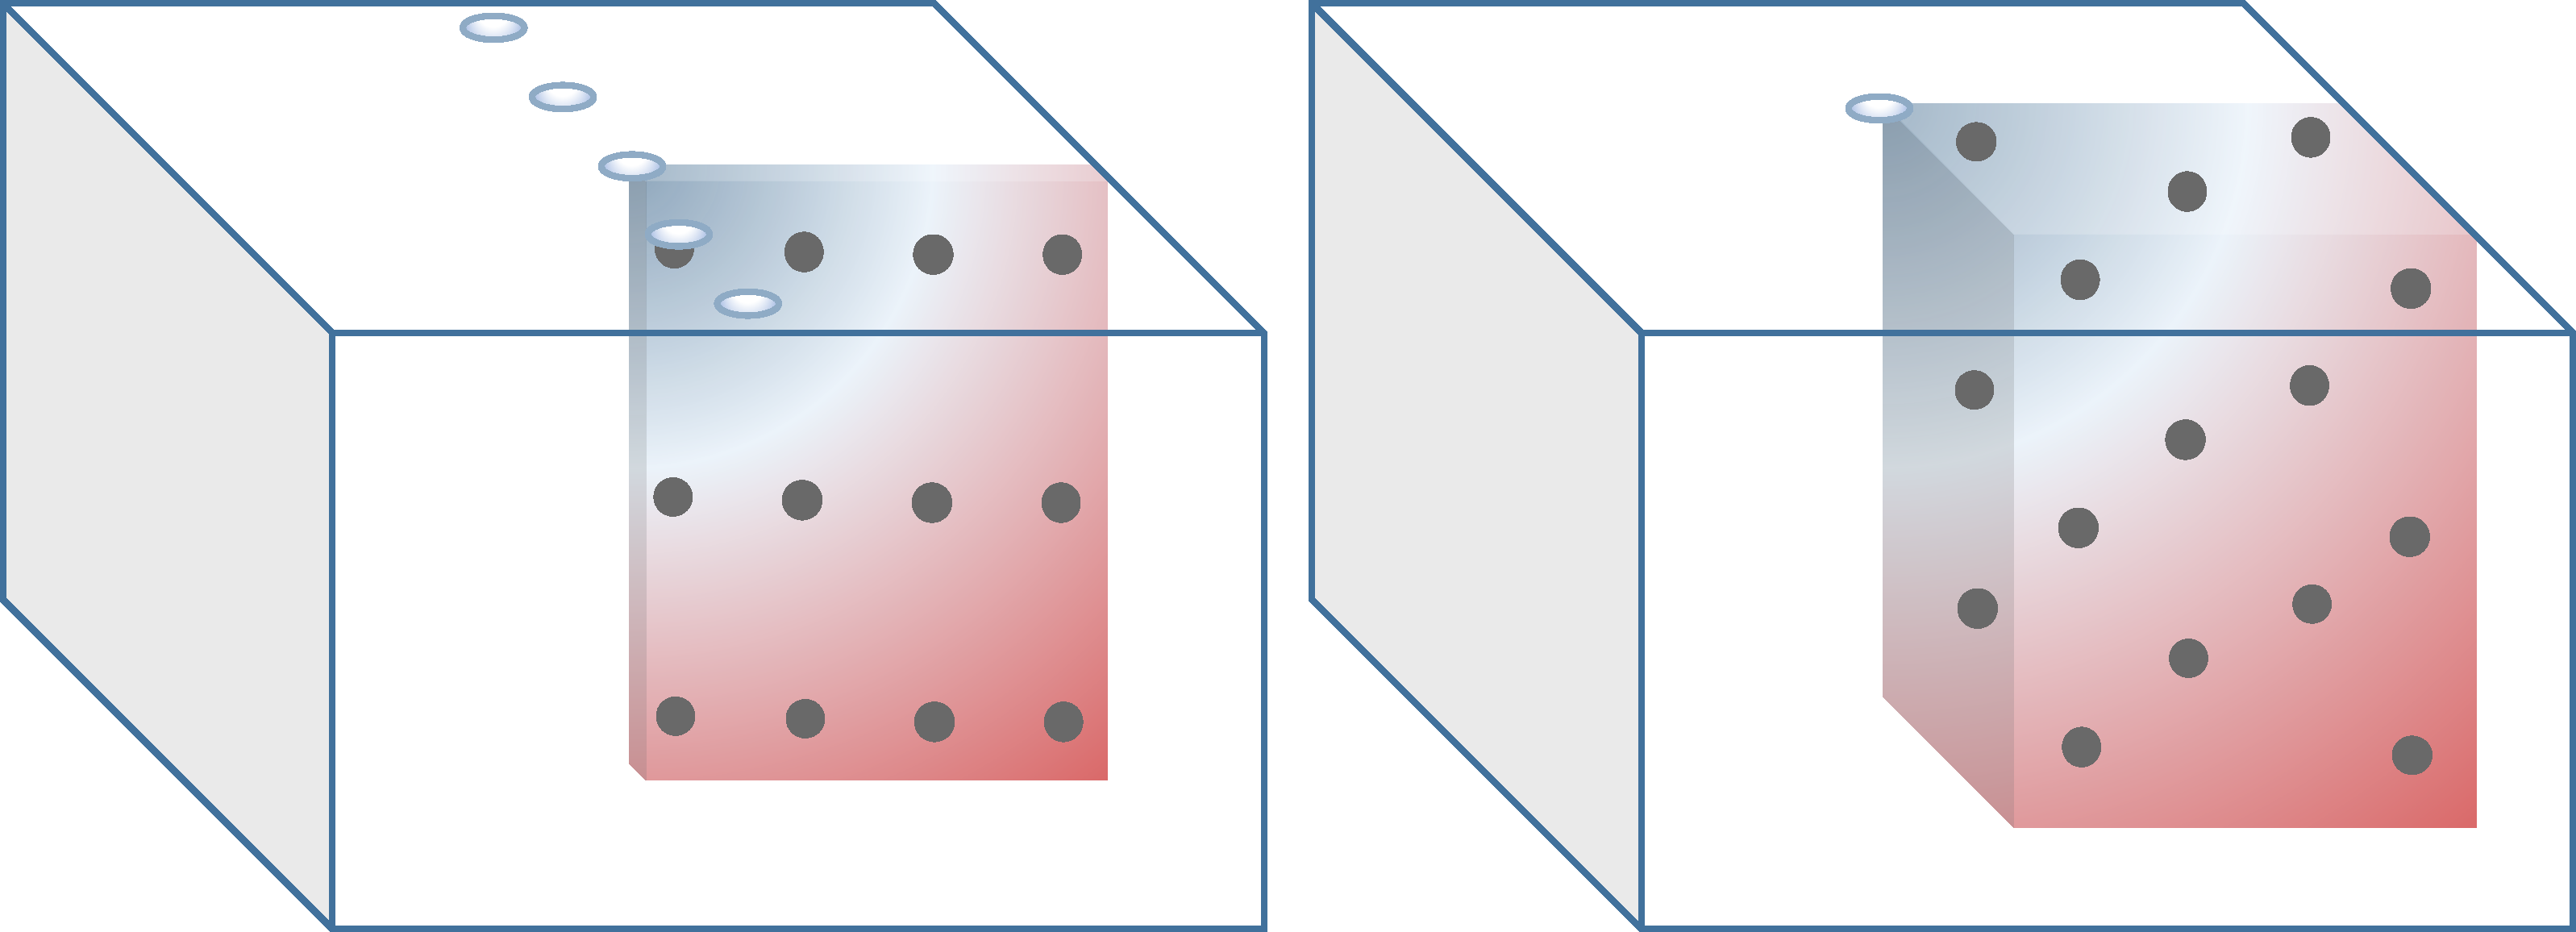
\includegraphics[scale=.21]{chapters/physics-aware/pluto/img/SensorGrid2.pdf}
\caption{Regular 2D (left) and 3D (right) sensor grids.}
\label{pluto-fig:sensorgrid}
\end{figure}

\paragraph{Contributions} The main application of our work is preserving an optimal moisture level without wasting water.
Our approach, named PLUTO\footnote{In Greek mythology, god of wealth. His name is linked to the prosperity of crops.}, focuses on the following contributions.
\begin{itemize}
    \item The concept of 2D/3D moisture profile (i.e., a fine-grained representation of moisture in a portion of soil) based on a grid of sensors. 
    The grain of the profile is in the order of magnitude of square/cubic centimeters.
    \item Two alternative solutions to estimate a fine-grained profile by adopting linear and non-linear approximations.
    In particular, non-linear approximation relies on an artificial neural network that learns a model of soil moisture given the soil texture.
    \item An analysis of the trade-off between the accuracy, the number, and the position of sensors.
    \item Several original profile visualizations that enable visual exploitation of the profile.
\end{itemize}

To the best of our knowledge, PLUTO is the only approach aimed at creating a fine-grained multidimensional profile of soil moisture given a sensor grid.
Our goal is to provide a cost-effective and operative solution that monitors soil moisture and whose reference application is \textit{long-term} watering optimization.
Previous approaches building a soil profile -- such as \cite{Hinnell2010535} -- do not utilize any real soil moisture measurements, relying solely on simulations with process-based models.
Yet, to correctly model all the soil phenomena (e.g., water tables, hysteresis), it is well-known that realistic simulations require tuning with real sensor data.

% For instance, \cite{Hinnell2010535} exploit HYDRUS as a process-based model to provide fine-grained samples and Artificial Neural Networks as a ML model to extract subsurface wetting patterns.
% With respect to PLUTO, \cite{Hinnell2010535} (i) produce a statistical representation of the patterns that is based on a \textit{single} dripper and assume a \textit{uniform} characterization of the soil, (ii) derive the wetting patterns from generic soil parameters and not from actual sensor values.
% However, they do not utilized any real soil moisture measurements to calibrate the numerical model.
% Indeed, it is well-known that realistic simulations with process-based models require real soil moisture measurements to correctly model all the soil phenomena (e.g., water tables, hysteresis).
% In particular, previous approaches building a soil profile -- such as \cite{Hinnell2010535} -- exploit sensors to calibrate a simulator (e.g., HYDRUS \cite{hydrus2008587}) and thus (i) require long time series of data from the field; (ii) bind the profile exploitation to an expensive and resource-consuming simulation; and (iii) require frequent updates.
% For these reasons, such approaches typically carry out \textit{spot} researches to study soil moisture dynamics.
% Conversely, our goal is to provide a cost-effective, operative solution that monitors soil moisture and whose reference application is \textit{long-term} watering optimization.

The remainder of this chapter is organized as follows.
% \Cref{pluto-sec:background} introduces the basics of soil moisture monitoring and surveys the previous related works in such an area.
\Cref{pluto-sec:MaterialsAndMethods} describes PLUTO in detail, \Cref{pluto-sec:ResultsAndDiscussion} reports the tests carried out on real data collected over two years, and \Cref{pluto-sec:conclusions} draws the conclusions.

% We emphasize that our work is one of the outcomes of the Agro.Big.Data.Science project \cite{ABDS}.
% The project, funded by Regione Emilia Romagna, aims to study and implement digital solutions to support smart and precision farming.

\section{PLUTO}
\label{pluto-sec:MaterialsAndMethods}
\begin{figure}[t]
\centering
\begin{subfigure}[t]{.3\textwidth}
\centering
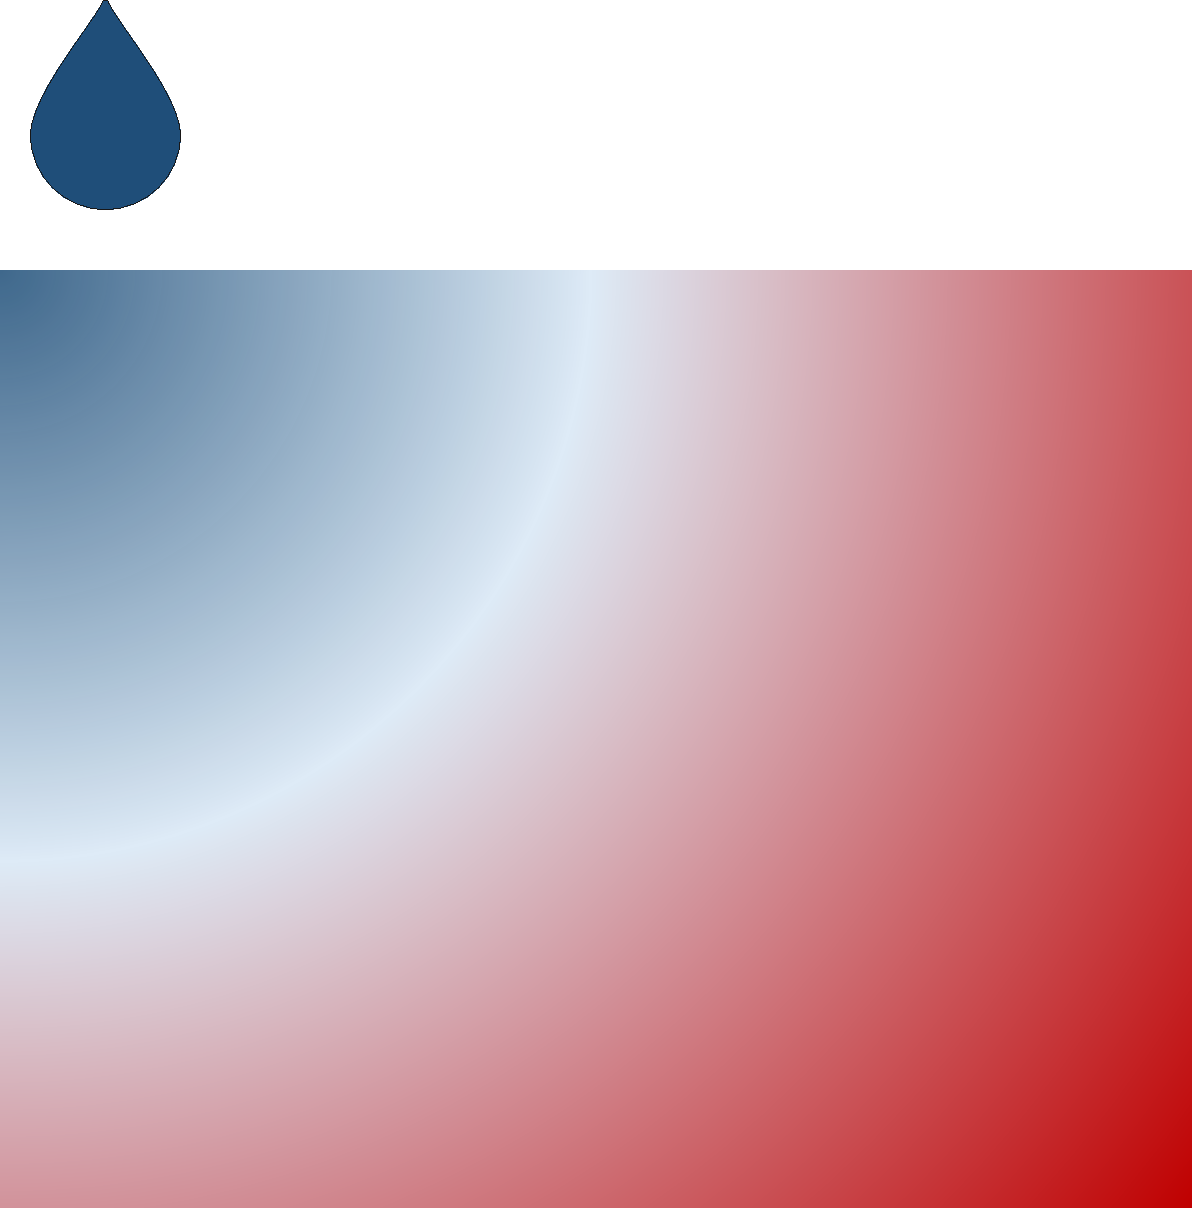
\includegraphics[scale=.15]{chapters/physics-aware/pluto/img/soil-moisture-continuous.pdf}
\caption{Actual soil moisture.}
\label{pluto-fig:moisture-cont}
\end{subfigure}~
\begin{subfigure}[t]{.3\textwidth}
\centering
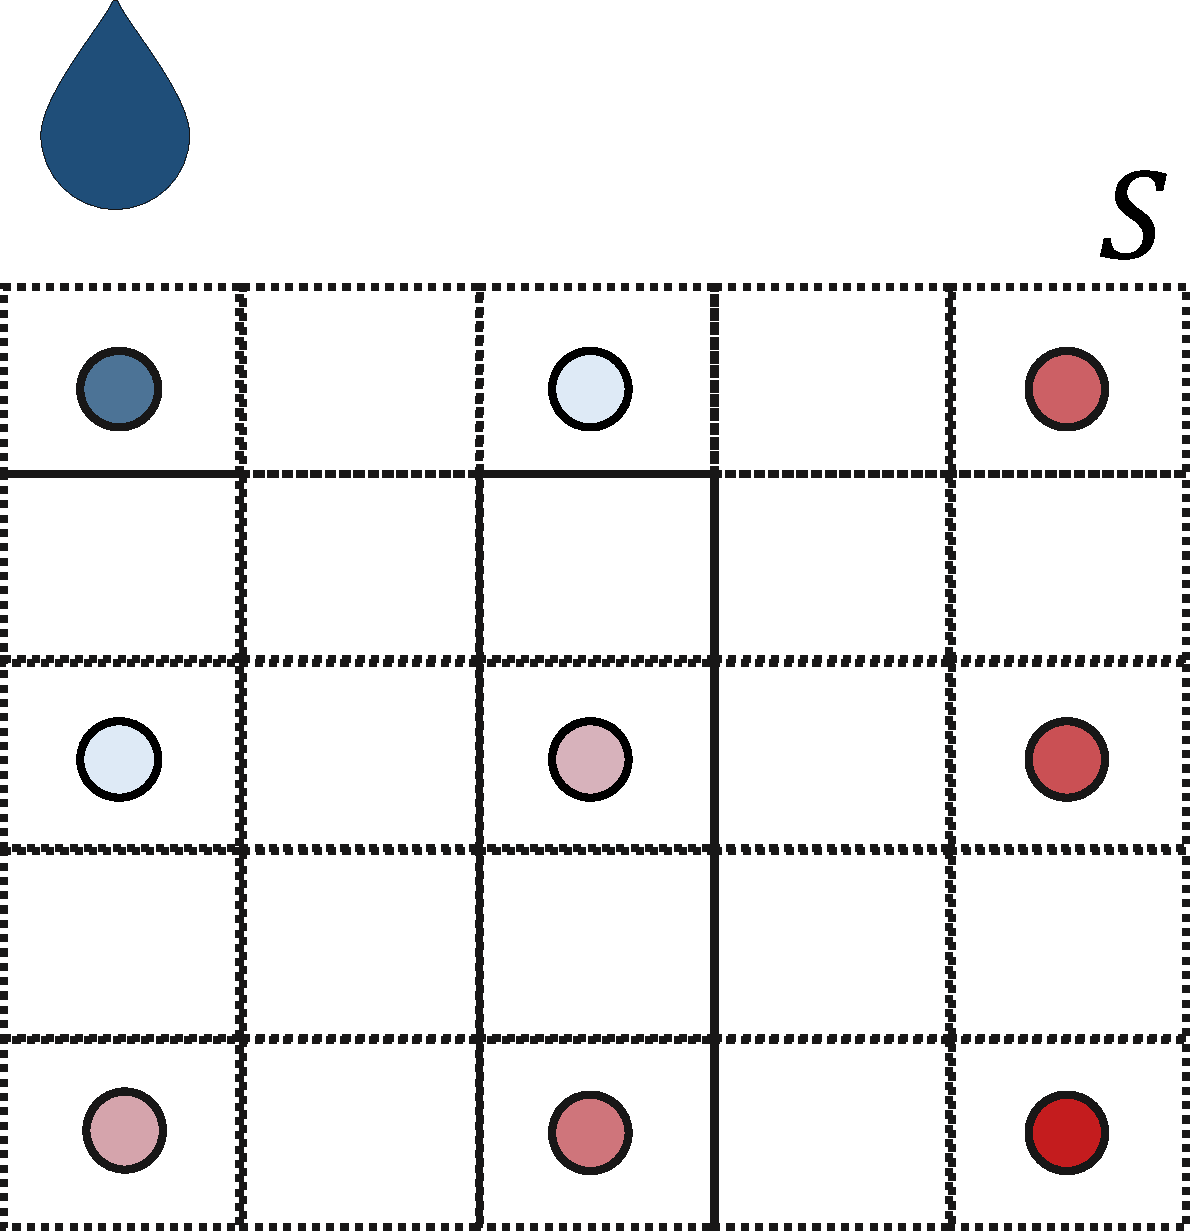
\includegraphics[scale=.15]{chapters/physics-aware/pluto/img/soil-moisture-sample.pdf}
\caption{Raw sensor grid}
\label{pluto-fig:moisture-sens}
\end{subfigure}
~
\begin{subfigure}[t]{.3\textwidth}
\centering
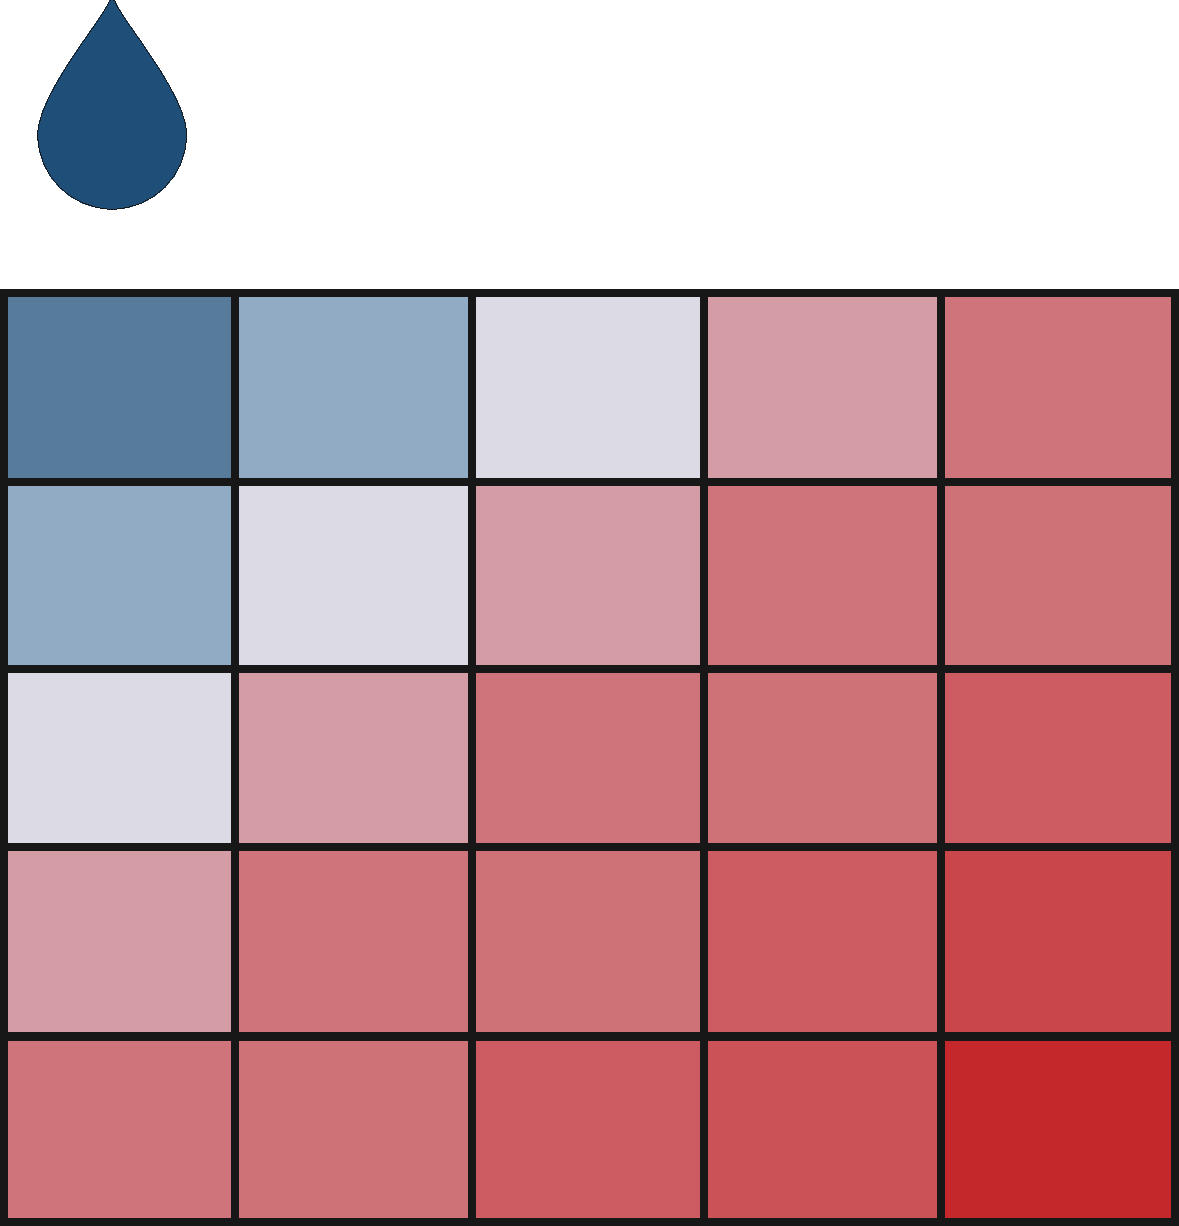
\includegraphics[scale=.15]{chapters/physics-aware/pluto/img/soil-moisture-profile.pdf}
\caption{Soil profile}
\label{pluto-fig:moisture-profile}
\end{subfigure}
\caption{Snapshot of soil moisture in a soil slice; the water drop represents a dripper.}
\label{pluto-fig:moisture}
\end{figure}

Our goal is to create a moisture profile that represents the whole soil volume.
\begin{definition}[Soil Volume]
Given a tree, its \emph{soil volume} is a parallelepiped of soil that contains most of the tree roots. The soil volume is centered in the tree position.
\end{definition}

\begin{definition}[Sensor Grid]
A \emph{sensor grid} $S = \{s^1, ..., s^{|S|}\}$ is an $n$-dimensional layout of $|S|$ sensors installed in a soil volume.
Each \emph{sensor} $s^i$ is defined by a three-dimensional displacement $(s^i.x_1, s^i.x_2,s^i.x_3)$ with respect to the center of the soil volume, and by a soil moisture value $s^i.v$.
\end{definition}


Depending on $n$, the grid resembles a line ($n=1$), a rectangle ($n=2$) or a parallelepiped ($n=3$). The monitored value depends on the sensor technology; typically sensors measure volumetric water content or the soil potential. \Cref{pluto-fig:installation} shows one of the Agro.Big.Data.Science project installations \cite{ABDS} located in Faenza (Emilia Romagna, Italy).
This orchard is watered through a single pipeline of drippers (distance between drippers 40cm) and soil moisture is monitored through a 2D sensor grid of 12 gypsum block sensors.

\begin{figure}[t]
    \centering
    \begin{subfigure}[t]{.5\textwidth}
    \centering
    \includegraphics[scale=.145]{chapters/physics-aware/pluto/img/sensors-satellite.png}
    \end{subfigure}~
    \begin{subfigure}[t]{.5\textwidth}
    \centering
    \includegraphics[scale=.4]{chapters/physics-aware/pluto/img/sensors.jpg}
    \end{subfigure}
    \caption{A sensor grid is monitoring soil moisture close to a kiwi tree near Faenza, Italy. The watering system is composed of single-pipeline drippers.}
    \label{pluto-fig:installation}
\end{figure}

Soil moisture varies continuously within the soil volume while the raw sensors provide point-wise measurements.
Furthermore, in most real-world applications, the number of sensors is by far less than those we used in our research project; this further reduces the comprehensiveness of the measurements.
For instance, companies involved in Agro.Big.Data.Science \cite{ABDS} relied on 1 to 3 sensors disposed at different depths (i.e., a 0D or a 1D grid).
The moisture profile, based on raw sensor measurements, estimates soil moisture of the whole soil volume at a fine-grained resolution.

\begin{definition}[Moisture Profile]
Given an $n$-dimensional sensor grid $S$, the \emph{moisture profile} is an $n$-dimensional grid $P = \{p^1, ..., p^{|P|}\}$ that approximates, in each $p^i$, the soil moisture measured by $S$. $P$ is \emph{fine-grained} with respect to $S$ since $|P| > |S|$. 
\end{definition}

The approximation $p^i.v$ is assumed to be constant in the region surrounding $p^i$, whose granularity depends on $|P|$.

\begin{example}
Given a 2D sensor grid covering an area of $0.6 m^2$ (i.e., a rectangle with a width of $1m$ and a height of $0.6m$), we employed a sensor grid with 12 sensors (i.e., $|S| = 12$) and a moisture profile with 1000 points (i.e., $|P| = 1000$). As a result, we obtained a moisture profile having a granularity of $6 cm^2$ (i.e., $0.6 m^2 / 1000$) while the sensor grid granularity is $500cm^2$ (i.e., $0.6 m^2 / 12$). For the sake of clarity, \Cref{pluto-fig:moisture-sens} shows a sensor grid with $|S|=9$ and \Cref{pluto-fig:moisture-profile} shows a moisture profile with $|P|=25$.
\end{example}

A moisture profile covers the sensor grid region that is typically smaller, in size and dimensionality, than the soil volume. To provide a comprehensive estimation of the whole soil volume, we rely on the following assumption of \emph{symmetry}: the portions of the soil volume that are not covered by the sensor grid behave as the monitored one; in other words, the profile of the uncovered portions can be obtained under rotation or translation of the moisture profile.
\Cref{pluto-fig:symm} shows the symmetries in the case of 2D and 3D grids.
The symmetry assumption is verified for 2D grids when the drippers along a tree row are close enough to ensure homogeneous soil moisture.
If the distance between the drippers is high and the soil moisture along the row is not constant, a 3D grid must be adopted to satisfy the symmetry assumption.
Obviously, a 3D grid does not require any symmetry assumption if sensors are distributed all around the tree.
However, given a fixed amount of sensors, not exploiting the assumption of symmetry results in a coarser grid.

We emphasize that all the soil moisture estimation approaches based on sensors implicitly make symmetry assumptions: if a single sensor (0D installation \cite{arif2013estimation}) is used, the measured moisture is assumed as the reference value for the whole soil volume (i.e., it is assumed to be constant all over the soil volume); if a column of sensors (1D installation \cite{Karandish2016892, Goldstein2018421, Jimenez20201327, Pan2021, Li20152382}) is used the moisture is considered constant at a given depth. From this point of view, PLUTO's 2D and 3D grids progressively lighten such assumptions leading to a more accurate result. Obviously, some assumptions of symmetry remain, but they seem reasonable especially in the agricultural context: orchard rows are (or can be) built to be symmetrical. For example, the kiwi orchards involved in the Agro.Big.Data.Science project (i) were north-south oriented to have the same sun exposure on both the sides of the row; (ii) exploit a T-Bar training system; (iii) have a symmetric raised bed (i.e., with the same slope on both sides of the row).
More in general, to handle the variability within a single installation, it is always possible to design a grid layout that involves both sides of the row and, to handle variation within different parts of the field, two replicas can be installed.
In the following, \Cref{pluto-sec:FromSensorsToMoistureProfile} details the implementation of how switch from sensors to moisture profiles (i.e., via profiling functions), \Cref{pluto-sec:visualization} illustrates the visual components of PLUTO.

\begin{figure}[t]
\centering
\includegraphics[scale=.6]{chapters/physics-aware/pluto/img/SensorGrid3.pdf}
\caption{Symmetries in watered soil: dotted rectangles (left) or parallelepipeds (right) replicate the data collected by the sensor grids.}
\label{pluto-fig:symm}
\end{figure}

\subsection{From Sensors to Moisture Profile}
\label{pluto-sec:FromSensorsToMoistureProfile}
The transformation of raw sensor measurements into a moisture profile is achieved through a profiling function.
\begin{figure}[t]
\centering
\includegraphics[width=1\textwidth]{chapters/physics-aware/pluto/img/process.pdf}
\caption{Feature-aware and feature-unaware processes for building a moisture profile.}
\label{pluto-fig:process}
\end{figure}
\begin{definition}[Profiling Function]
Given an $n$-dimensional sensor grid $S$ and a moisture profile $P$, a \emph{profiling function} $f : S \rightarrow P$ approximates the values of the moisture profile $P$ starting from the sensor grid $S$.
\end{definition}

The role of a profiling function is approximating the soil moisture values in those positions of the moisture profile where a sensor is not present. 
A profiling function is based on sensor grid measurements and can optionally exploit further information about the behavior of the soil. 
Several profiling functions can be adopted. 
We propose two alternative approaches that differ in the information exploited.
\begin{itemize}
    \item \emph{Soil-feature-unaware} - FU: exploits the sensor measurements only. The most obvious choice is to carry out a linear interpolation between pairs of sensor values.
    \item \emph{Soil-feature-aware} - FA: exploits the knowledge about soil hydrological dynamics to keep into account non-linearities and to get a more accurate estimation.
\end{itemize}

\Cref{pluto-fig:process} sketches the two alternative profiling functions and
% The feature-unaware function does not require to be fitted to a specific field and only gets sensor data as input, while the feature-aware function is trained offline to capture non-linear behaviors that result in a more accurate moisture profile.
\Cref{pluto-fig:FU_FA} exemplifies their main differences showing the profiles obtained by applying such functions to a grid of four sensors on the corners.
The values for the sensors are the same for the two profiles (top-left=-10cbar, top-right=-300cbar, bottom-left=-200cbar, bottom-right=-300cbar).
The profile on the left is obtained by applying the feature-unaware profile function, while the one on the right by applying the feature-aware function.
We note that the former has issues in capturing non-linearities in soil moisture dynamics; yet, we also emphasize that this is a worst-case scenario as our feature-unaware function also captures non-linear behaviors.
Indeed, using a grid of sensors, we are implicitly adopting a local regression approach \cite{loader2006local,cleveland1988locally}.
Although local regression approaches are bound to linear behavior between sensor pairs, the composition of several linear strokes can approximate a non-linear trend.
Conversely, our feature-aware function models the non-linearities between sensor pairs too.
The lower level of soil moisture in the upper right part results from the combination of two factors that are better captured via information wrt. the soil: this region (i) is proximal to the surface (thus it is more subject to atmospheric events) and (ii) belongs to the unwatered volume.
The gap between the two approximations grows as the distance between the sensors increases.

\subsubsection{Feature Unaware Profiling Function}

We rely on the well-known $n$-linear interpolation, where $n$ is the profile grid dimensionality.
For the sake of conciseness, in the following, we describe the $2$-linear case. 
Given a 2D sensor regular grid $S$, this technique carries out a linear interpolation in each dimension independently from each other.
The approach consists of two phases (\Cref{pluto-fig:statistical-profiling-function-explanation}).
For each point $p \in P$ of the moisture profile to be computed: (i) we find the four sensors $S$ that determine the minimum bounding rectangle enclosing $p$ (\Cref{pluto-fig:statistical-profiling-function}), then (ii) we compute $p.v$ (\Cref{pluto-fig:bilinear-interpolation}) by interpolating along the $x_1$ axis first. Then, exploiting the obtained points $r$  (blue dots), interpolation is performed along the $x_2$ axis and the value $p.v$ is finally determined.
Below follows the formal definition.

\begin{figure}[t]
\centering
\begin{subfigure}[t]{.45\textwidth}
\centering
\includegraphics[scale=.4]{chapters/physics-aware/pluto/img/statistical_profiling_function.png}
\caption{Bounding rectangle for $p$}
\label{pluto-fig:statistical-profiling-function}
\end{subfigure}
~
\begin{subfigure}[t]{.45\textwidth}
\centering
\includegraphics[scale=.4]{chapters/physics-aware/pluto/img/bilinear_interpolation.png}
\caption{Bilinear interpolation}
\label{pluto-fig:bilinear-interpolation}
\end{subfigure}
\caption{A 2D example of the feature-unaware function.}
\label{pluto-fig:statistical-profiling-function-explanation}
\end{figure}


\begin{align*}
    r^{ij}.v &= \frac{s^j.x_1-r^{ij}.x_1}{s^j.x_1-s^i.x_1} s^i.v + \frac{r^{ij}.x_1-s^i.x_1}{s^j.x_1-s^i.x_1} s^j.v\\
    r^{hk}.v &= \frac{s^k.x_1-r^{hk}.x_1}{s^k.x_1-s^h.x_1} s^h.v + \frac{r^{hk}.x_1-s^h.x_1}{s^k.x_1-s^h.x_1} s^k.v \\
    p.v &= \frac{r^{ij}.x_2-p.x_2}{r^{ij}.x_2-r^{hk}.x_2} r^{hk}.v + \frac{p.x_2-r^{hk}.x_2}{r^{ij}.x_2-r^{hk}.x_2} r^{ij}.v
\end{align*}
The trilinear procedure is analogous: it just has three steps instead of two.


\subsubsection{Feature Aware Profiling Function}
The feature-aware function captures non-linear soil moisture behaviors by exploiting the knowledge about the hydrological fluxes. To this end, we rely on an artificial neural network (ANN) \cite{bishop1994neural}, a ML model, that returns the estimated values for each profile point after learning the soil behavior from the data generated by CRITERIA \cite{Bittelli2011253}, a process-based model.
%\jgc{}{The ANN profiling function,} Given the sensor measurements, \jg{we leverage an Artificial Neural Network (ANN)} that returns the estimated values for each profile point.
The learning process is sketched in \Cref{pluto-fig:process}.
The ANN learns the soil behavior from simulated data in an off-line phase, which is carried out only once at the time of installation of the system.
%We rely on a \jg{crop simulation model??} \cite{Bittelli2011253}  to create the training dataset.
CRITERIA reproduces hydrological fluxes in the soil volume implementing Richard's equations.
The simulator models the following elements of the soil volume: (i) the soil texture; (ii) the shape of the tree roots; (iii) the watering system type and layout; and (iv) the sensor layout.
Such data are provided as input by the farmer.
Then, training data are generated running the simulator according to simulated weather conditions and watering sessions.
Generating hourly data over a 4-month period proved to be sufficient to train the ANN.

ANNs have been chosen for the feature aware profiling function due to the following properties:
\begin{itemize}
    \item Low resource consumer: once trained offline, the ANNs are fast and require limited computational resources. 
    \item Powerful \& Flexible: can provide accurate profiles (i.e., they properly capture non-linearities) even though the grid layout includes a limited number of sensors. 
    \item Robust: ANNs are well-known to work well even in case of dirty or missing data. This may happen when a sensor occasionally fails to provide the correct data. 
\end{itemize}

\begin{table}[t]
\centering
\caption{The ANN hyperparameter configuration retrieved by HyperOpt.}
% \scriptsize{
\begin{tabular}{lc}
\hline
Hyper-parameter & Value \\ \hline
\# Hidden Layers & 1 \\
\# Neurons per layer & 100 \\
Activation function & Tanh \\
Normalization & Z-score \\
\# Training epochs & 50 \\
Batch size & 30 \\
Reduce learning rate & factor=2, patient=10 \\ \hline
\end{tabular}
% }
\label{tab:ann_configuration}
\end{table}

\Cref{tab:ann_configuration} reports the hyperparameters for the PLUTO ANN.
We adopted a feed forward ANN (i.e., neurons in the layers are connected without creating any cycle) with one, fully connected, hidden layer.
The input layer has one neuron for each sensor, the hidden layer has a hundred of neurons activated through the hyperbolic tangent activation function (e.g., values of the neurons are mapped according to the homonym mathematical function), and the output layer has as many neurons as the number of points in $P$ (see \Cref{pluto-fig:ANN}).
As to the learning hyperparameters, the process involves 50 epochs, a batch size of 30 samples, and the learning rate (i.e., the step size towards the final solution) is reduced by a factor of 2 when no improvement is seen for a \textit{patient} number of 10 epochs.
%The neurons are activated through the hyperbolic tangent activation function.
Besides, a Z-score normalization (i.e., transforming data into a Gaussian distribution with mean 0 and standard deviation 1) is applied to the input values before feeding the network. This is due to the following reasons.
\begin{figure}[t]
\centering
\includegraphics[scale=.4]{chapters/physics-aware/pluto/img/ANN.pdf}
\caption{The layout of the ANN profiling function.}
\label{pluto-fig:ANN}
\end{figure}

\begin{itemize}
    \item To give all the input values the same importance. Even though the soil moisture varies everywhere in the same range, we noticed sensible variations depending on the location of the sensor (e.g., the area right under the dripper and the opposite corner).
    \item To address ANN-specific training issues. Normalizing the inputs reduces the chances of getting stuck in local optima (e.g., balance the rate at which the ANN learns) and makes training faster (e.g., avoid the saturation of non-linear activation function).
\end{itemize}

All the hyperparameters (i.e., ANN structure and learning rates) have been set through a hyperparameter tuning process implemented with HyperOpt \citep{bergstra2015hyperopt}. HyperOpt exploits state-of-the-art optimization techniques to heuristically explore the huge search space of hyperparameters. The adoption of a training set including several different weather conditions and watering sessions avoids overfitting (i.e., a learning process that returns a network that works well just for the specific cases it was trained for).


\begin{figure}[t]
\centering
\includegraphics[scale=.25]{chapters/physics-aware/pluto/img/countor_plot.pdf}
\caption{Moisture profile built by the two types of profiling functions, namely feature-unaware (left) and feature-aware (right).}
\label{pluto-fig:FU_FA}
\end{figure}

\subsection{Visualization}
\label{pluto-sec:visualization}
Visualization allows easy exploitation of the moisture profile, enabling effective soil moisture monitoring.
We propose two visual components selected according to the data types and the following visualization goals \cite{golfarelli2020model}.
\begin{itemize}
    \item \emph{Historical soil moisture trend}: shows the variation of moisture over time.
    Independently of the profile dimensionality, a 2D stacked area chart is adopted.
    No spatial information is shown here.
    \item \emph{Spatial soil moisture}: shows the spatial distribution of soil moisture at a specific time. A 2D heat map or a 3D scatter plot is adopted depending on the profile dimensionality.
\end{itemize}
The two components are linked through \emph{interactive zooming} \cite{keim2002information}. When the user selects a specific time on the historical soil moisture trend, the corresponding spatial soil moisture at the time is shown.

Since the goal is to check that an ideal moisture profile is maintained, we define five crop-specific soil moisture ranges, each associated with a different color.
For our case of study on kiwi-trees \cite{ABDS}, Dark blue (in $[0, -30)$ cbar) and light blue (in $[-30, -100)$ cbar) show heavily/slightly portions of over-watered soil. Salmon pink (in $[-100, -300)$ cbar) represents the ideal case \cite{miller1998effects}.
Finally, light red (in $[-300, -1500)$ cbar) and dark red (in the range of $[-1500, -\infty)$ cbar) show slightly/heavily portions of under-watered soil.

\begin{figure}[t]
\centering
\includegraphics[scale=.12]{chapters/physics-aware/pluto/img/2d-visualization.pdf}
% \caption{A 2D-visualization example.}
\caption{Visualization of a 2D profile: (left) the historical soil moisture and (right) a snapshot of the spatial soil moisture. The rightmost legend shows the soil moisture ranges. The drop at depth $0$ represents the \textit{Dripper} position and the rightmost legend shows the soil moisture ranges.}
\label{pluto-fig:2D-visualization}
\end{figure}

\Cref{pluto-fig:2D-visualization} shows examples of historical soil moisture trend and spatial soil moisture charts for a 2D profile.
The historical soil moisture chart shows how the soil gradually dries out during the dry season.
In May the soil is mostly wet, while in June the first irrigations are necessary. 
Also, note how the single pipeline dripper fails to eliminate the red area due to the presence of an unwatered region in the soil volume.
For the chosen zoom date, the spatial soil moisture chart shows the moisture profile in detail. Each cell corresponds to a profile element.
The following areas can be highlighted: (i) the region under the dripper where the effects of irrigation are apparent; (ii) the superficial portion away from the dripper that is very dry as it is not irrigated; and (iii) the deep region which is less affected by atmospheric agents and in which constant soil moisture remains regardless of the effects of watering.
The profile highlights how the soil moisture spreads laterally thanks to the combined effect of the roots and the permeability characteristics of the soil.

\begin{figure}[t]
\centering
\begin{subfigure}[t]{.45\textwidth}
\centering
\includegraphics[scale=.4]{chapters/physics-aware/pluto/img/3d-visualization-a.png}
\end{subfigure}
~
\begin{subfigure}[t]{.45\textwidth}
\centering
\includegraphics[scale=.45]{chapters/physics-aware/pluto/img/3d-visualization-b.png}
\end{subfigure}
% \caption{A 3D visualization during a rotation.}
\caption{Visualizing rotations of a 3D profile.}
\label{pluto-fig:3D-visualization}
\end{figure}

\Cref{pluto-fig:3D-visualization} shows an example of a 3D spatial soil moisture chart.
Each sphere corresponds to a profile element. The colors are the same as in the 2D visualization.
Spaces between spheres allow the inner side of the 3D profile to be explored. Furthermore, to facilitate the analysis, the chart can be rotated along the three axes. 
The soil moisture gradient along the third dimension (i.e., along the row) is better highlighted by the third orientation of the chart and justifies the adoption of a 3D profile.

Starting from the spatial profile, we derive many meaningful visualizations. \Cref{pluto-fig:variazione-umidita-profilo}-left shows the profile variance chart, which reports the soil moisture variance in a given period.
The lighter areas are those where soil moisture varies the most. Similarly, \Cref{pluto-fig:variazione-umidita-profilo}-right shows the profile average chart which reports the average soil moisture in a given period.
The charts are designed to support the work of both agricultural technicians and farmers. For example, in the Agro.Big.Data.Science projects the main questions posed by such users were:
\begin{itemize}
    \item \emph{What is the watered volume?}:
    this region is typically characterized by two phenomena: high moisture and high suction by the roots.
    Depending on the supplied quantity of water, the summation of the two phenomena determines different effects.
    In the case of over-watering, the watered volume remains always wet, with high values in the average chart and low values in the variance chart as the roots and the atmospheric phenomena are not able to absorb the water.
    Conversely, in the case of correct irrigation, the average chart shows medium values while the variance one shows high values mainly due to the suction made by the roots. This is the case for \Cref{pluto-fig:variazione-umidita-profilo}. 
    \item \emph{Where is the root suction higher?}: 
    a high root suction quickly reduces the moisture in the soil and results in a strong soil moisture variance. 
    \item \emph{How soil moisture dynamics impact on the watered volume?}: if, after increasing the quantity of water supplied to the soil, the watered volume does not increase significantly, then the soil disperses water in depth due to its characteristics.
\end{itemize}
In the context of the Agro.Big.Data.Science project agricultural technicians and some \emph{data enthusiast farmers} \cite{morton2014support} already had the competences to directly exploit the charts, while most of the farmers had been trained. We strongly believe that the progressive digitization in agriculture will drive all farmers to take advantage of these solutions, as it has already happened to operators in other industries.

A demo of the PLUTO visualization system is available at \url{https://big.csr.unibo.it/projects/pluto}. The monitoring system can be completed by the following information collected through a weather station and a water meter:
\begin{itemize}
    \item a single line chart showing the max/min/avg air temperature;
    \item a bar chart showing the mm of rain that fell each day;
    \item a bar chart showing the mm of water supplied, each day, through watering. 
\end{itemize}
Although the role of data processing and visualization is often overlooked, such visualizations contribute to a comprehensive understanding of the evolution of the profile.

\begin{figure}[t]
\centering
\includegraphics[scale=.25]{chapters/physics-aware/pluto/img/countor_plot_std_mean.pdf}
\caption{Soil moisture variance (left) and average (right) in cbar along a 1-week period; the orchard is watered through a single-pipeline dripper system.}
\label{pluto-fig:variazione-umidita-profilo}
\end{figure}

\section{Empirical Evaluation}
\label{pluto-sec:ResultsAndDiscussion}
We tested PLUTO on the installations of the Agro.Big.Data.Science project \cite{ABDS}.
Data have been collected in the irrigation season from May to September in 2020 and 2021.
Installations are taken from two orchards: one in the plains and one in the hills around Faenza, in the province of Ravenna, Italy.
The orchards were planted in 2010 as a self-rooting Hayward variety (A. chinensis var deliciosa), grafted in 2012 with Gold 3 (A. chinensis var chinensis). 
kiwifruit vines were spaced 2m along the row and 4.5m across the rows.
Different irrigation systems and sensor grid layouts have been considered as shown in \Cref{pluto-tbl:implants}.
Sensor data are sampled and collected every 15 minutes. 
% Please add the following required packages to your document preamble:
% \usepackage{booktabs}
\begin{table}[t]
\centering
% \footnotesize{
\begin{tabular}{@{}ccccccc@{}}
\toprule
Location & \# Grids & Grid Layout & \# sensors & Watering system \\ \midrule
Hilly & 1 & 3D & 15 & Single pipeline \\
Hilly & 2 & 2D & 12 & Single pipeline \\
Hilly & 2 & 2D & 12 & Double pipeline \\
Plain & 4 & 2D & 12 & Single pipeline \\ \bottomrule
\end{tabular}
% }
\caption{Description of the experimental implants.}\label{pluto-tbl:implants}
\end{table}

We emphasize that the number of sensors we use is much higher than necessary, as we will show below. 
Grids with 12-15 sensors were used to build the ground truth to carry out the tests. In each test only a subset of the available sensors was used to compute the profile, while the remaining ones were used as ground truth. In other words, we verify how well the profile approximates the soil moisture in positions where the real soil moisture is known to the tester but hidden to PLUTO. Profile accuracy is calculated as the Root Means Square Error (RMSE) between the ground truth sensor values and the values estimated by the profile. Obviously, the RMSE is computed only for those sensors that are not used to compute the profile.

\subsection{Accuracy Evaluation}
\label{pluto-sec:ApproachEvaluation}
\Cref{pluto-fig:2Dperformance} shows the system performance, for the 2D profile, varying the number of input sensors. Tests have been repeated for all the available installations.
To better understand the advantage provided by PLUTO, we also highlighted the performance of profiling based on a single sensor --- 0D setting --- (i.e., the \emph{de facto} standard) or a column of 3 sensors at different depths --- 1D setting. 
To extend the soil moisture value of the single sensor to the entire soil volume, we must assume the soil moisture to be constant in the whole volume. 
Similarly, when a column of sensors is available, we assume that soil moisture is constant at the same depth in the soil.
Since the accuracy varies based on the sensor location, we choose the single sensor position (or the sensor line) that minimizes the RMSE as a fair comparison baseline.
The same methodology was adopted to displace the sensors used to calculate the profile. 
We refer to section \Cref{pluto-sec:sensors_disposal_evaluation} for an in-depth analysis of the layout of the profile sensors and the robustness of the system.

The 0D setting estimations are by far less accurate than the ones obtained by our profiling functions; indeed, three sensors are sufficient to halve its RMSE using the feature-aware profiling function. 
The 1D setting achieves slightly better results since it captures soil moisture at different soil depths, but fails in capturing longitudinal variations. 
The extent of these errors is not negligible since the optimal range for soil moisture for kiwi cultivation is $[-100;-300)$ cbar \cite{miller1998effects}.

RMSE for feature-aware and feature-unaware gradually decreases as the number of sensors increases. 
Note that the bilinear profiling function can be computed only for some sensor layouts, due to the intrinsic geometrical constraints (i.e., the profile region must be partitioned in bounding rectangles/cubes). 
The ANN profiling function always outperforms the bilinear one due to its capability to better model non-linear behaviors. 
This supremacy is more evident when the number of sensors is limited and the intra-sensor distances are larger (see \Cref{pluto-fig:FU_FA}). 
\begin{figure}[t]
\centering\
\includegraphics[scale=.5]{chapters/physics-aware/pluto/img/bar_plot.pdf}
\caption{2D profile performances as a function of the input  sensors. Single sensor (0D) and column (1D) settings are reported for comparison. }
\label{pluto-fig:2Dperformance}
\end{figure}

\begin{figure}[t]
\centering\
\includegraphics[scale=.5]{chapters/physics-aware/pluto/img/3d_bar_plot.pdf}
\caption{3D profile performances as a function of the input  sensors. Single sensor (0D), column (1D) settings, and (2D) profile are reported for comparison.}
\label{pluto-fig:3Dperformance}
\end{figure}

3D profile performances are reported in \Cref{pluto-fig:3Dperformance}. This type of profile measures soil moisture variability along the row, while 2D profiles assume soil moisture to be constant along the row. 
The chart shows that the assumption is partially true since the RMSE for the 2D profile (i.e., the dotted line) is higher than those related to the 3D ones. 
The RMSE further increases for the 0D and 1D settings as they progressively make stronger assumptions about symmetry. 
As expected, the RMSE for the 3D profiles decreases as the number of sensors increases, and the feature-aware profiling function overcomes the feature-unaware one.

%\begin{figure}[t]
%\centering
%\begin{subfigure}[t]{.4\textwidth}
%\centering
%\includegraphics[scale=.45]{chapters/physics-aware/pluto/img/single-pipe-2.pdf}
%\end{subfigure}
%~
%\begin{subfigure}[t]{.4\textwidth}
%\centering
%\includegraphics[scale=.45]{chapters/physics-aware/pluto/img/double-pipe.pdf}
%\end{subfigure}
%\caption{Profile comparison for orchards equipped with single pipeline dripper (left) and double pipeline dripper (right) watering systems. The cell labeled with letter \emph{D} at depth $0$ shows the \textit{Dripper} position.}
%\label{pluto-fig:pipeline-comparison}
%\end{figure}
\begin{figure}[t]
\centering\
\includegraphics[scale=.13]{chapters/physics-aware/pluto/img/single-double-pipeline.pdf}
\caption{Profile comparison for orchards equipped with single pipeline dripper (left) and double pipeline dripper (right) watering systems. The drop at depth $0$ represents the \textit{Dripper} position and the rightmost legend shows the soil moisture ranges.}
\label{pluto-fig:pipeline-comparison}
\end{figure}

Overall, 2D and 3D profiles are much more accurate; they better capture variations in soil moisture than the baselines (that are traditionally used in commercial settings). \Cref{pluto-fig:pipeline-comparison} highlights the ability to identify different soil behaviors by showing the dynamics of soil moisture in fields with different watering systems. The orchard reported in \Cref{pluto-fig:pipeline-comparison}-left adopts a single-pipeline dripper system where the pipeline is placed along the row. 
The orchard in \Cref{pluto-fig:pipeline-comparison}-right adopts a double-pipeline dripper system were each pipeline is shifted by 20cm on the right/left of the tree row.
As shown by the profile, the compound effect of the raised bed and the shift of the pipeline determines a heavily different soil moisture diffusion.
This effect can only be pointed out using 2D or 3D profiles.

\subsection{Sensor Layout Analysis}
\label{pluto-sec:sensors_disposal_evaluation}
As shown in \Cref{pluto-fig:2Dperformance} and \Cref{pluto-fig:3Dperformance}, accuracy varies with the number of sensors. 
Given a regular grid with $n$ sensors, several layouts are possible when $m<n$ sensors are used.  
In particular, while the bilinear feature-unaware function implies some geometric constraints, in the ANN-based feature-aware one all the layouts are feasible.

To compare different layout performances and the system stability with respect to different layouts, we considered the five profiles that achieve the best performances when $m \in [3, 6]$ sensors are used. 
The analysis is carried out in an orchard watered through a single-pipeline dripper system monitored through a grid of $n=12$ sensors (i.e., 4 columns of 3 sensors). 
\Cref{pluto-fig:2D_sensors_importance}
shows the percentage of times the grid sensor appears in one of the top-performing layouts. 
Noticeably, the layouts with highest performance include the sensors that convey more information on soil moisture.
The sensors that turn out to be more relevant are:
\begin{itemize}
    \item the sensor just under the dripper $(0cm, -20cm)$ since it is the most affected by the effects of the dripper;
    \item the sensor near the surface farthest from the dripper $(90cm, -20cm)$ since it records the state of the unwatered volume and is strongly influenced by atmospheric phenomena (e.g., sun, rain, and wind);
    \item one sensor at mid-depth $(^*, -40cm)$ since it captures the soil behavior when not directly affected by watering and atmospheric phenomena.
\end{itemize}
Besides proving the stability and robustness of the system, this analysis provides the rules for defining the sensor layout.
\begin{figure}[t]
\centering
\includegraphics[scale=.6]{chapters/physics-aware/pluto/img/heatmap.pdf}
\caption{Frequency of times each sensor appeared in the best layouts.}
\label{pluto-fig:2D_sensors_importance}
\end{figure}

% \subsection{Effect of PLUTO on Fruit Quantity and Quality}
\subsection{Improving Water Management and Fruit Quality}
\label{pluto-sec:FruitQuality}
We briefly report the results achieved in the Agro.Big.Data.Science project in terms of water saving and fruit quality. Although an in-depth discussion of such results is out of the scope of this chapter, we believe that it is important to demonstrate the ultimate impact of PLUTO; for more details see \cite{quartieri2021effect}. 

We have two irrigation setups during the 2021 campaign (i.e., from May to October 2021) within the same orchard: (i) managed row (irrigation is \textit{automatically} controlled by PLUTO) and (ii) control row (irrigation is \textit{manually} controlled by the farmer). As to (i), given a 2D installation of 12 sensor, the moisture profile was exploited in the water-saving strategy: irrigation was activated when the soil water content got down below the field capacity (-0.003MPa) and returned the same amount of water lost to evapotranspiration the day before (as measured by a PAN evaporimeter \cite{quartieri2021effect}).

As to water saving, the managed row saved $44\%$ of water during the whole campaign. We achieved the maximum saving in June and September when, for the farmer, it is more difficult to accurately estimate the actual soil moisture level and the water requirement.

As to fruit quality, the productivity of vines was unaffected by the irrigation management and ranged from 32 to 39 kg/vine (35-44 t/ha). Fruits from the control row appeared greener with a hue angle of 105 vs a hue angle of 102 for fruits from the managed row. Such fruits also showed a higher soluble solid concentration at harvest: 15.3 brix vs 12.7 brix for the control row. The gap has been maintained after 2 months of storage (and 1 day of shelf life); in particular, the soluble solid concentration was 17.4 brix for the managed rows vs 16.1 brix for the control row.


\section{Conclusions and Future Works}
\label{pluto-sec:conclusions}
We presented PLUTO, an original approach to compute 2D/3D moisture profiles with granularity in the order of magnitude of a few square/cubic centimeters.
PLUTO relies on a grid of soil moisture sensors and it largely outperforms previous approaches based on a single or a column of sensors.
To create a  cost-effective operative solution, we have shown that three sensors, properly placed in the soil, are sufficient %to create an effective profile.
to effectively obtain the profiled soil moisture.

We are currently turning our monitoring system into a forecasting one.
We are testing ANNs to create a solution that initially (i.e., before the deployment of the sensors) learns from a soil simulator and then improves its accuracy by exploiting real sensor samples collected during operations.
The overall goal is to create a prescriptive analytics system that automatically activates the watering system based on a soil moisture forecast module fed with the weather forecast.

% 
\chapter{Adaptive Soil Moisture Forecasting for Long-Term Irrigation Planning}
\label{physics-aware-chap:forecasting}
% \chapter{Smart-irrigation}
\label{precision-chap:smart-irrigation}







% Backmatter should be commented out, if you are using appendices after References
%\backmatter

% ********************************** Bibliography ******************************
\begin{spacing}{.8}
% To use the conventional natbib style referencing
% Bibliography style previews: http://nodonn.tipido.net/bibstyle.php
% Reference styles: http://sites.stat.psu.edu/~surajit/present/bib.htm
% \bibliographystyle{apalike}
% \bibliographystyle{Classes/aaai24}
%\bibliographystyle{unsrt} % Use for unsorted references
%\bibliographystyle{plainnat} % use this to have URLs listed in References
\cleardoublepage
% \nocite{*}
% \bibliography{global/bib/refs, global/strings, global/lib, global/proc} % Path to your References.bib file
\bibliography{global/bib/strings, global/bib/lib, global/bib/refs, global/bib/proc}
% If you would like to use BibLaTeX for your references, pass `custombib' as
% an option in the document class. The location of 'reference.bib' should be
% specified in the preamble.tex file in the custombib section.
% Comment out the lines related to natbib above and uncomment the following line.
%\printbibliography[heading=bibintoc, title={References}]
\end{spacing}

% ********************************** Appendices ********************************
% \begin{appendices} % Using appendices environment for more functunality
% %!TEX root = ../thesis.tex
% ******************************* Thesis Appendix A ****************************
\chapter{How to install \LaTeX} 

\section*{Windows OS}

\subsection*{TeXLive package - full version}
\begin{enumerate}
\item	Download the TeXLive ISO (2.2GB) from\\
\href{https://www.tug.org/texlive/}{https://www.tug.org/texlive/}
\item	Download WinCDEmu (if you don't have a virtual drive) from \\
\href{http://wincdemu.sysprogs.org/download/}
{http://wincdemu.sysprogs.org/download/}
\item	To install Windows CD Emulator follow the instructions at\\
\href{http://wincdemu.sysprogs.org/tutorials/install/}
{http://wincdemu.sysprogs.org/tutorials/install/}
\item	Right click the iso and mount it using the WinCDEmu as shown in \\
\href{http://wincdemu.sysprogs.org/tutorials/mount/}{
http://wincdemu.sysprogs.org/tutorials/mount/}
\item	Open your virtual drive and run setup.pl
\end{enumerate}

or

\subsection*{Basic MikTeX - \TeX~ distribution}
\begin{enumerate}
\item	Download Basic-MiK\TeX (32bit or 64bit) from\\
\href{http://miktex.org/download}{http://miktex.org/download}
\item	Run the installer 
\item	To add a new package go to Start >> All Programs >> MikTex >> Maintenance (Admin) and choose Package Manager
\item	Select or search for packages to install
\end{enumerate}

\subsection*{TexStudio - \TeX~ editor}
\begin{enumerate}
\item	Download TexStudio from\\
\href{http://texstudio.sourceforge.net/\#downloads}
{http://texstudio.sourceforge.net/\#downloads} 
\item	Run the installer
\end{enumerate}

\section*{Mac OS X}
\subsection*{MacTeX - \TeX~ distribution}
\begin{enumerate}
\item	Download the file from\\
\href{https://www.tug.org/mactex/}{https://www.tug.org/mactex/}
\item	Extract and double click to run the installer. It does the entire configuration, sit back and relax.
\end{enumerate}

\subsection*{TexStudio - \TeX~ editor}
\begin{enumerate}
\item	Download TexStudio from\\
\href{http://texstudio.sourceforge.net/\#downloads}
{http://texstudio.sourceforge.net/\#downloads} 
\item	Extract and Start
\end{enumerate}


\section*{Unix/Linux}
\subsection*{TeXLive - \TeX~ distribution}
\subsubsection*{Getting the distribution:}
\begin{enumerate}
\item	TexLive can be downloaded from\\
\href{http://www.tug.org/texlive/acquire-netinstall.html}
{http://www.tug.org/texlive/acquire-netinstall.html}.
\item	TexLive is provided by most operating system you can use (rpm,apt-get or yum) to get TexLive distributions
\end{enumerate}

\subsubsection*{Installation}
\begin{enumerate}
\item	Mount the ISO file in the mnt directory
\begin{verbatim}
mount -t iso9660 -o ro,loop,noauto /your/texlive####.iso /mnt
\end{verbatim}

\item	Install wget on your OS (use rpm, apt-get or yum install)
\item	Run the installer script install-tl.
\begin{verbatim}
	cd /your/download/directory
	./install-tl
\end{verbatim}
\item	Enter command `i' for installation

\item	Post-Installation configuration:\\
\href{http://www.tug.org/texlive/doc/texlive-en/texlive-en.html\#x1-320003.4.1}
{http://www.tug.org/texlive/doc/texlive-en/texlive-en.html\#x1-320003.4.1} 
\item	Set the path for the directory of TexLive binaries in your .bashrc file
\end{enumerate}

\subsubsection*{For 32bit OS}
For Bourne-compatible shells such as bash, and using Intel x86 GNU/Linux and a default directory setup as an example, the file to edit might be \begin{verbatim}
edit $~/.bashrc file and add following lines
PATH=/usr/local/texlive/2011/bin/i386-linux:$PATH; 
export PATH 
MANPATH=/usr/local/texlive/2011/texmf/doc/man:$MANPATH;
export MANPATH 
INFOPATH=/usr/local/texlive/2011/texmf/doc/info:$INFOPATH;
export INFOPATH
\end{verbatim}
\subsubsection*{For 64bit OS}
\begin{verbatim}
edit $~/.bashrc file and add following lines
PATH=/usr/local/texlive/2011/bin/x86_64-linux:$PATH;
export PATH 
MANPATH=/usr/local/texlive/2011/texmf/doc/man:$MANPATH;
export MANPATH 
INFOPATH=/usr/local/texlive/2011/texmf/doc/info:$INFOPATH;
export INFOPATH

\end{verbatim}



%\subsection{Installing directly using Linux packages} 
\subsubsection*{Fedora/RedHat/CentOS:}
\begin{verbatim} 
sudo yum install texlive 
sudo yum install psutils 
\end{verbatim}


\subsubsection*{SUSE:}
\begin{verbatim}
sudo zypper install texlive
\end{verbatim}


\subsubsection*{Debian/Ubuntu:}
\begin{verbatim} 
sudo apt-get install texlive texlive-latex-extra 
sudo apt-get install psutils
\end{verbatim}

% \include{Appendix2/appendix2}
% \end{appendices}

% *************************************** Index ********************************
% \printthesisindex % If index is present
\end{document}
